\documentclass{book}
\usepackage[a4paper,top=2.5cm,bottom=2.5cm,left=2.5cm,right=2.5cm]{geometry}
\usepackage{makeidx}
\usepackage{natbib}
\usepackage{graphicx}
\usepackage{multicol}
\usepackage{float}
\usepackage{listings}
\usepackage{color}
\usepackage{ifthen}
\usepackage[table]{xcolor}
\usepackage{textcomp}
\usepackage{alltt}
\usepackage{ifpdf}
\ifpdf
\usepackage[pdftex,
            pagebackref=true,
            colorlinks=true,
            linkcolor=blue,
            unicode
           ]{hyperref}
\else
\usepackage[ps2pdf,
            pagebackref=true,
            colorlinks=true,
            linkcolor=blue,
            unicode
           ]{hyperref}
\usepackage{pspicture}
\fi
\usepackage[utf8]{inputenc}
\usepackage[french]{babel}

\usepackage{mathptmx}
\usepackage[scaled=.90]{helvet}
\usepackage{courier}
\usepackage{sectsty}
\usepackage{amssymb}
\usepackage[titles]{tocloft}
\usepackage{doxygen}
\lstset{language=C++,inputencoding=utf8,basicstyle=\footnotesize,breaklines=true,breakatwhitespace=true,tabsize=1,numbers=left }
\makeindex
\setcounter{tocdepth}{3}
\renewcommand{\footrulewidth}{0.4pt}
\renewcommand{\familydefault}{\sfdefault}
\hfuzz=15pt
\setlength{\emergencystretch}{15pt}
\hbadness=750
\tolerance=750
\begin{document}
\hypersetup{pageanchor=false,citecolor=blue}
\begin{titlepage}
\vspace*{7cm}
\begin{center}
{\Large Tron -\/\-The Grid }\\
\vspace*{1cm}
{\large Généré par Doxygen 1.8.3.1}\\
\vspace*{0.5cm}
{\small Lundi Juin 3 2013 15:25:49}\\
\end{center}
\end{titlepage}
\clearemptydoublepage
\pagenumbering{roman}
\tableofcontents
\clearemptydoublepage
\pagenumbering{arabic}
\hypersetup{pageanchor=true,citecolor=blue}
\chapter{Index des structures de données}
\section{Class List}
Here are the classes, structs, unions and interfaces with brief descriptions\-:\begin{DoxyCompactList}
\item\contentsline{section}{\hyperlink{structImage}{Image} }{\pageref{structImage}}{}
\item\contentsline{section}{\hyperlink{structPixel}{Pixel} }{\pageref{structPixel}}{}
\end{DoxyCompactList}

\chapter{Index des fichiers}
\section{File List}
Here is a list of all files with brief descriptions\-:\begin{DoxyCompactList}
\item\contentsline{section}{/home/antoine/\-Projets/tron-\/lif7/src/\hyperlink{Controle_8h}{Controle.\-h} \\*Module des vecteurs }{\pageref{Controle_8h}}{}
\item\contentsline{section}{/home/antoine/\-Projets/tron-\/lif7/src/\hyperlink{Grid_8h}{Grid.\-h} \\*Module des vecteurs }{\pageref{Grid_8h}}{}
\item\contentsline{section}{/home/antoine/\-Projets/tron-\/lif7/src/\hyperlink{main_8cpp}{main.\-cpp} }{\pageref{main_8cpp}}{}
\item\contentsline{section}{/home/antoine/\-Projets/tron-\/lif7/src/\hyperlink{Moto_8h}{Moto.\-h} \\*Module des Motos du jeu }{\pageref{Moto_8h}}{}
\item\contentsline{section}{/home/antoine/\-Projets/tron-\/lif7/src/\hyperlink{Mur_8h}{Mur.\-h} }{\pageref{Mur_8h}}{}
\item\contentsline{section}{/home/antoine/\-Projets/tron-\/lif7/src/\hyperlink{Vecteur2D_8c}{Vecteur2\-D.\-c} }{\pageref{Vecteur2D_8c}}{}
\item\contentsline{section}{/home/antoine/\-Projets/tron-\/lif7/src/\hyperlink{Vecteur2D_8h}{Vecteur2\-D.\-h} \\*Module des vecteurs }{\pageref{Vecteur2D_8h}}{}
\end{DoxyCompactList}

\chapter{Documentation des structures de données}
\hypertarget{struct_bonus}{\section{Référence de la structure Bonus}
\label{struct_bonus}\index{Bonus@{Bonus}}
}


{\ttfamily \#include $<$Bonus.\-h$>$}

\subsection*{Champs de données}
\begin{DoxyCompactItemize}
\item 
float \hyperlink{struct_bonus_a79a982036e5591bf27af7cc2edcd6f4c}{position\-X}
\item 
float \hyperlink{struct_bonus_ad17be35b83017d6dc83074e6b8d21207}{position\-Y}
\item 
unsigned int \hyperlink{struct_bonus_a14a7f2008ff990cae95babeb28176bad}{taille\-X}
\item 
unsigned int \hyperlink{struct_bonus_ab277c464cec35f230262c48fec89a566}{taille\-Y}
\item 
\hyperlink{_effet_bonus_8h_a5c3ffd6a343fb8d5f63c87ee1a37a7fe}{Effet\-Bonus} \hyperlink{struct_bonus_a45c436f89f1ba91da70f3a6351db6c0a}{effet}
\end{DoxyCompactItemize}


\subsection{Description détaillée}
Structure d'un \hyperlink{struct_bonus}{Bonus} 

Définition à la ligne 16 du fichier Bonus.\-h.



\subsection{Documentation des champs}
\hypertarget{struct_bonus_a45c436f89f1ba91da70f3a6351db6c0a}{\index{Bonus@{Bonus}!effet@{effet}}
\index{effet@{effet}!Bonus@{Bonus}}
\subsubsection[{effet}]{\setlength{\rightskip}{0pt plus 5cm}{\bf Effet\-Bonus} effet}}\label{struct_bonus_a45c436f89f1ba91da70f3a6351db6c0a}
Effet du \hyperlink{struct_bonus}{Bonus}. 

Définition à la ligne 21 du fichier Bonus.\-h.

\hypertarget{struct_bonus_a79a982036e5591bf27af7cc2edcd6f4c}{\index{Bonus@{Bonus}!position\-X@{position\-X}}
\index{position\-X@{position\-X}!Bonus@{Bonus}}
\subsubsection[{position\-X}]{\setlength{\rightskip}{0pt plus 5cm}float position\-X}}\label{struct_bonus_a79a982036e5591bf27af7cc2edcd6f4c}
Position en X du \hyperlink{struct_bonus}{Bonus}. 

Définition à la ligne 17 du fichier Bonus.\-h.

\hypertarget{struct_bonus_ad17be35b83017d6dc83074e6b8d21207}{\index{Bonus@{Bonus}!position\-Y@{position\-Y}}
\index{position\-Y@{position\-Y}!Bonus@{Bonus}}
\subsubsection[{position\-Y}]{\setlength{\rightskip}{0pt plus 5cm}float position\-Y}}\label{struct_bonus_ad17be35b83017d6dc83074e6b8d21207}
Position en Y du \hyperlink{struct_bonus}{Bonus}. 

Définition à la ligne 18 du fichier Bonus.\-h.

\hypertarget{struct_bonus_a14a7f2008ff990cae95babeb28176bad}{\index{Bonus@{Bonus}!taille\-X@{taille\-X}}
\index{taille\-X@{taille\-X}!Bonus@{Bonus}}
\subsubsection[{taille\-X}]{\setlength{\rightskip}{0pt plus 5cm}unsigned int taille\-X}}\label{struct_bonus_a14a7f2008ff990cae95babeb28176bad}
Taille en X du \hyperlink{struct_bonus}{Bonus}. 

Définition à la ligne 19 du fichier Bonus.\-h.

\hypertarget{struct_bonus_ab277c464cec35f230262c48fec89a566}{\index{Bonus@{Bonus}!taille\-Y@{taille\-Y}}
\index{taille\-Y@{taille\-Y}!Bonus@{Bonus}}
\subsubsection[{taille\-Y}]{\setlength{\rightskip}{0pt plus 5cm}unsigned int taille\-Y}}\label{struct_bonus_ab277c464cec35f230262c48fec89a566}
Taille en Y du \hyperlink{struct_bonus}{Bonus}. 

Définition à la ligne 20 du fichier Bonus.\-h.



La documentation de cette structure a été générée à partir du fichier suivant \-:\begin{DoxyCompactItemize}
\item 
\hyperlink{_bonus_8h}{Bonus.\-h}\end{DoxyCompactItemize}

\hypertarget{struct_controle}{\section{Référence de la structure Controle}
\label{struct_controle}\index{Controle@{Controle}}
}


{\ttfamily \#include $<$Controle.\-h$>$}

\subsection*{Champs de données}
\begin{DoxyCompactItemize}
\item 
S\-D\-L\-Key \hyperlink{struct_controle_a8c858ff7fc954b8745846564f369c17b}{droite}
\item 
S\-D\-L\-Key \hyperlink{struct_controle_a10afd751fc145f40ed86fe3c43c0e2e7}{haut}
\item 
S\-D\-L\-Key \hyperlink{struct_controle_aeaae5c4f132aac2712690f1863ce950f}{bas}
\item 
S\-D\-L\-Key \hyperlink{struct_controle_a98fff2252bb332ebd2dbb829aaae5315}{gauche}
\item 
S\-D\-L\-Key \hyperlink{struct_controle_aee145d374ea504506aac885e3f52fd1a}{bonus}
\end{DoxyCompactItemize}


\subsection{Description détaillée}
Structure d'un \hyperlink{struct_controle}{Controle} 

Définition à la ligne 19 du fichier Controle.\-h.



\subsection{Documentation des champs}
\hypertarget{struct_controle_aeaae5c4f132aac2712690f1863ce950f}{\index{Controle@{Controle}!bas@{bas}}
\index{bas@{bas}!Controle@{Controle}}
\subsubsection[{bas}]{\setlength{\rightskip}{0pt plus 5cm}S\-D\-L\-Key bas}}\label{struct_controle_aeaae5c4f132aac2712690f1863ce950f}
Touche basse. 

Définition à la ligne 22 du fichier Controle.\-h.

\hypertarget{struct_controle_aee145d374ea504506aac885e3f52fd1a}{\index{Controle@{Controle}!bonus@{bonus}}
\index{bonus@{bonus}!Controle@{Controle}}
\subsubsection[{bonus}]{\setlength{\rightskip}{0pt plus 5cm}S\-D\-L\-Key bonus}}\label{struct_controle_aee145d374ea504506aac885e3f52fd1a}
Touche bonus. 

Définition à la ligne 24 du fichier Controle.\-h.

\hypertarget{struct_controle_a8c858ff7fc954b8745846564f369c17b}{\index{Controle@{Controle}!droite@{droite}}
\index{droite@{droite}!Controle@{Controle}}
\subsubsection[{droite}]{\setlength{\rightskip}{0pt plus 5cm}S\-D\-L\-Key droite}}\label{struct_controle_a8c858ff7fc954b8745846564f369c17b}
Touche droite. 

Définition à la ligne 20 du fichier Controle.\-h.

\hypertarget{struct_controle_a98fff2252bb332ebd2dbb829aaae5315}{\index{Controle@{Controle}!gauche@{gauche}}
\index{gauche@{gauche}!Controle@{Controle}}
\subsubsection[{gauche}]{\setlength{\rightskip}{0pt plus 5cm}S\-D\-L\-Key gauche}}\label{struct_controle_a98fff2252bb332ebd2dbb829aaae5315}
Touche gauche. 

Définition à la ligne 23 du fichier Controle.\-h.

\hypertarget{struct_controle_a10afd751fc145f40ed86fe3c43c0e2e7}{\index{Controle@{Controle}!haut@{haut}}
\index{haut@{haut}!Controle@{Controle}}
\subsubsection[{haut}]{\setlength{\rightskip}{0pt plus 5cm}S\-D\-L\-Key haut}}\label{struct_controle_a10afd751fc145f40ed86fe3c43c0e2e7}
Touche haute. 

Définition à la ligne 21 du fichier Controle.\-h.



La documentation de cette structure a été générée à partir du fichier suivant \-:\begin{DoxyCompactItemize}
\item 
\hyperlink{_controle_8h}{Controle.\-h}\end{DoxyCompactItemize}

\hypertarget{struct_grid}{\section{Référence de la structure Grid}
\label{struct_grid}\index{Grid@{Grid}}
}


{\ttfamily \#include $<$Grid.\-h$>$}

\subsection*{Champs de données}
\begin{DoxyCompactItemize}
\item 
float \hyperlink{struct_grid_a79a982036e5591bf27af7cc2edcd6f4c}{position\-X}
\item 
float \hyperlink{struct_grid_ad17be35b83017d6dc83074e6b8d21207}{position\-Y}
\item 
unsigned int \hyperlink{struct_grid_a14a7f2008ff990cae95babeb28176bad}{taille\-X}
\item 
unsigned int \hyperlink{struct_grid_ab277c464cec35f230262c48fec89a566}{taille\-Y}
\item 
\hyperlink{struct_tableau_dynamique_mur}{Tableau\-Dynamique\-Mur} \hyperlink{struct_grid_a65b5696754edc0293cfd018ed2f2c2a2}{mes\-Murs}
\end{DoxyCompactItemize}


\subsection{Description détaillée}
Structure de la grille 

Définition à la ligne 19 du fichier Grid.\-h.



\subsection{Documentation des champs}
\hypertarget{struct_grid_a65b5696754edc0293cfd018ed2f2c2a2}{\index{Grid@{Grid}!mes\-Murs@{mes\-Murs}}
\index{mes\-Murs@{mes\-Murs}!Grid@{Grid}}
\subsubsection[{mes\-Murs}]{\setlength{\rightskip}{0pt plus 5cm}{\bf Tableau\-Dynamique\-Mur} mes\-Murs}}\label{struct_grid_a65b5696754edc0293cfd018ed2f2c2a2}
Tableau des Murs 

Définition à la ligne 24 du fichier Grid.\-h.

\hypertarget{struct_grid_a79a982036e5591bf27af7cc2edcd6f4c}{\index{Grid@{Grid}!position\-X@{position\-X}}
\index{position\-X@{position\-X}!Grid@{Grid}}
\subsubsection[{position\-X}]{\setlength{\rightskip}{0pt plus 5cm}float position\-X}}\label{struct_grid_a79a982036e5591bf27af7cc2edcd6f4c}
Position X de la grille 

Définition à la ligne 20 du fichier Grid.\-h.

\hypertarget{struct_grid_ad17be35b83017d6dc83074e6b8d21207}{\index{Grid@{Grid}!position\-Y@{position\-Y}}
\index{position\-Y@{position\-Y}!Grid@{Grid}}
\subsubsection[{position\-Y}]{\setlength{\rightskip}{0pt plus 5cm}float position\-Y}}\label{struct_grid_ad17be35b83017d6dc83074e6b8d21207}
Position Y de la grille 

Définition à la ligne 21 du fichier Grid.\-h.

\hypertarget{struct_grid_a14a7f2008ff990cae95babeb28176bad}{\index{Grid@{Grid}!taille\-X@{taille\-X}}
\index{taille\-X@{taille\-X}!Grid@{Grid}}
\subsubsection[{taille\-X}]{\setlength{\rightskip}{0pt plus 5cm}unsigned int taille\-X}}\label{struct_grid_a14a7f2008ff990cae95babeb28176bad}
Taille X de la grille 

Définition à la ligne 22 du fichier Grid.\-h.

\hypertarget{struct_grid_ab277c464cec35f230262c48fec89a566}{\index{Grid@{Grid}!taille\-Y@{taille\-Y}}
\index{taille\-Y@{taille\-Y}!Grid@{Grid}}
\subsubsection[{taille\-Y}]{\setlength{\rightskip}{0pt plus 5cm}unsigned int taille\-Y}}\label{struct_grid_ab277c464cec35f230262c48fec89a566}
Taille Y de la grille 

Définition à la ligne 23 du fichier Grid.\-h.



La documentation de cette structure a été générée à partir du fichier suivant \-:\begin{DoxyCompactItemize}
\item 
\hyperlink{_grid_8h}{Grid.\-h}\end{DoxyCompactItemize}

\hypertarget{struct_jeu}{\section{Référence de la structure Jeu}
\label{struct_jeu}\index{Jeu@{Jeu}}
}


{\ttfamily \#include $<$Jeu.\-h$>$}

\subsection*{Champs de données}
\begin{DoxyCompactItemize}
\item 
\hyperlink{struct_grid}{Grid} \hyperlink{struct_jeu_a781153be5e9eae59fb7a8f62eb840b6d}{grille}
\item 
\hyperlink{struct_joueur}{Joueur} $\ast$ \hyperlink{struct_jeu_a632589b4fe33211e88d71bab5b8fecb1}{mes\-Joueurs}
\item 
int $\ast$ \hyperlink{struct_jeu_a859dd84beee150c7f6f6e683f1dc91ac}{scores}
\item 
\hyperlink{struct_bonus}{Bonus} \hyperlink{struct_jeu_a9ba9a1f879502d127ed00db670605ac7}{mes\-Bonus} \mbox{[}\hyperlink{_constantes_8h_af4e31715ab308023d6200e64b86b9946}{\-\_\-\-Nombre\-\_\-de\-\_\-\-Bonus}\mbox{]}
\item 
int \hyperlink{struct_jeu_a9691871ea592a3579dcc143a4730aa08}{temps\-Prochain\-Bonus}
\item 
\hyperlink{struct_musique}{Musique} $\ast$ \hyperlink{struct_jeu_a59b3353d7adab6e96e762c4f8aee2d87}{musique}
\end{DoxyCompactItemize}


\subsection{Description détaillée}
Structure du \hyperlink{struct_jeu}{Jeu} 

Définition à la ligne 21 du fichier Jeu.\-h.



\subsection{Documentation des champs}
\hypertarget{struct_jeu_a781153be5e9eae59fb7a8f62eb840b6d}{\index{Jeu@{Jeu}!grille@{grille}}
\index{grille@{grille}!Jeu@{Jeu}}
\subsubsection[{grille}]{\setlength{\rightskip}{0pt plus 5cm}{\bf Grid} grille}}\label{struct_jeu_a781153be5e9eae59fb7a8f62eb840b6d}


Définition à la ligne 23 du fichier Jeu.\-h.

\hypertarget{struct_jeu_a9ba9a1f879502d127ed00db670605ac7}{\index{Jeu@{Jeu}!mes\-Bonus@{mes\-Bonus}}
\index{mes\-Bonus@{mes\-Bonus}!Jeu@{Jeu}}
\subsubsection[{mes\-Bonus}]{\setlength{\rightskip}{0pt plus 5cm}{\bf Bonus} mes\-Bonus\mbox{[}{\bf \-\_\-\-Nombre\-\_\-de\-\_\-\-Bonus}\mbox{]}}}\label{struct_jeu_a9ba9a1f879502d127ed00db670605ac7}


Définition à la ligne 26 du fichier Jeu.\-h.

\hypertarget{struct_jeu_a632589b4fe33211e88d71bab5b8fecb1}{\index{Jeu@{Jeu}!mes\-Joueurs@{mes\-Joueurs}}
\index{mes\-Joueurs@{mes\-Joueurs}!Jeu@{Jeu}}
\subsubsection[{mes\-Joueurs}]{\setlength{\rightskip}{0pt plus 5cm}{\bf Joueur}$\ast$ mes\-Joueurs}}\label{struct_jeu_a632589b4fe33211e88d71bab5b8fecb1}


Définition à la ligne 24 du fichier Jeu.\-h.

\hypertarget{struct_jeu_a59b3353d7adab6e96e762c4f8aee2d87}{\index{Jeu@{Jeu}!musique@{musique}}
\index{musique@{musique}!Jeu@{Jeu}}
\subsubsection[{musique}]{\setlength{\rightskip}{0pt plus 5cm}{\bf Musique}$\ast$ musique}}\label{struct_jeu_a59b3353d7adab6e96e762c4f8aee2d87}


Définition à la ligne 28 du fichier Jeu.\-h.

\hypertarget{struct_jeu_a859dd84beee150c7f6f6e683f1dc91ac}{\index{Jeu@{Jeu}!scores@{scores}}
\index{scores@{scores}!Jeu@{Jeu}}
\subsubsection[{scores}]{\setlength{\rightskip}{0pt plus 5cm}int$\ast$ scores}}\label{struct_jeu_a859dd84beee150c7f6f6e683f1dc91ac}


Définition à la ligne 25 du fichier Jeu.\-h.

\hypertarget{struct_jeu_a9691871ea592a3579dcc143a4730aa08}{\index{Jeu@{Jeu}!temps\-Prochain\-Bonus@{temps\-Prochain\-Bonus}}
\index{temps\-Prochain\-Bonus@{temps\-Prochain\-Bonus}!Jeu@{Jeu}}
\subsubsection[{temps\-Prochain\-Bonus}]{\setlength{\rightskip}{0pt plus 5cm}int temps\-Prochain\-Bonus}}\label{struct_jeu_a9691871ea592a3579dcc143a4730aa08}


Définition à la ligne 27 du fichier Jeu.\-h.



La documentation de cette structure a été générée à partir du fichier suivant \-:\begin{DoxyCompactItemize}
\item 
\hyperlink{_jeu_8h}{Jeu.\-h}\end{DoxyCompactItemize}

\hypertarget{struct_joueur}{\section{Référence de la structure Joueur}
\label{struct_joueur}\index{Joueur@{Joueur}}
}


{\ttfamily \#include $<$Joueur.\-h$>$}

\subsection*{Champs de données}
\begin{DoxyCompactItemize}
\item 
\hyperlink{struct_moto}{Moto} \hyperlink{struct_joueur_af591d7daa785db91725b80343fc38fed}{moto}
\item 
\hyperlink{_couleur_8h_aa304d0ca681f782b1d7735da33037dd7}{Couleur} \hyperlink{struct_joueur_af0e152d09c13944935e00bef7a3c5111}{couleur}
\item 
\hyperlink{struct_controle}{Controle} \hyperlink{struct_joueur_a4b5b0893ad6bb731d2697ac3734d804e}{controle}
\item 
short int \hyperlink{struct_joueur_aeb402ac96372bb55a275a4166a0eb2bc}{numero\-Manette}
\item 
short int \hyperlink{struct_joueur_a63ba7cc1f1d9cf8e7a5b77d508d833c4}{numero\-Joueur}
\item 
\hyperlink{struct_mur}{Mur} \hyperlink{struct_joueur_aa553baa99ef59f8f7eb2faed9255e488}{dernier\-Mur}
\item 
short int \hyperlink{struct_joueur_a92bcbcbba7d261bcc12d14ee759c4ca1}{bool\-Tourne}
\item 
\hyperlink{_joueur_8h_a43a9f41708ce5d7ddf49e05d61f48c3b}{En\-Jeu} \hyperlink{struct_joueur_af68c300bda7f71d66df972be408b8ec9}{en\-Jeu}
\item 
\hyperlink{_effet_bonus_8h_a5c3ffd6a343fb8d5f63c87ee1a37a7fe}{Effet\-Bonus} \hyperlink{struct_joueur_a68df5c8befc6f20c5ff23f430e44bd9b}{effet\-Actuel}
\item 
int \hyperlink{struct_joueur_a679330528c11db8bed0a19f30fe323e5}{temps\-Bonus}
\item 
short int \hyperlink{struct_joueur_ad27c2d8e0b25d849fbb931f8d01b317d}{bool\-I\-A}
\item 
short int \hyperlink{struct_joueur_a92b55b201709dd3df1e01da0264d4b35}{joueur\-Cible}
\end{DoxyCompactItemize}


\subsection{Description détaillée}
Structure d'un \hyperlink{struct_joueur}{Joueur} 

Définition à la ligne 26 du fichier Joueur.\-h.



\subsection{Documentation des champs}
\hypertarget{struct_joueur_ad27c2d8e0b25d849fbb931f8d01b317d}{\index{Joueur@{Joueur}!bool\-I\-A@{bool\-I\-A}}
\index{bool\-I\-A@{bool\-I\-A}!Joueur@{Joueur}}
\subsubsection[{bool\-I\-A}]{\setlength{\rightskip}{0pt plus 5cm}short int bool\-I\-A}}\label{struct_joueur_ad27c2d8e0b25d849fbb931f8d01b317d}


Définition à la ligne 37 du fichier Joueur.\-h.

\hypertarget{struct_joueur_a92bcbcbba7d261bcc12d14ee759c4ca1}{\index{Joueur@{Joueur}!bool\-Tourne@{bool\-Tourne}}
\index{bool\-Tourne@{bool\-Tourne}!Joueur@{Joueur}}
\subsubsection[{bool\-Tourne}]{\setlength{\rightskip}{0pt plus 5cm}short int bool\-Tourne}}\label{struct_joueur_a92bcbcbba7d261bcc12d14ee759c4ca1}


Définition à la ligne 33 du fichier Joueur.\-h.

\hypertarget{struct_joueur_a4b5b0893ad6bb731d2697ac3734d804e}{\index{Joueur@{Joueur}!controle@{controle}}
\index{controle@{controle}!Joueur@{Joueur}}
\subsubsection[{controle}]{\setlength{\rightskip}{0pt plus 5cm}{\bf Controle} controle}}\label{struct_joueur_a4b5b0893ad6bb731d2697ac3734d804e}


Définition à la ligne 29 du fichier Joueur.\-h.

\hypertarget{struct_joueur_af0e152d09c13944935e00bef7a3c5111}{\index{Joueur@{Joueur}!couleur@{couleur}}
\index{couleur@{couleur}!Joueur@{Joueur}}
\subsubsection[{couleur}]{\setlength{\rightskip}{0pt plus 5cm}{\bf Couleur} couleur}}\label{struct_joueur_af0e152d09c13944935e00bef7a3c5111}


Définition à la ligne 28 du fichier Joueur.\-h.

\hypertarget{struct_joueur_aa553baa99ef59f8f7eb2faed9255e488}{\index{Joueur@{Joueur}!dernier\-Mur@{dernier\-Mur}}
\index{dernier\-Mur@{dernier\-Mur}!Joueur@{Joueur}}
\subsubsection[{dernier\-Mur}]{\setlength{\rightskip}{0pt plus 5cm}{\bf Mur} dernier\-Mur}}\label{struct_joueur_aa553baa99ef59f8f7eb2faed9255e488}


Définition à la ligne 32 du fichier Joueur.\-h.

\hypertarget{struct_joueur_a68df5c8befc6f20c5ff23f430e44bd9b}{\index{Joueur@{Joueur}!effet\-Actuel@{effet\-Actuel}}
\index{effet\-Actuel@{effet\-Actuel}!Joueur@{Joueur}}
\subsubsection[{effet\-Actuel}]{\setlength{\rightskip}{0pt plus 5cm}{\bf Effet\-Bonus} effet\-Actuel}}\label{struct_joueur_a68df5c8befc6f20c5ff23f430e44bd9b}


Définition à la ligne 35 du fichier Joueur.\-h.

\hypertarget{struct_joueur_af68c300bda7f71d66df972be408b8ec9}{\index{Joueur@{Joueur}!en\-Jeu@{en\-Jeu}}
\index{en\-Jeu@{en\-Jeu}!Joueur@{Joueur}}
\subsubsection[{en\-Jeu}]{\setlength{\rightskip}{0pt plus 5cm}{\bf En\-Jeu} en\-Jeu}}\label{struct_joueur_af68c300bda7f71d66df972be408b8ec9}


Définition à la ligne 34 du fichier Joueur.\-h.

\hypertarget{struct_joueur_a92b55b201709dd3df1e01da0264d4b35}{\index{Joueur@{Joueur}!joueur\-Cible@{joueur\-Cible}}
\index{joueur\-Cible@{joueur\-Cible}!Joueur@{Joueur}}
\subsubsection[{joueur\-Cible}]{\setlength{\rightskip}{0pt plus 5cm}short int joueur\-Cible}}\label{struct_joueur_a92b55b201709dd3df1e01da0264d4b35}
!$<$ Defini si le joueur est un controlé par l'ordinateur ou non 

Définition à la ligne 38 du fichier Joueur.\-h.

\hypertarget{struct_joueur_af591d7daa785db91725b80343fc38fed}{\index{Joueur@{Joueur}!moto@{moto}}
\index{moto@{moto}!Joueur@{Joueur}}
\subsubsection[{moto}]{\setlength{\rightskip}{0pt plus 5cm}{\bf Moto} moto}}\label{struct_joueur_af591d7daa785db91725b80343fc38fed}


Définition à la ligne 27 du fichier Joueur.\-h.

\hypertarget{struct_joueur_a63ba7cc1f1d9cf8e7a5b77d508d833c4}{\index{Joueur@{Joueur}!numero\-Joueur@{numero\-Joueur}}
\index{numero\-Joueur@{numero\-Joueur}!Joueur@{Joueur}}
\subsubsection[{numero\-Joueur}]{\setlength{\rightskip}{0pt plus 5cm}short int numero\-Joueur}}\label{struct_joueur_a63ba7cc1f1d9cf8e7a5b77d508d833c4}


Définition à la ligne 31 du fichier Joueur.\-h.

\hypertarget{struct_joueur_aeb402ac96372bb55a275a4166a0eb2bc}{\index{Joueur@{Joueur}!numero\-Manette@{numero\-Manette}}
\index{numero\-Manette@{numero\-Manette}!Joueur@{Joueur}}
\subsubsection[{numero\-Manette}]{\setlength{\rightskip}{0pt plus 5cm}short int numero\-Manette}}\label{struct_joueur_aeb402ac96372bb55a275a4166a0eb2bc}


Définition à la ligne 30 du fichier Joueur.\-h.

\hypertarget{struct_joueur_a679330528c11db8bed0a19f30fe323e5}{\index{Joueur@{Joueur}!temps\-Bonus@{temps\-Bonus}}
\index{temps\-Bonus@{temps\-Bonus}!Joueur@{Joueur}}
\subsubsection[{temps\-Bonus}]{\setlength{\rightskip}{0pt plus 5cm}int temps\-Bonus}}\label{struct_joueur_a679330528c11db8bed0a19f30fe323e5}


Définition à la ligne 36 du fichier Joueur.\-h.



La documentation de cette structure a été générée à partir du fichier suivant \-:\begin{DoxyCompactItemize}
\item 
\hyperlink{_joueur_8h}{Joueur.\-h}\end{DoxyCompactItemize}

\hypertarget{struct_manette}{\section{Référence de la structure Manette}
\label{struct_manette}\index{Manette@{Manette}}
}


{\ttfamily \#include $<$Joystick.\-h$>$}

\subsection*{Champs de données}
\begin{DoxyCompactItemize}
\item 
S\-D\-L\-\_\-\-Joystick $\ast$ \hyperlink{struct_manette_a5fe6c6b426f70a21df07c64227b2c337}{joystick}
\item 
char $\ast$ \hyperlink{struct_manette_a2d5d3e36cd5f3cfc05dfc548b3ad6f85}{boutons}
\item 
int $\ast$ \hyperlink{struct_manette_ae2fe71f7c5edeaa9fc2676be4a93499a}{axes}
\item 
int $\ast$ \hyperlink{struct_manette_abe08f36c0a251e0a68bd59d121d468c5}{chapeaux}
\item 
int \hyperlink{struct_manette_a2c30f43104974e72e2809fb4569804b0}{numero}
\end{DoxyCompactItemize}


\subsection{Description détaillée}
Structure d'une manette 

Définition à la ligne 17 du fichier Joystick.\-h.



\subsection{Documentation des champs}
\hypertarget{struct_manette_ae2fe71f7c5edeaa9fc2676be4a93499a}{\index{Manette@{Manette}!axes@{axes}}
\index{axes@{axes}!Manette@{Manette}}
\subsubsection[{axes}]{\setlength{\rightskip}{0pt plus 5cm}int$\ast$ axes}}\label{struct_manette_ae2fe71f7c5edeaa9fc2676be4a93499a}


Définition à la ligne 21 du fichier Joystick.\-h.

\hypertarget{struct_manette_a2d5d3e36cd5f3cfc05dfc548b3ad6f85}{\index{Manette@{Manette}!boutons@{boutons}}
\index{boutons@{boutons}!Manette@{Manette}}
\subsubsection[{boutons}]{\setlength{\rightskip}{0pt plus 5cm}char$\ast$ boutons}}\label{struct_manette_a2d5d3e36cd5f3cfc05dfc548b3ad6f85}


Définition à la ligne 20 du fichier Joystick.\-h.

\hypertarget{struct_manette_abe08f36c0a251e0a68bd59d121d468c5}{\index{Manette@{Manette}!chapeaux@{chapeaux}}
\index{chapeaux@{chapeaux}!Manette@{Manette}}
\subsubsection[{chapeaux}]{\setlength{\rightskip}{0pt plus 5cm}int$\ast$ chapeaux}}\label{struct_manette_abe08f36c0a251e0a68bd59d121d468c5}


Définition à la ligne 22 du fichier Joystick.\-h.

\hypertarget{struct_manette_a5fe6c6b426f70a21df07c64227b2c337}{\index{Manette@{Manette}!joystick@{joystick}}
\index{joystick@{joystick}!Manette@{Manette}}
\subsubsection[{joystick}]{\setlength{\rightskip}{0pt plus 5cm}S\-D\-L\-\_\-\-Joystick$\ast$ joystick}}\label{struct_manette_a5fe6c6b426f70a21df07c64227b2c337}


Définition à la ligne 19 du fichier Joystick.\-h.

\hypertarget{struct_manette_a2c30f43104974e72e2809fb4569804b0}{\index{Manette@{Manette}!numero@{numero}}
\index{numero@{numero}!Manette@{Manette}}
\subsubsection[{numero}]{\setlength{\rightskip}{0pt plus 5cm}int numero}}\label{struct_manette_a2c30f43104974e72e2809fb4569804b0}


Définition à la ligne 23 du fichier Joystick.\-h.



La documentation de cette structure a été générée à partir du fichier suivant \-:\begin{DoxyCompactItemize}
\item 
\hyperlink{_joystick_8h}{Joystick.\-h}\end{DoxyCompactItemize}

\hypertarget{struct_moto}{\section{Référence de la structure Moto}
\label{struct_moto}\index{Moto@{Moto}}
}


{\ttfamily \#include $<$Moto.\-h$>$}

\subsection*{Champs de données}
\begin{DoxyCompactItemize}
\item 
float \hyperlink{struct_moto_a79a982036e5591bf27af7cc2edcd6f4c}{position\-X}
\item 
float \hyperlink{struct_moto_ad17be35b83017d6dc83074e6b8d21207}{position\-Y}
\item 
unsigned int \hyperlink{struct_moto_a14a7f2008ff990cae95babeb28176bad}{taille\-X}
\item 
unsigned int \hyperlink{struct_moto_ab277c464cec35f230262c48fec89a566}{taille\-Y}
\item 
float \hyperlink{struct_moto_aef55e1775d611bfea0196692da1a0bc5}{vitesse}
\item 
\hyperlink{_moto_8h_a224b9163917ac32fc95a60d8c1eec3aa}{Direction} \hyperlink{struct_moto_a53421c695d00016ab925777d423b4eb6}{direction}
\end{DoxyCompactItemize}


\subsection{Description détaillée}
Structure d'une \hyperlink{struct_moto}{Moto} 

Définition à la ligne 19 du fichier Moto.\-h.



\subsection{Documentation des champs}
\hypertarget{struct_moto_a53421c695d00016ab925777d423b4eb6}{\index{Moto@{Moto}!direction@{direction}}
\index{direction@{direction}!Moto@{Moto}}
\subsubsection[{direction}]{\setlength{\rightskip}{0pt plus 5cm}{\bf Direction} direction}}\label{struct_moto_a53421c695d00016ab925777d423b4eb6}


Définition à la ligne 25 du fichier Moto.\-h.

\hypertarget{struct_moto_a79a982036e5591bf27af7cc2edcd6f4c}{\index{Moto@{Moto}!position\-X@{position\-X}}
\index{position\-X@{position\-X}!Moto@{Moto}}
\subsubsection[{position\-X}]{\setlength{\rightskip}{0pt plus 5cm}float position\-X}}\label{struct_moto_a79a982036e5591bf27af7cc2edcd6f4c}


Définition à la ligne 20 du fichier Moto.\-h.

\hypertarget{struct_moto_ad17be35b83017d6dc83074e6b8d21207}{\index{Moto@{Moto}!position\-Y@{position\-Y}}
\index{position\-Y@{position\-Y}!Moto@{Moto}}
\subsubsection[{position\-Y}]{\setlength{\rightskip}{0pt plus 5cm}float position\-Y}}\label{struct_moto_ad17be35b83017d6dc83074e6b8d21207}


Définition à la ligne 21 du fichier Moto.\-h.

\hypertarget{struct_moto_a14a7f2008ff990cae95babeb28176bad}{\index{Moto@{Moto}!taille\-X@{taille\-X}}
\index{taille\-X@{taille\-X}!Moto@{Moto}}
\subsubsection[{taille\-X}]{\setlength{\rightskip}{0pt plus 5cm}unsigned int taille\-X}}\label{struct_moto_a14a7f2008ff990cae95babeb28176bad}


Définition à la ligne 22 du fichier Moto.\-h.

\hypertarget{struct_moto_ab277c464cec35f230262c48fec89a566}{\index{Moto@{Moto}!taille\-Y@{taille\-Y}}
\index{taille\-Y@{taille\-Y}!Moto@{Moto}}
\subsubsection[{taille\-Y}]{\setlength{\rightskip}{0pt plus 5cm}unsigned int taille\-Y}}\label{struct_moto_ab277c464cec35f230262c48fec89a566}


Définition à la ligne 23 du fichier Moto.\-h.

\hypertarget{struct_moto_aef55e1775d611bfea0196692da1a0bc5}{\index{Moto@{Moto}!vitesse@{vitesse}}
\index{vitesse@{vitesse}!Moto@{Moto}}
\subsubsection[{vitesse}]{\setlength{\rightskip}{0pt plus 5cm}float vitesse}}\label{struct_moto_aef55e1775d611bfea0196692da1a0bc5}


Définition à la ligne 24 du fichier Moto.\-h.



La documentation de cette structure a été générée à partir du fichier suivant \-:\begin{DoxyCompactItemize}
\item 
\hyperlink{_moto_8h}{Moto.\-h}\end{DoxyCompactItemize}

\hypertarget{struct_mur}{\section{Référence de la structure Mur}
\label{struct_mur}\index{Mur@{Mur}}
}


{\ttfamily \#include $<$Mur.\-h$>$}

\subsection*{Champs de données}
\begin{DoxyCompactItemize}
\item 
float \hyperlink{struct_mur_a79a982036e5591bf27af7cc2edcd6f4c}{position\-X}
\item 
float \hyperlink{struct_mur_ad17be35b83017d6dc83074e6b8d21207}{position\-Y}
\item 
unsigned int \hyperlink{struct_mur_a14a7f2008ff990cae95babeb28176bad}{taille\-X}
\item 
unsigned int \hyperlink{struct_mur_ab277c464cec35f230262c48fec89a566}{taille\-Y}
\item 
\hyperlink{_couleur_8h_aa304d0ca681f782b1d7735da33037dd7}{Couleur} \hyperlink{struct_mur_af0e152d09c13944935e00bef7a3c5111}{couleur}
\item 
float \hyperlink{struct_mur_a70238edfbee0de43d594921f108c7ad3}{duree\-Vie}
\end{DoxyCompactItemize}


\subsection{Description détaillée}
Structure d'un \hyperlink{struct_mur}{Mur} 

Définition à la ligne 18 du fichier Mur.\-h.



\subsection{Documentation des champs}
\hypertarget{struct_mur_af0e152d09c13944935e00bef7a3c5111}{\index{Mur@{Mur}!couleur@{couleur}}
\index{couleur@{couleur}!Mur@{Mur}}
\subsubsection[{couleur}]{\setlength{\rightskip}{0pt plus 5cm}{\bf Couleur} couleur}}\label{struct_mur_af0e152d09c13944935e00bef7a3c5111}


Définition à la ligne 23 du fichier Mur.\-h.

\hypertarget{struct_mur_a70238edfbee0de43d594921f108c7ad3}{\index{Mur@{Mur}!duree\-Vie@{duree\-Vie}}
\index{duree\-Vie@{duree\-Vie}!Mur@{Mur}}
\subsubsection[{duree\-Vie}]{\setlength{\rightskip}{0pt plus 5cm}float duree\-Vie}}\label{struct_mur_a70238edfbee0de43d594921f108c7ad3}


Définition à la ligne 24 du fichier Mur.\-h.

\hypertarget{struct_mur_a79a982036e5591bf27af7cc2edcd6f4c}{\index{Mur@{Mur}!position\-X@{position\-X}}
\index{position\-X@{position\-X}!Mur@{Mur}}
\subsubsection[{position\-X}]{\setlength{\rightskip}{0pt plus 5cm}float position\-X}}\label{struct_mur_a79a982036e5591bf27af7cc2edcd6f4c}


Définition à la ligne 19 du fichier Mur.\-h.

\hypertarget{struct_mur_ad17be35b83017d6dc83074e6b8d21207}{\index{Mur@{Mur}!position\-Y@{position\-Y}}
\index{position\-Y@{position\-Y}!Mur@{Mur}}
\subsubsection[{position\-Y}]{\setlength{\rightskip}{0pt plus 5cm}float position\-Y}}\label{struct_mur_ad17be35b83017d6dc83074e6b8d21207}


Définition à la ligne 20 du fichier Mur.\-h.

\hypertarget{struct_mur_a14a7f2008ff990cae95babeb28176bad}{\index{Mur@{Mur}!taille\-X@{taille\-X}}
\index{taille\-X@{taille\-X}!Mur@{Mur}}
\subsubsection[{taille\-X}]{\setlength{\rightskip}{0pt plus 5cm}unsigned int taille\-X}}\label{struct_mur_a14a7f2008ff990cae95babeb28176bad}


Définition à la ligne 21 du fichier Mur.\-h.

\hypertarget{struct_mur_ab277c464cec35f230262c48fec89a566}{\index{Mur@{Mur}!taille\-Y@{taille\-Y}}
\index{taille\-Y@{taille\-Y}!Mur@{Mur}}
\subsubsection[{taille\-Y}]{\setlength{\rightskip}{0pt plus 5cm}unsigned int taille\-Y}}\label{struct_mur_ab277c464cec35f230262c48fec89a566}


Définition à la ligne 22 du fichier Mur.\-h.



La documentation de cette structure a été générée à partir du fichier suivant \-:\begin{DoxyCompactItemize}
\item 
\hyperlink{_mur_8h}{Mur.\-h}\end{DoxyCompactItemize}

\hypertarget{struct_musique}{\section{Référence de la structure Musique}
\label{struct_musique}\index{Musique@{Musique}}
}


{\ttfamily \#include $<$Musique.\-h$>$}

\subsection*{Champs de données}
\begin{DoxyCompactItemize}
\item 
F\-M\-O\-D\-\_\-\-S\-Y\-S\-T\-E\-M $\ast$ \hyperlink{struct_musique_a690ab19d5ecae7922968f095c2419c99}{base\-Du\-Son}
\item 
F\-M\-O\-D\-\_\-\-S\-O\-U\-N\-D $\ast$$\ast$ \hyperlink{struct_musique_a752d8e2529422bc4d30b26cdbe9718bb}{son\-Court}
\item 
F\-M\-O\-D\-\_\-\-S\-O\-U\-N\-D $\ast$$\ast$ \hyperlink{struct_musique_aeff2950f6f21b075b1e7d18ddd28336d}{musique\-Du\-Jeu}
\end{DoxyCompactItemize}


\subsection{Description détaillée}
Structure d'une musique 

Définition à la ligne 18 du fichier Musique.\-h.



\subsection{Documentation des champs}
\hypertarget{struct_musique_a690ab19d5ecae7922968f095c2419c99}{\index{Musique@{Musique}!base\-Du\-Son@{base\-Du\-Son}}
\index{base\-Du\-Son@{base\-Du\-Son}!Musique@{Musique}}
\subsubsection[{base\-Du\-Son}]{\setlength{\rightskip}{0pt plus 5cm}F\-M\-O\-D\-\_\-\-S\-Y\-S\-T\-E\-M$\ast$ base\-Du\-Son}}\label{struct_musique_a690ab19d5ecae7922968f095c2419c99}


Définition à la ligne 19 du fichier Musique.\-h.

\hypertarget{struct_musique_aeff2950f6f21b075b1e7d18ddd28336d}{\index{Musique@{Musique}!musique\-Du\-Jeu@{musique\-Du\-Jeu}}
\index{musique\-Du\-Jeu@{musique\-Du\-Jeu}!Musique@{Musique}}
\subsubsection[{musique\-Du\-Jeu}]{\setlength{\rightskip}{0pt plus 5cm}F\-M\-O\-D\-\_\-\-S\-O\-U\-N\-D$\ast$$\ast$ musique\-Du\-Jeu}}\label{struct_musique_aeff2950f6f21b075b1e7d18ddd28336d}


Définition à la ligne 21 du fichier Musique.\-h.

\hypertarget{struct_musique_a752d8e2529422bc4d30b26cdbe9718bb}{\index{Musique@{Musique}!son\-Court@{son\-Court}}
\index{son\-Court@{son\-Court}!Musique@{Musique}}
\subsubsection[{son\-Court}]{\setlength{\rightskip}{0pt plus 5cm}F\-M\-O\-D\-\_\-\-S\-O\-U\-N\-D$\ast$$\ast$ son\-Court}}\label{struct_musique_a752d8e2529422bc4d30b26cdbe9718bb}


Définition à la ligne 20 du fichier Musique.\-h.



La documentation de cette structure a été générée à partir du fichier suivant \-:\begin{DoxyCompactItemize}
\item 
\hyperlink{_musique_8h}{Musique.\-h}\end{DoxyCompactItemize}

\hypertarget{struct_s_d_l}{\section{Référence de la structure S\-D\-L}
\label{struct_s_d_l}\index{S\-D\-L@{S\-D\-L}}
}


{\ttfamily \#include $<$S\-D\-L.\-h$>$}

\subsection*{Champs de données}
\begin{DoxyCompactItemize}
\item 
\hyperlink{struct_jeu}{Jeu} \hyperlink{struct_s_d_l_a56ca1ac56f66324ba9bc5868128ddb84}{jeu}
\item 
S\-D\-L\-\_\-\-Surface $\ast$ \hyperlink{struct_s_d_l_af2ecb76ea798efcbd83469418abffe48}{textures} \mbox{[}2+4 $\ast$\hyperlink{_constantes_8h_a505b3b803482fbd73a5eafac78db730f}{\-\_\-\-Nombre\-\_\-de\-\_\-\-Joueur}+\hyperlink{_constantes_8h_af4e31715ab308023d6200e64b86b9946}{\-\_\-\-Nombre\-\_\-de\-\_\-\-Bonus}+\hyperlink{_constantes_8h_a64872e3ddf1efd6847f90dbcb0ed21ce}{\-\_\-\-Nombre\-\_\-de\-\_\-\-Textes}+\hyperlink{_constantes_8h_a228aa6ff538af983b44e972225d962b9}{\-\_\-\-Nombre\-\_\-\-Images\-\_\-\-Interface}\mbox{]}
\item 
\hyperlink{struct_manette}{Manette} $\ast$ \hyperlink{struct_s_d_l_ab0b0a871f5eb61c1171d679a7e568590}{mes\-Manettes}
\item 
T\-T\-F\-\_\-\-Font $\ast$ \hyperlink{struct_s_d_l_a49a11b0728728090fa1189391c9fe0c8}{police}
\item 
T\-T\-F\-\_\-\-Font $\ast$ \hyperlink{struct_s_d_l_a1086358a0d3bf9a044e55f9946bbb869}{police\-Grands\-Messages}
\end{DoxyCompactItemize}


\subsection{Description détaillée}
Structure de l'affichage 

Définition à la ligne 18 du fichier S\-D\-L.\-h.



\subsection{Documentation des champs}
\hypertarget{struct_s_d_l_a56ca1ac56f66324ba9bc5868128ddb84}{\index{S\-D\-L@{S\-D\-L}!jeu@{jeu}}
\index{jeu@{jeu}!SDL@{S\-D\-L}}
\subsubsection[{jeu}]{\setlength{\rightskip}{0pt plus 5cm}{\bf Jeu} jeu}}\label{struct_s_d_l_a56ca1ac56f66324ba9bc5868128ddb84}


Définition à la ligne 19 du fichier S\-D\-L.\-h.

\hypertarget{struct_s_d_l_ab0b0a871f5eb61c1171d679a7e568590}{\index{S\-D\-L@{S\-D\-L}!mes\-Manettes@{mes\-Manettes}}
\index{mes\-Manettes@{mes\-Manettes}!SDL@{S\-D\-L}}
\subsubsection[{mes\-Manettes}]{\setlength{\rightskip}{0pt plus 5cm}{\bf Manette}$\ast$ mes\-Manettes}}\label{struct_s_d_l_ab0b0a871f5eb61c1171d679a7e568590}


Définition à la ligne 24 du fichier S\-D\-L.\-h.

\hypertarget{struct_s_d_l_a49a11b0728728090fa1189391c9fe0c8}{\index{S\-D\-L@{S\-D\-L}!police@{police}}
\index{police@{police}!SDL@{S\-D\-L}}
\subsubsection[{police}]{\setlength{\rightskip}{0pt plus 5cm}T\-T\-F\-\_\-\-Font$\ast$ police}}\label{struct_s_d_l_a49a11b0728728090fa1189391c9fe0c8}


Définition à la ligne 25 du fichier S\-D\-L.\-h.

\hypertarget{struct_s_d_l_a1086358a0d3bf9a044e55f9946bbb869}{\index{S\-D\-L@{S\-D\-L}!police\-Grands\-Messages@{police\-Grands\-Messages}}
\index{police\-Grands\-Messages@{police\-Grands\-Messages}!SDL@{S\-D\-L}}
\subsubsection[{police\-Grands\-Messages}]{\setlength{\rightskip}{0pt plus 5cm}T\-T\-F\-\_\-\-Font$\ast$ police\-Grands\-Messages}}\label{struct_s_d_l_a1086358a0d3bf9a044e55f9946bbb869}


Définition à la ligne 26 du fichier S\-D\-L.\-h.

\hypertarget{struct_s_d_l_af2ecb76ea798efcbd83469418abffe48}{\index{S\-D\-L@{S\-D\-L}!textures@{textures}}
\index{textures@{textures}!SDL@{S\-D\-L}}
\subsubsection[{textures}]{\setlength{\rightskip}{0pt plus 5cm}S\-D\-L\-\_\-\-Surface$\ast$ textures\mbox{[}2+4 $\ast${\bf \-\_\-\-Nombre\-\_\-de\-\_\-\-Joueur}+{\bf \-\_\-\-Nombre\-\_\-de\-\_\-\-Bonus}+{\bf \-\_\-\-Nombre\-\_\-de\-\_\-\-Textes}+{\bf \-\_\-\-Nombre\-\_\-\-Images\-\_\-\-Interface}\mbox{]}}}\label{struct_s_d_l_af2ecb76ea798efcbd83469418abffe48}
\begin{DoxyVerb} La texture 0 est le fond(ecran), la texture 1 est la grille, les textures 2 à 5 sont celles du joueur 1,
\end{DoxyVerb}
 les quatre suivantes celles du joueur 2, etc.. Viennent ensuite les texture des \hyperlink{struct_bonus}{Bonus}, celles des textures d'interfaces puis enfin les textes 

Définition à la ligne 21 du fichier S\-D\-L.\-h.



La documentation de cette structure a été générée à partir du fichier suivant \-:\begin{DoxyCompactItemize}
\item 
\hyperlink{_s_d_l_8h}{S\-D\-L.\-h}\end{DoxyCompactItemize}

\hypertarget{struct_tableau_dynamique_entier}{\section{Référence de la structure Tableau\-Dynamique\-Entier}
\label{struct_tableau_dynamique_entier}\index{Tableau\-Dynamique\-Entier@{Tableau\-Dynamique\-Entier}}
}


{\ttfamily \#include $<$Tableau\-Dynamique\-Entier.\-h$>$}

\subsection*{Champs de données}
\begin{DoxyCompactItemize}
\item 
unsigned int \hyperlink{struct_tableau_dynamique_entier_ac3e3c7196292bbc416a904d29ee638c8}{capacite}
\item 
unsigned int \hyperlink{struct_tableau_dynamique_entier_aaf681889cbd00b7c45951f63b10f969a}{taille\-\_\-utilisee}
\item 
int $\ast$ \hyperlink{struct_tableau_dynamique_entier_a7c21ee6003331d0316829f52011252d4}{ad}
\end{DoxyCompactItemize}


\subsection{Description détaillée}
Structure d'un \hyperlink{struct_tableau_dynamique_entier}{Tableau\-Dynamique\-Entier} 

Définition à la ligne 14 du fichier Tableau\-Dynamique\-Entier.\-h.



\subsection{Documentation des champs}
\hypertarget{struct_tableau_dynamique_entier_a7c21ee6003331d0316829f52011252d4}{\index{Tableau\-Dynamique\-Entier@{Tableau\-Dynamique\-Entier}!ad@{ad}}
\index{ad@{ad}!TableauDynamiqueEntier@{Tableau\-Dynamique\-Entier}}
\subsubsection[{ad}]{\setlength{\rightskip}{0pt plus 5cm}int$\ast$ ad}}\label{struct_tableau_dynamique_entier_a7c21ee6003331d0316829f52011252d4}


Définition à la ligne 17 du fichier Tableau\-Dynamique\-Entier.\-h.

\hypertarget{struct_tableau_dynamique_entier_ac3e3c7196292bbc416a904d29ee638c8}{\index{Tableau\-Dynamique\-Entier@{Tableau\-Dynamique\-Entier}!capacite@{capacite}}
\index{capacite@{capacite}!TableauDynamiqueEntier@{Tableau\-Dynamique\-Entier}}
\subsubsection[{capacite}]{\setlength{\rightskip}{0pt plus 5cm}unsigned int capacite}}\label{struct_tableau_dynamique_entier_ac3e3c7196292bbc416a904d29ee638c8}


Définition à la ligne 15 du fichier Tableau\-Dynamique\-Entier.\-h.

\hypertarget{struct_tableau_dynamique_entier_aaf681889cbd00b7c45951f63b10f969a}{\index{Tableau\-Dynamique\-Entier@{Tableau\-Dynamique\-Entier}!taille\-\_\-utilisee@{taille\-\_\-utilisee}}
\index{taille\-\_\-utilisee@{taille\-\_\-utilisee}!TableauDynamiqueEntier@{Tableau\-Dynamique\-Entier}}
\subsubsection[{taille\-\_\-utilisee}]{\setlength{\rightskip}{0pt plus 5cm}unsigned int taille\-\_\-utilisee}}\label{struct_tableau_dynamique_entier_aaf681889cbd00b7c45951f63b10f969a}


Définition à la ligne 16 du fichier Tableau\-Dynamique\-Entier.\-h.



La documentation de cette structure a été générée à partir du fichier suivant \-:\begin{DoxyCompactItemize}
\item 
\hyperlink{_tableau_dynamique_entier_8h}{Tableau\-Dynamique\-Entier.\-h}\end{DoxyCompactItemize}

\hypertarget{struct_tableau_dynamique_mur}{\section{Référence de la structure Tableau\-Dynamique\-Mur}
\label{struct_tableau_dynamique_mur}\index{Tableau\-Dynamique\-Mur@{Tableau\-Dynamique\-Mur}}
}


{\ttfamily \#include $<$Tableau\-Dynamique\-Mur.\-h$>$}

\subsection*{Champs de données}
\begin{DoxyCompactItemize}
\item 
unsigned int \hyperlink{struct_tableau_dynamique_mur_ac3e3c7196292bbc416a904d29ee638c8}{capacite}
\item 
unsigned int \hyperlink{struct_tableau_dynamique_mur_aaf681889cbd00b7c45951f63b10f969a}{taille\-\_\-utilisee}
\item 
\hyperlink{struct_mur}{Mur} $\ast$ \hyperlink{struct_tableau_dynamique_mur_aa31f6d67d92d25be568d951218e93438}{ad}
\end{DoxyCompactItemize}


\subsection{Description détaillée}
Structure d'un \hyperlink{struct_tableau_dynamique_mur}{Tableau\-Dynamique\-Mur} 

Définition à la ligne 18 du fichier Tableau\-Dynamique\-Mur.\-h.



\subsection{Documentation des champs}
\hypertarget{struct_tableau_dynamique_mur_aa31f6d67d92d25be568d951218e93438}{\index{Tableau\-Dynamique\-Mur@{Tableau\-Dynamique\-Mur}!ad@{ad}}
\index{ad@{ad}!TableauDynamiqueMur@{Tableau\-Dynamique\-Mur}}
\subsubsection[{ad}]{\setlength{\rightskip}{0pt plus 5cm}{\bf Mur}$\ast$ ad}}\label{struct_tableau_dynamique_mur_aa31f6d67d92d25be568d951218e93438}


Définition à la ligne 21 du fichier Tableau\-Dynamique\-Mur.\-h.

\hypertarget{struct_tableau_dynamique_mur_ac3e3c7196292bbc416a904d29ee638c8}{\index{Tableau\-Dynamique\-Mur@{Tableau\-Dynamique\-Mur}!capacite@{capacite}}
\index{capacite@{capacite}!TableauDynamiqueMur@{Tableau\-Dynamique\-Mur}}
\subsubsection[{capacite}]{\setlength{\rightskip}{0pt plus 5cm}unsigned int capacite}}\label{struct_tableau_dynamique_mur_ac3e3c7196292bbc416a904d29ee638c8}


Définition à la ligne 19 du fichier Tableau\-Dynamique\-Mur.\-h.

\hypertarget{struct_tableau_dynamique_mur_aaf681889cbd00b7c45951f63b10f969a}{\index{Tableau\-Dynamique\-Mur@{Tableau\-Dynamique\-Mur}!taille\-\_\-utilisee@{taille\-\_\-utilisee}}
\index{taille\-\_\-utilisee@{taille\-\_\-utilisee}!TableauDynamiqueMur@{Tableau\-Dynamique\-Mur}}
\subsubsection[{taille\-\_\-utilisee}]{\setlength{\rightskip}{0pt plus 5cm}unsigned int taille\-\_\-utilisee}}\label{struct_tableau_dynamique_mur_aaf681889cbd00b7c45951f63b10f969a}


Définition à la ligne 20 du fichier Tableau\-Dynamique\-Mur.\-h.



La documentation de cette structure a été générée à partir du fichier suivant \-:\begin{DoxyCompactItemize}
\item 
\hyperlink{_tableau_dynamique_mur_8h}{Tableau\-Dynamique\-Mur.\-h}\end{DoxyCompactItemize}

\chapter{Documentation des fichiers}
\hypertarget{_bonus_8c}{\section{Référence du fichier Bonus.\-c}
\label{_bonus_8c}\index{Bonus.\-c@{Bonus.\-c}}
}
{\ttfamily \#include \char`\"{}Effet\-Bonus.\-h\char`\"{}}\\*
{\ttfamily \#include \char`\"{}stdio.\-h\char`\"{}}\\*
{\ttfamily \#include \char`\"{}Bonus.\-h\char`\"{}}\\*
{\ttfamily \#include \char`\"{}time.\-h\char`\"{}}\\*
{\ttfamily \#include \char`\"{}Jeu.\-h\char`\"{}}\\*
Graphe des dépendances par inclusion de Bonus.\-c\-:\nopagebreak
\begin{figure}[H]
\begin{center}
\leavevmode
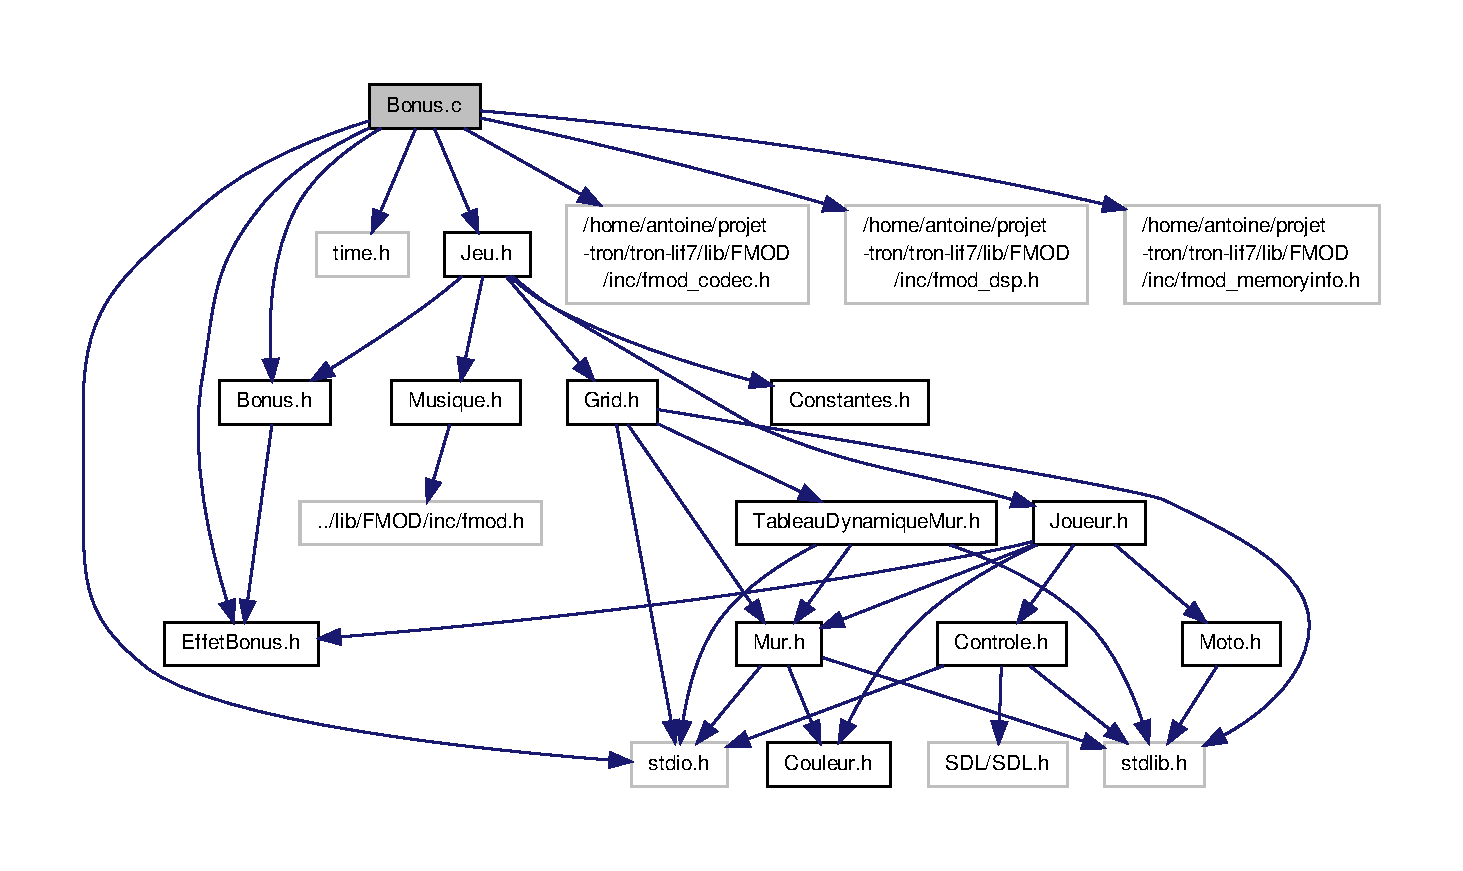
\includegraphics[width=350pt]{_bonus_8c__incl}
\end{center}
\end{figure}
\subsection*{Fonctions}
\begin{DoxyCompactItemize}
\item 
float \hyperlink{_bonus_8c_ad2300fc873c5fbb081462836491cf0af}{Bonus\-Get\-Position\-X} (const \hyperlink{struct_bonus}{Bonus} $\ast$bonus)
\item 
float \hyperlink{_bonus_8c_a96c6e41f28e13bebf9ec054be2adf162}{Bonus\-Get\-Position\-Y} (const \hyperlink{struct_bonus}{Bonus} $\ast$bonus)
\item 
unsigned int \hyperlink{_bonus_8c_a945a94dccbb8c3d86e7cfdd1d857b839}{Bonus\-Get\-Taille\-X} (const \hyperlink{struct_bonus}{Bonus} $\ast$bonus)
\item 
unsigned int \hyperlink{_bonus_8c_acb6e371434cd8f0a2344f82d9a6a1b3f}{Bonus\-Get\-Taille\-Y} (const \hyperlink{struct_bonus}{Bonus} $\ast$bonus)
\item 
\hyperlink{_effet_bonus_8h_a5c3ffd6a343fb8d5f63c87ee1a37a7fe}{Effet\-Bonus} \hyperlink{_bonus_8c_abe0dd0bc842a718d996ba2896c8b9095}{Bonus\-Get\-Effet\-Bonus} (const \hyperlink{struct_bonus}{Bonus} $\ast$bonus)
\item 
void \hyperlink{_bonus_8c_a3d2d99a0657d70c3f5377a6ff8086aa4}{Bonus\-Set\-Position\-X} (\hyperlink{struct_bonus}{Bonus} $\ast$bonus, float position\-X)
\item 
void \hyperlink{_bonus_8c_aee7509485ef9e5665df4f6ceb4c3e013}{Bonus\-Set\-Position\-Y} (\hyperlink{struct_bonus}{Bonus} $\ast$bonus, float position\-Y)
\item 
void \hyperlink{_bonus_8c_afcfcf285fd9d03b022fe35d7b7133617}{Bonus\-Set\-Taille\-X} (\hyperlink{struct_bonus}{Bonus} $\ast$bonus, unsigned int taille\-X)
\item 
void \hyperlink{_bonus_8c_a7dc1b0b791bc9511f058196149403618}{Bonus\-Set\-Taille\-Y} (\hyperlink{struct_bonus}{Bonus} $\ast$bonus, unsigned int taille\-Y)
\item 
void \hyperlink{_bonus_8c_a7ea8105e2bb249bf553667f8fa625938}{Bonus\-Set\-Effet\-Bonus} (\hyperlink{struct_bonus}{Bonus} $\ast$bonus, \hyperlink{_effet_bonus_8h_a5c3ffd6a343fb8d5f63c87ee1a37a7fe}{Effet\-Bonus} effet)
\item 
void \hyperlink{_bonus_8c_a50ea247d2b50e6bb7045adc1511b25f8}{Bonus\-Constructeur} (\hyperlink{struct_bonus}{Bonus} $\ast$bonus, float position\-X, float position\-Y, unsigned int taille\-X, unsigned int taille\-Y, \hyperlink{_effet_bonus_8h_a5c3ffd6a343fb8d5f63c87ee1a37a7fe}{Effet\-Bonus} effet)
\item 
void \hyperlink{_bonus_8c_a10400d2cfc7f4779aceaa86d8d65bfe1}{Bonus\-Destructeur} (\hyperlink{struct_bonus}{Bonus} $\ast$bonus)
\item 
void \hyperlink{_bonus_8c_add62f0ba957817fd53131c8b507fda71}{Bonus\-Test\-Regression} ()
\end{DoxyCompactItemize}


\subsection{Description détaillée}
\mbox{]} Module des \hyperlink{struct_bonus}{Bonus} du jeu \begin{DoxyAuthor}{Auteur}
\{Antoine.\-C,Matthieu.\-B\} 
\end{DoxyAuthor}
\begin{DoxyVersion}{Version}
1.\-1 
\end{DoxyVersion}
\begin{DoxyDate}{Date}
10 avril 2013 
\end{DoxyDate}


Définition dans le fichier \hyperlink{_bonus_8c_source}{Bonus.\-c}.



\subsection{Documentation des fonctions}
\hypertarget{_bonus_8c_a50ea247d2b50e6bb7045adc1511b25f8}{\index{Bonus.\-c@{Bonus.\-c}!Bonus\-Constructeur@{Bonus\-Constructeur}}
\index{Bonus\-Constructeur@{Bonus\-Constructeur}!Bonus.c@{Bonus.\-c}}
\subsubsection[{Bonus\-Constructeur}]{\setlength{\rightskip}{0pt plus 5cm}void Bonus\-Constructeur (
\begin{DoxyParamCaption}
\item[{{\bf Bonus} $\ast$}]{bonus, }
\item[{float}]{position\-X, }
\item[{float}]{position\-Y, }
\item[{unsigned int}]{taille\-X, }
\item[{unsigned int}]{taille\-Y, }
\item[{{\bf Effet\-Bonus}}]{effet}
\end{DoxyParamCaption}
)}}\label{_bonus_8c_a50ea247d2b50e6bb7045adc1511b25f8}


Définition à la ligne 48 du fichier Bonus.\-c.

\hypertarget{_bonus_8c_a10400d2cfc7f4779aceaa86d8d65bfe1}{\index{Bonus.\-c@{Bonus.\-c}!Bonus\-Destructeur@{Bonus\-Destructeur}}
\index{Bonus\-Destructeur@{Bonus\-Destructeur}!Bonus.c@{Bonus.\-c}}
\subsubsection[{Bonus\-Destructeur}]{\setlength{\rightskip}{0pt plus 5cm}void Bonus\-Destructeur (
\begin{DoxyParamCaption}
\item[{{\bf Bonus} $\ast$}]{bonus}
\end{DoxyParamCaption}
)}}\label{_bonus_8c_a10400d2cfc7f4779aceaa86d8d65bfe1}


Définition à la ligne 56 du fichier Bonus.\-c.

\hypertarget{_bonus_8c_abe0dd0bc842a718d996ba2896c8b9095}{\index{Bonus.\-c@{Bonus.\-c}!Bonus\-Get\-Effet\-Bonus@{Bonus\-Get\-Effet\-Bonus}}
\index{Bonus\-Get\-Effet\-Bonus@{Bonus\-Get\-Effet\-Bonus}!Bonus.c@{Bonus.\-c}}
\subsubsection[{Bonus\-Get\-Effet\-Bonus}]{\setlength{\rightskip}{0pt plus 5cm}{\bf Effet\-Bonus} Bonus\-Get\-Effet\-Bonus (
\begin{DoxyParamCaption}
\item[{const {\bf Bonus} $\ast$}]{bonus}
\end{DoxyParamCaption}
)}}\label{_bonus_8c_abe0dd0bc842a718d996ba2896c8b9095}


Définition à la ligne 27 du fichier Bonus.\-c.

\hypertarget{_bonus_8c_ad2300fc873c5fbb081462836491cf0af}{\index{Bonus.\-c@{Bonus.\-c}!Bonus\-Get\-Position\-X@{Bonus\-Get\-Position\-X}}
\index{Bonus\-Get\-Position\-X@{Bonus\-Get\-Position\-X}!Bonus.c@{Bonus.\-c}}
\subsubsection[{Bonus\-Get\-Position\-X}]{\setlength{\rightskip}{0pt plus 5cm}float Bonus\-Get\-Position\-X (
\begin{DoxyParamCaption}
\item[{const {\bf Bonus} $\ast$}]{bonus}
\end{DoxyParamCaption}
)}}\label{_bonus_8c_ad2300fc873c5fbb081462836491cf0af}


Définition à la ligne 15 du fichier Bonus.\-c.

\hypertarget{_bonus_8c_a96c6e41f28e13bebf9ec054be2adf162}{\index{Bonus.\-c@{Bonus.\-c}!Bonus\-Get\-Position\-Y@{Bonus\-Get\-Position\-Y}}
\index{Bonus\-Get\-Position\-Y@{Bonus\-Get\-Position\-Y}!Bonus.c@{Bonus.\-c}}
\subsubsection[{Bonus\-Get\-Position\-Y}]{\setlength{\rightskip}{0pt plus 5cm}float Bonus\-Get\-Position\-Y (
\begin{DoxyParamCaption}
\item[{const {\bf Bonus} $\ast$}]{bonus}
\end{DoxyParamCaption}
)}}\label{_bonus_8c_a96c6e41f28e13bebf9ec054be2adf162}


Définition à la ligne 18 du fichier Bonus.\-c.

\hypertarget{_bonus_8c_a945a94dccbb8c3d86e7cfdd1d857b839}{\index{Bonus.\-c@{Bonus.\-c}!Bonus\-Get\-Taille\-X@{Bonus\-Get\-Taille\-X}}
\index{Bonus\-Get\-Taille\-X@{Bonus\-Get\-Taille\-X}!Bonus.c@{Bonus.\-c}}
\subsubsection[{Bonus\-Get\-Taille\-X}]{\setlength{\rightskip}{0pt plus 5cm}unsigned int Bonus\-Get\-Taille\-X (
\begin{DoxyParamCaption}
\item[{const {\bf Bonus} $\ast$}]{bonus}
\end{DoxyParamCaption}
)}}\label{_bonus_8c_a945a94dccbb8c3d86e7cfdd1d857b839}


Définition à la ligne 21 du fichier Bonus.\-c.

\hypertarget{_bonus_8c_acb6e371434cd8f0a2344f82d9a6a1b3f}{\index{Bonus.\-c@{Bonus.\-c}!Bonus\-Get\-Taille\-Y@{Bonus\-Get\-Taille\-Y}}
\index{Bonus\-Get\-Taille\-Y@{Bonus\-Get\-Taille\-Y}!Bonus.c@{Bonus.\-c}}
\subsubsection[{Bonus\-Get\-Taille\-Y}]{\setlength{\rightskip}{0pt plus 5cm}unsigned int Bonus\-Get\-Taille\-Y (
\begin{DoxyParamCaption}
\item[{const {\bf Bonus} $\ast$}]{bonus}
\end{DoxyParamCaption}
)}}\label{_bonus_8c_acb6e371434cd8f0a2344f82d9a6a1b3f}


Définition à la ligne 24 du fichier Bonus.\-c.

\hypertarget{_bonus_8c_a7ea8105e2bb249bf553667f8fa625938}{\index{Bonus.\-c@{Bonus.\-c}!Bonus\-Set\-Effet\-Bonus@{Bonus\-Set\-Effet\-Bonus}}
\index{Bonus\-Set\-Effet\-Bonus@{Bonus\-Set\-Effet\-Bonus}!Bonus.c@{Bonus.\-c}}
\subsubsection[{Bonus\-Set\-Effet\-Bonus}]{\setlength{\rightskip}{0pt plus 5cm}void Bonus\-Set\-Effet\-Bonus (
\begin{DoxyParamCaption}
\item[{{\bf Bonus} $\ast$}]{bonus, }
\item[{{\bf Effet\-Bonus}}]{effet}
\end{DoxyParamCaption}
)}}\label{_bonus_8c_a7ea8105e2bb249bf553667f8fa625938}


Définition à la ligne 44 du fichier Bonus.\-c.

\hypertarget{_bonus_8c_a3d2d99a0657d70c3f5377a6ff8086aa4}{\index{Bonus.\-c@{Bonus.\-c}!Bonus\-Set\-Position\-X@{Bonus\-Set\-Position\-X}}
\index{Bonus\-Set\-Position\-X@{Bonus\-Set\-Position\-X}!Bonus.c@{Bonus.\-c}}
\subsubsection[{Bonus\-Set\-Position\-X}]{\setlength{\rightskip}{0pt plus 5cm}void Bonus\-Set\-Position\-X (
\begin{DoxyParamCaption}
\item[{{\bf Bonus} $\ast$}]{bonus, }
\item[{float}]{position\-X}
\end{DoxyParamCaption}
)}}\label{_bonus_8c_a3d2d99a0657d70c3f5377a6ff8086aa4}


Définition à la ligne 32 du fichier Bonus.\-c.

\hypertarget{_bonus_8c_aee7509485ef9e5665df4f6ceb4c3e013}{\index{Bonus.\-c@{Bonus.\-c}!Bonus\-Set\-Position\-Y@{Bonus\-Set\-Position\-Y}}
\index{Bonus\-Set\-Position\-Y@{Bonus\-Set\-Position\-Y}!Bonus.c@{Bonus.\-c}}
\subsubsection[{Bonus\-Set\-Position\-Y}]{\setlength{\rightskip}{0pt plus 5cm}void Bonus\-Set\-Position\-Y (
\begin{DoxyParamCaption}
\item[{{\bf Bonus} $\ast$}]{bonus, }
\item[{float}]{position\-Y}
\end{DoxyParamCaption}
)}}\label{_bonus_8c_aee7509485ef9e5665df4f6ceb4c3e013}


Définition à la ligne 35 du fichier Bonus.\-c.

\hypertarget{_bonus_8c_afcfcf285fd9d03b022fe35d7b7133617}{\index{Bonus.\-c@{Bonus.\-c}!Bonus\-Set\-Taille\-X@{Bonus\-Set\-Taille\-X}}
\index{Bonus\-Set\-Taille\-X@{Bonus\-Set\-Taille\-X}!Bonus.c@{Bonus.\-c}}
\subsubsection[{Bonus\-Set\-Taille\-X}]{\setlength{\rightskip}{0pt plus 5cm}void Bonus\-Set\-Taille\-X (
\begin{DoxyParamCaption}
\item[{{\bf Bonus} $\ast$}]{bonus, }
\item[{unsigned int}]{taille\-X}
\end{DoxyParamCaption}
)}}\label{_bonus_8c_afcfcf285fd9d03b022fe35d7b7133617}


Définition à la ligne 38 du fichier Bonus.\-c.

\hypertarget{_bonus_8c_a7dc1b0b791bc9511f058196149403618}{\index{Bonus.\-c@{Bonus.\-c}!Bonus\-Set\-Taille\-Y@{Bonus\-Set\-Taille\-Y}}
\index{Bonus\-Set\-Taille\-Y@{Bonus\-Set\-Taille\-Y}!Bonus.c@{Bonus.\-c}}
\subsubsection[{Bonus\-Set\-Taille\-Y}]{\setlength{\rightskip}{0pt plus 5cm}void Bonus\-Set\-Taille\-Y (
\begin{DoxyParamCaption}
\item[{{\bf Bonus} $\ast$}]{bonus, }
\item[{unsigned int}]{taille\-Y}
\end{DoxyParamCaption}
)}}\label{_bonus_8c_a7dc1b0b791bc9511f058196149403618}


Définition à la ligne 41 du fichier Bonus.\-c.

\hypertarget{_bonus_8c_add62f0ba957817fd53131c8b507fda71}{\index{Bonus.\-c@{Bonus.\-c}!Bonus\-Test\-Regression@{Bonus\-Test\-Regression}}
\index{Bonus\-Test\-Regression@{Bonus\-Test\-Regression}!Bonus.c@{Bonus.\-c}}
\subsubsection[{Bonus\-Test\-Regression}]{\setlength{\rightskip}{0pt plus 5cm}Bonus\-Test\-Regression (
\begin{DoxyParamCaption}
{}
\end{DoxyParamCaption}
)}}\label{_bonus_8c_add62f0ba957817fd53131c8b507fda71}
Test du Module 

Définition à la ligne 67 du fichier Bonus.\-c.


\hypertarget{_bonus_8h}{\section{Référence du fichier Bonus.\-h}
\label{_bonus_8h}\index{Bonus.\-h@{Bonus.\-h}}
}
{\ttfamily \#include \char`\"{}Effet\-Bonus.\-h\char`\"{}}\\*
Graphe des dépendances par inclusion de Bonus.\-h\-:\nopagebreak
\begin{figure}[H]
\begin{center}
\leavevmode
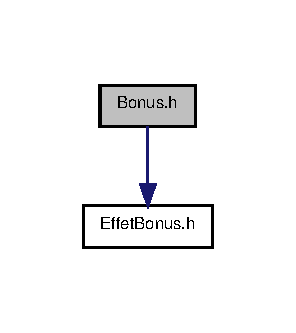
\includegraphics[width=154pt]{_bonus_8h__incl}
\end{center}
\end{figure}
Ce graphe montre quels fichiers incluent directement ou indirectement ce fichier \-:\nopagebreak
\begin{figure}[H]
\begin{center}
\leavevmode
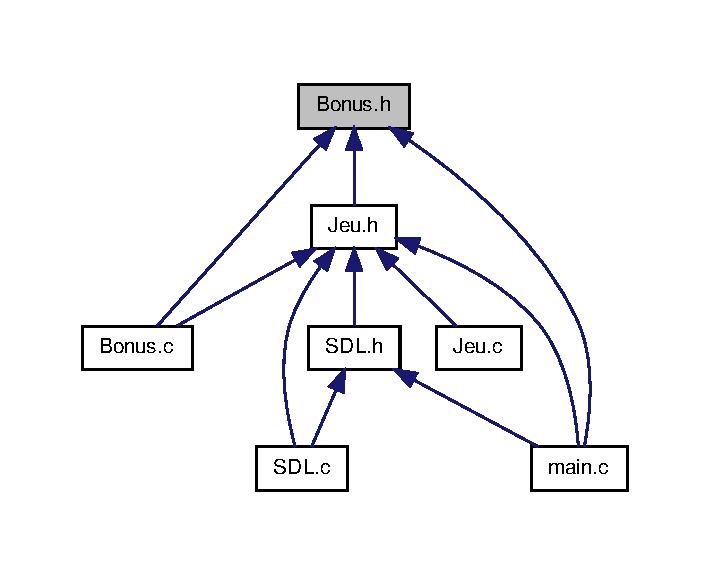
\includegraphics[width=341pt]{_bonus_8h__dep__incl}
\end{center}
\end{figure}
\subsection*{Structures de données}
\begin{DoxyCompactItemize}
\item 
struct \hyperlink{struct_bonus}{Bonus}
\end{DoxyCompactItemize}
\subsection*{Fonctions}
\begin{DoxyCompactItemize}
\item 
float \hyperlink{_bonus_8h_ad2300fc873c5fbb081462836491cf0af}{Bonus\-Get\-Position\-X} (const \hyperlink{struct_bonus}{Bonus} $\ast$bonus)
\item 
float \hyperlink{_bonus_8h_a96c6e41f28e13bebf9ec054be2adf162}{Bonus\-Get\-Position\-Y} (const \hyperlink{struct_bonus}{Bonus} $\ast$bonus)
\item 
unsigned int \hyperlink{_bonus_8h_a945a94dccbb8c3d86e7cfdd1d857b839}{Bonus\-Get\-Taille\-X} (const \hyperlink{struct_bonus}{Bonus} $\ast$bonus)
\item 
unsigned int \hyperlink{_bonus_8h_acb6e371434cd8f0a2344f82d9a6a1b3f}{Bonus\-Get\-Taille\-Y} (const \hyperlink{struct_bonus}{Bonus} $\ast$bonus)
\item 
\hyperlink{_effet_bonus_8h_a5c3ffd6a343fb8d5f63c87ee1a37a7fe}{Effet\-Bonus} \hyperlink{_bonus_8h_afed5301f763aaa743ed5b566127ac2ed}{Bonus\-Get\-Effet\-Bonus} (const \hyperlink{struct_bonus}{Bonus} $\ast$effet)
\item 
void \hyperlink{_bonus_8h_a3d2d99a0657d70c3f5377a6ff8086aa4}{Bonus\-Set\-Position\-X} (\hyperlink{struct_bonus}{Bonus} $\ast$bonus, float position\-X)
\item 
void \hyperlink{_bonus_8h_aee7509485ef9e5665df4f6ceb4c3e013}{Bonus\-Set\-Position\-Y} (\hyperlink{struct_bonus}{Bonus} $\ast$bonus, float position\-Y)
\item 
void \hyperlink{_bonus_8h_afcfcf285fd9d03b022fe35d7b7133617}{Bonus\-Set\-Taille\-X} (\hyperlink{struct_bonus}{Bonus} $\ast$bonus, unsigned int taille\-X)
\item 
void \hyperlink{_bonus_8h_a7dc1b0b791bc9511f058196149403618}{Bonus\-Set\-Taille\-Y} (\hyperlink{struct_bonus}{Bonus} $\ast$bonus, unsigned int taille\-Y)
\item 
void \hyperlink{_bonus_8h_a7ea8105e2bb249bf553667f8fa625938}{Bonus\-Set\-Effet\-Bonus} (\hyperlink{struct_bonus}{Bonus} $\ast$bonus, \hyperlink{_effet_bonus_8h_a5c3ffd6a343fb8d5f63c87ee1a37a7fe}{Effet\-Bonus} effet)
\item 
void \hyperlink{_bonus_8h_a50ea247d2b50e6bb7045adc1511b25f8}{Bonus\-Constructeur} (\hyperlink{struct_bonus}{Bonus} $\ast$bonus, float position\-X, float position\-Y, unsigned int taille\-X, unsigned int taille\-Y, \hyperlink{_effet_bonus_8h_a5c3ffd6a343fb8d5f63c87ee1a37a7fe}{Effet\-Bonus} effet)
\item 
void \hyperlink{_bonus_8h_a10400d2cfc7f4779aceaa86d8d65bfe1}{Bonus\-Destructeur} (\hyperlink{struct_bonus}{Bonus} $\ast$bonus)
\item 
void \hyperlink{_bonus_8h_aeb85fd9743a06ab60c5e6facdcde6980}{Bonus\-Test\-Regression} ()
\end{DoxyCompactItemize}


\subsection{Description détaillée}
\mbox{]} Module des \hyperlink{struct_bonus}{Bonus} du jeu \begin{DoxyAuthor}{Auteur}
\{Antoine.\-C,Matthieu.\-B\} 
\end{DoxyAuthor}
\begin{DoxyVersion}{Version}
1.\-1 
\end{DoxyVersion}
\begin{DoxyDate}{Date}
10 avril 2013 
\end{DoxyDate}


Définition dans le fichier \hyperlink{_bonus_8h_source}{Bonus.\-h}.



\subsection{Documentation des fonctions}
\hypertarget{_bonus_8h_a50ea247d2b50e6bb7045adc1511b25f8}{\index{Bonus.\-h@{Bonus.\-h}!Bonus\-Constructeur@{Bonus\-Constructeur}}
\index{Bonus\-Constructeur@{Bonus\-Constructeur}!Bonus.h@{Bonus.\-h}}
\subsubsection[{Bonus\-Constructeur}]{\setlength{\rightskip}{0pt plus 5cm}void Bonus\-Constructeur (
\begin{DoxyParamCaption}
\item[{{\bf Bonus} $\ast$}]{bonus, }
\item[{float}]{position\-X, }
\item[{float}]{position\-Y, }
\item[{unsigned int}]{taille\-X, }
\item[{unsigned int}]{taille\-Y, }
\item[{{\bf Effet\-Bonus}}]{effet}
\end{DoxyParamCaption}
)}}\label{_bonus_8h_a50ea247d2b50e6bb7045adc1511b25f8}


Définition à la ligne 48 du fichier Bonus.\-c.

\hypertarget{_bonus_8h_a10400d2cfc7f4779aceaa86d8d65bfe1}{\index{Bonus.\-h@{Bonus.\-h}!Bonus\-Destructeur@{Bonus\-Destructeur}}
\index{Bonus\-Destructeur@{Bonus\-Destructeur}!Bonus.h@{Bonus.\-h}}
\subsubsection[{Bonus\-Destructeur}]{\setlength{\rightskip}{0pt plus 5cm}void Bonus\-Destructeur (
\begin{DoxyParamCaption}
\item[{{\bf Bonus} $\ast$}]{bonus}
\end{DoxyParamCaption}
)}}\label{_bonus_8h_a10400d2cfc7f4779aceaa86d8d65bfe1}


Définition à la ligne 56 du fichier Bonus.\-c.

\hypertarget{_bonus_8h_afed5301f763aaa743ed5b566127ac2ed}{\index{Bonus.\-h@{Bonus.\-h}!Bonus\-Get\-Effet\-Bonus@{Bonus\-Get\-Effet\-Bonus}}
\index{Bonus\-Get\-Effet\-Bonus@{Bonus\-Get\-Effet\-Bonus}!Bonus.h@{Bonus.\-h}}
\subsubsection[{Bonus\-Get\-Effet\-Bonus}]{\setlength{\rightskip}{0pt plus 5cm}{\bf Effet\-Bonus} Bonus\-Get\-Effet\-Bonus (
\begin{DoxyParamCaption}
\item[{const {\bf Bonus} $\ast$}]{effet}
\end{DoxyParamCaption}
)}}\label{_bonus_8h_afed5301f763aaa743ed5b566127ac2ed}


Définition à la ligne 27 du fichier Bonus.\-c.

\hypertarget{_bonus_8h_ad2300fc873c5fbb081462836491cf0af}{\index{Bonus.\-h@{Bonus.\-h}!Bonus\-Get\-Position\-X@{Bonus\-Get\-Position\-X}}
\index{Bonus\-Get\-Position\-X@{Bonus\-Get\-Position\-X}!Bonus.h@{Bonus.\-h}}
\subsubsection[{Bonus\-Get\-Position\-X}]{\setlength{\rightskip}{0pt plus 5cm}float Bonus\-Get\-Position\-X (
\begin{DoxyParamCaption}
\item[{const {\bf Bonus} $\ast$}]{bonus}
\end{DoxyParamCaption}
)}}\label{_bonus_8h_ad2300fc873c5fbb081462836491cf0af}


Définition à la ligne 15 du fichier Bonus.\-c.

\hypertarget{_bonus_8h_a96c6e41f28e13bebf9ec054be2adf162}{\index{Bonus.\-h@{Bonus.\-h}!Bonus\-Get\-Position\-Y@{Bonus\-Get\-Position\-Y}}
\index{Bonus\-Get\-Position\-Y@{Bonus\-Get\-Position\-Y}!Bonus.h@{Bonus.\-h}}
\subsubsection[{Bonus\-Get\-Position\-Y}]{\setlength{\rightskip}{0pt plus 5cm}float Bonus\-Get\-Position\-Y (
\begin{DoxyParamCaption}
\item[{const {\bf Bonus} $\ast$}]{bonus}
\end{DoxyParamCaption}
)}}\label{_bonus_8h_a96c6e41f28e13bebf9ec054be2adf162}


Définition à la ligne 18 du fichier Bonus.\-c.

\hypertarget{_bonus_8h_a945a94dccbb8c3d86e7cfdd1d857b839}{\index{Bonus.\-h@{Bonus.\-h}!Bonus\-Get\-Taille\-X@{Bonus\-Get\-Taille\-X}}
\index{Bonus\-Get\-Taille\-X@{Bonus\-Get\-Taille\-X}!Bonus.h@{Bonus.\-h}}
\subsubsection[{Bonus\-Get\-Taille\-X}]{\setlength{\rightskip}{0pt plus 5cm}unsigned int Bonus\-Get\-Taille\-X (
\begin{DoxyParamCaption}
\item[{const {\bf Bonus} $\ast$}]{bonus}
\end{DoxyParamCaption}
)}}\label{_bonus_8h_a945a94dccbb8c3d86e7cfdd1d857b839}


Définition à la ligne 21 du fichier Bonus.\-c.

\hypertarget{_bonus_8h_acb6e371434cd8f0a2344f82d9a6a1b3f}{\index{Bonus.\-h@{Bonus.\-h}!Bonus\-Get\-Taille\-Y@{Bonus\-Get\-Taille\-Y}}
\index{Bonus\-Get\-Taille\-Y@{Bonus\-Get\-Taille\-Y}!Bonus.h@{Bonus.\-h}}
\subsubsection[{Bonus\-Get\-Taille\-Y}]{\setlength{\rightskip}{0pt plus 5cm}unsigned int Bonus\-Get\-Taille\-Y (
\begin{DoxyParamCaption}
\item[{const {\bf Bonus} $\ast$}]{bonus}
\end{DoxyParamCaption}
)}}\label{_bonus_8h_acb6e371434cd8f0a2344f82d9a6a1b3f}


Définition à la ligne 24 du fichier Bonus.\-c.

\hypertarget{_bonus_8h_a7ea8105e2bb249bf553667f8fa625938}{\index{Bonus.\-h@{Bonus.\-h}!Bonus\-Set\-Effet\-Bonus@{Bonus\-Set\-Effet\-Bonus}}
\index{Bonus\-Set\-Effet\-Bonus@{Bonus\-Set\-Effet\-Bonus}!Bonus.h@{Bonus.\-h}}
\subsubsection[{Bonus\-Set\-Effet\-Bonus}]{\setlength{\rightskip}{0pt plus 5cm}void Bonus\-Set\-Effet\-Bonus (
\begin{DoxyParamCaption}
\item[{{\bf Bonus} $\ast$}]{bonus, }
\item[{{\bf Effet\-Bonus}}]{effet}
\end{DoxyParamCaption}
)}}\label{_bonus_8h_a7ea8105e2bb249bf553667f8fa625938}


Définition à la ligne 44 du fichier Bonus.\-c.

\hypertarget{_bonus_8h_a3d2d99a0657d70c3f5377a6ff8086aa4}{\index{Bonus.\-h@{Bonus.\-h}!Bonus\-Set\-Position\-X@{Bonus\-Set\-Position\-X}}
\index{Bonus\-Set\-Position\-X@{Bonus\-Set\-Position\-X}!Bonus.h@{Bonus.\-h}}
\subsubsection[{Bonus\-Set\-Position\-X}]{\setlength{\rightskip}{0pt plus 5cm}void Bonus\-Set\-Position\-X (
\begin{DoxyParamCaption}
\item[{{\bf Bonus} $\ast$}]{bonus, }
\item[{float}]{position\-X}
\end{DoxyParamCaption}
)}}\label{_bonus_8h_a3d2d99a0657d70c3f5377a6ff8086aa4}


Définition à la ligne 32 du fichier Bonus.\-c.

\hypertarget{_bonus_8h_aee7509485ef9e5665df4f6ceb4c3e013}{\index{Bonus.\-h@{Bonus.\-h}!Bonus\-Set\-Position\-Y@{Bonus\-Set\-Position\-Y}}
\index{Bonus\-Set\-Position\-Y@{Bonus\-Set\-Position\-Y}!Bonus.h@{Bonus.\-h}}
\subsubsection[{Bonus\-Set\-Position\-Y}]{\setlength{\rightskip}{0pt plus 5cm}void Bonus\-Set\-Position\-Y (
\begin{DoxyParamCaption}
\item[{{\bf Bonus} $\ast$}]{bonus, }
\item[{float}]{position\-Y}
\end{DoxyParamCaption}
)}}\label{_bonus_8h_aee7509485ef9e5665df4f6ceb4c3e013}


Définition à la ligne 35 du fichier Bonus.\-c.

\hypertarget{_bonus_8h_afcfcf285fd9d03b022fe35d7b7133617}{\index{Bonus.\-h@{Bonus.\-h}!Bonus\-Set\-Taille\-X@{Bonus\-Set\-Taille\-X}}
\index{Bonus\-Set\-Taille\-X@{Bonus\-Set\-Taille\-X}!Bonus.h@{Bonus.\-h}}
\subsubsection[{Bonus\-Set\-Taille\-X}]{\setlength{\rightskip}{0pt plus 5cm}void Bonus\-Set\-Taille\-X (
\begin{DoxyParamCaption}
\item[{{\bf Bonus} $\ast$}]{bonus, }
\item[{unsigned int}]{taille\-X}
\end{DoxyParamCaption}
)}}\label{_bonus_8h_afcfcf285fd9d03b022fe35d7b7133617}


Définition à la ligne 38 du fichier Bonus.\-c.

\hypertarget{_bonus_8h_a7dc1b0b791bc9511f058196149403618}{\index{Bonus.\-h@{Bonus.\-h}!Bonus\-Set\-Taille\-Y@{Bonus\-Set\-Taille\-Y}}
\index{Bonus\-Set\-Taille\-Y@{Bonus\-Set\-Taille\-Y}!Bonus.h@{Bonus.\-h}}
\subsubsection[{Bonus\-Set\-Taille\-Y}]{\setlength{\rightskip}{0pt plus 5cm}void Bonus\-Set\-Taille\-Y (
\begin{DoxyParamCaption}
\item[{{\bf Bonus} $\ast$}]{bonus, }
\item[{unsigned int}]{taille\-Y}
\end{DoxyParamCaption}
)}}\label{_bonus_8h_a7dc1b0b791bc9511f058196149403618}


Définition à la ligne 41 du fichier Bonus.\-c.

\hypertarget{_bonus_8h_aeb85fd9743a06ab60c5e6facdcde6980}{\index{Bonus.\-h@{Bonus.\-h}!Bonus\-Test\-Regression@{Bonus\-Test\-Regression}}
\index{Bonus\-Test\-Regression@{Bonus\-Test\-Regression}!Bonus.h@{Bonus.\-h}}
\subsubsection[{Bonus\-Test\-Regression}]{\setlength{\rightskip}{0pt plus 5cm}void Bonus\-Test\-Regression (
\begin{DoxyParamCaption}
{}
\end{DoxyParamCaption}
)}}\label{_bonus_8h_aeb85fd9743a06ab60c5e6facdcde6980}
Test du Module 

Définition à la ligne 67 du fichier Bonus.\-c.


\hypertarget{_constantes_8h}{\section{Référence du fichier Constantes.\-h}
\label{_constantes_8h}\index{Constantes.\-h@{Constantes.\-h}}
}
Ce graphe montre quels fichiers incluent directement ou indirectement ce fichier \-:\nopagebreak
\begin{figure}[H]
\begin{center}
\leavevmode
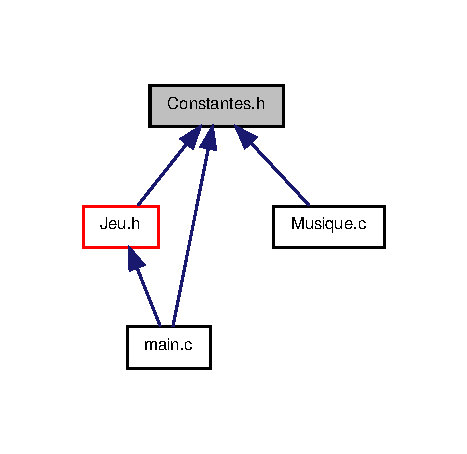
\includegraphics[width=224pt]{_constantes_8h__dep__incl}
\end{center}
\end{figure}
\subsection*{Macros}
\begin{DoxyCompactItemize}
\item 
\#define \hyperlink{_constantes_8h_a505b3b803482fbd73a5eafac78db730f}{\-\_\-\-Nombre\-\_\-de\-\_\-\-Joueur}~2
\item 
\#define \hyperlink{_constantes_8h_a5fb1c74112909224c5f7e80a8af4c2d0}{\-\_\-\-Nombre\-\_\-de\-\_\-\-Manette}~0
\item 
\#define \hyperlink{_constantes_8h_ad8b40dec44c44014644f995661e4d56a}{\-\_\-\-Nombre\-\_\-\-I\-A}~1
\item 
\#define \hyperlink{_constantes_8h_a1d2abfb089da90098808b80c3e928584}{\-\_\-\-Score\-\_\-de\-\_\-\-Victoire}~14
\item 
\#define \hyperlink{_constantes_8h_a64872e3ddf1efd6847f90dbcb0ed21ce}{\-\_\-\-Nombre\-\_\-de\-\_\-\-Textes}~4
\item 
\#define \hyperlink{_constantes_8h_a228aa6ff538af983b44e972225d962b9}{\-\_\-\-Nombre\-\_\-\-Images\-\_\-\-Interface}~2
\item 
\#define \hyperlink{_constantes_8h_ad60a84514a894329c7591d677398f170}{\-\_\-\-Position\-\_\-\-X\-\_\-\-Grille}~5
\item 
\#define \hyperlink{_constantes_8h_a7b73a5db39ad602a8846e9074cdef48f}{\-\_\-\-Position\-\_\-\-Y\-\_\-\-Grille}~5
\item 
\#define \hyperlink{_constantes_8h_a22ca4a20964744e6df65d2c81d5b41ff}{\-\_\-\-Taille\-\_\-\-X\-\_\-\-Grille}~1000
\item 
\#define \hyperlink{_constantes_8h_abf68bdf8402080e47166e730e6fa7839}{\-\_\-\-Taille\-\_\-\-Y\-\_\-\-Grille}~700
\item 
\#define \hyperlink{_constantes_8h_a5486e43da0e415d8e657b6404134e6b7}{\-\_\-\-Precision\-\_\-\-Analyse\-\_\-\-I\-A}~10
\item 
\#define \hyperlink{_constantes_8h_abc403e70c3c3dfbdcb3c800cb192571b}{\-\_\-\-Duree\-\_\-\-Vie\-\_\-\-Mur}~150
\item 
\#define \hyperlink{_constantes_8h_a612d10894e13a2f3a1784441ed77abd0}{\-\_\-\-Vitesse\-\_\-\-Initiale}~10
\item 
\#define \hyperlink{_constantes_8h_a54979d8e6180f1971c1fb3d5a885451c}{\-\_\-\-Acceleration}~0.\-02f
\item 
\#define \hyperlink{_constantes_8h_af4e31715ab308023d6200e64b86b9946}{\-\_\-\-Nombre\-\_\-de\-\_\-\-Bonus}~4
\item 
\#define \hyperlink{_constantes_8h_aa8107d46dd4716d82da9d2a2c236784b}{\-\_\-\-Temps\-\_\-\-Bonus\-\_\-\-Boost}~25
\item 
\#define \hyperlink{_constantes_8h_a296e74aa0c165600fc9911ac06edd2bc}{\-\_\-\-Temps\-\_\-\-Bonus\-\_\-\-Saut}~5
\item 
\#define \hyperlink{_constantes_8h_a8e9754a93f3dc0c1263aa8ee9bdcda97}{\-\_\-\-Vitesse\-\_\-\-Boost}~15
\end{DoxyCompactItemize}


\subsection{Description détaillée}
\mbox{]} Module des constantes du jeu \begin{DoxyAuthor}{Auteur}
\{Antoine.\-C,Matthieu.\-B\} 
\end{DoxyAuthor}
\begin{DoxyVersion}{Version}
0.\-1 
\end{DoxyVersion}
\begin{DoxyDate}{Date}
2 avril 2013 
\end{DoxyDate}


Définition dans le fichier \hyperlink{_constantes_8h_source}{Constantes.\-h}.



\subsection{Documentation des macros}
\hypertarget{_constantes_8h_a54979d8e6180f1971c1fb3d5a885451c}{\index{Constantes.\-h@{Constantes.\-h}!\-\_\-\-Acceleration@{\-\_\-\-Acceleration}}
\index{\-\_\-\-Acceleration@{\-\_\-\-Acceleration}!Constantes.h@{Constantes.\-h}}
\subsubsection[{\-\_\-\-Acceleration}]{\setlength{\rightskip}{0pt plus 5cm}\#define \-\_\-\-Acceleration~0.\-02f}}\label{_constantes_8h_a54979d8e6180f1971c1fb3d5a885451c}


Définition à la ligne 29 du fichier Constantes.\-h.

\hypertarget{_constantes_8h_abc403e70c3c3dfbdcb3c800cb192571b}{\index{Constantes.\-h@{Constantes.\-h}!\-\_\-\-Duree\-\_\-\-Vie\-\_\-\-Mur@{\-\_\-\-Duree\-\_\-\-Vie\-\_\-\-Mur}}
\index{\-\_\-\-Duree\-\_\-\-Vie\-\_\-\-Mur@{\-\_\-\-Duree\-\_\-\-Vie\-\_\-\-Mur}!Constantes.h@{Constantes.\-h}}
\subsubsection[{\-\_\-\-Duree\-\_\-\-Vie\-\_\-\-Mur}]{\setlength{\rightskip}{0pt plus 5cm}\#define \-\_\-\-Duree\-\_\-\-Vie\-\_\-\-Mur~150}}\label{_constantes_8h_abc403e70c3c3dfbdcb3c800cb192571b}


Définition à la ligne 27 du fichier Constantes.\-h.

\hypertarget{_constantes_8h_af4e31715ab308023d6200e64b86b9946}{\index{Constantes.\-h@{Constantes.\-h}!\-\_\-\-Nombre\-\_\-de\-\_\-\-Bonus@{\-\_\-\-Nombre\-\_\-de\-\_\-\-Bonus}}
\index{\-\_\-\-Nombre\-\_\-de\-\_\-\-Bonus@{\-\_\-\-Nombre\-\_\-de\-\_\-\-Bonus}!Constantes.h@{Constantes.\-h}}
\subsubsection[{\-\_\-\-Nombre\-\_\-de\-\_\-\-Bonus}]{\setlength{\rightskip}{0pt plus 5cm}\#define \-\_\-\-Nombre\-\_\-de\-\_\-\-Bonus~4}}\label{_constantes_8h_af4e31715ab308023d6200e64b86b9946}


Définition à la ligne 31 du fichier Constantes.\-h.

\hypertarget{_constantes_8h_a505b3b803482fbd73a5eafac78db730f}{\index{Constantes.\-h@{Constantes.\-h}!\-\_\-\-Nombre\-\_\-de\-\_\-\-Joueur@{\-\_\-\-Nombre\-\_\-de\-\_\-\-Joueur}}
\index{\-\_\-\-Nombre\-\_\-de\-\_\-\-Joueur@{\-\_\-\-Nombre\-\_\-de\-\_\-\-Joueur}!Constantes.h@{Constantes.\-h}}
\subsubsection[{\-\_\-\-Nombre\-\_\-de\-\_\-\-Joueur}]{\setlength{\rightskip}{0pt plus 5cm}\#define \-\_\-\-Nombre\-\_\-de\-\_\-\-Joueur~2}}\label{_constantes_8h_a505b3b803482fbd73a5eafac78db730f}


Définition à la ligne 11 du fichier Constantes.\-h.

\hypertarget{_constantes_8h_a5fb1c74112909224c5f7e80a8af4c2d0}{\index{Constantes.\-h@{Constantes.\-h}!\-\_\-\-Nombre\-\_\-de\-\_\-\-Manette@{\-\_\-\-Nombre\-\_\-de\-\_\-\-Manette}}
\index{\-\_\-\-Nombre\-\_\-de\-\_\-\-Manette@{\-\_\-\-Nombre\-\_\-de\-\_\-\-Manette}!Constantes.h@{Constantes.\-h}}
\subsubsection[{\-\_\-\-Nombre\-\_\-de\-\_\-\-Manette}]{\setlength{\rightskip}{0pt plus 5cm}\#define \-\_\-\-Nombre\-\_\-de\-\_\-\-Manette~0}}\label{_constantes_8h_a5fb1c74112909224c5f7e80a8af4c2d0}


Définition à la ligne 12 du fichier Constantes.\-h.

\hypertarget{_constantes_8h_a64872e3ddf1efd6847f90dbcb0ed21ce}{\index{Constantes.\-h@{Constantes.\-h}!\-\_\-\-Nombre\-\_\-de\-\_\-\-Textes@{\-\_\-\-Nombre\-\_\-de\-\_\-\-Textes}}
\index{\-\_\-\-Nombre\-\_\-de\-\_\-\-Textes@{\-\_\-\-Nombre\-\_\-de\-\_\-\-Textes}!Constantes.h@{Constantes.\-h}}
\subsubsection[{\-\_\-\-Nombre\-\_\-de\-\_\-\-Textes}]{\setlength{\rightskip}{0pt plus 5cm}\#define \-\_\-\-Nombre\-\_\-de\-\_\-\-Textes~4}}\label{_constantes_8h_a64872e3ddf1efd6847f90dbcb0ed21ce}


Définition à la ligne 17 du fichier Constantes.\-h.

\hypertarget{_constantes_8h_ad8b40dec44c44014644f995661e4d56a}{\index{Constantes.\-h@{Constantes.\-h}!\-\_\-\-Nombre\-\_\-\-I\-A@{\-\_\-\-Nombre\-\_\-\-I\-A}}
\index{\-\_\-\-Nombre\-\_\-\-I\-A@{\-\_\-\-Nombre\-\_\-\-I\-A}!Constantes.h@{Constantes.\-h}}
\subsubsection[{\-\_\-\-Nombre\-\_\-\-I\-A}]{\setlength{\rightskip}{0pt plus 5cm}\#define \-\_\-\-Nombre\-\_\-\-I\-A~1}}\label{_constantes_8h_ad8b40dec44c44014644f995661e4d56a}


Définition à la ligne 13 du fichier Constantes.\-h.

\hypertarget{_constantes_8h_a228aa6ff538af983b44e972225d962b9}{\index{Constantes.\-h@{Constantes.\-h}!\-\_\-\-Nombre\-\_\-\-Images\-\_\-\-Interface@{\-\_\-\-Nombre\-\_\-\-Images\-\_\-\-Interface}}
\index{\-\_\-\-Nombre\-\_\-\-Images\-\_\-\-Interface@{\-\_\-\-Nombre\-\_\-\-Images\-\_\-\-Interface}!Constantes.h@{Constantes.\-h}}
\subsubsection[{\-\_\-\-Nombre\-\_\-\-Images\-\_\-\-Interface}]{\setlength{\rightskip}{0pt plus 5cm}\#define \-\_\-\-Nombre\-\_\-\-Images\-\_\-\-Interface~2}}\label{_constantes_8h_a228aa6ff538af983b44e972225d962b9}


Définition à la ligne 18 du fichier Constantes.\-h.

\hypertarget{_constantes_8h_ad60a84514a894329c7591d677398f170}{\index{Constantes.\-h@{Constantes.\-h}!\-\_\-\-Position\-\_\-\-X\-\_\-\-Grille@{\-\_\-\-Position\-\_\-\-X\-\_\-\-Grille}}
\index{\-\_\-\-Position\-\_\-\-X\-\_\-\-Grille@{\-\_\-\-Position\-\_\-\-X\-\_\-\-Grille}!Constantes.h@{Constantes.\-h}}
\subsubsection[{\-\_\-\-Position\-\_\-\-X\-\_\-\-Grille}]{\setlength{\rightskip}{0pt plus 5cm}\#define \-\_\-\-Position\-\_\-\-X\-\_\-\-Grille~5}}\label{_constantes_8h_ad60a84514a894329c7591d677398f170}


Définition à la ligne 20 du fichier Constantes.\-h.

\hypertarget{_constantes_8h_a7b73a5db39ad602a8846e9074cdef48f}{\index{Constantes.\-h@{Constantes.\-h}!\-\_\-\-Position\-\_\-\-Y\-\_\-\-Grille@{\-\_\-\-Position\-\_\-\-Y\-\_\-\-Grille}}
\index{\-\_\-\-Position\-\_\-\-Y\-\_\-\-Grille@{\-\_\-\-Position\-\_\-\-Y\-\_\-\-Grille}!Constantes.h@{Constantes.\-h}}
\subsubsection[{\-\_\-\-Position\-\_\-\-Y\-\_\-\-Grille}]{\setlength{\rightskip}{0pt plus 5cm}\#define \-\_\-\-Position\-\_\-\-Y\-\_\-\-Grille~5}}\label{_constantes_8h_a7b73a5db39ad602a8846e9074cdef48f}


Définition à la ligne 21 du fichier Constantes.\-h.

\hypertarget{_constantes_8h_a5486e43da0e415d8e657b6404134e6b7}{\index{Constantes.\-h@{Constantes.\-h}!\-\_\-\-Precision\-\_\-\-Analyse\-\_\-\-I\-A@{\-\_\-\-Precision\-\_\-\-Analyse\-\_\-\-I\-A}}
\index{\-\_\-\-Precision\-\_\-\-Analyse\-\_\-\-I\-A@{\-\_\-\-Precision\-\_\-\-Analyse\-\_\-\-I\-A}!Constantes.h@{Constantes.\-h}}
\subsubsection[{\-\_\-\-Precision\-\_\-\-Analyse\-\_\-\-I\-A}]{\setlength{\rightskip}{0pt plus 5cm}\#define \-\_\-\-Precision\-\_\-\-Analyse\-\_\-\-I\-A~10}}\label{_constantes_8h_a5486e43da0e415d8e657b6404134e6b7}


Définition à la ligne 25 du fichier Constantes.\-h.

\hypertarget{_constantes_8h_a1d2abfb089da90098808b80c3e928584}{\index{Constantes.\-h@{Constantes.\-h}!\-\_\-\-Score\-\_\-de\-\_\-\-Victoire@{\-\_\-\-Score\-\_\-de\-\_\-\-Victoire}}
\index{\-\_\-\-Score\-\_\-de\-\_\-\-Victoire@{\-\_\-\-Score\-\_\-de\-\_\-\-Victoire}!Constantes.h@{Constantes.\-h}}
\subsubsection[{\-\_\-\-Score\-\_\-de\-\_\-\-Victoire}]{\setlength{\rightskip}{0pt plus 5cm}\#define \-\_\-\-Score\-\_\-de\-\_\-\-Victoire~14}}\label{_constantes_8h_a1d2abfb089da90098808b80c3e928584}


Définition à la ligne 15 du fichier Constantes.\-h.

\hypertarget{_constantes_8h_a22ca4a20964744e6df65d2c81d5b41ff}{\index{Constantes.\-h@{Constantes.\-h}!\-\_\-\-Taille\-\_\-\-X\-\_\-\-Grille@{\-\_\-\-Taille\-\_\-\-X\-\_\-\-Grille}}
\index{\-\_\-\-Taille\-\_\-\-X\-\_\-\-Grille@{\-\_\-\-Taille\-\_\-\-X\-\_\-\-Grille}!Constantes.h@{Constantes.\-h}}
\subsubsection[{\-\_\-\-Taille\-\_\-\-X\-\_\-\-Grille}]{\setlength{\rightskip}{0pt plus 5cm}\#define \-\_\-\-Taille\-\_\-\-X\-\_\-\-Grille~1000}}\label{_constantes_8h_a22ca4a20964744e6df65d2c81d5b41ff}


Définition à la ligne 22 du fichier Constantes.\-h.

\hypertarget{_constantes_8h_abf68bdf8402080e47166e730e6fa7839}{\index{Constantes.\-h@{Constantes.\-h}!\-\_\-\-Taille\-\_\-\-Y\-\_\-\-Grille@{\-\_\-\-Taille\-\_\-\-Y\-\_\-\-Grille}}
\index{\-\_\-\-Taille\-\_\-\-Y\-\_\-\-Grille@{\-\_\-\-Taille\-\_\-\-Y\-\_\-\-Grille}!Constantes.h@{Constantes.\-h}}
\subsubsection[{\-\_\-\-Taille\-\_\-\-Y\-\_\-\-Grille}]{\setlength{\rightskip}{0pt plus 5cm}\#define \-\_\-\-Taille\-\_\-\-Y\-\_\-\-Grille~700}}\label{_constantes_8h_abf68bdf8402080e47166e730e6fa7839}


Définition à la ligne 23 du fichier Constantes.\-h.

\hypertarget{_constantes_8h_aa8107d46dd4716d82da9d2a2c236784b}{\index{Constantes.\-h@{Constantes.\-h}!\-\_\-\-Temps\-\_\-\-Bonus\-\_\-\-Boost@{\-\_\-\-Temps\-\_\-\-Bonus\-\_\-\-Boost}}
\index{\-\_\-\-Temps\-\_\-\-Bonus\-\_\-\-Boost@{\-\_\-\-Temps\-\_\-\-Bonus\-\_\-\-Boost}!Constantes.h@{Constantes.\-h}}
\subsubsection[{\-\_\-\-Temps\-\_\-\-Bonus\-\_\-\-Boost}]{\setlength{\rightskip}{0pt plus 5cm}\#define \-\_\-\-Temps\-\_\-\-Bonus\-\_\-\-Boost~25}}\label{_constantes_8h_aa8107d46dd4716d82da9d2a2c236784b}


Définition à la ligne 32 du fichier Constantes.\-h.

\hypertarget{_constantes_8h_a296e74aa0c165600fc9911ac06edd2bc}{\index{Constantes.\-h@{Constantes.\-h}!\-\_\-\-Temps\-\_\-\-Bonus\-\_\-\-Saut@{\-\_\-\-Temps\-\_\-\-Bonus\-\_\-\-Saut}}
\index{\-\_\-\-Temps\-\_\-\-Bonus\-\_\-\-Saut@{\-\_\-\-Temps\-\_\-\-Bonus\-\_\-\-Saut}!Constantes.h@{Constantes.\-h}}
\subsubsection[{\-\_\-\-Temps\-\_\-\-Bonus\-\_\-\-Saut}]{\setlength{\rightskip}{0pt plus 5cm}\#define \-\_\-\-Temps\-\_\-\-Bonus\-\_\-\-Saut~5}}\label{_constantes_8h_a296e74aa0c165600fc9911ac06edd2bc}


Définition à la ligne 33 du fichier Constantes.\-h.

\hypertarget{_constantes_8h_a8e9754a93f3dc0c1263aa8ee9bdcda97}{\index{Constantes.\-h@{Constantes.\-h}!\-\_\-\-Vitesse\-\_\-\-Boost@{\-\_\-\-Vitesse\-\_\-\-Boost}}
\index{\-\_\-\-Vitesse\-\_\-\-Boost@{\-\_\-\-Vitesse\-\_\-\-Boost}!Constantes.h@{Constantes.\-h}}
\subsubsection[{\-\_\-\-Vitesse\-\_\-\-Boost}]{\setlength{\rightskip}{0pt plus 5cm}\#define \-\_\-\-Vitesse\-\_\-\-Boost~15}}\label{_constantes_8h_a8e9754a93f3dc0c1263aa8ee9bdcda97}


Définition à la ligne 34 du fichier Constantes.\-h.

\hypertarget{_constantes_8h_a612d10894e13a2f3a1784441ed77abd0}{\index{Constantes.\-h@{Constantes.\-h}!\-\_\-\-Vitesse\-\_\-\-Initiale@{\-\_\-\-Vitesse\-\_\-\-Initiale}}
\index{\-\_\-\-Vitesse\-\_\-\-Initiale@{\-\_\-\-Vitesse\-\_\-\-Initiale}!Constantes.h@{Constantes.\-h}}
\subsubsection[{\-\_\-\-Vitesse\-\_\-\-Initiale}]{\setlength{\rightskip}{0pt plus 5cm}\#define \-\_\-\-Vitesse\-\_\-\-Initiale~10}}\label{_constantes_8h_a612d10894e13a2f3a1784441ed77abd0}


Définition à la ligne 28 du fichier Constantes.\-h.


\hypertarget{_controle_8c}{\section{Référence du fichier Controle.\-c}
\label{_controle_8c}\index{Controle.\-c@{Controle.\-c}}
}
{\ttfamily \#include \char`\"{}Controle.\-h\char`\"{}}\\*
{\ttfamily \#include $<$stdlib.\-h$>$}\\*
{\ttfamily \#include $<$stdio.\-h$>$}\\*
{\ttfamily \#include $<$assert.\-h$>$}\\*
{\ttfamily \#include $<$S\-D\-L/\-S\-D\-L.\-h$>$}\\*
Graphe des dépendances par inclusion de Controle.\-c\-:\nopagebreak
\begin{figure}[H]
\begin{center}
\leavevmode
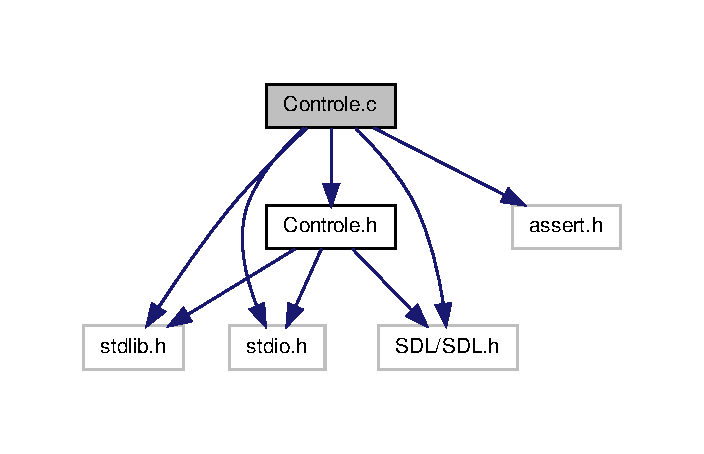
\includegraphics[width=317pt]{_controle_8c__incl}
\end{center}
\end{figure}
\subsection*{Fonctions}
\begin{DoxyCompactItemize}
\item 
S\-D\-L\-Key \hyperlink{_controle_8c_aceb59e2dc81ee481b6f4e4512451ca2c}{Controle\-Get\-Droite} (const \hyperlink{struct_controle}{Controle} $\ast$controle)
\item 
S\-D\-L\-Key \hyperlink{_controle_8c_a58b4a2d8f6f6248519b47d045d205144}{Controle\-Get\-Haut} (const \hyperlink{struct_controle}{Controle} $\ast$controle)
\item 
S\-D\-L\-Key \hyperlink{_controle_8c_a2e052af3b9995a418ffae3f816068c40}{Controle\-Get\-Gauche} (const \hyperlink{struct_controle}{Controle} $\ast$controle)
\item 
S\-D\-L\-Key \hyperlink{_controle_8c_afbc4a836ab3364317147c49c68071191}{Controle\-Get\-Bas} (const \hyperlink{struct_controle}{Controle} $\ast$controle)
\item 
S\-D\-L\-Key \hyperlink{_controle_8c_a777b3cf5baab32a2048abd6c334ee1cf}{Controle\-Get\-Bonus} (const \hyperlink{struct_controle}{Controle} $\ast$controle)
\item 
void \hyperlink{_controle_8c_ac551619cdc29f2173ec6a2b528793f20}{Controle\-Set\-Droite} (\hyperlink{struct_controle}{Controle} $\ast$controle, S\-D\-L\-Key x)
\item 
void \hyperlink{_controle_8c_afdede420fafbf282b46f799ae0bfcb4b}{Controle\-Set\-Haut} (\hyperlink{struct_controle}{Controle} $\ast$controle, S\-D\-L\-Key x)
\item 
void \hyperlink{_controle_8c_a8d64b2f88ae1accc2fb58a7a394fe904}{Controle\-Set\-Gauche} (\hyperlink{struct_controle}{Controle} $\ast$controle, S\-D\-L\-Key x)
\item 
void \hyperlink{_controle_8c_a9d8236e4578c1941fa13c7713bc1b9c2}{Controle\-Set\-Bas} (\hyperlink{struct_controle}{Controle} $\ast$controle, S\-D\-L\-Key x)
\item 
void \hyperlink{_controle_8c_a53dc76310eaee419e4d0d1b3d5e39003}{Controle\-Set\-Bonus} (\hyperlink{struct_controle}{Controle} $\ast$controle, S\-D\-L\-Key x)
\item 
void \hyperlink{_controle_8c_a3097aea62abd4e67f4c319756ad88a0e}{Controle\-Constructeur} (\hyperlink{struct_controle}{Controle} $\ast$controle, S\-D\-L\-Key haut, S\-D\-L\-Key bas, S\-D\-L\-Key gauche, S\-D\-L\-Key droite, S\-D\-L\-Key bonus)
\item 
void \hyperlink{_controle_8c_af1bb24fb9790dc018f7396c15e7b47a0}{Controle\-Destructeur} (\hyperlink{struct_controle}{Controle} $\ast$controle)
\item 
void \hyperlink{_controle_8c_a49d6667e80a116e40db1741c08616600}{Controle\-Test\-Regression} ()
\end{DoxyCompactItemize}


\subsection{Description détaillée}
\mbox{]} Module qui défini les Controles \begin{DoxyAuthor}{Auteur}
\{Antoine.\-C,Matthieu.\-B\} 
\end{DoxyAuthor}
\begin{DoxyVersion}{Version}
0.\-1 
\end{DoxyVersion}
\begin{DoxyDate}{Date}
13 mars 2013 
\end{DoxyDate}


Définition dans le fichier \hyperlink{_controle_8c_source}{Controle.\-c}.



\subsection{Documentation des fonctions}
\hypertarget{_controle_8c_a3097aea62abd4e67f4c319756ad88a0e}{\index{Controle.\-c@{Controle.\-c}!Controle\-Constructeur@{Controle\-Constructeur}}
\index{Controle\-Constructeur@{Controle\-Constructeur}!Controle.c@{Controle.\-c}}
\subsubsection[{Controle\-Constructeur}]{\setlength{\rightskip}{0pt plus 5cm}void Controle\-Constructeur (
\begin{DoxyParamCaption}
\item[{{\bf Controle} $\ast$}]{controle, }
\item[{S\-D\-L\-Key}]{haut, }
\item[{S\-D\-L\-Key}]{bas, }
\item[{S\-D\-L\-Key}]{gauche, }
\item[{S\-D\-L\-Key}]{droite, }
\item[{S\-D\-L\-Key}]{bonus}
\end{DoxyParamCaption}
)}}\label{_controle_8c_a3097aea62abd4e67f4c319756ad88a0e}


Définition à la ligne 49 du fichier Controle.\-c.

\hypertarget{_controle_8c_af1bb24fb9790dc018f7396c15e7b47a0}{\index{Controle.\-c@{Controle.\-c}!Controle\-Destructeur@{Controle\-Destructeur}}
\index{Controle\-Destructeur@{Controle\-Destructeur}!Controle.c@{Controle.\-c}}
\subsubsection[{Controle\-Destructeur}]{\setlength{\rightskip}{0pt plus 5cm}void Controle\-Destructeur (
\begin{DoxyParamCaption}
\item[{{\bf Controle} $\ast$}]{controle}
\end{DoxyParamCaption}
)}}\label{_controle_8c_af1bb24fb9790dc018f7396c15e7b47a0}


Définition à la ligne 57 du fichier Controle.\-c.

\hypertarget{_controle_8c_afbc4a836ab3364317147c49c68071191}{\index{Controle.\-c@{Controle.\-c}!Controle\-Get\-Bas@{Controle\-Get\-Bas}}
\index{Controle\-Get\-Bas@{Controle\-Get\-Bas}!Controle.c@{Controle.\-c}}
\subsubsection[{Controle\-Get\-Bas}]{\setlength{\rightskip}{0pt plus 5cm}S\-D\-L\-Key Controle\-Get\-Bas (
\begin{DoxyParamCaption}
\item[{const {\bf Controle} $\ast$}]{controle}
\end{DoxyParamCaption}
)}}\label{_controle_8c_afbc4a836ab3364317147c49c68071191}


Définition à la ligne 24 du fichier Controle.\-c.

\hypertarget{_controle_8c_a777b3cf5baab32a2048abd6c334ee1cf}{\index{Controle.\-c@{Controle.\-c}!Controle\-Get\-Bonus@{Controle\-Get\-Bonus}}
\index{Controle\-Get\-Bonus@{Controle\-Get\-Bonus}!Controle.c@{Controle.\-c}}
\subsubsection[{Controle\-Get\-Bonus}]{\setlength{\rightskip}{0pt plus 5cm}S\-D\-L\-Key Controle\-Get\-Bonus (
\begin{DoxyParamCaption}
\item[{const {\bf Controle} $\ast$}]{controle}
\end{DoxyParamCaption}
)}}\label{_controle_8c_a777b3cf5baab32a2048abd6c334ee1cf}


Définition à la ligne 28 du fichier Controle.\-c.

\hypertarget{_controle_8c_aceb59e2dc81ee481b6f4e4512451ca2c}{\index{Controle.\-c@{Controle.\-c}!Controle\-Get\-Droite@{Controle\-Get\-Droite}}
\index{Controle\-Get\-Droite@{Controle\-Get\-Droite}!Controle.c@{Controle.\-c}}
\subsubsection[{Controle\-Get\-Droite}]{\setlength{\rightskip}{0pt plus 5cm}S\-D\-L\-Key Controle\-Get\-Droite (
\begin{DoxyParamCaption}
\item[{const {\bf Controle} $\ast$}]{controle}
\end{DoxyParamCaption}
)}}\label{_controle_8c_aceb59e2dc81ee481b6f4e4512451ca2c}


Définition à la ligne 15 du fichier Controle.\-c.

\hypertarget{_controle_8c_a2e052af3b9995a418ffae3f816068c40}{\index{Controle.\-c@{Controle.\-c}!Controle\-Get\-Gauche@{Controle\-Get\-Gauche}}
\index{Controle\-Get\-Gauche@{Controle\-Get\-Gauche}!Controle.c@{Controle.\-c}}
\subsubsection[{Controle\-Get\-Gauche}]{\setlength{\rightskip}{0pt plus 5cm}S\-D\-L\-Key Controle\-Get\-Gauche (
\begin{DoxyParamCaption}
\item[{const {\bf Controle} $\ast$}]{controle}
\end{DoxyParamCaption}
)}}\label{_controle_8c_a2e052af3b9995a418ffae3f816068c40}


Définition à la ligne 21 du fichier Controle.\-c.

\hypertarget{_controle_8c_a58b4a2d8f6f6248519b47d045d205144}{\index{Controle.\-c@{Controle.\-c}!Controle\-Get\-Haut@{Controle\-Get\-Haut}}
\index{Controle\-Get\-Haut@{Controle\-Get\-Haut}!Controle.c@{Controle.\-c}}
\subsubsection[{Controle\-Get\-Haut}]{\setlength{\rightskip}{0pt plus 5cm}S\-D\-L\-Key Controle\-Get\-Haut (
\begin{DoxyParamCaption}
\item[{const {\bf Controle} $\ast$}]{controle}
\end{DoxyParamCaption}
)}}\label{_controle_8c_a58b4a2d8f6f6248519b47d045d205144}


Définition à la ligne 18 du fichier Controle.\-c.

\hypertarget{_controle_8c_a9d8236e4578c1941fa13c7713bc1b9c2}{\index{Controle.\-c@{Controle.\-c}!Controle\-Set\-Bas@{Controle\-Set\-Bas}}
\index{Controle\-Set\-Bas@{Controle\-Set\-Bas}!Controle.c@{Controle.\-c}}
\subsubsection[{Controle\-Set\-Bas}]{\setlength{\rightskip}{0pt plus 5cm}void Controle\-Set\-Bas (
\begin{DoxyParamCaption}
\item[{{\bf Controle} $\ast$}]{controle, }
\item[{S\-D\-L\-Key}]{x}
\end{DoxyParamCaption}
)}}\label{_controle_8c_a9d8236e4578c1941fa13c7713bc1b9c2}


Définition à la ligne 42 du fichier Controle.\-c.

\hypertarget{_controle_8c_a53dc76310eaee419e4d0d1b3d5e39003}{\index{Controle.\-c@{Controle.\-c}!Controle\-Set\-Bonus@{Controle\-Set\-Bonus}}
\index{Controle\-Set\-Bonus@{Controle\-Set\-Bonus}!Controle.c@{Controle.\-c}}
\subsubsection[{Controle\-Set\-Bonus}]{\setlength{\rightskip}{0pt plus 5cm}void Controle\-Set\-Bonus (
\begin{DoxyParamCaption}
\item[{{\bf Controle} $\ast$}]{controle, }
\item[{S\-D\-L\-Key}]{x}
\end{DoxyParamCaption}
)}}\label{_controle_8c_a53dc76310eaee419e4d0d1b3d5e39003}


Définition à la ligne 45 du fichier Controle.\-c.

\hypertarget{_controle_8c_ac551619cdc29f2173ec6a2b528793f20}{\index{Controle.\-c@{Controle.\-c}!Controle\-Set\-Droite@{Controle\-Set\-Droite}}
\index{Controle\-Set\-Droite@{Controle\-Set\-Droite}!Controle.c@{Controle.\-c}}
\subsubsection[{Controle\-Set\-Droite}]{\setlength{\rightskip}{0pt plus 5cm}void Controle\-Set\-Droite (
\begin{DoxyParamCaption}
\item[{{\bf Controle} $\ast$}]{controle, }
\item[{S\-D\-L\-Key}]{x}
\end{DoxyParamCaption}
)}}\label{_controle_8c_ac551619cdc29f2173ec6a2b528793f20}


Définition à la ligne 32 du fichier Controle.\-c.

\hypertarget{_controle_8c_a8d64b2f88ae1accc2fb58a7a394fe904}{\index{Controle.\-c@{Controle.\-c}!Controle\-Set\-Gauche@{Controle\-Set\-Gauche}}
\index{Controle\-Set\-Gauche@{Controle\-Set\-Gauche}!Controle.c@{Controle.\-c}}
\subsubsection[{Controle\-Set\-Gauche}]{\setlength{\rightskip}{0pt plus 5cm}void Controle\-Set\-Gauche (
\begin{DoxyParamCaption}
\item[{{\bf Controle} $\ast$}]{controle, }
\item[{S\-D\-L\-Key}]{x}
\end{DoxyParamCaption}
)}}\label{_controle_8c_a8d64b2f88ae1accc2fb58a7a394fe904}


Définition à la ligne 39 du fichier Controle.\-c.

\hypertarget{_controle_8c_afdede420fafbf282b46f799ae0bfcb4b}{\index{Controle.\-c@{Controle.\-c}!Controle\-Set\-Haut@{Controle\-Set\-Haut}}
\index{Controle\-Set\-Haut@{Controle\-Set\-Haut}!Controle.c@{Controle.\-c}}
\subsubsection[{Controle\-Set\-Haut}]{\setlength{\rightskip}{0pt plus 5cm}void Controle\-Set\-Haut (
\begin{DoxyParamCaption}
\item[{{\bf Controle} $\ast$}]{controle, }
\item[{S\-D\-L\-Key}]{x}
\end{DoxyParamCaption}
)}}\label{_controle_8c_afdede420fafbf282b46f799ae0bfcb4b}


Définition à la ligne 35 du fichier Controle.\-c.

\hypertarget{_controle_8c_a49d6667e80a116e40db1741c08616600}{\index{Controle.\-c@{Controle.\-c}!Controle\-Test\-Regression@{Controle\-Test\-Regression}}
\index{Controle\-Test\-Regression@{Controle\-Test\-Regression}!Controle.c@{Controle.\-c}}
\subsubsection[{Controle\-Test\-Regression}]{\setlength{\rightskip}{0pt plus 5cm}void Controle\-Test\-Regression (
\begin{DoxyParamCaption}
{}
\end{DoxyParamCaption}
)}}\label{_controle_8c_a49d6667e80a116e40db1741c08616600}


Définition à la ligne 66 du fichier Controle.\-c.


\hypertarget{_controle_8h}{\section{Référence du fichier Controle.\-h}
\label{_controle_8h}\index{Controle.\-h@{Controle.\-h}}
}
{\ttfamily \#include $<$stdlib.\-h$>$}\\*
{\ttfamily \#include $<$stdio.\-h$>$}\\*
{\ttfamily \#include $<$S\-D\-L/\-S\-D\-L.\-h$>$}\\*
Graphe des dépendances par inclusion de Controle.\-h\-:\nopagebreak
\begin{figure}[H]
\begin{center}
\leavevmode
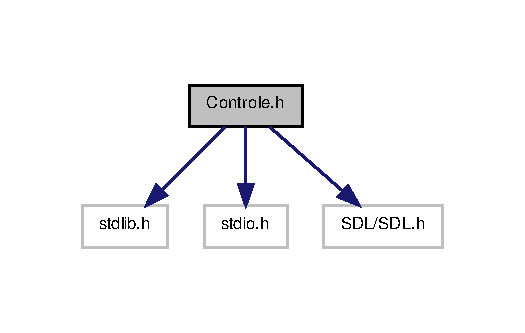
\includegraphics[width=276pt]{_controle_8h__incl}
\end{center}
\end{figure}
Ce graphe montre quels fichiers incluent directement ou indirectement ce fichier \-:\nopagebreak
\begin{figure}[H]
\begin{center}
\leavevmode
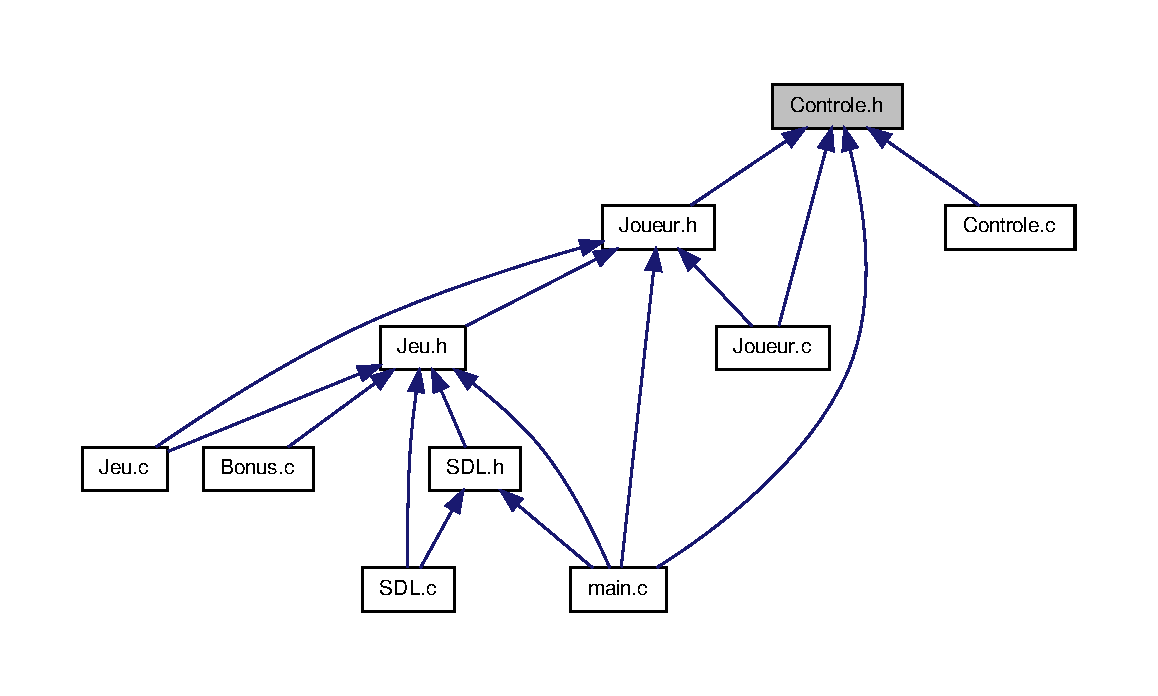
\includegraphics[width=350pt]{_controle_8h__dep__incl}
\end{center}
\end{figure}
\subsection*{Structures de données}
\begin{DoxyCompactItemize}
\item 
struct \hyperlink{struct_controle}{Controle}
\end{DoxyCompactItemize}
\subsection*{Fonctions}
\begin{DoxyCompactItemize}
\item 
S\-D\-L\-Key \hyperlink{_controle_8h_aceb59e2dc81ee481b6f4e4512451ca2c}{Controle\-Get\-Droite} (const \hyperlink{struct_controle}{Controle} $\ast$controle)
\item 
S\-D\-L\-Key \hyperlink{_controle_8h_a58b4a2d8f6f6248519b47d045d205144}{Controle\-Get\-Haut} (const \hyperlink{struct_controle}{Controle} $\ast$controle)
\item 
S\-D\-L\-Key \hyperlink{_controle_8h_afbc4a836ab3364317147c49c68071191}{Controle\-Get\-Bas} (const \hyperlink{struct_controle}{Controle} $\ast$controle)
\item 
S\-D\-L\-Key \hyperlink{_controle_8h_a2e052af3b9995a418ffae3f816068c40}{Controle\-Get\-Gauche} (const \hyperlink{struct_controle}{Controle} $\ast$controle)
\item 
S\-D\-L\-Key \hyperlink{_controle_8h_a777b3cf5baab32a2048abd6c334ee1cf}{Controle\-Get\-Bonus} (const \hyperlink{struct_controle}{Controle} $\ast$controle)
\item 
void \hyperlink{_controle_8h_ac551619cdc29f2173ec6a2b528793f20}{Controle\-Set\-Droite} (\hyperlink{struct_controle}{Controle} $\ast$controle, S\-D\-L\-Key x)
\item 
void \hyperlink{_controle_8h_afdede420fafbf282b46f799ae0bfcb4b}{Controle\-Set\-Haut} (\hyperlink{struct_controle}{Controle} $\ast$controle, S\-D\-L\-Key x)
\item 
void \hyperlink{_controle_8h_a9d8236e4578c1941fa13c7713bc1b9c2}{Controle\-Set\-Bas} (\hyperlink{struct_controle}{Controle} $\ast$controle, S\-D\-L\-Key x)
\item 
void \hyperlink{_controle_8h_a8d64b2f88ae1accc2fb58a7a394fe904}{Controle\-Set\-Gauche} (\hyperlink{struct_controle}{Controle} $\ast$controle, S\-D\-L\-Key x)
\item 
void \hyperlink{_controle_8h_a53dc76310eaee419e4d0d1b3d5e39003}{Controle\-Set\-Bonus} (\hyperlink{struct_controle}{Controle} $\ast$controle, S\-D\-L\-Key x)
\item 
void \hyperlink{_controle_8h_a3097aea62abd4e67f4c319756ad88a0e}{Controle\-Constructeur} (\hyperlink{struct_controle}{Controle} $\ast$controle, S\-D\-L\-Key haut, S\-D\-L\-Key bas, S\-D\-L\-Key gauche, S\-D\-L\-Key droite, S\-D\-L\-Key bonus)
\item 
void \hyperlink{_controle_8h_af1bb24fb9790dc018f7396c15e7b47a0}{Controle\-Destructeur} (\hyperlink{struct_controle}{Controle} $\ast$controle)
\item 
void \hyperlink{_controle_8h_a49d6667e80a116e40db1741c08616600}{Controle\-Test\-Regression} ()
\end{DoxyCompactItemize}


\subsection{Description détaillée}
\mbox{]} Module qui défini les Controles \begin{DoxyAuthor}{Auteur}
\{Antoine.\-C,Matthieu.\-B\} 
\end{DoxyAuthor}
\begin{DoxyVersion}{Version}
0.\-1 
\end{DoxyVersion}
\begin{DoxyDate}{Date}
13 mars 2013 
\end{DoxyDate}


Définition dans le fichier \hyperlink{_controle_8h_source}{Controle.\-h}.



\subsection{Documentation des fonctions}
\hypertarget{_controle_8h_a3097aea62abd4e67f4c319756ad88a0e}{\index{Controle.\-h@{Controle.\-h}!Controle\-Constructeur@{Controle\-Constructeur}}
\index{Controle\-Constructeur@{Controle\-Constructeur}!Controle.h@{Controle.\-h}}
\subsubsection[{Controle\-Constructeur}]{\setlength{\rightskip}{0pt plus 5cm}void Controle\-Constructeur (
\begin{DoxyParamCaption}
\item[{{\bf Controle} $\ast$}]{controle, }
\item[{S\-D\-L\-Key}]{haut, }
\item[{S\-D\-L\-Key}]{bas, }
\item[{S\-D\-L\-Key}]{gauche, }
\item[{S\-D\-L\-Key}]{droite, }
\item[{S\-D\-L\-Key}]{bonus}
\end{DoxyParamCaption}
)}}\label{_controle_8h_a3097aea62abd4e67f4c319756ad88a0e}


Définition à la ligne 49 du fichier Controle.\-c.

\hypertarget{_controle_8h_af1bb24fb9790dc018f7396c15e7b47a0}{\index{Controle.\-h@{Controle.\-h}!Controle\-Destructeur@{Controle\-Destructeur}}
\index{Controle\-Destructeur@{Controle\-Destructeur}!Controle.h@{Controle.\-h}}
\subsubsection[{Controle\-Destructeur}]{\setlength{\rightskip}{0pt plus 5cm}void Controle\-Destructeur (
\begin{DoxyParamCaption}
\item[{{\bf Controle} $\ast$}]{controle}
\end{DoxyParamCaption}
)}}\label{_controle_8h_af1bb24fb9790dc018f7396c15e7b47a0}


Définition à la ligne 57 du fichier Controle.\-c.

\hypertarget{_controle_8h_afbc4a836ab3364317147c49c68071191}{\index{Controle.\-h@{Controle.\-h}!Controle\-Get\-Bas@{Controle\-Get\-Bas}}
\index{Controle\-Get\-Bas@{Controle\-Get\-Bas}!Controle.h@{Controle.\-h}}
\subsubsection[{Controle\-Get\-Bas}]{\setlength{\rightskip}{0pt plus 5cm}S\-D\-L\-Key Controle\-Get\-Bas (
\begin{DoxyParamCaption}
\item[{const {\bf Controle} $\ast$}]{controle}
\end{DoxyParamCaption}
)}}\label{_controle_8h_afbc4a836ab3364317147c49c68071191}


Définition à la ligne 24 du fichier Controle.\-c.

\hypertarget{_controle_8h_a777b3cf5baab32a2048abd6c334ee1cf}{\index{Controle.\-h@{Controle.\-h}!Controle\-Get\-Bonus@{Controle\-Get\-Bonus}}
\index{Controle\-Get\-Bonus@{Controle\-Get\-Bonus}!Controle.h@{Controle.\-h}}
\subsubsection[{Controle\-Get\-Bonus}]{\setlength{\rightskip}{0pt plus 5cm}S\-D\-L\-Key Controle\-Get\-Bonus (
\begin{DoxyParamCaption}
\item[{const {\bf Controle} $\ast$}]{controle}
\end{DoxyParamCaption}
)}}\label{_controle_8h_a777b3cf5baab32a2048abd6c334ee1cf}


Définition à la ligne 28 du fichier Controle.\-c.

\hypertarget{_controle_8h_aceb59e2dc81ee481b6f4e4512451ca2c}{\index{Controle.\-h@{Controle.\-h}!Controle\-Get\-Droite@{Controle\-Get\-Droite}}
\index{Controle\-Get\-Droite@{Controle\-Get\-Droite}!Controle.h@{Controle.\-h}}
\subsubsection[{Controle\-Get\-Droite}]{\setlength{\rightskip}{0pt plus 5cm}S\-D\-L\-Key Controle\-Get\-Droite (
\begin{DoxyParamCaption}
\item[{const {\bf Controle} $\ast$}]{controle}
\end{DoxyParamCaption}
)}}\label{_controle_8h_aceb59e2dc81ee481b6f4e4512451ca2c}


Définition à la ligne 15 du fichier Controle.\-c.

\hypertarget{_controle_8h_a2e052af3b9995a418ffae3f816068c40}{\index{Controle.\-h@{Controle.\-h}!Controle\-Get\-Gauche@{Controle\-Get\-Gauche}}
\index{Controle\-Get\-Gauche@{Controle\-Get\-Gauche}!Controle.h@{Controle.\-h}}
\subsubsection[{Controle\-Get\-Gauche}]{\setlength{\rightskip}{0pt plus 5cm}S\-D\-L\-Key Controle\-Get\-Gauche (
\begin{DoxyParamCaption}
\item[{const {\bf Controle} $\ast$}]{controle}
\end{DoxyParamCaption}
)}}\label{_controle_8h_a2e052af3b9995a418ffae3f816068c40}


Définition à la ligne 21 du fichier Controle.\-c.

\hypertarget{_controle_8h_a58b4a2d8f6f6248519b47d045d205144}{\index{Controle.\-h@{Controle.\-h}!Controle\-Get\-Haut@{Controle\-Get\-Haut}}
\index{Controle\-Get\-Haut@{Controle\-Get\-Haut}!Controle.h@{Controle.\-h}}
\subsubsection[{Controle\-Get\-Haut}]{\setlength{\rightskip}{0pt plus 5cm}S\-D\-L\-Key Controle\-Get\-Haut (
\begin{DoxyParamCaption}
\item[{const {\bf Controle} $\ast$}]{controle}
\end{DoxyParamCaption}
)}}\label{_controle_8h_a58b4a2d8f6f6248519b47d045d205144}


Définition à la ligne 18 du fichier Controle.\-c.

\hypertarget{_controle_8h_a9d8236e4578c1941fa13c7713bc1b9c2}{\index{Controle.\-h@{Controle.\-h}!Controle\-Set\-Bas@{Controle\-Set\-Bas}}
\index{Controle\-Set\-Bas@{Controle\-Set\-Bas}!Controle.h@{Controle.\-h}}
\subsubsection[{Controle\-Set\-Bas}]{\setlength{\rightskip}{0pt plus 5cm}void Controle\-Set\-Bas (
\begin{DoxyParamCaption}
\item[{{\bf Controle} $\ast$}]{controle, }
\item[{S\-D\-L\-Key}]{x}
\end{DoxyParamCaption}
)}}\label{_controle_8h_a9d8236e4578c1941fa13c7713bc1b9c2}


Définition à la ligne 42 du fichier Controle.\-c.

\hypertarget{_controle_8h_a53dc76310eaee419e4d0d1b3d5e39003}{\index{Controle.\-h@{Controle.\-h}!Controle\-Set\-Bonus@{Controle\-Set\-Bonus}}
\index{Controle\-Set\-Bonus@{Controle\-Set\-Bonus}!Controle.h@{Controle.\-h}}
\subsubsection[{Controle\-Set\-Bonus}]{\setlength{\rightskip}{0pt plus 5cm}void Controle\-Set\-Bonus (
\begin{DoxyParamCaption}
\item[{{\bf Controle} $\ast$}]{controle, }
\item[{S\-D\-L\-Key}]{x}
\end{DoxyParamCaption}
)}}\label{_controle_8h_a53dc76310eaee419e4d0d1b3d5e39003}


Définition à la ligne 45 du fichier Controle.\-c.

\hypertarget{_controle_8h_ac551619cdc29f2173ec6a2b528793f20}{\index{Controle.\-h@{Controle.\-h}!Controle\-Set\-Droite@{Controle\-Set\-Droite}}
\index{Controle\-Set\-Droite@{Controle\-Set\-Droite}!Controle.h@{Controle.\-h}}
\subsubsection[{Controle\-Set\-Droite}]{\setlength{\rightskip}{0pt plus 5cm}void Controle\-Set\-Droite (
\begin{DoxyParamCaption}
\item[{{\bf Controle} $\ast$}]{controle, }
\item[{S\-D\-L\-Key}]{x}
\end{DoxyParamCaption}
)}}\label{_controle_8h_ac551619cdc29f2173ec6a2b528793f20}


Définition à la ligne 32 du fichier Controle.\-c.

\hypertarget{_controle_8h_a8d64b2f88ae1accc2fb58a7a394fe904}{\index{Controle.\-h@{Controle.\-h}!Controle\-Set\-Gauche@{Controle\-Set\-Gauche}}
\index{Controle\-Set\-Gauche@{Controle\-Set\-Gauche}!Controle.h@{Controle.\-h}}
\subsubsection[{Controle\-Set\-Gauche}]{\setlength{\rightskip}{0pt plus 5cm}void Controle\-Set\-Gauche (
\begin{DoxyParamCaption}
\item[{{\bf Controle} $\ast$}]{controle, }
\item[{S\-D\-L\-Key}]{x}
\end{DoxyParamCaption}
)}}\label{_controle_8h_a8d64b2f88ae1accc2fb58a7a394fe904}


Définition à la ligne 39 du fichier Controle.\-c.

\hypertarget{_controle_8h_afdede420fafbf282b46f799ae0bfcb4b}{\index{Controle.\-h@{Controle.\-h}!Controle\-Set\-Haut@{Controle\-Set\-Haut}}
\index{Controle\-Set\-Haut@{Controle\-Set\-Haut}!Controle.h@{Controle.\-h}}
\subsubsection[{Controle\-Set\-Haut}]{\setlength{\rightskip}{0pt plus 5cm}void Controle\-Set\-Haut (
\begin{DoxyParamCaption}
\item[{{\bf Controle} $\ast$}]{controle, }
\item[{S\-D\-L\-Key}]{x}
\end{DoxyParamCaption}
)}}\label{_controle_8h_afdede420fafbf282b46f799ae0bfcb4b}


Définition à la ligne 35 du fichier Controle.\-c.

\hypertarget{_controle_8h_a49d6667e80a116e40db1741c08616600}{\index{Controle.\-h@{Controle.\-h}!Controle\-Test\-Regression@{Controle\-Test\-Regression}}
\index{Controle\-Test\-Regression@{Controle\-Test\-Regression}!Controle.h@{Controle.\-h}}
\subsubsection[{Controle\-Test\-Regression}]{\setlength{\rightskip}{0pt plus 5cm}void Controle\-Test\-Regression (
\begin{DoxyParamCaption}
{}
\end{DoxyParamCaption}
)}}\label{_controle_8h_a49d6667e80a116e40db1741c08616600}


Définition à la ligne 66 du fichier Controle.\-c.


\hypertarget{_couleur_8h}{\section{Référence du fichier Couleur.\-h}
\label{_couleur_8h}\index{Couleur.\-h@{Couleur.\-h}}
}
Ce graphe montre quels fichiers incluent directement ou indirectement ce fichier \-:\nopagebreak
\begin{figure}[H]
\begin{center}
\leavevmode
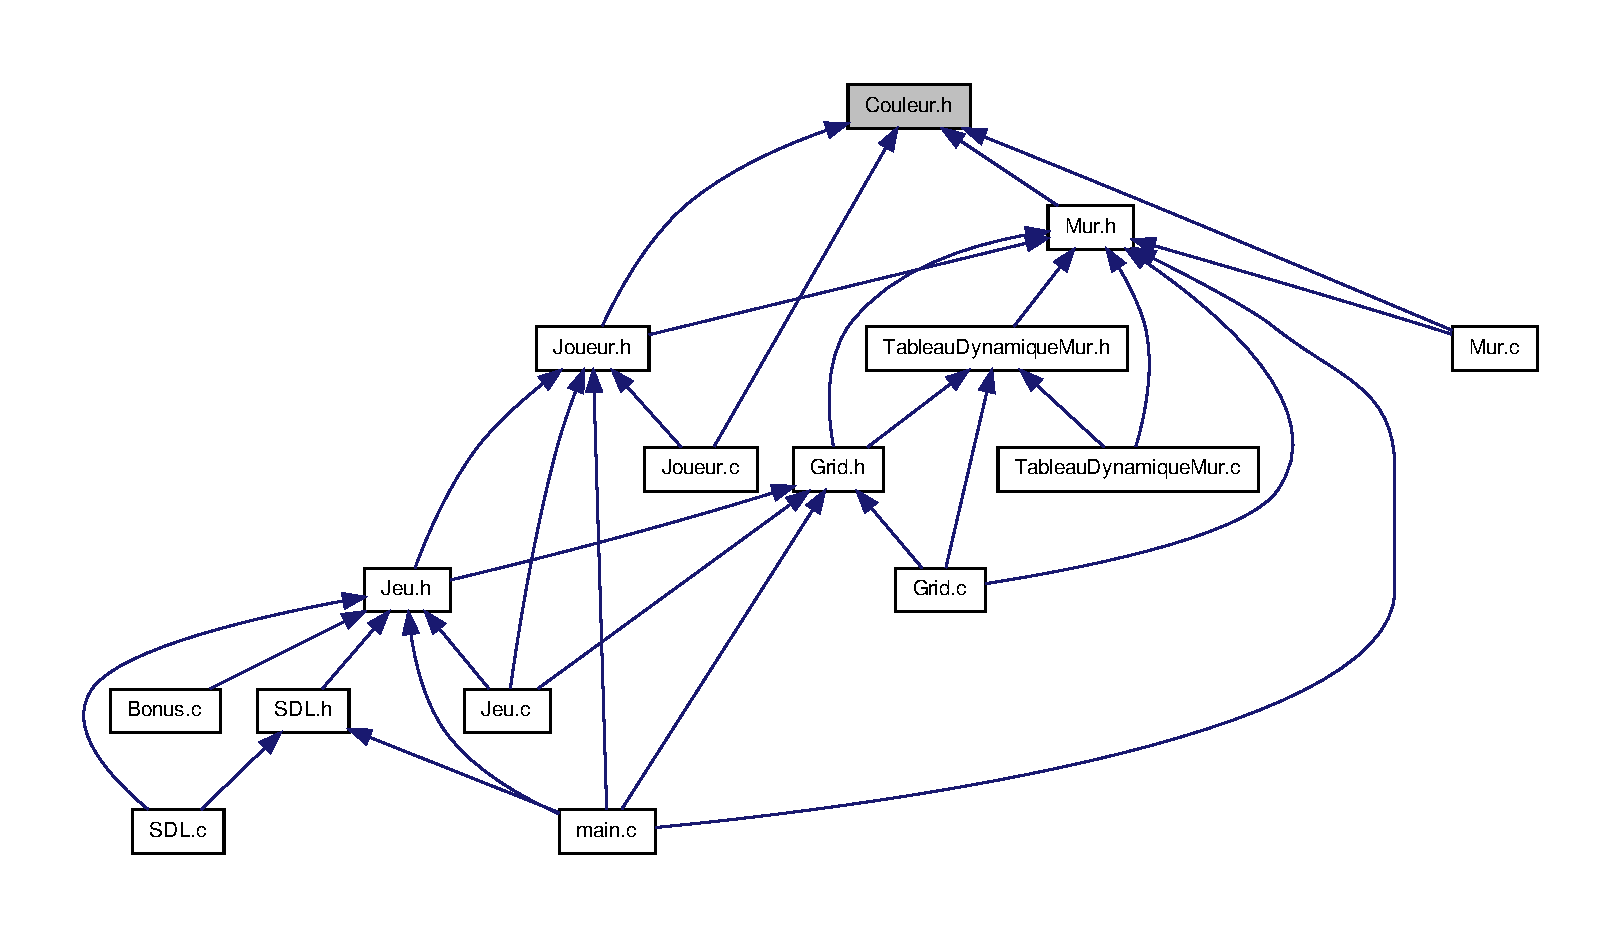
\includegraphics[width=217pt]{_couleur_8h__dep__incl}
\end{center}
\end{figure}
\subsection*{Énumérations}
\begin{DoxyCompactItemize}
\item 
enum \hyperlink{_couleur_8h_aa304d0ca681f782b1d7735da33037dd7}{Couleur} \{ \\*
\hyperlink{_couleur_8h_aa304d0ca681f782b1d7735da33037dd7a59e3323a198f0162330111165caaf367}{N\-O\-I\-R} =0, 
\hyperlink{_couleur_8h_aa304d0ca681f782b1d7735da33037dd7ace9ee4c1a6b777940c7f3a766a9a88d4}{O\-R\-A\-N\-G\-E} =1, 
\hyperlink{_couleur_8h_aa304d0ca681f782b1d7735da33037dd7a1b592b20aeb91b073f8f249231622230}{B\-L\-E\-U} =2, 
\hyperlink{_couleur_8h_aa304d0ca681f782b1d7735da33037dd7a92b33cebaccf73541ab06eca48a31e42}{R\-O\-U\-G\-E} =3, 
\\*
\hyperlink{_couleur_8h_aa304d0ca681f782b1d7735da33037dd7a14aeed4d25cc6ce52191b46c1d73af92}{V\-E\-R\-T} =4, 
\hyperlink{_couleur_8h_aa304d0ca681f782b1d7735da33037dd7a7088400e4fa72e2239115e7c0b294ea4}{V\-I\-O\-L\-E\-T} =5, 
\hyperlink{_couleur_8h_aa304d0ca681f782b1d7735da33037dd7aad89f3cf100d727ffd1e1aedb5bfbfd8}{B\-L\-E\-U\-F} =6, 
\hyperlink{_couleur_8h_aa304d0ca681f782b1d7735da33037dd7aeb840a0760d5c5122e980d507891c1a1}{J\-A\-U\-N\-E} =7, 
\\*
\hyperlink{_couleur_8h_aa304d0ca681f782b1d7735da33037dd7a35653913ced93d8199f0378ec538a0c7}{B\-L\-A\-N\-C} =8
 \}
\end{DoxyCompactItemize}


\subsection{Description détaillée}
\mbox{]} Module des ccouleurs du jeu \begin{DoxyAuthor}{Auteur}
\{Antoine.\-C,Matthieu.\-B\} 
\end{DoxyAuthor}
\begin{DoxyVersion}{Version}
0.\-1 
\end{DoxyVersion}
\begin{DoxyDate}{Date}
13 mars 2013 
\end{DoxyDate}


Définition dans le fichier \hyperlink{_couleur_8h_source}{Couleur.\-h}.



\subsection{Documentation du type de l'énumération}
\hypertarget{_couleur_8h_aa304d0ca681f782b1d7735da33037dd7}{\index{Couleur.\-h@{Couleur.\-h}!Couleur@{Couleur}}
\index{Couleur@{Couleur}!Couleur.h@{Couleur.\-h}}
\subsubsection[{Couleur}]{\setlength{\rightskip}{0pt plus 5cm}enum {\bf Couleur}}}\label{_couleur_8h_aa304d0ca681f782b1d7735da33037dd7}
\begin{Desc}
\item[Valeurs énumérées]\par
\begin{description}
\index{N\-O\-I\-R@{N\-O\-I\-R}!Couleur.\-h@{Couleur.\-h}}\index{Couleur.\-h@{Couleur.\-h}!N\-O\-I\-R@{N\-O\-I\-R}}\item[{\em 
\hypertarget{_couleur_8h_aa304d0ca681f782b1d7735da33037dd7a59e3323a198f0162330111165caaf367}{N\-O\-I\-R}\label{_couleur_8h_aa304d0ca681f782b1d7735da33037dd7a59e3323a198f0162330111165caaf367}
}]\index{O\-R\-A\-N\-G\-E@{O\-R\-A\-N\-G\-E}!Couleur.\-h@{Couleur.\-h}}\index{Couleur.\-h@{Couleur.\-h}!O\-R\-A\-N\-G\-E@{O\-R\-A\-N\-G\-E}}\item[{\em 
\hypertarget{_couleur_8h_aa304d0ca681f782b1d7735da33037dd7ace9ee4c1a6b777940c7f3a766a9a88d4}{O\-R\-A\-N\-G\-E}\label{_couleur_8h_aa304d0ca681f782b1d7735da33037dd7ace9ee4c1a6b777940c7f3a766a9a88d4}
}]\index{B\-L\-E\-U@{B\-L\-E\-U}!Couleur.\-h@{Couleur.\-h}}\index{Couleur.\-h@{Couleur.\-h}!B\-L\-E\-U@{B\-L\-E\-U}}\item[{\em 
\hypertarget{_couleur_8h_aa304d0ca681f782b1d7735da33037dd7a1b592b20aeb91b073f8f249231622230}{B\-L\-E\-U}\label{_couleur_8h_aa304d0ca681f782b1d7735da33037dd7a1b592b20aeb91b073f8f249231622230}
}]\index{R\-O\-U\-G\-E@{R\-O\-U\-G\-E}!Couleur.\-h@{Couleur.\-h}}\index{Couleur.\-h@{Couleur.\-h}!R\-O\-U\-G\-E@{R\-O\-U\-G\-E}}\item[{\em 
\hypertarget{_couleur_8h_aa304d0ca681f782b1d7735da33037dd7a92b33cebaccf73541ab06eca48a31e42}{R\-O\-U\-G\-E}\label{_couleur_8h_aa304d0ca681f782b1d7735da33037dd7a92b33cebaccf73541ab06eca48a31e42}
}]\index{V\-E\-R\-T@{V\-E\-R\-T}!Couleur.\-h@{Couleur.\-h}}\index{Couleur.\-h@{Couleur.\-h}!V\-E\-R\-T@{V\-E\-R\-T}}\item[{\em 
\hypertarget{_couleur_8h_aa304d0ca681f782b1d7735da33037dd7a14aeed4d25cc6ce52191b46c1d73af92}{V\-E\-R\-T}\label{_couleur_8h_aa304d0ca681f782b1d7735da33037dd7a14aeed4d25cc6ce52191b46c1d73af92}
}]\index{V\-I\-O\-L\-E\-T@{V\-I\-O\-L\-E\-T}!Couleur.\-h@{Couleur.\-h}}\index{Couleur.\-h@{Couleur.\-h}!V\-I\-O\-L\-E\-T@{V\-I\-O\-L\-E\-T}}\item[{\em 
\hypertarget{_couleur_8h_aa304d0ca681f782b1d7735da33037dd7a7088400e4fa72e2239115e7c0b294ea4}{V\-I\-O\-L\-E\-T}\label{_couleur_8h_aa304d0ca681f782b1d7735da33037dd7a7088400e4fa72e2239115e7c0b294ea4}
}]\index{B\-L\-E\-U\-F@{B\-L\-E\-U\-F}!Couleur.\-h@{Couleur.\-h}}\index{Couleur.\-h@{Couleur.\-h}!B\-L\-E\-U\-F@{B\-L\-E\-U\-F}}\item[{\em 
\hypertarget{_couleur_8h_aa304d0ca681f782b1d7735da33037dd7aad89f3cf100d727ffd1e1aedb5bfbfd8}{B\-L\-E\-U\-F}\label{_couleur_8h_aa304d0ca681f782b1d7735da33037dd7aad89f3cf100d727ffd1e1aedb5bfbfd8}
}]\index{J\-A\-U\-N\-E@{J\-A\-U\-N\-E}!Couleur.\-h@{Couleur.\-h}}\index{Couleur.\-h@{Couleur.\-h}!J\-A\-U\-N\-E@{J\-A\-U\-N\-E}}\item[{\em 
\hypertarget{_couleur_8h_aa304d0ca681f782b1d7735da33037dd7aeb840a0760d5c5122e980d507891c1a1}{J\-A\-U\-N\-E}\label{_couleur_8h_aa304d0ca681f782b1d7735da33037dd7aeb840a0760d5c5122e980d507891c1a1}
}]\index{B\-L\-A\-N\-C@{B\-L\-A\-N\-C}!Couleur.\-h@{Couleur.\-h}}\index{Couleur.\-h@{Couleur.\-h}!B\-L\-A\-N\-C@{B\-L\-A\-N\-C}}\item[{\em 
\hypertarget{_couleur_8h_aa304d0ca681f782b1d7735da33037dd7a35653913ced93d8199f0378ec538a0c7}{B\-L\-A\-N\-C}\label{_couleur_8h_aa304d0ca681f782b1d7735da33037dd7a35653913ced93d8199f0378ec538a0c7}
}]\end{description}
\end{Desc}


Définition à la ligne 15 du fichier Couleur.\-h.


\hypertarget{_effet_bonus_8h}{\section{Référence du fichier Effet\-Bonus.\-h}
\label{_effet_bonus_8h}\index{Effet\-Bonus.\-h@{Effet\-Bonus.\-h}}
}
Ce graphe montre quels fichiers incluent directement ou indirectement ce fichier \-:\nopagebreak
\begin{figure}[H]
\begin{center}
\leavevmode
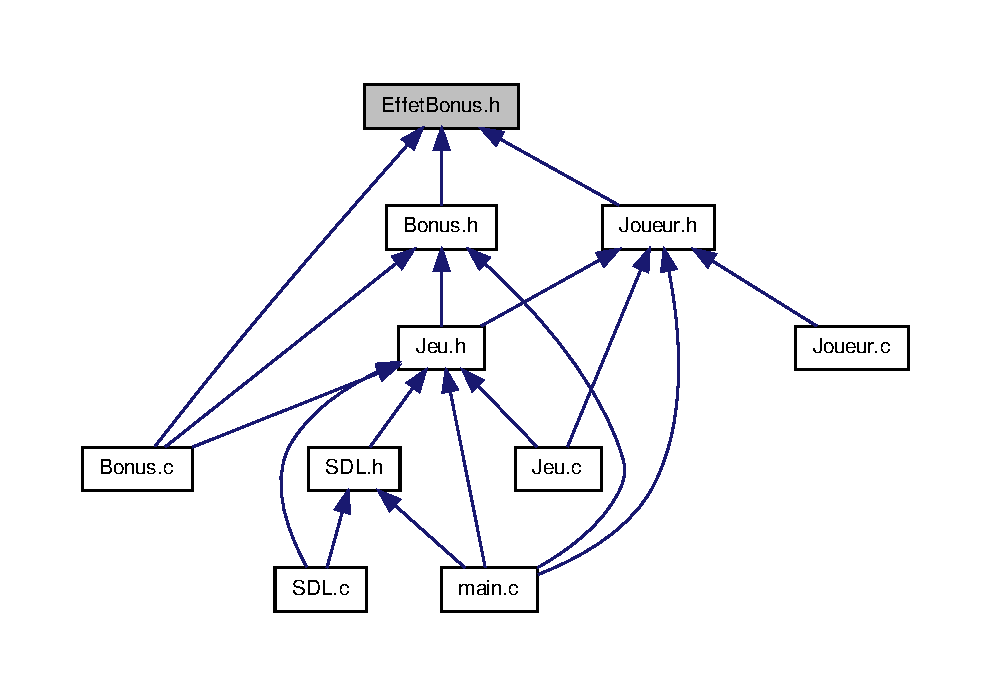
\includegraphics[width=350pt]{_effet_bonus_8h__dep__incl}
\end{center}
\end{figure}
\subsection*{Macros}
\begin{DoxyCompactItemize}
\item 
\#define \hyperlink{_effet_bonus_8h_ad1ded70ba9f4ccc722f58c14f4c63407}{\-\_\-\-Nombre\-\_\-\-Type\-\_\-\-Bonus}~2
\end{DoxyCompactItemize}
\subsection*{Énumérations}
\begin{DoxyCompactItemize}
\item 
enum \hyperlink{_effet_bonus_8h_a5c3ffd6a343fb8d5f63c87ee1a37a7fe}{Effet\-Bonus} \{ \hyperlink{_effet_bonus_8h_a5c3ffd6a343fb8d5f63c87ee1a37a7fea87797e00a316143a6c49ad311b240a2b}{A\-U\-C\-U\-N} =0, 
\hyperlink{_effet_bonus_8h_a5c3ffd6a343fb8d5f63c87ee1a37a7feac896e25bae3bb3d64b0200ec45e47ac5}{N\-E\-T\-T\-O\-Y\-A\-G\-E} =1, 
\hyperlink{_effet_bonus_8h_a5c3ffd6a343fb8d5f63c87ee1a37a7fea64fe15abfce0f5a1467d75dd876875ba}{B\-O\-O\-S\-T} =2
 \}
\end{DoxyCompactItemize}


\subsection{Description détaillée}
\mbox{]} Module des Motos du jeu \begin{DoxyAuthor}{Auteur}
\{Antoine.\-C,Matthieu.\-B\} 
\end{DoxyAuthor}
\begin{DoxyVersion}{Version}
1.\-1 
\end{DoxyVersion}
\begin{DoxyDate}{Date}
10 avril 2013 
\end{DoxyDate}


Définition dans le fichier \hyperlink{_effet_bonus_8h_source}{Effet\-Bonus.\-h}.



\subsection{Documentation des macros}
\hypertarget{_effet_bonus_8h_ad1ded70ba9f4ccc722f58c14f4c63407}{\index{Effet\-Bonus.\-h@{Effet\-Bonus.\-h}!\-\_\-\-Nombre\-\_\-\-Type\-\_\-\-Bonus@{\-\_\-\-Nombre\-\_\-\-Type\-\_\-\-Bonus}}
\index{\-\_\-\-Nombre\-\_\-\-Type\-\_\-\-Bonus@{\-\_\-\-Nombre\-\_\-\-Type\-\_\-\-Bonus}!EffetBonus.h@{Effet\-Bonus.\-h}}
\subsubsection[{\-\_\-\-Nombre\-\_\-\-Type\-\_\-\-Bonus}]{\setlength{\rightskip}{0pt plus 5cm}\#define \-\_\-\-Nombre\-\_\-\-Type\-\_\-\-Bonus~2}}\label{_effet_bonus_8h_ad1ded70ba9f4ccc722f58c14f4c63407}


Définition à la ligne 16 du fichier Effet\-Bonus.\-h.



\subsection{Documentation du type de l'énumération}
\hypertarget{_effet_bonus_8h_a5c3ffd6a343fb8d5f63c87ee1a37a7fe}{\index{Effet\-Bonus.\-h@{Effet\-Bonus.\-h}!Effet\-Bonus@{Effet\-Bonus}}
\index{Effet\-Bonus@{Effet\-Bonus}!EffetBonus.h@{Effet\-Bonus.\-h}}
\subsubsection[{Effet\-Bonus}]{\setlength{\rightskip}{0pt plus 5cm}enum {\bf Effet\-Bonus}}}\label{_effet_bonus_8h_a5c3ffd6a343fb8d5f63c87ee1a37a7fe}
\begin{Desc}
\item[Valeurs énumérées]\par
\begin{description}
\index{A\-U\-C\-U\-N@{A\-U\-C\-U\-N}!Effet\-Bonus.\-h@{Effet\-Bonus.\-h}}\index{Effet\-Bonus.\-h@{Effet\-Bonus.\-h}!A\-U\-C\-U\-N@{A\-U\-C\-U\-N}}\item[{\em 
\hypertarget{_effet_bonus_8h_a5c3ffd6a343fb8d5f63c87ee1a37a7fea87797e00a316143a6c49ad311b240a2b}{A\-U\-C\-U\-N}\label{_effet_bonus_8h_a5c3ffd6a343fb8d5f63c87ee1a37a7fea87797e00a316143a6c49ad311b240a2b}
}]\index{N\-E\-T\-T\-O\-Y\-A\-G\-E@{N\-E\-T\-T\-O\-Y\-A\-G\-E}!Effet\-Bonus.\-h@{Effet\-Bonus.\-h}}\index{Effet\-Bonus.\-h@{Effet\-Bonus.\-h}!N\-E\-T\-T\-O\-Y\-A\-G\-E@{N\-E\-T\-T\-O\-Y\-A\-G\-E}}\item[{\em 
\hypertarget{_effet_bonus_8h_a5c3ffd6a343fb8d5f63c87ee1a37a7feac896e25bae3bb3d64b0200ec45e47ac5}{N\-E\-T\-T\-O\-Y\-A\-G\-E}\label{_effet_bonus_8h_a5c3ffd6a343fb8d5f63c87ee1a37a7feac896e25bae3bb3d64b0200ec45e47ac5}
}]\index{B\-O\-O\-S\-T@{B\-O\-O\-S\-T}!Effet\-Bonus.\-h@{Effet\-Bonus.\-h}}\index{Effet\-Bonus.\-h@{Effet\-Bonus.\-h}!B\-O\-O\-S\-T@{B\-O\-O\-S\-T}}\item[{\em 
\hypertarget{_effet_bonus_8h_a5c3ffd6a343fb8d5f63c87ee1a37a7fea64fe15abfce0f5a1467d75dd876875ba}{B\-O\-O\-S\-T}\label{_effet_bonus_8h_a5c3ffd6a343fb8d5f63c87ee1a37a7fea64fe15abfce0f5a1467d75dd876875ba}
}]\end{description}
\end{Desc}


Définition à la ligne 15 du fichier Effet\-Bonus.\-h.


\hypertarget{_grid_8c}{\section{Référence du fichier Grid.\-c}
\label{_grid_8c}\index{Grid.\-c@{Grid.\-c}}
}
{\ttfamily \#include $<$stdlib.\-h$>$}\\*
{\ttfamily \#include $<$stdio.\-h$>$}\\*
{\ttfamily \#include $<$assert.\-h$>$}\\*
{\ttfamily \#include \char`\"{}Grid.\-h\char`\"{}}\\*
{\ttfamily \#include \char`\"{}Mur.\-h\char`\"{}}\\*
{\ttfamily \#include \char`\"{}Tableau\-Dynamique\-Mur.\-h\char`\"{}}\\*
Graphe des dépendances par inclusion de Grid.\-c\-:\nopagebreak
\begin{figure}[H]
\begin{center}
\leavevmode
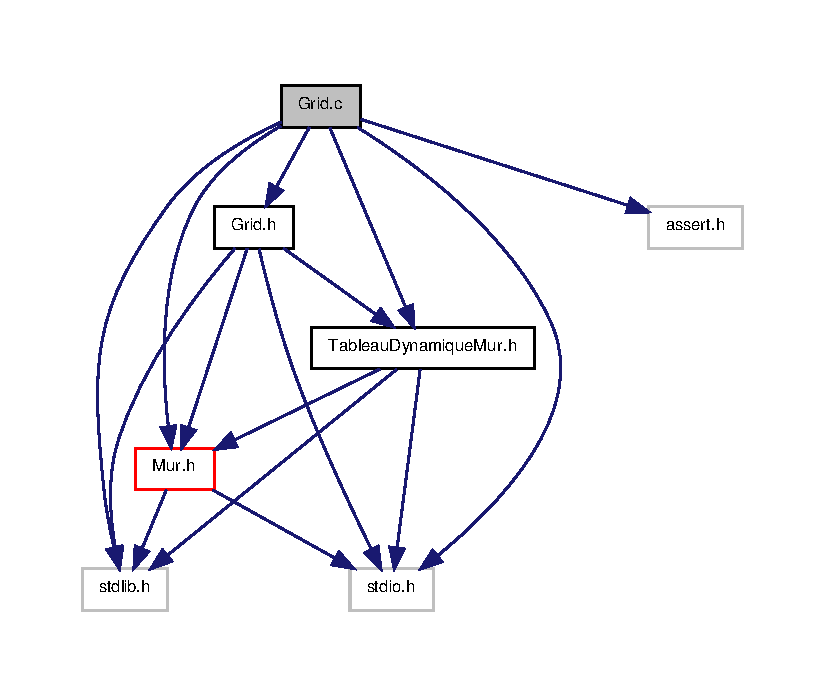
\includegraphics[width=350pt]{_grid_8c__incl}
\end{center}
\end{figure}
\subsection*{Fonctions}
\begin{DoxyCompactItemize}
\item 
float \hyperlink{_grid_8c_ad6474a4bd1b2abc33aed83f04ed4f0de}{Grid\-Get\-Position\-X} (const \hyperlink{struct_grid}{Grid} $\ast$grille)
\item 
float \hyperlink{_grid_8c_a7d16dec935d3ea2ea49a5ad80139ad63}{Grid\-Get\-Position\-Y} (const \hyperlink{struct_grid}{Grid} $\ast$grille)
\item 
unsigned int \hyperlink{_grid_8c_a402ec8dcb2070fdc1ca02d9f68b0d61f}{Grid\-Get\-Taille\-X} (const \hyperlink{struct_grid}{Grid} $\ast$grille)
\item 
unsigned int \hyperlink{_grid_8c_a6b28340c1a4dd9456ba5853963986cd2}{Grid\-Get\-Taille\-Y} (const \hyperlink{struct_grid}{Grid} $\ast$grille)
\item 
\hyperlink{struct_tableau_dynamique_mur}{Tableau\-Dynamique\-Mur} $\ast$ \hyperlink{_grid_8c_a1125c51c7a75905e5cf9322ac9b18bf0}{Grid\-Get\-Mes\-Murs} (\hyperlink{struct_grid}{Grid} $\ast$grille)
\item 
void \hyperlink{_grid_8c_a55dea47bf264d8c4c5f7ddf2584b3ec8}{Grid\-Set\-Position\-X} (\hyperlink{struct_grid}{Grid} $\ast$grille, float pos\-X)
\item 
void \hyperlink{_grid_8c_a1cdd44b889afbe59b178f6f256c4b32b}{Grid\-Set\-Position\-Y} (\hyperlink{struct_grid}{Grid} $\ast$grille, float pos\-Y)
\item 
void \hyperlink{_grid_8c_aa2af4ce645afe349bc5f7d448fa8d488}{Grid\-Set\-Taille\-X} (\hyperlink{struct_grid}{Grid} $\ast$grille, unsigned int taille\-X)
\item 
void \hyperlink{_grid_8c_a9778c91a23c761a7b0872611e24efc30}{Grid\-Set\-Taille\-Y} (\hyperlink{struct_grid}{Grid} $\ast$grille, unsigned int taille\-Y)
\item 
void \hyperlink{_grid_8c_ae58cdfa605fc9a0af1d8fa1461277bff}{Grid\-Set\-Mes\-Murs} (\hyperlink{struct_grid}{Grid} $\ast$grille, \hyperlink{struct_tableau_dynamique_mur}{Tableau\-Dynamique\-Mur} $\ast$mes\-Murs)
\item 
void \hyperlink{_grid_8c_a2cc97be9c7e6fc3a0fffa106c3cf8954}{Grid\-Constructeur} (\hyperlink{struct_grid}{Grid} $\ast$grille, float pos\-X, float pos\-Y, unsigned int Taille\-X, unsigned int Taille\-Y, \hyperlink{struct_tableau_dynamique_mur}{Tableau\-Dynamique\-Mur} $\ast$mes\-Murs)
\item 
void \hyperlink{_grid_8c_a5055e1bc05a5a03b8974301f64541ce5}{Grid\-Destructeur} (\hyperlink{struct_grid}{Grid} $\ast$grille)
\item 
void \hyperlink{_grid_8c_a7c5242962aa4ad47998bb4d04c4a3738}{ajoute\-Mur} (\hyperlink{struct_tableau_dynamique_mur}{Tableau\-Dynamique\-Mur} $\ast$mes\-Murs, \hyperlink{struct_mur}{Mur} mur)
\item 
void \hyperlink{_grid_8c_aa92f26b6a71343e3c05d7bf8fc218bb2}{efface\-Mur} (\hyperlink{struct_tableau_dynamique_mur}{Tableau\-Dynamique\-Mur} $\ast$mes\-Murs)
\item 
void \hyperlink{_grid_8c_a0e28e84d588ce2e55bbc743bb21c8731}{nettoie\-Grid} (\hyperlink{struct_tableau_dynamique_mur}{Tableau\-Dynamique\-Mur} $\ast$mes\-Murs)
\item 
void \hyperlink{_grid_8c_a84ff8aa0929298d2570fd909d90c7a17}{decremente\-Vie\-Mur} (\hyperlink{struct_grid}{Grid} $\ast$grille)
\item 
void \hyperlink{_grid_8c_aa9603343771db4d470b04bf9c3cf3fa4}{Grid\-Test\-Regression} ()
\end{DoxyCompactItemize}


\subsection{Description détaillée}
\mbox{]} Module des vecteurs \begin{DoxyAuthor}{Auteur}
\{Antoine.\-C,Matthieu.\-B\} 
\end{DoxyAuthor}
\begin{DoxyVersion}{Version}
1.\-0 
\end{DoxyVersion}
\begin{DoxyDate}{Date}
13 mars 2013 
\end{DoxyDate}


Définition dans le fichier \hyperlink{_grid_8c_source}{Grid.\-c}.



\subsection{Documentation des fonctions}
\hypertarget{_grid_8c_a7c5242962aa4ad47998bb4d04c4a3738}{\index{Grid.\-c@{Grid.\-c}!ajoute\-Mur@{ajoute\-Mur}}
\index{ajoute\-Mur@{ajoute\-Mur}!Grid.c@{Grid.\-c}}
\subsubsection[{ajoute\-Mur}]{\setlength{\rightskip}{0pt plus 5cm}void ajoute\-Mur (
\begin{DoxyParamCaption}
\item[{{\bf Tableau\-Dynamique\-Mur} $\ast$}]{mes\-Murs, }
\item[{{\bf Mur}}]{mur}
\end{DoxyParamCaption}
)}}\label{_grid_8c_a7c5242962aa4ad47998bb4d04c4a3738}


Définition à la ligne 63 du fichier Grid.\-c.

\hypertarget{_grid_8c_a84ff8aa0929298d2570fd909d90c7a17}{\index{Grid.\-c@{Grid.\-c}!decremente\-Vie\-Mur@{decremente\-Vie\-Mur}}
\index{decremente\-Vie\-Mur@{decremente\-Vie\-Mur}!Grid.c@{Grid.\-c}}
\subsubsection[{decremente\-Vie\-Mur}]{\setlength{\rightskip}{0pt plus 5cm}void decremente\-Vie\-Mur (
\begin{DoxyParamCaption}
\item[{{\bf Grid} $\ast$}]{grille}
\end{DoxyParamCaption}
)}}\label{_grid_8c_a84ff8aa0929298d2570fd909d90c7a17}


Définition à la ligne 80 du fichier Grid.\-c.

\hypertarget{_grid_8c_aa92f26b6a71343e3c05d7bf8fc218bb2}{\index{Grid.\-c@{Grid.\-c}!efface\-Mur@{efface\-Mur}}
\index{efface\-Mur@{efface\-Mur}!Grid.c@{Grid.\-c}}
\subsubsection[{efface\-Mur}]{\setlength{\rightskip}{0pt plus 5cm}void efface\-Mur (
\begin{DoxyParamCaption}
\item[{{\bf Tableau\-Dynamique\-Mur} $\ast$}]{mes\-Murs}
\end{DoxyParamCaption}
)}}\label{_grid_8c_aa92f26b6a71343e3c05d7bf8fc218bb2}


Définition à la ligne 67 du fichier Grid.\-c.

\hypertarget{_grid_8c_a2cc97be9c7e6fc3a0fffa106c3cf8954}{\index{Grid.\-c@{Grid.\-c}!Grid\-Constructeur@{Grid\-Constructeur}}
\index{Grid\-Constructeur@{Grid\-Constructeur}!Grid.c@{Grid.\-c}}
\subsubsection[{Grid\-Constructeur}]{\setlength{\rightskip}{0pt plus 5cm}void Grid\-Constructeur (
\begin{DoxyParamCaption}
\item[{{\bf Grid} $\ast$}]{grille, }
\item[{float}]{pos\-X, }
\item[{float}]{pos\-Y, }
\item[{unsigned int}]{Taille\-X, }
\item[{unsigned int}]{Taille\-Y, }
\item[{{\bf Tableau\-Dynamique\-Mur} $\ast$}]{mes\-Murs}
\end{DoxyParamCaption}
)}}\label{_grid_8c_a2cc97be9c7e6fc3a0fffa106c3cf8954}


Définition à la ligne 47 du fichier Grid.\-c.

\hypertarget{_grid_8c_a5055e1bc05a5a03b8974301f64541ce5}{\index{Grid.\-c@{Grid.\-c}!Grid\-Destructeur@{Grid\-Destructeur}}
\index{Grid\-Destructeur@{Grid\-Destructeur}!Grid.c@{Grid.\-c}}
\subsubsection[{Grid\-Destructeur}]{\setlength{\rightskip}{0pt plus 5cm}void Grid\-Destructeur (
\begin{DoxyParamCaption}
\item[{{\bf Grid} $\ast$}]{grille}
\end{DoxyParamCaption}
)}}\label{_grid_8c_a5055e1bc05a5a03b8974301f64541ce5}


Définition à la ligne 55 du fichier Grid.\-c.

\hypertarget{_grid_8c_a1125c51c7a75905e5cf9322ac9b18bf0}{\index{Grid.\-c@{Grid.\-c}!Grid\-Get\-Mes\-Murs@{Grid\-Get\-Mes\-Murs}}
\index{Grid\-Get\-Mes\-Murs@{Grid\-Get\-Mes\-Murs}!Grid.c@{Grid.\-c}}
\subsubsection[{Grid\-Get\-Mes\-Murs}]{\setlength{\rightskip}{0pt plus 5cm}{\bf Tableau\-Dynamique\-Mur}$\ast$ Grid\-Get\-Mes\-Murs (
\begin{DoxyParamCaption}
\item[{{\bf Grid} $\ast$}]{grille}
\end{DoxyParamCaption}
)}}\label{_grid_8c_a1125c51c7a75905e5cf9322ac9b18bf0}


Définition à la ligne 29 du fichier Grid.\-c.

\hypertarget{_grid_8c_ad6474a4bd1b2abc33aed83f04ed4f0de}{\index{Grid.\-c@{Grid.\-c}!Grid\-Get\-Position\-X@{Grid\-Get\-Position\-X}}
\index{Grid\-Get\-Position\-X@{Grid\-Get\-Position\-X}!Grid.c@{Grid.\-c}}
\subsubsection[{Grid\-Get\-Position\-X}]{\setlength{\rightskip}{0pt plus 5cm}float Grid\-Get\-Position\-X (
\begin{DoxyParamCaption}
\item[{const {\bf Grid} $\ast$}]{grille}
\end{DoxyParamCaption}
)}}\label{_grid_8c_ad6474a4bd1b2abc33aed83f04ed4f0de}


Définition à la ligne 17 du fichier Grid.\-c.

\hypertarget{_grid_8c_a7d16dec935d3ea2ea49a5ad80139ad63}{\index{Grid.\-c@{Grid.\-c}!Grid\-Get\-Position\-Y@{Grid\-Get\-Position\-Y}}
\index{Grid\-Get\-Position\-Y@{Grid\-Get\-Position\-Y}!Grid.c@{Grid.\-c}}
\subsubsection[{Grid\-Get\-Position\-Y}]{\setlength{\rightskip}{0pt plus 5cm}float Grid\-Get\-Position\-Y (
\begin{DoxyParamCaption}
\item[{const {\bf Grid} $\ast$}]{grille}
\end{DoxyParamCaption}
)}}\label{_grid_8c_a7d16dec935d3ea2ea49a5ad80139ad63}


Définition à la ligne 20 du fichier Grid.\-c.

\hypertarget{_grid_8c_a402ec8dcb2070fdc1ca02d9f68b0d61f}{\index{Grid.\-c@{Grid.\-c}!Grid\-Get\-Taille\-X@{Grid\-Get\-Taille\-X}}
\index{Grid\-Get\-Taille\-X@{Grid\-Get\-Taille\-X}!Grid.c@{Grid.\-c}}
\subsubsection[{Grid\-Get\-Taille\-X}]{\setlength{\rightskip}{0pt plus 5cm}unsigned int Grid\-Get\-Taille\-X (
\begin{DoxyParamCaption}
\item[{const {\bf Grid} $\ast$}]{grille}
\end{DoxyParamCaption}
)}}\label{_grid_8c_a402ec8dcb2070fdc1ca02d9f68b0d61f}


Définition à la ligne 23 du fichier Grid.\-c.

\hypertarget{_grid_8c_a6b28340c1a4dd9456ba5853963986cd2}{\index{Grid.\-c@{Grid.\-c}!Grid\-Get\-Taille\-Y@{Grid\-Get\-Taille\-Y}}
\index{Grid\-Get\-Taille\-Y@{Grid\-Get\-Taille\-Y}!Grid.c@{Grid.\-c}}
\subsubsection[{Grid\-Get\-Taille\-Y}]{\setlength{\rightskip}{0pt plus 5cm}unsigned int Grid\-Get\-Taille\-Y (
\begin{DoxyParamCaption}
\item[{const {\bf Grid} $\ast$}]{grille}
\end{DoxyParamCaption}
)}}\label{_grid_8c_a6b28340c1a4dd9456ba5853963986cd2}


Définition à la ligne 26 du fichier Grid.\-c.

\hypertarget{_grid_8c_ae58cdfa605fc9a0af1d8fa1461277bff}{\index{Grid.\-c@{Grid.\-c}!Grid\-Set\-Mes\-Murs@{Grid\-Set\-Mes\-Murs}}
\index{Grid\-Set\-Mes\-Murs@{Grid\-Set\-Mes\-Murs}!Grid.c@{Grid.\-c}}
\subsubsection[{Grid\-Set\-Mes\-Murs}]{\setlength{\rightskip}{0pt plus 5cm}void Grid\-Set\-Mes\-Murs (
\begin{DoxyParamCaption}
\item[{{\bf Grid} $\ast$}]{grille, }
\item[{{\bf Tableau\-Dynamique\-Mur} $\ast$}]{mes\-Murs}
\end{DoxyParamCaption}
)}}\label{_grid_8c_ae58cdfa605fc9a0af1d8fa1461277bff}


Définition à la ligne 44 du fichier Grid.\-c.

\hypertarget{_grid_8c_a55dea47bf264d8c4c5f7ddf2584b3ec8}{\index{Grid.\-c@{Grid.\-c}!Grid\-Set\-Position\-X@{Grid\-Set\-Position\-X}}
\index{Grid\-Set\-Position\-X@{Grid\-Set\-Position\-X}!Grid.c@{Grid.\-c}}
\subsubsection[{Grid\-Set\-Position\-X}]{\setlength{\rightskip}{0pt plus 5cm}void Grid\-Set\-Position\-X (
\begin{DoxyParamCaption}
\item[{{\bf Grid} $\ast$}]{grille, }
\item[{float}]{pos\-X}
\end{DoxyParamCaption}
)}}\label{_grid_8c_a55dea47bf264d8c4c5f7ddf2584b3ec8}


Définition à la ligne 32 du fichier Grid.\-c.

\hypertarget{_grid_8c_a1cdd44b889afbe59b178f6f256c4b32b}{\index{Grid.\-c@{Grid.\-c}!Grid\-Set\-Position\-Y@{Grid\-Set\-Position\-Y}}
\index{Grid\-Set\-Position\-Y@{Grid\-Set\-Position\-Y}!Grid.c@{Grid.\-c}}
\subsubsection[{Grid\-Set\-Position\-Y}]{\setlength{\rightskip}{0pt plus 5cm}void Grid\-Set\-Position\-Y (
\begin{DoxyParamCaption}
\item[{{\bf Grid} $\ast$}]{grille, }
\item[{float}]{pos\-Y}
\end{DoxyParamCaption}
)}}\label{_grid_8c_a1cdd44b889afbe59b178f6f256c4b32b}


Définition à la ligne 35 du fichier Grid.\-c.

\hypertarget{_grid_8c_aa2af4ce645afe349bc5f7d448fa8d488}{\index{Grid.\-c@{Grid.\-c}!Grid\-Set\-Taille\-X@{Grid\-Set\-Taille\-X}}
\index{Grid\-Set\-Taille\-X@{Grid\-Set\-Taille\-X}!Grid.c@{Grid.\-c}}
\subsubsection[{Grid\-Set\-Taille\-X}]{\setlength{\rightskip}{0pt plus 5cm}void Grid\-Set\-Taille\-X (
\begin{DoxyParamCaption}
\item[{{\bf Grid} $\ast$}]{grille, }
\item[{unsigned int}]{taille\-X}
\end{DoxyParamCaption}
)}}\label{_grid_8c_aa2af4ce645afe349bc5f7d448fa8d488}


Définition à la ligne 38 du fichier Grid.\-c.

\hypertarget{_grid_8c_a9778c91a23c761a7b0872611e24efc30}{\index{Grid.\-c@{Grid.\-c}!Grid\-Set\-Taille\-Y@{Grid\-Set\-Taille\-Y}}
\index{Grid\-Set\-Taille\-Y@{Grid\-Set\-Taille\-Y}!Grid.c@{Grid.\-c}}
\subsubsection[{Grid\-Set\-Taille\-Y}]{\setlength{\rightskip}{0pt plus 5cm}void Grid\-Set\-Taille\-Y (
\begin{DoxyParamCaption}
\item[{{\bf Grid} $\ast$}]{grille, }
\item[{unsigned int}]{taille\-Y}
\end{DoxyParamCaption}
)}}\label{_grid_8c_a9778c91a23c761a7b0872611e24efc30}


Définition à la ligne 41 du fichier Grid.\-c.

\hypertarget{_grid_8c_aa9603343771db4d470b04bf9c3cf3fa4}{\index{Grid.\-c@{Grid.\-c}!Grid\-Test\-Regression@{Grid\-Test\-Regression}}
\index{Grid\-Test\-Regression@{Grid\-Test\-Regression}!Grid.c@{Grid.\-c}}
\subsubsection[{Grid\-Test\-Regression}]{\setlength{\rightskip}{0pt plus 5cm}Grid\-Test\-Regression (
\begin{DoxyParamCaption}
{}
\end{DoxyParamCaption}
)}}\label{_grid_8c_aa9603343771db4d470b04bf9c3cf3fa4}
procédure de Test du module 

Définition à la ligne 94 du fichier Grid.\-c.

\hypertarget{_grid_8c_a0e28e84d588ce2e55bbc743bb21c8731}{\index{Grid.\-c@{Grid.\-c}!nettoie\-Grid@{nettoie\-Grid}}
\index{nettoie\-Grid@{nettoie\-Grid}!Grid.c@{Grid.\-c}}
\subsubsection[{nettoie\-Grid}]{\setlength{\rightskip}{0pt plus 5cm}void nettoie\-Grid (
\begin{DoxyParamCaption}
\item[{{\bf Tableau\-Dynamique\-Mur} $\ast$}]{mes\-Murs}
\end{DoxyParamCaption}
)}}\label{_grid_8c_a0e28e84d588ce2e55bbc743bb21c8731}


Définition à la ligne 76 du fichier Grid.\-c.


\hypertarget{_grid_8h}{\section{Référence du fichier Grid.\-h}
\label{_grid_8h}\index{Grid.\-h@{Grid.\-h}}
}
{\ttfamily \#include \char`\"{}Mur.\-h\char`\"{}}\\*
{\ttfamily \#include $<$stdlib.\-h$>$}\\*
{\ttfamily \#include $<$stdio.\-h$>$}\\*
{\ttfamily \#include \char`\"{}Tableau\-Dynamique\-Mur.\-h\char`\"{}}\\*
Graphe des dépendances par inclusion de Grid.\-h\-:\nopagebreak
\begin{figure}[H]
\begin{center}
\leavevmode
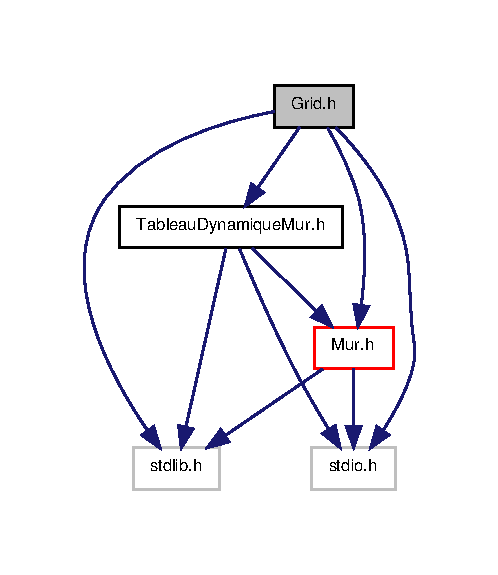
\includegraphics[width=239pt]{_grid_8h__incl}
\end{center}
\end{figure}
Ce graphe montre quels fichiers incluent directement ou indirectement ce fichier \-:\nopagebreak
\begin{figure}[H]
\begin{center}
\leavevmode
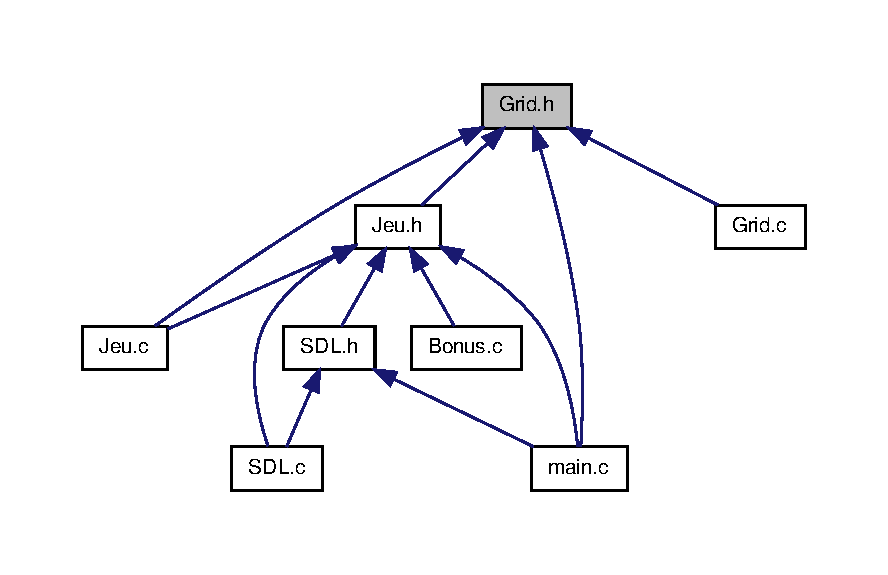
\includegraphics[width=246pt]{_grid_8h__dep__incl}
\end{center}
\end{figure}
\subsection*{Structures de données}
\begin{DoxyCompactItemize}
\item 
struct \hyperlink{struct_grid}{Grid}
\end{DoxyCompactItemize}
\subsection*{Fonctions}
\begin{DoxyCompactItemize}
\item 
float \hyperlink{_grid_8h_af3c58e084a35908474f7148cf177e717}{Grid\-Get\-Position\-X} (const \hyperlink{struct_grid}{Grid} $\ast$)
\item 
float \hyperlink{_grid_8h_a1763976e87177bc68c05b09e5efc0534}{Grid\-Get\-Position\-Y} (const \hyperlink{struct_grid}{Grid} $\ast$)
\item 
unsigned int \hyperlink{_grid_8h_ae4c0acd7634c52be99782403daf71f8e}{Grid\-Get\-Taille\-X} (const \hyperlink{struct_grid}{Grid} $\ast$)
\item 
unsigned int \hyperlink{_grid_8h_ab1b8157d42bd3763ead211ede9c667cc}{Grid\-Get\-Taille\-Y} (const \hyperlink{struct_grid}{Grid} $\ast$)
\item 
\hyperlink{struct_tableau_dynamique_mur}{Tableau\-Dynamique\-Mur} $\ast$ \hyperlink{_grid_8h_a90571a2b8569148c5adb00a0d1c8f78e}{Grid\-Get\-Mes\-Murs} (\hyperlink{struct_grid}{Grid} $\ast$)
\item 
void \hyperlink{_grid_8h_a55dea47bf264d8c4c5f7ddf2584b3ec8}{Grid\-Set\-Position\-X} (\hyperlink{struct_grid}{Grid} $\ast$grille, float pos\-X)
\item 
void \hyperlink{_grid_8h_a1cdd44b889afbe59b178f6f256c4b32b}{Grid\-Set\-Position\-Y} (\hyperlink{struct_grid}{Grid} $\ast$grille, float pos\-Y)
\item 
void \hyperlink{_grid_8h_a2f666baeec2f8712d60670e2ea196257}{Grid\-Set\-Taille\-X} (\hyperlink{struct_grid}{Grid} $\ast$, unsigned int)
\item 
void \hyperlink{_grid_8h_a7a7251a47cde9f4a26fd33145dab565f}{Grid\-Set\-Taille\-Y} (\hyperlink{struct_grid}{Grid} $\ast$, unsigned int)
\item 
void \hyperlink{_grid_8h_a707a4949087945113f1105e38449eaff}{Grid\-Set\-Mes\-Murs} (\hyperlink{struct_grid}{Grid} $\ast$, \hyperlink{struct_tableau_dynamique_mur}{Tableau\-Dynamique\-Mur} $\ast$)
\item 
void \hyperlink{_grid_8h_a214707008d196d1e43ba28528bfe7f95}{Grid\-Constructeur} (\hyperlink{struct_grid}{Grid} $\ast$, float, float, unsigned int, unsigned int, \hyperlink{struct_tableau_dynamique_mur}{Tableau\-Dynamique\-Mur} $\ast$)
\item 
void \hyperlink{_grid_8h_a5055e1bc05a5a03b8974301f64541ce5}{Grid\-Destructeur} (\hyperlink{struct_grid}{Grid} $\ast$grille)
\item 
void \hyperlink{_grid_8h_a7c5242962aa4ad47998bb4d04c4a3738}{ajoute\-Mur} (\hyperlink{struct_tableau_dynamique_mur}{Tableau\-Dynamique\-Mur} $\ast$mes\-Murs, \hyperlink{struct_mur}{Mur} mur)
\item 
void \hyperlink{_grid_8h_aa92f26b6a71343e3c05d7bf8fc218bb2}{efface\-Mur} (\hyperlink{struct_tableau_dynamique_mur}{Tableau\-Dynamique\-Mur} $\ast$mes\-Murs)
\item 
void \hyperlink{_grid_8h_a0e28e84d588ce2e55bbc743bb21c8731}{nettoie\-Grid} (\hyperlink{struct_tableau_dynamique_mur}{Tableau\-Dynamique\-Mur} $\ast$mes\-Murs)
\item 
void \hyperlink{_grid_8h_a84ff8aa0929298d2570fd909d90c7a17}{decremente\-Vie\-Mur} (\hyperlink{struct_grid}{Grid} $\ast$grille)
\item 
void \hyperlink{_grid_8h_a0c7fd37261e2118a2233698fb898f52a}{Grid\-Test\-Regression} ()
\end{DoxyCompactItemize}


\subsection{Description détaillée}
\mbox{]} Module des vecteurs \begin{DoxyAuthor}{Auteur}
\{Antoine.\-C,Matthieu.\-B\} 
\end{DoxyAuthor}
\begin{DoxyVersion}{Version}
0.\-1 
\end{DoxyVersion}
\begin{DoxyDate}{Date}
13 mars 2013 
\end{DoxyDate}


Définition dans le fichier \hyperlink{_grid_8h_source}{Grid.\-h}.



\subsection{Documentation des fonctions}
\hypertarget{_grid_8h_a7c5242962aa4ad47998bb4d04c4a3738}{\index{Grid.\-h@{Grid.\-h}!ajoute\-Mur@{ajoute\-Mur}}
\index{ajoute\-Mur@{ajoute\-Mur}!Grid.h@{Grid.\-h}}
\subsubsection[{ajoute\-Mur}]{\setlength{\rightskip}{0pt plus 5cm}void ajoute\-Mur (
\begin{DoxyParamCaption}
\item[{{\bf Tableau\-Dynamique\-Mur} $\ast$}]{mes\-Murs, }
\item[{{\bf Mur}}]{mur}
\end{DoxyParamCaption}
)}}\label{_grid_8h_a7c5242962aa4ad47998bb4d04c4a3738}


Définition à la ligne 63 du fichier Grid.\-c.

\hypertarget{_grid_8h_a84ff8aa0929298d2570fd909d90c7a17}{\index{Grid.\-h@{Grid.\-h}!decremente\-Vie\-Mur@{decremente\-Vie\-Mur}}
\index{decremente\-Vie\-Mur@{decremente\-Vie\-Mur}!Grid.h@{Grid.\-h}}
\subsubsection[{decremente\-Vie\-Mur}]{\setlength{\rightskip}{0pt plus 5cm}void decremente\-Vie\-Mur (
\begin{DoxyParamCaption}
\item[{{\bf Grid} $\ast$}]{grille}
\end{DoxyParamCaption}
)}}\label{_grid_8h_a84ff8aa0929298d2570fd909d90c7a17}


Définition à la ligne 80 du fichier Grid.\-c.

\hypertarget{_grid_8h_aa92f26b6a71343e3c05d7bf8fc218bb2}{\index{Grid.\-h@{Grid.\-h}!efface\-Mur@{efface\-Mur}}
\index{efface\-Mur@{efface\-Mur}!Grid.h@{Grid.\-h}}
\subsubsection[{efface\-Mur}]{\setlength{\rightskip}{0pt plus 5cm}void efface\-Mur (
\begin{DoxyParamCaption}
\item[{{\bf Tableau\-Dynamique\-Mur} $\ast$}]{mes\-Murs}
\end{DoxyParamCaption}
)}}\label{_grid_8h_aa92f26b6a71343e3c05d7bf8fc218bb2}


Définition à la ligne 67 du fichier Grid.\-c.

\hypertarget{_grid_8h_a214707008d196d1e43ba28528bfe7f95}{\index{Grid.\-h@{Grid.\-h}!Grid\-Constructeur@{Grid\-Constructeur}}
\index{Grid\-Constructeur@{Grid\-Constructeur}!Grid.h@{Grid.\-h}}
\subsubsection[{Grid\-Constructeur}]{\setlength{\rightskip}{0pt plus 5cm}void Grid\-Constructeur (
\begin{DoxyParamCaption}
\item[{{\bf Grid} $\ast$}]{, }
\item[{float}]{, }
\item[{float}]{, }
\item[{unsigned}]{int, }
\item[{unsigned}]{int, }
\item[{{\bf Tableau\-Dynamique\-Mur} $\ast$}]{}
\end{DoxyParamCaption}
)}}\label{_grid_8h_a214707008d196d1e43ba28528bfe7f95}


Définition à la ligne 47 du fichier Grid.\-c.

\hypertarget{_grid_8h_a5055e1bc05a5a03b8974301f64541ce5}{\index{Grid.\-h@{Grid.\-h}!Grid\-Destructeur@{Grid\-Destructeur}}
\index{Grid\-Destructeur@{Grid\-Destructeur}!Grid.h@{Grid.\-h}}
\subsubsection[{Grid\-Destructeur}]{\setlength{\rightskip}{0pt plus 5cm}void Grid\-Destructeur (
\begin{DoxyParamCaption}
\item[{{\bf Grid} $\ast$}]{grille}
\end{DoxyParamCaption}
)}}\label{_grid_8h_a5055e1bc05a5a03b8974301f64541ce5}


Définition à la ligne 55 du fichier Grid.\-c.

\hypertarget{_grid_8h_a90571a2b8569148c5adb00a0d1c8f78e}{\index{Grid.\-h@{Grid.\-h}!Grid\-Get\-Mes\-Murs@{Grid\-Get\-Mes\-Murs}}
\index{Grid\-Get\-Mes\-Murs@{Grid\-Get\-Mes\-Murs}!Grid.h@{Grid.\-h}}
\subsubsection[{Grid\-Get\-Mes\-Murs}]{\setlength{\rightskip}{0pt plus 5cm}{\bf Tableau\-Dynamique\-Mur}$\ast$ Grid\-Get\-Mes\-Murs (
\begin{DoxyParamCaption}
\item[{{\bf Grid} $\ast$}]{}
\end{DoxyParamCaption}
)}}\label{_grid_8h_a90571a2b8569148c5adb00a0d1c8f78e}


Définition à la ligne 29 du fichier Grid.\-c.

\hypertarget{_grid_8h_af3c58e084a35908474f7148cf177e717}{\index{Grid.\-h@{Grid.\-h}!Grid\-Get\-Position\-X@{Grid\-Get\-Position\-X}}
\index{Grid\-Get\-Position\-X@{Grid\-Get\-Position\-X}!Grid.h@{Grid.\-h}}
\subsubsection[{Grid\-Get\-Position\-X}]{\setlength{\rightskip}{0pt plus 5cm}float Grid\-Get\-Position\-X (
\begin{DoxyParamCaption}
\item[{const {\bf Grid} $\ast$}]{}
\end{DoxyParamCaption}
)}}\label{_grid_8h_af3c58e084a35908474f7148cf177e717}


Définition à la ligne 17 du fichier Grid.\-c.

\hypertarget{_grid_8h_a1763976e87177bc68c05b09e5efc0534}{\index{Grid.\-h@{Grid.\-h}!Grid\-Get\-Position\-Y@{Grid\-Get\-Position\-Y}}
\index{Grid\-Get\-Position\-Y@{Grid\-Get\-Position\-Y}!Grid.h@{Grid.\-h}}
\subsubsection[{Grid\-Get\-Position\-Y}]{\setlength{\rightskip}{0pt plus 5cm}float Grid\-Get\-Position\-Y (
\begin{DoxyParamCaption}
\item[{const {\bf Grid} $\ast$}]{}
\end{DoxyParamCaption}
)}}\label{_grid_8h_a1763976e87177bc68c05b09e5efc0534}


Définition à la ligne 20 du fichier Grid.\-c.

\hypertarget{_grid_8h_ae4c0acd7634c52be99782403daf71f8e}{\index{Grid.\-h@{Grid.\-h}!Grid\-Get\-Taille\-X@{Grid\-Get\-Taille\-X}}
\index{Grid\-Get\-Taille\-X@{Grid\-Get\-Taille\-X}!Grid.h@{Grid.\-h}}
\subsubsection[{Grid\-Get\-Taille\-X}]{\setlength{\rightskip}{0pt plus 5cm}unsigned int Grid\-Get\-Taille\-X (
\begin{DoxyParamCaption}
\item[{const {\bf Grid} $\ast$}]{}
\end{DoxyParamCaption}
)}}\label{_grid_8h_ae4c0acd7634c52be99782403daf71f8e}


Définition à la ligne 23 du fichier Grid.\-c.

\hypertarget{_grid_8h_ab1b8157d42bd3763ead211ede9c667cc}{\index{Grid.\-h@{Grid.\-h}!Grid\-Get\-Taille\-Y@{Grid\-Get\-Taille\-Y}}
\index{Grid\-Get\-Taille\-Y@{Grid\-Get\-Taille\-Y}!Grid.h@{Grid.\-h}}
\subsubsection[{Grid\-Get\-Taille\-Y}]{\setlength{\rightskip}{0pt plus 5cm}unsigned int Grid\-Get\-Taille\-Y (
\begin{DoxyParamCaption}
\item[{const {\bf Grid} $\ast$}]{}
\end{DoxyParamCaption}
)}}\label{_grid_8h_ab1b8157d42bd3763ead211ede9c667cc}


Définition à la ligne 26 du fichier Grid.\-c.

\hypertarget{_grid_8h_a707a4949087945113f1105e38449eaff}{\index{Grid.\-h@{Grid.\-h}!Grid\-Set\-Mes\-Murs@{Grid\-Set\-Mes\-Murs}}
\index{Grid\-Set\-Mes\-Murs@{Grid\-Set\-Mes\-Murs}!Grid.h@{Grid.\-h}}
\subsubsection[{Grid\-Set\-Mes\-Murs}]{\setlength{\rightskip}{0pt plus 5cm}void Grid\-Set\-Mes\-Murs (
\begin{DoxyParamCaption}
\item[{{\bf Grid} $\ast$}]{, }
\item[{{\bf Tableau\-Dynamique\-Mur} $\ast$}]{}
\end{DoxyParamCaption}
)}}\label{_grid_8h_a707a4949087945113f1105e38449eaff}


Définition à la ligne 44 du fichier Grid.\-c.

\hypertarget{_grid_8h_a55dea47bf264d8c4c5f7ddf2584b3ec8}{\index{Grid.\-h@{Grid.\-h}!Grid\-Set\-Position\-X@{Grid\-Set\-Position\-X}}
\index{Grid\-Set\-Position\-X@{Grid\-Set\-Position\-X}!Grid.h@{Grid.\-h}}
\subsubsection[{Grid\-Set\-Position\-X}]{\setlength{\rightskip}{0pt plus 5cm}void Grid\-Set\-Position\-X (
\begin{DoxyParamCaption}
\item[{{\bf Grid} $\ast$}]{grille, }
\item[{float}]{pos\-X}
\end{DoxyParamCaption}
)}}\label{_grid_8h_a55dea47bf264d8c4c5f7ddf2584b3ec8}


Définition à la ligne 32 du fichier Grid.\-c.

\hypertarget{_grid_8h_a1cdd44b889afbe59b178f6f256c4b32b}{\index{Grid.\-h@{Grid.\-h}!Grid\-Set\-Position\-Y@{Grid\-Set\-Position\-Y}}
\index{Grid\-Set\-Position\-Y@{Grid\-Set\-Position\-Y}!Grid.h@{Grid.\-h}}
\subsubsection[{Grid\-Set\-Position\-Y}]{\setlength{\rightskip}{0pt plus 5cm}void Grid\-Set\-Position\-Y (
\begin{DoxyParamCaption}
\item[{{\bf Grid} $\ast$}]{grille, }
\item[{float}]{pos\-Y}
\end{DoxyParamCaption}
)}}\label{_grid_8h_a1cdd44b889afbe59b178f6f256c4b32b}


Définition à la ligne 35 du fichier Grid.\-c.

\hypertarget{_grid_8h_a2f666baeec2f8712d60670e2ea196257}{\index{Grid.\-h@{Grid.\-h}!Grid\-Set\-Taille\-X@{Grid\-Set\-Taille\-X}}
\index{Grid\-Set\-Taille\-X@{Grid\-Set\-Taille\-X}!Grid.h@{Grid.\-h}}
\subsubsection[{Grid\-Set\-Taille\-X}]{\setlength{\rightskip}{0pt plus 5cm}void Grid\-Set\-Taille\-X (
\begin{DoxyParamCaption}
\item[{{\bf Grid} $\ast$}]{, }
\item[{unsigned}]{int}
\end{DoxyParamCaption}
)}}\label{_grid_8h_a2f666baeec2f8712d60670e2ea196257}


Définition à la ligne 38 du fichier Grid.\-c.

\hypertarget{_grid_8h_a7a7251a47cde9f4a26fd33145dab565f}{\index{Grid.\-h@{Grid.\-h}!Grid\-Set\-Taille\-Y@{Grid\-Set\-Taille\-Y}}
\index{Grid\-Set\-Taille\-Y@{Grid\-Set\-Taille\-Y}!Grid.h@{Grid.\-h}}
\subsubsection[{Grid\-Set\-Taille\-Y}]{\setlength{\rightskip}{0pt plus 5cm}void Grid\-Set\-Taille\-Y (
\begin{DoxyParamCaption}
\item[{{\bf Grid} $\ast$}]{, }
\item[{unsigned}]{int}
\end{DoxyParamCaption}
)}}\label{_grid_8h_a7a7251a47cde9f4a26fd33145dab565f}


Définition à la ligne 41 du fichier Grid.\-c.

\hypertarget{_grid_8h_a0c7fd37261e2118a2233698fb898f52a}{\index{Grid.\-h@{Grid.\-h}!Grid\-Test\-Regression@{Grid\-Test\-Regression}}
\index{Grid\-Test\-Regression@{Grid\-Test\-Regression}!Grid.h@{Grid.\-h}}
\subsubsection[{Grid\-Test\-Regression}]{\setlength{\rightskip}{0pt plus 5cm}void Grid\-Test\-Regression (
\begin{DoxyParamCaption}
{}
\end{DoxyParamCaption}
)}}\label{_grid_8h_a0c7fd37261e2118a2233698fb898f52a}
procédure de Test du module 

Définition à la ligne 94 du fichier Grid.\-c.

\hypertarget{_grid_8h_a0e28e84d588ce2e55bbc743bb21c8731}{\index{Grid.\-h@{Grid.\-h}!nettoie\-Grid@{nettoie\-Grid}}
\index{nettoie\-Grid@{nettoie\-Grid}!Grid.h@{Grid.\-h}}
\subsubsection[{nettoie\-Grid}]{\setlength{\rightskip}{0pt plus 5cm}void nettoie\-Grid (
\begin{DoxyParamCaption}
\item[{{\bf Tableau\-Dynamique\-Mur} $\ast$}]{mes\-Murs}
\end{DoxyParamCaption}
)}}\label{_grid_8h_a0e28e84d588ce2e55bbc743bb21c8731}


Définition à la ligne 76 du fichier Grid.\-c.


\hypertarget{_jeu_8c}{\section{Référence du fichier Jeu.\-c}
\label{_jeu_8c}\index{Jeu.\-c@{Jeu.\-c}}
}
{\ttfamily \#include \char`\"{}Jeu.\-h\char`\"{}}\\*
{\ttfamily \#include \char`\"{}Joueur.\-h\char`\"{}}\\*
{\ttfamily \#include \char`\"{}Grid.\-h\char`\"{}}\\*
{\ttfamily \#include $<$assert.\-h$>$}\\*
{\ttfamily \#include $<$math.\-h$>$}\\*
{\ttfamily \#include $<$stdio.\-h$>$}\\*
{\ttfamily \#include $<$stdlib.\-h$>$}\\*
{\ttfamily \#include $<$time.\-h$>$}\\*
{\ttfamily \#include \char`\"{}Tableau\-Dynamique\-Entier.\-h\char`\"{}}\\*
Graphe des dépendances par inclusion de Jeu.\-c\-:\nopagebreak
\begin{figure}[H]
\begin{center}
\leavevmode
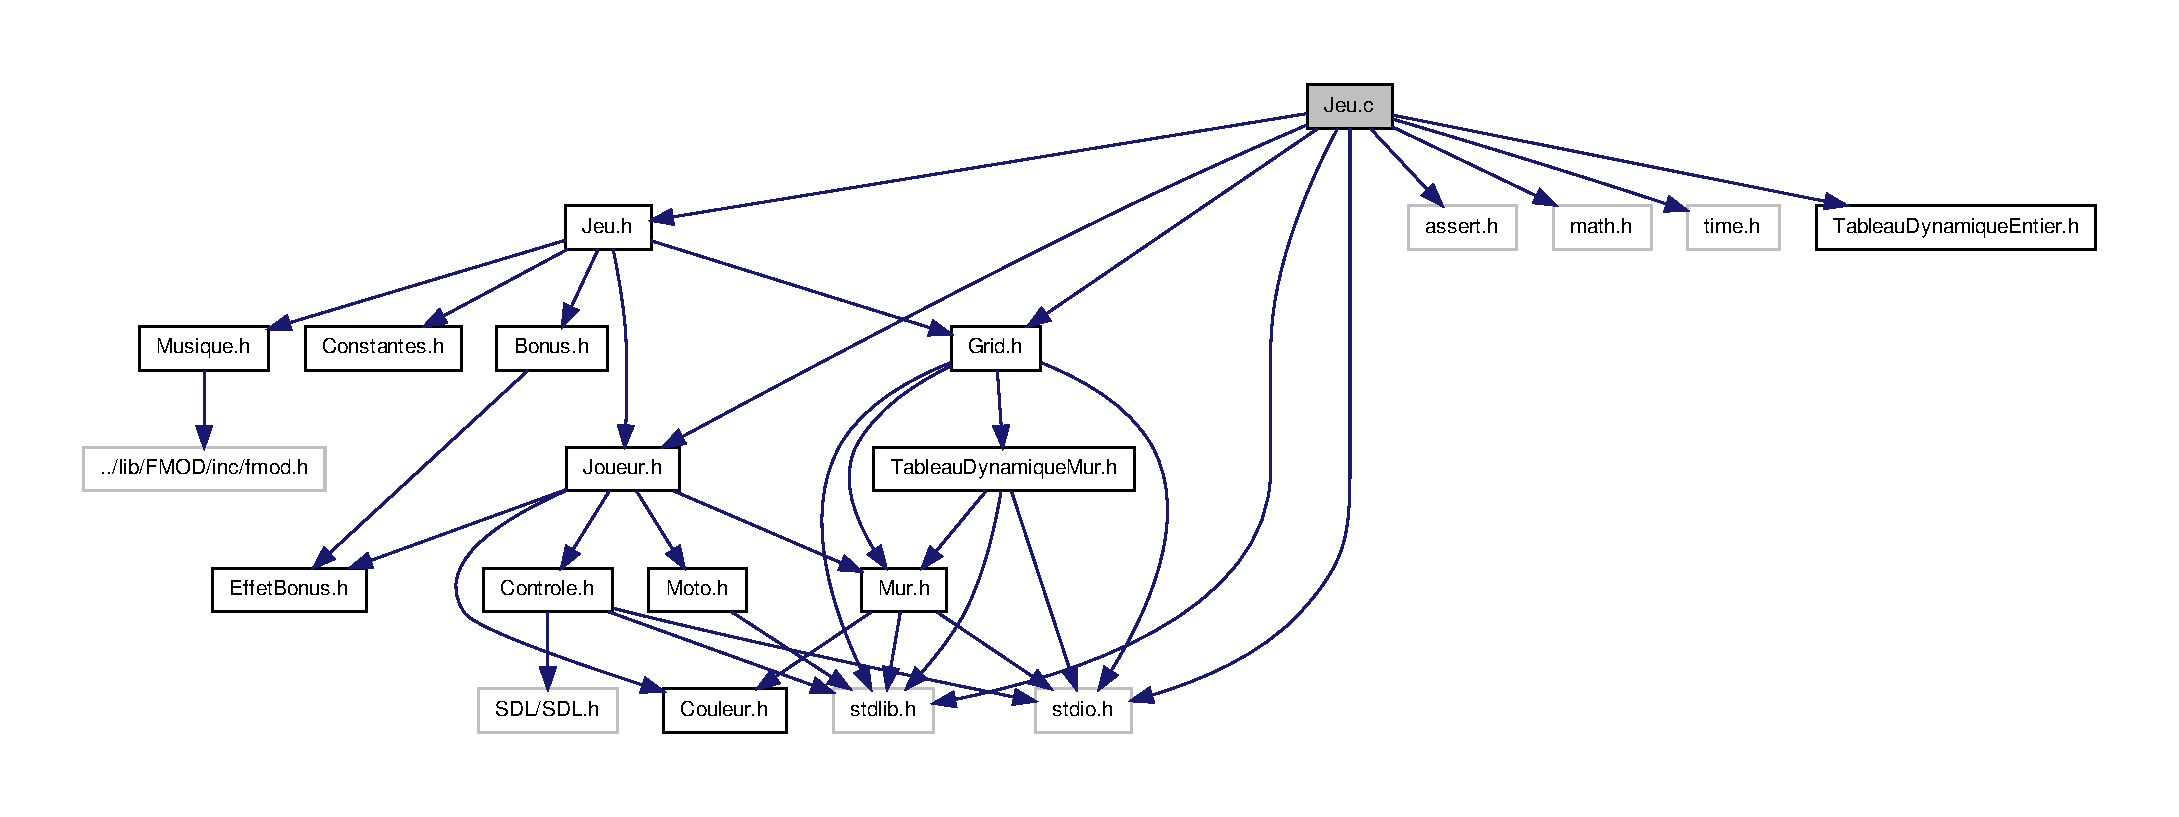
\includegraphics[width=350pt]{_jeu_8c__incl}
\end{center}
\end{figure}
\subsection*{Fonctions}
\begin{DoxyCompactItemize}
\item 
\hyperlink{struct_grid}{Grid} $\ast$ \hyperlink{_jeu_8c_a9cd710c657af64a74c7cc26a4e726d14}{Jeu\-Get\-Grille} (\hyperlink{struct_jeu}{Jeu} $\ast$jeu)
\item 
\hyperlink{struct_joueur}{Joueur} $\ast$ \hyperlink{_jeu_8c_a00cab8b79f7ac548749dd29b6a3dcefd}{Jeu\-Get\-Ieme\-Joueurs} (\hyperlink{struct_jeu}{Jeu} $\ast$jeu, int i)
\item 
int \hyperlink{_jeu_8c_a570c1b49959c5727b784ff980a9ca5ba}{Jeu\-Get\-Ieme\-Score} (\hyperlink{struct_jeu}{Jeu} $\ast$jeu, int i)
\item 
\hyperlink{struct_bonus}{Bonus} $\ast$ \hyperlink{_jeu_8c_a4d3ff47d4638c2a84807bc73b63c2040}{Jeu\-Get\-Ieme\-Bonus} (\hyperlink{struct_jeu}{Jeu} $\ast$jeu, int i)
\item 
int \hyperlink{_jeu_8c_ae4c5515bf7a3dc1b8c55dd193559cc59}{Jeu\-Get\-Temps\-Prochain\-Bonus} (\hyperlink{struct_jeu}{Jeu} $\ast$jeu)
\item 
\hyperlink{struct_musique}{Musique} $\ast$ \hyperlink{_jeu_8c_a960195d08a333a161de438fde3f0ce9c}{Jeu\-Get\-Musique} (\hyperlink{struct_jeu}{Jeu} $\ast$jeu)
\item 
void \hyperlink{_jeu_8c_a76c474e2d5c7de3fc3f4878346c33f6d}{Jeu\-Set\-Grille} (\hyperlink{struct_jeu}{Jeu} $\ast$jeu, \hyperlink{struct_grid}{Grid} $\ast$grille)
\item 
void \hyperlink{_jeu_8c_a5f97577deb2605062a4b7de1473aae9a}{Jeu\-Set\-Ieme\-Joueurs} (\hyperlink{struct_jeu}{Jeu} $\ast$jeu, \hyperlink{struct_joueur}{Joueur} $\ast$joueur, int i)
\item 
void \hyperlink{_jeu_8c_aed59312d10d85b62fbe0320d267c1172}{Jeu\-Set\-Ieme\-Score} (\hyperlink{struct_jeu}{Jeu} $\ast$jeu, int score, int i)
\item 
void \hyperlink{_jeu_8c_acd42a024bebfff90910b9694e6958531}{Jeu\-Set\-Ieme\-Bonus} (\hyperlink{struct_jeu}{Jeu} $\ast$jeu, const \hyperlink{struct_bonus}{Bonus} $\ast$bonus, int i)
\item 
void \hyperlink{_jeu_8c_a71ff5aea9bbf81e8ecd84a2a5a0d27cb}{Jeu\-Set\-Temps\-Prochain\-Bonus} (\hyperlink{struct_jeu}{Jeu} $\ast$jeu, int temps\-Prochain\-Bonus)
\item 
void \hyperlink{_jeu_8c_a21f6877d6b5377c9df2a8321313437f4}{Jeu\-Constructeur} (\hyperlink{struct_jeu}{Jeu} $\ast$jeu, \hyperlink{struct_grid}{Grid} $\ast$grille, \hyperlink{struct_joueur}{Joueur} $\ast$mes\-Joueurs, int $\ast$scores)
\item 
void \hyperlink{_jeu_8c_a8bcba1ef69f19fb2db2610e0391cfd51}{Jeu\-Destructeur} (\hyperlink{struct_jeu}{Jeu} $\ast$jeu)
\item 
char \hyperlink{_jeu_8c_ac2f5807a1e5457c87bad141d69a644ad}{test\-Collision\-Generique} (float objet1\mbox{[}4\mbox{]}, float objet2\mbox{[}4\mbox{]})
\item 
char \hyperlink{_jeu_8c_afc626a510d785dbffc9a7881229f0203}{test\-Collision\-Mur} (\hyperlink{struct_joueur}{Joueur} $\ast$joueur, \hyperlink{struct_grid}{Grid} $\ast$grille, char bool\-Saut)
\item 
char \hyperlink{_jeu_8c_a1d6d77911c3af96664c509572d7c9abe}{test\-Collision\-Moto} (\hyperlink{struct_moto}{Moto} $\ast$moto1, \hyperlink{struct_moto}{Moto} $\ast$moto2)
\item 
void \hyperlink{_jeu_8c_a43389b43f891711881d87d46c92a53a0}{Jeu\-Action\-Clavier} (\hyperlink{struct_joueur}{Joueur} $\ast$joueur, \hyperlink{_moto_8h_a224b9163917ac32fc95a60d8c1eec3aa}{Direction} direction, \hyperlink{struct_grid}{Grid} $\ast$grille)
\item 
void \hyperlink{_jeu_8c_ac2310df2f749aa58dc111b1bf906f2a8}{bouge\-Moto} (\hyperlink{struct_jeu}{Jeu} $\ast$jeu)
\item 
void \hyperlink{_jeu_8c_a71bdcf7116b2f14b792d222c49ff74de}{Jeu\-Evolue} (\hyperlink{struct_jeu}{Jeu} $\ast$jeu, short int $\ast$jeu\-Fini, char $\ast$nouveau\-Message, \hyperlink{_couleur_8h_aa304d0ca681f782b1d7735da33037dd7}{Couleur} $\ast$couleur\-Message)
\item 
void \hyperlink{_jeu_8c_acdb1470c32818255dca985898836aafa}{decremente\-Temps\-Bonus} (\hyperlink{struct_jeu}{Jeu} $\ast$jeu)
\item 
void \hyperlink{_jeu_8c_a2ce61226efe3fd99a225cb1609c14833}{Jeu\-Actionne\-Bonus} (\hyperlink{struct_joueur}{Joueur} $\ast$joueur)
\item 
char \hyperlink{_jeu_8c_a9045e76f8f81369ba40d35e5ca9b55ec}{test\-Collision\-Moto\-Bonus} (\hyperlink{struct_joueur}{Joueur} $\ast$mes\-Joueurs, \hyperlink{struct_bonus}{Bonus} $\ast$bonus)
\item 
void \hyperlink{_jeu_8c_a680716484ae925b266b97ed9cf1ca3be}{Place\-Bonus} (\hyperlink{struct_jeu}{Jeu} $\ast$jeu, \hyperlink{struct_bonus}{Bonus} $\ast$bonus)
\item 
void \hyperlink{_jeu_8c_aaa794bc48d4a68c8f3a3ffdb881f8eb3}{affiche\-Grille\-Analyse} (short int($\ast$grille\-Analyse)\mbox{[}\hyperlink{_constantes_8h_abf68bdf8402080e47166e730e6fa7839}{\-\_\-\-Taille\-\_\-\-Y\-\_\-\-Grille}/\hyperlink{_constantes_8h_a5486e43da0e415d8e657b6404134e6b7}{\-\_\-\-Precision\-\_\-\-Analyse\-\_\-\-I\-A}\mbox{]}\mbox{[}\hyperlink{_constantes_8h_a22ca4a20964744e6df65d2c81d5b41ff}{\-\_\-\-Taille\-\_\-\-X\-\_\-\-Grille}/\hyperlink{_constantes_8h_a5486e43da0e415d8e657b6404134e6b7}{\-\_\-\-Precision\-\_\-\-Analyse\-\_\-\-I\-A}\mbox{]})
\item 
void \hyperlink{_jeu_8c_a057ccaa58f66d1839542ce3ed73bd0d5}{affiche\-Grille\-Distances} (short int($\ast$grille\-Distance)\mbox{[}\hyperlink{_constantes_8h_abf68bdf8402080e47166e730e6fa7839}{\-\_\-\-Taille\-\_\-\-Y\-\_\-\-Grille}/\hyperlink{_constantes_8h_a5486e43da0e415d8e657b6404134e6b7}{\-\_\-\-Precision\-\_\-\-Analyse\-\_\-\-I\-A}\mbox{]}\mbox{[}\hyperlink{_constantes_8h_a22ca4a20964744e6df65d2c81d5b41ff}{\-\_\-\-Taille\-\_\-\-X\-\_\-\-Grille}/\hyperlink{_constantes_8h_a5486e43da0e415d8e657b6404134e6b7}{\-\_\-\-Precision\-\_\-\-Analyse\-\_\-\-I\-A}\mbox{]})
\item 
void \hyperlink{_jeu_8c_a7dadf0dab9b369d34f8db1e6f03220e4}{Jeu\-Gere\-I\-A} (\hyperlink{struct_joueur}{Joueur} $\ast$joueur\-I\-A, \hyperlink{struct_jeu}{Jeu} $\ast$jeu)
\item 
void \hyperlink{_jeu_8c_ae21534d3ce5552805c5c19c91835d45a}{indices\-Grille\-Joueur} (short int $\ast$ligne, short int $\ast$colonne, \hyperlink{struct_joueur}{Joueur} $\ast$joueur)
\item 
void \hyperlink{_jeu_8c_a935de1505ff299257332d32d9b450aaa}{creer\-Grille\-Distances} (short int ligne1, short int colonne1, short int($\ast$grille\-Analyse)\mbox{[}\hyperlink{_constantes_8h_abf68bdf8402080e47166e730e6fa7839}{\-\_\-\-Taille\-\_\-\-Y\-\_\-\-Grille}/\hyperlink{_constantes_8h_a5486e43da0e415d8e657b6404134e6b7}{\-\_\-\-Precision\-\_\-\-Analyse\-\_\-\-I\-A}\mbox{]}\mbox{[}\hyperlink{_constantes_8h_a22ca4a20964744e6df65d2c81d5b41ff}{\-\_\-\-Taille\-\_\-\-X\-\_\-\-Grille}/\hyperlink{_constantes_8h_a5486e43da0e415d8e657b6404134e6b7}{\-\_\-\-Precision\-\_\-\-Analyse\-\_\-\-I\-A}\mbox{]}, short int($\ast$grille\-Distance)\mbox{[}\hyperlink{_constantes_8h_abf68bdf8402080e47166e730e6fa7839}{\-\_\-\-Taille\-\_\-\-Y\-\_\-\-Grille}/\hyperlink{_constantes_8h_a5486e43da0e415d8e657b6404134e6b7}{\-\_\-\-Precision\-\_\-\-Analyse\-\_\-\-I\-A}\mbox{]}\mbox{[}\hyperlink{_constantes_8h_a22ca4a20964744e6df65d2c81d5b41ff}{\-\_\-\-Taille\-\_\-\-X\-\_\-\-Grille}/\hyperlink{_constantes_8h_a5486e43da0e415d8e657b6404134e6b7}{\-\_\-\-Precision\-\_\-\-Analyse\-\_\-\-I\-A}\mbox{]})
\item 
void \hyperlink{_jeu_8c_a3b3af5966cdc7cbf24276b5e80bdc032}{creer\-Grille\-Analyse} (short int($\ast$grille\-Analyse)\mbox{[}\hyperlink{_constantes_8h_abf68bdf8402080e47166e730e6fa7839}{\-\_\-\-Taille\-\_\-\-Y\-\_\-\-Grille}/\hyperlink{_constantes_8h_a5486e43da0e415d8e657b6404134e6b7}{\-\_\-\-Precision\-\_\-\-Analyse\-\_\-\-I\-A}\mbox{]}\mbox{[}\hyperlink{_constantes_8h_a22ca4a20964744e6df65d2c81d5b41ff}{\-\_\-\-Taille\-\_\-\-X\-\_\-\-Grille}/\hyperlink{_constantes_8h_a5486e43da0e415d8e657b6404134e6b7}{\-\_\-\-Precision\-\_\-\-Analyse\-\_\-\-I\-A}\mbox{]}, \hyperlink{struct_jeu}{Jeu} $\ast$jeu, \hyperlink{struct_joueur}{Joueur} $\ast$joueur\-I\-A)
\item 
short int \hyperlink{_jeu_8c_a8f806829e6634cfacfd7c54648baf3c6}{choisie\-Cible\-I\-A} (\hyperlink{struct_joueur}{Joueur} $\ast$joueur\-I\-A, \hyperlink{struct_jeu}{Jeu} $\ast$jeu, short int($\ast$grille\-Distance)\mbox{[}\hyperlink{_constantes_8h_abf68bdf8402080e47166e730e6fa7839}{\-\_\-\-Taille\-\_\-\-Y\-\_\-\-Grille}/\hyperlink{_constantes_8h_a5486e43da0e415d8e657b6404134e6b7}{\-\_\-\-Precision\-\_\-\-Analyse\-\_\-\-I\-A}\mbox{]}\mbox{[}\hyperlink{_constantes_8h_a22ca4a20964744e6df65d2c81d5b41ff}{\-\_\-\-Taille\-\_\-\-X\-\_\-\-Grille}/\hyperlink{_constantes_8h_a5486e43da0e415d8e657b6404134e6b7}{\-\_\-\-Precision\-\_\-\-Analyse\-\_\-\-I\-A}\mbox{]})
\item 
void \hyperlink{_jeu_8c_a234255b8c79dacdf45153d250a32cee5}{choisie\-Direction} (\hyperlink{struct_joueur}{Joueur} $\ast$joueur\-I\-A, \hyperlink{struct_jeu}{Jeu} $\ast$jeu, short int distance\-Joueur\-Cible, short int($\ast$grille\-Distance)\mbox{[}\hyperlink{_constantes_8h_abf68bdf8402080e47166e730e6fa7839}{\-\_\-\-Taille\-\_\-\-Y\-\_\-\-Grille}/\hyperlink{_constantes_8h_a5486e43da0e415d8e657b6404134e6b7}{\-\_\-\-Precision\-\_\-\-Analyse\-\_\-\-I\-A}\mbox{]}\mbox{[}\hyperlink{_constantes_8h_a22ca4a20964744e6df65d2c81d5b41ff}{\-\_\-\-Taille\-\_\-\-X\-\_\-\-Grille}/\hyperlink{_constantes_8h_a5486e43da0e415d8e657b6404134e6b7}{\-\_\-\-Precision\-\_\-\-Analyse\-\_\-\-I\-A}\mbox{]})
\item 
void \hyperlink{_jeu_8c_ab00a82316a8da0ba7425cb30e7b34b9f}{Jeu\-Test\-Regression} ()
\end{DoxyCompactItemize}


\subsection{Description détaillée}
\mbox{]} Module centrale du \hyperlink{struct_jeu}{Jeu} \begin{DoxyAuthor}{Auteur}
\{Antoine.\-C,Matthieu.\-B\} 
\end{DoxyAuthor}
\begin{DoxyVersion}{Version}
2.\-1 
\end{DoxyVersion}
\begin{DoxyDate}{Date}
13 mars 2013 
\end{DoxyDate}


Définition dans le fichier \hyperlink{_jeu_8c_source}{Jeu.\-c}.



\subsection{Documentation des fonctions}
\hypertarget{_jeu_8c_aaa794bc48d4a68c8f3a3ffdb881f8eb3}{\index{Jeu.\-c@{Jeu.\-c}!affiche\-Grille\-Analyse@{affiche\-Grille\-Analyse}}
\index{affiche\-Grille\-Analyse@{affiche\-Grille\-Analyse}!Jeu.c@{Jeu.\-c}}
\subsubsection[{affiche\-Grille\-Analyse}]{\setlength{\rightskip}{0pt plus 5cm}void affiche\-Grille\-Analyse (
\begin{DoxyParamCaption}
\item[{short int($\ast$)}]{grille\-Analyse\mbox{[}\-\_\-\-Taille\-\_\-\-Y\-\_\-\-Grille/\-\_\-\-Precision\-\_\-\-Analyse\-\_\-\-I\-A\mbox{]}\mbox{[}\-\_\-\-Taille\-\_\-\-X\-\_\-\-Grille/\-\_\-\-Precision\-\_\-\-Analyse\-\_\-\-I\-A\mbox{]}}
\end{DoxyParamCaption}
)}}\label{_jeu_8c_aaa794bc48d4a68c8f3a3ffdb881f8eb3}


Définition à la ligne 514 du fichier Jeu.\-c.

\hypertarget{_jeu_8c_a057ccaa58f66d1839542ce3ed73bd0d5}{\index{Jeu.\-c@{Jeu.\-c}!affiche\-Grille\-Distances@{affiche\-Grille\-Distances}}
\index{affiche\-Grille\-Distances@{affiche\-Grille\-Distances}!Jeu.c@{Jeu.\-c}}
\subsubsection[{affiche\-Grille\-Distances}]{\setlength{\rightskip}{0pt plus 5cm}void affiche\-Grille\-Distances (
\begin{DoxyParamCaption}
\item[{short int($\ast$)}]{grille\-Distance\mbox{[}\-\_\-\-Taille\-\_\-\-Y\-\_\-\-Grille/\-\_\-\-Precision\-\_\-\-Analyse\-\_\-\-I\-A\mbox{]}\mbox{[}\-\_\-\-Taille\-\_\-\-X\-\_\-\-Grille/\-\_\-\-Precision\-\_\-\-Analyse\-\_\-\-I\-A\mbox{]}}
\end{DoxyParamCaption}
)}}\label{_jeu_8c_a057ccaa58f66d1839542ce3ed73bd0d5}


Définition à la ligne 527 du fichier Jeu.\-c.

\hypertarget{_jeu_8c_ac2310df2f749aa58dc111b1bf906f2a8}{\index{Jeu.\-c@{Jeu.\-c}!bouge\-Moto@{bouge\-Moto}}
\index{bouge\-Moto@{bouge\-Moto}!Jeu.c@{Jeu.\-c}}
\subsubsection[{bouge\-Moto}]{\setlength{\rightskip}{0pt plus 5cm}void bouge\-Moto (
\begin{DoxyParamCaption}
\item[{{\bf Jeu} $\ast$}]{jeu}
\end{DoxyParamCaption}
)}}\label{_jeu_8c_ac2310df2f749aa58dc111b1bf906f2a8}


Définition à la ligne 232 du fichier Jeu.\-c.

\hypertarget{_jeu_8c_a8f806829e6634cfacfd7c54648baf3c6}{\index{Jeu.\-c@{Jeu.\-c}!choisie\-Cible\-I\-A@{choisie\-Cible\-I\-A}}
\index{choisie\-Cible\-I\-A@{choisie\-Cible\-I\-A}!Jeu.c@{Jeu.\-c}}
\subsubsection[{choisie\-Cible\-I\-A}]{\setlength{\rightskip}{0pt plus 5cm}short int choisie\-Cible\-I\-A (
\begin{DoxyParamCaption}
\item[{{\bf Joueur} $\ast$}]{joueur\-I\-A, }
\item[{{\bf Jeu} $\ast$}]{jeu, }
\item[{short int($\ast$)}]{grille\-Distance\mbox{[}\-\_\-\-Taille\-\_\-\-Y\-\_\-\-Grille/\-\_\-\-Precision\-\_\-\-Analyse\-\_\-\-I\-A\mbox{]}\mbox{[}\-\_\-\-Taille\-\_\-\-X\-\_\-\-Grille/\-\_\-\-Precision\-\_\-\-Analyse\-\_\-\-I\-A\mbox{]}}
\end{DoxyParamCaption}
)}}\label{_jeu_8c_a8f806829e6634cfacfd7c54648baf3c6}
!$<$On prend pour position du joueur le devant de sa moto Si cette case est inaccessible on prend une case plus loin 

Définition à la ligne 717 du fichier Jeu.\-c.

\hypertarget{_jeu_8c_a234255b8c79dacdf45153d250a32cee5}{\index{Jeu.\-c@{Jeu.\-c}!choisie\-Direction@{choisie\-Direction}}
\index{choisie\-Direction@{choisie\-Direction}!Jeu.c@{Jeu.\-c}}
\subsubsection[{choisie\-Direction}]{\setlength{\rightskip}{0pt plus 5cm}void choisie\-Direction (
\begin{DoxyParamCaption}
\item[{{\bf Joueur} $\ast$}]{joueur\-I\-A, }
\item[{{\bf Jeu} $\ast$}]{jeu, }
\item[{short int}]{distance\-Joueur\-Cible, }
\item[{short int($\ast$)}]{grille\-Distance\mbox{[}\-\_\-\-Taille\-\_\-\-Y\-\_\-\-Grille/\-\_\-\-Precision\-\_\-\-Analyse\-\_\-\-I\-A\mbox{]}\mbox{[}\-\_\-\-Taille\-\_\-\-X\-\_\-\-Grille/\-\_\-\-Precision\-\_\-\-Analyse\-\_\-\-I\-A\mbox{]}}
\end{DoxyParamCaption}
)}}\label{_jeu_8c_a234255b8c79dacdf45153d250a32cee5}
!$<$on crée 2 points pour définir la hit\-Box de la moto

!$<$Si on a pas de cible, l'I\-A essaie de survivre sans se bloquer

!$<$Amélioration possible \-: fonction aire\-Grille\-Distance qui détermine le choix de direction selon la place disponible ou même selon le mur qui va disparaitre le plus tôt

!$<$Si la position a gauche de la moto est libre,

!$<$On tourne à gauche

!$<$Si la position devant la moto est bloquée,

!$<$alors on tourne à droite

!$<$Si la position devant la moto est bloquée,

!$<$alors on tourne à droite

!$<$Si la position devant la moto est bloquée,

!$<$alors on tourne à droite

!$<$Si la position devant la moto est bloquée,

!$<$alors on tourne à droite

!$<$Si la moto va vers le bas, elle essaie de continuer à descendre,

!$<$jusqu'à ce que le bas soit bloqué

!$<$jusqu'à ce que le bas soit bloqué

!$<$Fin de l'algo de survie, ci-\/dessous l'I\-A essaie de suivre l'adversaire pour le bloquer 

Définition à la ligne 774 du fichier Jeu.\-c.

\hypertarget{_jeu_8c_a3b3af5966cdc7cbf24276b5e80bdc032}{\index{Jeu.\-c@{Jeu.\-c}!creer\-Grille\-Analyse@{creer\-Grille\-Analyse}}
\index{creer\-Grille\-Analyse@{creer\-Grille\-Analyse}!Jeu.c@{Jeu.\-c}}
\subsubsection[{creer\-Grille\-Analyse}]{\setlength{\rightskip}{0pt plus 5cm}void creer\-Grille\-Analyse (
\begin{DoxyParamCaption}
\item[{short int($\ast$)}]{grille\-Analyse\mbox{[}\-\_\-\-Taille\-\_\-\-Y\-\_\-\-Grille/\-\_\-\-Precision\-\_\-\-Analyse\-\_\-\-I\-A\mbox{]}\mbox{[}\-\_\-\-Taille\-\_\-\-X\-\_\-\-Grille/\-\_\-\-Precision\-\_\-\-Analyse\-\_\-\-I\-A\mbox{]}, }
\item[{{\bf Jeu} $\ast$}]{jeu, }
\item[{{\bf Joueur} $\ast$}]{joueur\-I\-A}
\end{DoxyParamCaption}
)}}\label{_jeu_8c_a3b3af5966cdc7cbf24276b5e80bdc032}
!$<$ On parcours les murs et on

!$<$ Crée une zone de danger autour d'eux

!$<$Si la largeur est selon x on se place au bord gauche du mur

!$<$ On crée la zone de danger au bout du mur, on décrémente le décalage

!$<$ puis on crée la zone de danger au milieu du mur etc ...

!$<$A la fin du parcours on se replace au

!$<$bord droit du mur et on recommence

!$<$Enfin on crée la zone de danger au début du mur au bord gauche puis au bord droit

!$<$Si la largeur est selon y on se place au bord haut du mur

!$<$On crée la zone de danger au bout du mur, on décrémente le décalage

!$<$puis on crée la zone de danger au milieu du mur etc ...

!$<$A la fin du parcours on se replace au

!$<$bord bas du mur et on recommence

!$<$Enfin on crée la zone de danger au début du mur au bord haut puis au bord bas 

Définition à la ligne 642 du fichier Jeu.\-c.

\hypertarget{_jeu_8c_a935de1505ff299257332d32d9b450aaa}{\index{Jeu.\-c@{Jeu.\-c}!creer\-Grille\-Distances@{creer\-Grille\-Distances}}
\index{creer\-Grille\-Distances@{creer\-Grille\-Distances}!Jeu.c@{Jeu.\-c}}
\subsubsection[{creer\-Grille\-Distances}]{\setlength{\rightskip}{0pt plus 5cm}void creer\-Grille\-Distances (
\begin{DoxyParamCaption}
\item[{short int}]{ligne1, }
\item[{short int}]{colonne1, }
\item[{short int($\ast$)}]{grille\-Analyse\mbox{[}\-\_\-\-Taille\-\_\-\-Y\-\_\-\-Grille/\-\_\-\-Precision\-\_\-\-Analyse\-\_\-\-I\-A\mbox{]}\mbox{[}\-\_\-\-Taille\-\_\-\-X\-\_\-\-Grille/\-\_\-\-Precision\-\_\-\-Analyse\-\_\-\-I\-A\mbox{]}, }
\item[{short int($\ast$)}]{grille\-Distance\mbox{[}\-\_\-\-Taille\-\_\-\-Y\-\_\-\-Grille/\-\_\-\-Precision\-\_\-\-Analyse\-\_\-\-I\-A\mbox{]}\mbox{[}\-\_\-\-Taille\-\_\-\-X\-\_\-\-Grille/\-\_\-\-Precision\-\_\-\-Analyse\-\_\-\-I\-A\mbox{]}}
\end{DoxyParamCaption}
)}}\label{_jeu_8c_a935de1505ff299257332d32d9b450aaa}


Définition à la ligne 592 du fichier Jeu.\-c.

\hypertarget{_jeu_8c_acdb1470c32818255dca985898836aafa}{\index{Jeu.\-c@{Jeu.\-c}!decremente\-Temps\-Bonus@{decremente\-Temps\-Bonus}}
\index{decremente\-Temps\-Bonus@{decremente\-Temps\-Bonus}!Jeu.c@{Jeu.\-c}}
\subsubsection[{decremente\-Temps\-Bonus}]{\setlength{\rightskip}{0pt plus 5cm}void decremente\-Temps\-Bonus (
\begin{DoxyParamCaption}
\item[{{\bf Jeu} $\ast$}]{jeu}
\end{DoxyParamCaption}
)}}\label{_jeu_8c_acdb1470c32818255dca985898836aafa}


Définition à la ligne 444 du fichier Jeu.\-c.

\hypertarget{_jeu_8c_ae21534d3ce5552805c5c19c91835d45a}{\index{Jeu.\-c@{Jeu.\-c}!indices\-Grille\-Joueur@{indices\-Grille\-Joueur}}
\index{indices\-Grille\-Joueur@{indices\-Grille\-Joueur}!Jeu.c@{Jeu.\-c}}
\subsubsection[{indices\-Grille\-Joueur}]{\setlength{\rightskip}{0pt plus 5cm}void indices\-Grille\-Joueur (
\begin{DoxyParamCaption}
\item[{short int $\ast$}]{ligne, }
\item[{short int $\ast$}]{colonne, }
\item[{{\bf Joueur} $\ast$}]{joueur}
\end{DoxyParamCaption}
)}}\label{_jeu_8c_ae21534d3ce5552805c5c19c91835d45a}


Définition à la ligne 569 du fichier Jeu.\-c.

\hypertarget{_jeu_8c_a43389b43f891711881d87d46c92a53a0}{\index{Jeu.\-c@{Jeu.\-c}!Jeu\-Action\-Clavier@{Jeu\-Action\-Clavier}}
\index{Jeu\-Action\-Clavier@{Jeu\-Action\-Clavier}!Jeu.c@{Jeu.\-c}}
\subsubsection[{Jeu\-Action\-Clavier}]{\setlength{\rightskip}{0pt plus 5cm}void Jeu\-Action\-Clavier (
\begin{DoxyParamCaption}
\item[{{\bf Joueur} $\ast$}]{joueur, }
\item[{{\bf Direction}}]{direction, }
\item[{{\bf Grid} $\ast$}]{grille}
\end{DoxyParamCaption}
)}}\label{_jeu_8c_a43389b43f891711881d87d46c92a53a0}


Définition à la ligne 157 du fichier Jeu.\-c.

\hypertarget{_jeu_8c_a2ce61226efe3fd99a225cb1609c14833}{\index{Jeu.\-c@{Jeu.\-c}!Jeu\-Actionne\-Bonus@{Jeu\-Actionne\-Bonus}}
\index{Jeu\-Actionne\-Bonus@{Jeu\-Actionne\-Bonus}!Jeu.c@{Jeu.\-c}}
\subsubsection[{Jeu\-Actionne\-Bonus}]{\setlength{\rightskip}{0pt plus 5cm}void Jeu\-Actionne\-Bonus (
\begin{DoxyParamCaption}
\item[{{\bf Joueur} $\ast$}]{joueur}
\end{DoxyParamCaption}
)}}\label{_jeu_8c_a2ce61226efe3fd99a225cb1609c14833}


Définition à la ligne 465 du fichier Jeu.\-c.

\hypertarget{_jeu_8c_a21f6877d6b5377c9df2a8321313437f4}{\index{Jeu.\-c@{Jeu.\-c}!Jeu\-Constructeur@{Jeu\-Constructeur}}
\index{Jeu\-Constructeur@{Jeu\-Constructeur}!Jeu.c@{Jeu.\-c}}
\subsubsection[{Jeu\-Constructeur}]{\setlength{\rightskip}{0pt plus 5cm}void Jeu\-Constructeur (
\begin{DoxyParamCaption}
\item[{{\bf Jeu} $\ast$}]{jeu, }
\item[{{\bf Grid} $\ast$}]{grille, }
\item[{{\bf Joueur} $\ast$}]{mes\-Joueurs, }
\item[{int $\ast$}]{scores}
\end{DoxyParamCaption}
)}}\label{_jeu_8c_a21f6877d6b5377c9df2a8321313437f4}


Définition à la ligne 55 du fichier Jeu.\-c.

\hypertarget{_jeu_8c_a8bcba1ef69f19fb2db2610e0391cfd51}{\index{Jeu.\-c@{Jeu.\-c}!Jeu\-Destructeur@{Jeu\-Destructeur}}
\index{Jeu\-Destructeur@{Jeu\-Destructeur}!Jeu.c@{Jeu.\-c}}
\subsubsection[{Jeu\-Destructeur}]{\setlength{\rightskip}{0pt plus 5cm}void Jeu\-Destructeur (
\begin{DoxyParamCaption}
\item[{{\bf Jeu} $\ast$}]{jeu}
\end{DoxyParamCaption}
)}}\label{_jeu_8c_a8bcba1ef69f19fb2db2610e0391cfd51}


Définition à la ligne 74 du fichier Jeu.\-c.

\hypertarget{_jeu_8c_a71bdcf7116b2f14b792d222c49ff74de}{\index{Jeu.\-c@{Jeu.\-c}!Jeu\-Evolue@{Jeu\-Evolue}}
\index{Jeu\-Evolue@{Jeu\-Evolue}!Jeu.c@{Jeu.\-c}}
\subsubsection[{Jeu\-Evolue}]{\setlength{\rightskip}{0pt plus 5cm}void Jeu\-Evolue (
\begin{DoxyParamCaption}
\item[{{\bf Jeu} $\ast$}]{jeu, }
\item[{short int $\ast$}]{jeu\-Fini, }
\item[{char $\ast$}]{nouveau\-Message, }
\item[{{\bf Couleur} $\ast$}]{couleur\-Message}
\end{DoxyParamCaption}
)}}\label{_jeu_8c_a71bdcf7116b2f14b792d222c49ff74de}


Définition à la ligne 267 du fichier Jeu.\-c.

\hypertarget{_jeu_8c_a7dadf0dab9b369d34f8db1e6f03220e4}{\index{Jeu.\-c@{Jeu.\-c}!Jeu\-Gere\-I\-A@{Jeu\-Gere\-I\-A}}
\index{Jeu\-Gere\-I\-A@{Jeu\-Gere\-I\-A}!Jeu.c@{Jeu.\-c}}
\subsubsection[{Jeu\-Gere\-I\-A}]{\setlength{\rightskip}{0pt plus 5cm}void Jeu\-Gere\-I\-A (
\begin{DoxyParamCaption}
\item[{{\bf Joueur} $\ast$}]{joueur\-I\-A, }
\item[{{\bf Jeu} $\ast$}]{jeu}
\end{DoxyParamCaption}
)}}\label{_jeu_8c_a7dadf0dab9b369d34f8db1e6f03220e4}
!$<$ On initialise la grille\-Analyse et la grille\-Distance à 0

!$<$ On initialise la position du joueur\-I\-A au devant de sa moto 

Définition à la ligne 539 du fichier Jeu.\-c.

\hypertarget{_jeu_8c_a9cd710c657af64a74c7cc26a4e726d14}{\index{Jeu.\-c@{Jeu.\-c}!Jeu\-Get\-Grille@{Jeu\-Get\-Grille}}
\index{Jeu\-Get\-Grille@{Jeu\-Get\-Grille}!Jeu.c@{Jeu.\-c}}
\subsubsection[{Jeu\-Get\-Grille}]{\setlength{\rightskip}{0pt plus 5cm}{\bf Grid}$\ast$ Jeu\-Get\-Grille (
\begin{DoxyParamCaption}
\item[{{\bf Jeu} $\ast$}]{jeu}
\end{DoxyParamCaption}
)}}\label{_jeu_8c_a9cd710c657af64a74c7cc26a4e726d14}


Définition à la ligne 20 du fichier Jeu.\-c.

\hypertarget{_jeu_8c_a4d3ff47d4638c2a84807bc73b63c2040}{\index{Jeu.\-c@{Jeu.\-c}!Jeu\-Get\-Ieme\-Bonus@{Jeu\-Get\-Ieme\-Bonus}}
\index{Jeu\-Get\-Ieme\-Bonus@{Jeu\-Get\-Ieme\-Bonus}!Jeu.c@{Jeu.\-c}}
\subsubsection[{Jeu\-Get\-Ieme\-Bonus}]{\setlength{\rightskip}{0pt plus 5cm}{\bf Bonus}$\ast$ Jeu\-Get\-Ieme\-Bonus (
\begin{DoxyParamCaption}
\item[{{\bf Jeu} $\ast$}]{jeu, }
\item[{int}]{i}
\end{DoxyParamCaption}
)}}\label{_jeu_8c_a4d3ff47d4638c2a84807bc73b63c2040}


Définition à la ligne 29 du fichier Jeu.\-c.

\hypertarget{_jeu_8c_a00cab8b79f7ac548749dd29b6a3dcefd}{\index{Jeu.\-c@{Jeu.\-c}!Jeu\-Get\-Ieme\-Joueurs@{Jeu\-Get\-Ieme\-Joueurs}}
\index{Jeu\-Get\-Ieme\-Joueurs@{Jeu\-Get\-Ieme\-Joueurs}!Jeu.c@{Jeu.\-c}}
\subsubsection[{Jeu\-Get\-Ieme\-Joueurs}]{\setlength{\rightskip}{0pt plus 5cm}{\bf Joueur}$\ast$ Jeu\-Get\-Ieme\-Joueurs (
\begin{DoxyParamCaption}
\item[{{\bf Jeu} $\ast$}]{jeu, }
\item[{int}]{i}
\end{DoxyParamCaption}
)}}\label{_jeu_8c_a00cab8b79f7ac548749dd29b6a3dcefd}


Définition à la ligne 23 du fichier Jeu.\-c.

\hypertarget{_jeu_8c_a570c1b49959c5727b784ff980a9ca5ba}{\index{Jeu.\-c@{Jeu.\-c}!Jeu\-Get\-Ieme\-Score@{Jeu\-Get\-Ieme\-Score}}
\index{Jeu\-Get\-Ieme\-Score@{Jeu\-Get\-Ieme\-Score}!Jeu.c@{Jeu.\-c}}
\subsubsection[{Jeu\-Get\-Ieme\-Score}]{\setlength{\rightskip}{0pt plus 5cm}int Jeu\-Get\-Ieme\-Score (
\begin{DoxyParamCaption}
\item[{{\bf Jeu} $\ast$}]{jeu, }
\item[{int}]{i}
\end{DoxyParamCaption}
)}}\label{_jeu_8c_a570c1b49959c5727b784ff980a9ca5ba}


Définition à la ligne 26 du fichier Jeu.\-c.

\hypertarget{_jeu_8c_a960195d08a333a161de438fde3f0ce9c}{\index{Jeu.\-c@{Jeu.\-c}!Jeu\-Get\-Musique@{Jeu\-Get\-Musique}}
\index{Jeu\-Get\-Musique@{Jeu\-Get\-Musique}!Jeu.c@{Jeu.\-c}}
\subsubsection[{Jeu\-Get\-Musique}]{\setlength{\rightskip}{0pt plus 5cm}{\bf Musique}$\ast$ Jeu\-Get\-Musique (
\begin{DoxyParamCaption}
\item[{{\bf Jeu} $\ast$}]{jeu}
\end{DoxyParamCaption}
)}}\label{_jeu_8c_a960195d08a333a161de438fde3f0ce9c}


Définition à la ligne 35 du fichier Jeu.\-c.

\hypertarget{_jeu_8c_ae4c5515bf7a3dc1b8c55dd193559cc59}{\index{Jeu.\-c@{Jeu.\-c}!Jeu\-Get\-Temps\-Prochain\-Bonus@{Jeu\-Get\-Temps\-Prochain\-Bonus}}
\index{Jeu\-Get\-Temps\-Prochain\-Bonus@{Jeu\-Get\-Temps\-Prochain\-Bonus}!Jeu.c@{Jeu.\-c}}
\subsubsection[{Jeu\-Get\-Temps\-Prochain\-Bonus}]{\setlength{\rightskip}{0pt plus 5cm}int Jeu\-Get\-Temps\-Prochain\-Bonus (
\begin{DoxyParamCaption}
\item[{{\bf Jeu} $\ast$}]{jeu}
\end{DoxyParamCaption}
)}}\label{_jeu_8c_ae4c5515bf7a3dc1b8c55dd193559cc59}


Définition à la ligne 32 du fichier Jeu.\-c.

\hypertarget{_jeu_8c_a76c474e2d5c7de3fc3f4878346c33f6d}{\index{Jeu.\-c@{Jeu.\-c}!Jeu\-Set\-Grille@{Jeu\-Set\-Grille}}
\index{Jeu\-Set\-Grille@{Jeu\-Set\-Grille}!Jeu.c@{Jeu.\-c}}
\subsubsection[{Jeu\-Set\-Grille}]{\setlength{\rightskip}{0pt plus 5cm}void Jeu\-Set\-Grille (
\begin{DoxyParamCaption}
\item[{{\bf Jeu} $\ast$}]{jeu, }
\item[{{\bf Grid} $\ast$}]{grille}
\end{DoxyParamCaption}
)}}\label{_jeu_8c_a76c474e2d5c7de3fc3f4878346c33f6d}


Définition à la ligne 39 du fichier Jeu.\-c.

\hypertarget{_jeu_8c_acd42a024bebfff90910b9694e6958531}{\index{Jeu.\-c@{Jeu.\-c}!Jeu\-Set\-Ieme\-Bonus@{Jeu\-Set\-Ieme\-Bonus}}
\index{Jeu\-Set\-Ieme\-Bonus@{Jeu\-Set\-Ieme\-Bonus}!Jeu.c@{Jeu.\-c}}
\subsubsection[{Jeu\-Set\-Ieme\-Bonus}]{\setlength{\rightskip}{0pt plus 5cm}void Jeu\-Set\-Ieme\-Bonus (
\begin{DoxyParamCaption}
\item[{{\bf Jeu} $\ast$}]{jeu, }
\item[{const {\bf Bonus} $\ast$}]{bonus, }
\item[{int}]{i}
\end{DoxyParamCaption}
)}}\label{_jeu_8c_acd42a024bebfff90910b9694e6958531}


Définition à la ligne 48 du fichier Jeu.\-c.

\hypertarget{_jeu_8c_a5f97577deb2605062a4b7de1473aae9a}{\index{Jeu.\-c@{Jeu.\-c}!Jeu\-Set\-Ieme\-Joueurs@{Jeu\-Set\-Ieme\-Joueurs}}
\index{Jeu\-Set\-Ieme\-Joueurs@{Jeu\-Set\-Ieme\-Joueurs}!Jeu.c@{Jeu.\-c}}
\subsubsection[{Jeu\-Set\-Ieme\-Joueurs}]{\setlength{\rightskip}{0pt plus 5cm}void Jeu\-Set\-Ieme\-Joueurs (
\begin{DoxyParamCaption}
\item[{{\bf Jeu} $\ast$}]{jeu, }
\item[{{\bf Joueur} $\ast$}]{joueur, }
\item[{int}]{i}
\end{DoxyParamCaption}
)}}\label{_jeu_8c_a5f97577deb2605062a4b7de1473aae9a}


Définition à la ligne 42 du fichier Jeu.\-c.

\hypertarget{_jeu_8c_aed59312d10d85b62fbe0320d267c1172}{\index{Jeu.\-c@{Jeu.\-c}!Jeu\-Set\-Ieme\-Score@{Jeu\-Set\-Ieme\-Score}}
\index{Jeu\-Set\-Ieme\-Score@{Jeu\-Set\-Ieme\-Score}!Jeu.c@{Jeu.\-c}}
\subsubsection[{Jeu\-Set\-Ieme\-Score}]{\setlength{\rightskip}{0pt plus 5cm}void Jeu\-Set\-Ieme\-Score (
\begin{DoxyParamCaption}
\item[{{\bf Jeu} $\ast$}]{jeu, }
\item[{int}]{score, }
\item[{int}]{i}
\end{DoxyParamCaption}
)}}\label{_jeu_8c_aed59312d10d85b62fbe0320d267c1172}


Définition à la ligne 45 du fichier Jeu.\-c.

\hypertarget{_jeu_8c_a71ff5aea9bbf81e8ecd84a2a5a0d27cb}{\index{Jeu.\-c@{Jeu.\-c}!Jeu\-Set\-Temps\-Prochain\-Bonus@{Jeu\-Set\-Temps\-Prochain\-Bonus}}
\index{Jeu\-Set\-Temps\-Prochain\-Bonus@{Jeu\-Set\-Temps\-Prochain\-Bonus}!Jeu.c@{Jeu.\-c}}
\subsubsection[{Jeu\-Set\-Temps\-Prochain\-Bonus}]{\setlength{\rightskip}{0pt plus 5cm}void Jeu\-Set\-Temps\-Prochain\-Bonus (
\begin{DoxyParamCaption}
\item[{{\bf Jeu} $\ast$}]{jeu, }
\item[{int}]{temps\-Prochain\-Bonus}
\end{DoxyParamCaption}
)}}\label{_jeu_8c_a71ff5aea9bbf81e8ecd84a2a5a0d27cb}


Définition à la ligne 51 du fichier Jeu.\-c.

\hypertarget{_jeu_8c_ab00a82316a8da0ba7425cb30e7b34b9f}{\index{Jeu.\-c@{Jeu.\-c}!Jeu\-Test\-Regression@{Jeu\-Test\-Regression}}
\index{Jeu\-Test\-Regression@{Jeu\-Test\-Regression}!Jeu.c@{Jeu.\-c}}
\subsubsection[{Jeu\-Test\-Regression}]{\setlength{\rightskip}{0pt plus 5cm}Jeu\-Test\-Regression (
\begin{DoxyParamCaption}
{}
\end{DoxyParamCaption}
)}}\label{_jeu_8c_ab00a82316a8da0ba7425cb30e7b34b9f}
procédure de test 

Définition à la ligne 1084 du fichier Jeu.\-c.

\hypertarget{_jeu_8c_a680716484ae925b266b97ed9cf1ca3be}{\index{Jeu.\-c@{Jeu.\-c}!Place\-Bonus@{Place\-Bonus}}
\index{Place\-Bonus@{Place\-Bonus}!Jeu.c@{Jeu.\-c}}
\subsubsection[{Place\-Bonus}]{\setlength{\rightskip}{0pt plus 5cm}void Place\-Bonus (
\begin{DoxyParamCaption}
\item[{{\bf Jeu} $\ast$}]{jeu, }
\item[{{\bf Bonus} $\ast$}]{bonus}
\end{DoxyParamCaption}
)}}\label{_jeu_8c_a680716484ae925b266b97ed9cf1ca3be}


Définition à la ligne 498 du fichier Jeu.\-c.

\hypertarget{_jeu_8c_ac2f5807a1e5457c87bad141d69a644ad}{\index{Jeu.\-c@{Jeu.\-c}!test\-Collision\-Generique@{test\-Collision\-Generique}}
\index{test\-Collision\-Generique@{test\-Collision\-Generique}!Jeu.c@{Jeu.\-c}}
\subsubsection[{test\-Collision\-Generique}]{\setlength{\rightskip}{0pt plus 5cm}char test\-Collision\-Generique (
\begin{DoxyParamCaption}
\item[{float}]{objet1\mbox{[}4\mbox{]}, }
\item[{float}]{objet2\mbox{[}4\mbox{]}}
\end{DoxyParamCaption}
)}}\label{_jeu_8c_ac2f5807a1e5457c87bad141d69a644ad}


Définition à la ligne 86 du fichier Jeu.\-c.

\hypertarget{_jeu_8c_a1d6d77911c3af96664c509572d7c9abe}{\index{Jeu.\-c@{Jeu.\-c}!test\-Collision\-Moto@{test\-Collision\-Moto}}
\index{test\-Collision\-Moto@{test\-Collision\-Moto}!Jeu.c@{Jeu.\-c}}
\subsubsection[{test\-Collision\-Moto}]{\setlength{\rightskip}{0pt plus 5cm}char test\-Collision\-Moto (
\begin{DoxyParamCaption}
\item[{{\bf Moto} $\ast$}]{moto1, }
\item[{{\bf Moto} $\ast$}]{moto2}
\end{DoxyParamCaption}
)}}\label{_jeu_8c_a1d6d77911c3af96664c509572d7c9abe}


Définition à la ligne 143 du fichier Jeu.\-c.

\hypertarget{_jeu_8c_a9045e76f8f81369ba40d35e5ca9b55ec}{\index{Jeu.\-c@{Jeu.\-c}!test\-Collision\-Moto\-Bonus@{test\-Collision\-Moto\-Bonus}}
\index{test\-Collision\-Moto\-Bonus@{test\-Collision\-Moto\-Bonus}!Jeu.c@{Jeu.\-c}}
\subsubsection[{test\-Collision\-Moto\-Bonus}]{\setlength{\rightskip}{0pt plus 5cm}char test\-Collision\-Moto\-Bonus (
\begin{DoxyParamCaption}
\item[{{\bf Joueur} $\ast$}]{mes\-Joueurs, }
\item[{{\bf Bonus} $\ast$}]{bonus}
\end{DoxyParamCaption}
)}}\label{_jeu_8c_a9045e76f8f81369ba40d35e5ca9b55ec}


Définition à la ligne 475 du fichier Jeu.\-c.

\hypertarget{_jeu_8c_afc626a510d785dbffc9a7881229f0203}{\index{Jeu.\-c@{Jeu.\-c}!test\-Collision\-Mur@{test\-Collision\-Mur}}
\index{test\-Collision\-Mur@{test\-Collision\-Mur}!Jeu.c@{Jeu.\-c}}
\subsubsection[{test\-Collision\-Mur}]{\setlength{\rightskip}{0pt plus 5cm}char test\-Collision\-Mur (
\begin{DoxyParamCaption}
\item[{{\bf Joueur} $\ast$}]{joueur, }
\item[{{\bf Grid} $\ast$}]{grille, }
\item[{char}]{bool\-Saut}
\end{DoxyParamCaption}
)}}\label{_jeu_8c_afc626a510d785dbffc9a7881229f0203}


Définition à la ligne 97 du fichier Jeu.\-c.


\hypertarget{_jeu_8h}{\section{Référence du fichier Jeu.\-h}
\label{_jeu_8h}\index{Jeu.\-h@{Jeu.\-h}}
}
{\ttfamily \#include \char`\"{}Joueur.\-h\char`\"{}}\\*
{\ttfamily \#include \char`\"{}Grid.\-h\char`\"{}}\\*
{\ttfamily \#include \char`\"{}Constantes.\-h\char`\"{}}\\*
{\ttfamily \#include \char`\"{}Bonus.\-h\char`\"{}}\\*
{\ttfamily \#include \char`\"{}Musique.\-h\char`\"{}}\\*
Graphe des dépendances par inclusion de Jeu.\-h\-:\nopagebreak
\begin{figure}[H]
\begin{center}
\leavevmode
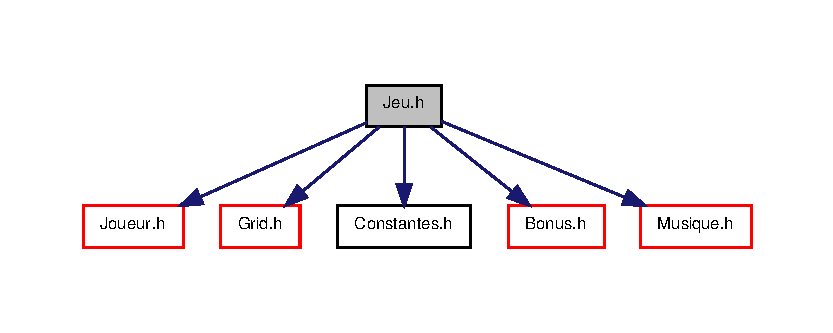
\includegraphics[width=350pt]{_jeu_8h__incl}
\end{center}
\end{figure}
Ce graphe montre quels fichiers incluent directement ou indirectement ce fichier \-:\nopagebreak
\begin{figure}[H]
\begin{center}
\leavevmode
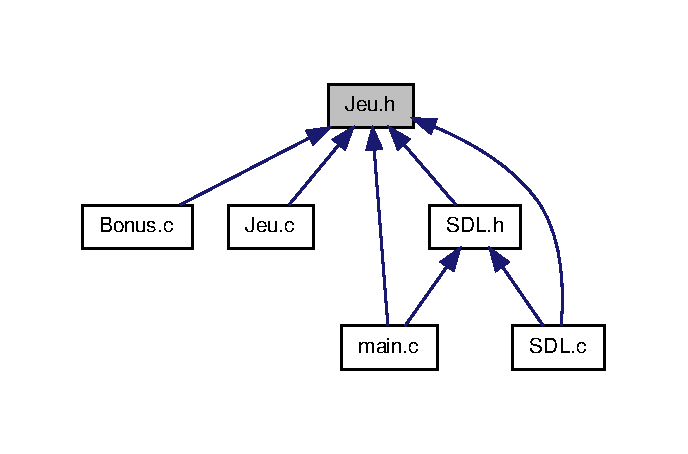
\includegraphics[width=330pt]{_jeu_8h__dep__incl}
\end{center}
\end{figure}
\subsection*{Structures de données}
\begin{DoxyCompactItemize}
\item 
struct \hyperlink{struct_jeu}{Jeu}
\end{DoxyCompactItemize}
\subsection*{Fonctions}
\begin{DoxyCompactItemize}
\item 
\hyperlink{struct_grid}{Grid} $\ast$ \hyperlink{_jeu_8h_a9cd710c657af64a74c7cc26a4e726d14}{Jeu\-Get\-Grille} (\hyperlink{struct_jeu}{Jeu} $\ast$jeu)
\item 
\hyperlink{struct_joueur}{Joueur} $\ast$ \hyperlink{_jeu_8h_a00cab8b79f7ac548749dd29b6a3dcefd}{Jeu\-Get\-Ieme\-Joueurs} (\hyperlink{struct_jeu}{Jeu} $\ast$jeu, int i)
\item 
int \hyperlink{_jeu_8h_a570c1b49959c5727b784ff980a9ca5ba}{Jeu\-Get\-Ieme\-Score} (\hyperlink{struct_jeu}{Jeu} $\ast$jeu, int i)
\item 
\hyperlink{struct_bonus}{Bonus} $\ast$ \hyperlink{_jeu_8h_a4d3ff47d4638c2a84807bc73b63c2040}{Jeu\-Get\-Ieme\-Bonus} (\hyperlink{struct_jeu}{Jeu} $\ast$jeu, int i)
\item 
int $\ast$ \hyperlink{_jeu_8h_a386693c93ff9d101058615308de79cf9}{Jeu\-Get\-Scores} (\hyperlink{struct_jeu}{Jeu} $\ast$jeu)
\item 
int \hyperlink{_jeu_8h_ae4c5515bf7a3dc1b8c55dd193559cc59}{Jeu\-Get\-Temps\-Prochain\-Bonus} (\hyperlink{struct_jeu}{Jeu} $\ast$jeu)
\item 
\hyperlink{struct_musique}{Musique} $\ast$ \hyperlink{_jeu_8h_a960195d08a333a161de438fde3f0ce9c}{Jeu\-Get\-Musique} (\hyperlink{struct_jeu}{Jeu} $\ast$jeu)
\item 
void \hyperlink{_jeu_8h_a76c474e2d5c7de3fc3f4878346c33f6d}{Jeu\-Set\-Grille} (\hyperlink{struct_jeu}{Jeu} $\ast$jeu, \hyperlink{struct_grid}{Grid} $\ast$grille)
\item 
void \hyperlink{_jeu_8h_a509c2423e3eee87b0f3ddca39e6f3fab}{Jeu\-Set\-Ieme\-Joueurs} (\hyperlink{struct_jeu}{Jeu} $\ast$jeu, \hyperlink{struct_joueur}{Joueur} $\ast$\hyperlink{struct_joueur}{Joueur}, int i)
\item 
void \hyperlink{_jeu_8h_aed59312d10d85b62fbe0320d267c1172}{Jeu\-Set\-Ieme\-Score} (\hyperlink{struct_jeu}{Jeu} $\ast$jeu, int score, int i)
\item 
void \hyperlink{_jeu_8h_acd42a024bebfff90910b9694e6958531}{Jeu\-Set\-Ieme\-Bonus} (\hyperlink{struct_jeu}{Jeu} $\ast$jeu, const \hyperlink{struct_bonus}{Bonus} $\ast$bonus, int i)
\item 
void \hyperlink{_jeu_8h_a71ff5aea9bbf81e8ecd84a2a5a0d27cb}{Jeu\-Set\-Temps\-Prochain\-Bonus} (\hyperlink{struct_jeu}{Jeu} $\ast$jeu, int temps\-Prochain\-Bonus)
\item 
void \hyperlink{_jeu_8h_a89ddb8509d691d1f24b3be6c141ee1c7}{Jeu\-Set\-Musique} (\hyperlink{struct_jeu}{Jeu} $\ast$jeu, \hyperlink{struct_musique}{Musique} $\ast$musique)
\item 
void \hyperlink{_jeu_8h_ab77436c860314786568df25bd0c2b856}{Jeu\-Constructeur} (\hyperlink{struct_jeu}{Jeu} $\ast$jeu, \hyperlink{struct_grid}{Grid} $\ast$grille, \hyperlink{struct_joueur}{Joueur} $\ast$mes\-Joueurs, int $\ast$scores, \hyperlink{struct_musique}{Musique} $\ast$musique)
\item 
void \hyperlink{_jeu_8h_a8bcba1ef69f19fb2db2610e0391cfd51}{Jeu\-Destructeur} (\hyperlink{struct_jeu}{Jeu} $\ast$jeu)
\item 
void \hyperlink{_jeu_8h_a71bdcf7116b2f14b792d222c49ff74de}{Jeu\-Evolue} (\hyperlink{struct_jeu}{Jeu} $\ast$jeu, short int $\ast$jeu\-Fini, char $\ast$nouveau\-Message, \hyperlink{_couleur_8h_aa304d0ca681f782b1d7735da33037dd7}{Couleur} $\ast$couleur\-Message)
\item 
void \hyperlink{_jeu_8h_ac2310df2f749aa58dc111b1bf906f2a8}{bouge\-Moto} (\hyperlink{struct_jeu}{Jeu} $\ast$jeu)
\item 
char \hyperlink{_jeu_8h_afc626a510d785dbffc9a7881229f0203}{test\-Collision\-Mur} (\hyperlink{struct_joueur}{Joueur} $\ast$joueur, \hyperlink{struct_grid}{Grid} $\ast$grille, char bool\-Saut)
\item 
char \hyperlink{_jeu_8h_a89c1e81df1d6a601b6683a40904d8649}{test\-Collision\-Moto} (\hyperlink{struct_moto}{Moto} $\ast$moto, \hyperlink{struct_moto}{Moto} $\ast$moto2)
\item 
void \hyperlink{_jeu_8h_a43389b43f891711881d87d46c92a53a0}{Jeu\-Action\-Clavier} (\hyperlink{struct_joueur}{Joueur} $\ast$joueur, \hyperlink{_moto_8h_a224b9163917ac32fc95a60d8c1eec3aa}{Direction} direction, \hyperlink{struct_grid}{Grid} $\ast$grille)
\item 
void \hyperlink{_jeu_8h_a4ba757faa17a6b0a476e485db82d0f54}{Jeu\-Actionne\-Bonus} (\hyperlink{struct_joueur}{Joueur} $\ast$\hyperlink{struct_joueur}{Joueur})
\item 
void \hyperlink{_jeu_8h_a5f001c65f81c3dde6d0ab2a0197558af}{Jeu\-Gere\-I\-A} (\hyperlink{struct_joueur}{Joueur} $\ast$joueur, \hyperlink{struct_jeu}{Jeu} $\ast$jeu)
\item 
void \hyperlink{_jeu_8h_aaa794bc48d4a68c8f3a3ffdb881f8eb3}{affiche\-Grille\-Analyse} (short int($\ast$grille\-Analyse)\mbox{[}\hyperlink{_constantes_8h_abf68bdf8402080e47166e730e6fa7839}{\-\_\-\-Taille\-\_\-\-Y\-\_\-\-Grille}/\hyperlink{_constantes_8h_a5486e43da0e415d8e657b6404134e6b7}{\-\_\-\-Precision\-\_\-\-Analyse\-\_\-\-I\-A}\mbox{]}\mbox{[}\hyperlink{_constantes_8h_a22ca4a20964744e6df65d2c81d5b41ff}{\-\_\-\-Taille\-\_\-\-X\-\_\-\-Grille}/\hyperlink{_constantes_8h_a5486e43da0e415d8e657b6404134e6b7}{\-\_\-\-Precision\-\_\-\-Analyse\-\_\-\-I\-A}\mbox{]})
\item 
void \hyperlink{_jeu_8h_a057ccaa58f66d1839542ce3ed73bd0d5}{affiche\-Grille\-Distances} (short int($\ast$grille\-Distance)\mbox{[}\hyperlink{_constantes_8h_abf68bdf8402080e47166e730e6fa7839}{\-\_\-\-Taille\-\_\-\-Y\-\_\-\-Grille}/\hyperlink{_constantes_8h_a5486e43da0e415d8e657b6404134e6b7}{\-\_\-\-Precision\-\_\-\-Analyse\-\_\-\-I\-A}\mbox{]}\mbox{[}\hyperlink{_constantes_8h_a22ca4a20964744e6df65d2c81d5b41ff}{\-\_\-\-Taille\-\_\-\-X\-\_\-\-Grille}/\hyperlink{_constantes_8h_a5486e43da0e415d8e657b6404134e6b7}{\-\_\-\-Precision\-\_\-\-Analyse\-\_\-\-I\-A}\mbox{]})
\item 
void \hyperlink{_jeu_8h_a3b3af5966cdc7cbf24276b5e80bdc032}{creer\-Grille\-Analyse} (short int($\ast$grille\-Analyse)\mbox{[}\hyperlink{_constantes_8h_abf68bdf8402080e47166e730e6fa7839}{\-\_\-\-Taille\-\_\-\-Y\-\_\-\-Grille}/\hyperlink{_constantes_8h_a5486e43da0e415d8e657b6404134e6b7}{\-\_\-\-Precision\-\_\-\-Analyse\-\_\-\-I\-A}\mbox{]}\mbox{[}\hyperlink{_constantes_8h_a22ca4a20964744e6df65d2c81d5b41ff}{\-\_\-\-Taille\-\_\-\-X\-\_\-\-Grille}/\hyperlink{_constantes_8h_a5486e43da0e415d8e657b6404134e6b7}{\-\_\-\-Precision\-\_\-\-Analyse\-\_\-\-I\-A}\mbox{]}, \hyperlink{struct_jeu}{Jeu} $\ast$jeu, \hyperlink{struct_joueur}{Joueur} $\ast$joueur\-I\-A)
\item 
void \hyperlink{_jeu_8h_a935de1505ff299257332d32d9b450aaa}{creer\-Grille\-Distances} (short int ligne1, short int colonne1, short int($\ast$grille\-Analyse)\mbox{[}\hyperlink{_constantes_8h_abf68bdf8402080e47166e730e6fa7839}{\-\_\-\-Taille\-\_\-\-Y\-\_\-\-Grille}/\hyperlink{_constantes_8h_a5486e43da0e415d8e657b6404134e6b7}{\-\_\-\-Precision\-\_\-\-Analyse\-\_\-\-I\-A}\mbox{]}\mbox{[}\hyperlink{_constantes_8h_a22ca4a20964744e6df65d2c81d5b41ff}{\-\_\-\-Taille\-\_\-\-X\-\_\-\-Grille}/\hyperlink{_constantes_8h_a5486e43da0e415d8e657b6404134e6b7}{\-\_\-\-Precision\-\_\-\-Analyse\-\_\-\-I\-A}\mbox{]}, short int($\ast$grille\-Distance)\mbox{[}\hyperlink{_constantes_8h_abf68bdf8402080e47166e730e6fa7839}{\-\_\-\-Taille\-\_\-\-Y\-\_\-\-Grille}/\hyperlink{_constantes_8h_a5486e43da0e415d8e657b6404134e6b7}{\-\_\-\-Precision\-\_\-\-Analyse\-\_\-\-I\-A}\mbox{]}\mbox{[}\hyperlink{_constantes_8h_a22ca4a20964744e6df65d2c81d5b41ff}{\-\_\-\-Taille\-\_\-\-X\-\_\-\-Grille}/\hyperlink{_constantes_8h_a5486e43da0e415d8e657b6404134e6b7}{\-\_\-\-Precision\-\_\-\-Analyse\-\_\-\-I\-A}\mbox{]})
\item 
short int \hyperlink{_jeu_8h_a8f806829e6634cfacfd7c54648baf3c6}{choisie\-Cible\-I\-A} (\hyperlink{struct_joueur}{Joueur} $\ast$joueur\-I\-A, \hyperlink{struct_jeu}{Jeu} $\ast$jeu, short int($\ast$grille\-Distance)\mbox{[}\hyperlink{_constantes_8h_abf68bdf8402080e47166e730e6fa7839}{\-\_\-\-Taille\-\_\-\-Y\-\_\-\-Grille}/\hyperlink{_constantes_8h_a5486e43da0e415d8e657b6404134e6b7}{\-\_\-\-Precision\-\_\-\-Analyse\-\_\-\-I\-A}\mbox{]}\mbox{[}\hyperlink{_constantes_8h_a22ca4a20964744e6df65d2c81d5b41ff}{\-\_\-\-Taille\-\_\-\-X\-\_\-\-Grille}/\hyperlink{_constantes_8h_a5486e43da0e415d8e657b6404134e6b7}{\-\_\-\-Precision\-\_\-\-Analyse\-\_\-\-I\-A}\mbox{]})
\item 
void \hyperlink{_jeu_8h_a234255b8c79dacdf45153d250a32cee5}{choisie\-Direction} (\hyperlink{struct_joueur}{Joueur} $\ast$joueur\-I\-A, \hyperlink{struct_jeu}{Jeu} $\ast$jeu, short int distance\-Joueur\-Cible, short int($\ast$grille\-Distance)\mbox{[}\hyperlink{_constantes_8h_abf68bdf8402080e47166e730e6fa7839}{\-\_\-\-Taille\-\_\-\-Y\-\_\-\-Grille}/\hyperlink{_constantes_8h_a5486e43da0e415d8e657b6404134e6b7}{\-\_\-\-Precision\-\_\-\-Analyse\-\_\-\-I\-A}\mbox{]}\mbox{[}\hyperlink{_constantes_8h_a22ca4a20964744e6df65d2c81d5b41ff}{\-\_\-\-Taille\-\_\-\-X\-\_\-\-Grille}/\hyperlink{_constantes_8h_a5486e43da0e415d8e657b6404134e6b7}{\-\_\-\-Precision\-\_\-\-Analyse\-\_\-\-I\-A}\mbox{]})
\item 
void \hyperlink{_jeu_8h_ae21534d3ce5552805c5c19c91835d45a}{indices\-Grille\-Joueur} (short int $\ast$ligne, short int $\ast$colonne, \hyperlink{struct_joueur}{Joueur} $\ast$joueur)
\item 
char \hyperlink{_jeu_8h_ac2f5807a1e5457c87bad141d69a644ad}{test\-Collision\-Generique} (float objet1\mbox{[}4\mbox{]}, float objet2\mbox{[}4\mbox{]})
\item 
char \hyperlink{_jeu_8h_a9045e76f8f81369ba40d35e5ca9b55ec}{test\-Collision\-Moto\-Bonus} (\hyperlink{struct_joueur}{Joueur} $\ast$mes\-Joueurs, \hyperlink{struct_bonus}{Bonus} $\ast$bonus)
\item 
void \hyperlink{_jeu_8h_a680716484ae925b266b97ed9cf1ca3be}{Place\-Bonus} (\hyperlink{struct_jeu}{Jeu} $\ast$jeu, \hyperlink{struct_bonus}{Bonus} $\ast$bonus)
\item 
void \hyperlink{_jeu_8h_acdb1470c32818255dca985898836aafa}{decremente\-Temps\-Bonus} (\hyperlink{struct_jeu}{Jeu} $\ast$jeu)
\item 
void \hyperlink{_jeu_8h_a9ab460d3c45562a77699da8015b3039c}{Jeu\-Test\-Regression} ()
\end{DoxyCompactItemize}


\subsection{Description détaillée}
\mbox{]} Module centrale du \hyperlink{struct_jeu}{Jeu} \begin{DoxyAuthor}{Auteur}
\{Antoine.\-C,Matthieu.\-B\} 
\end{DoxyAuthor}
\begin{DoxyVersion}{Version}
2.\-1 
\end{DoxyVersion}
\begin{DoxyDate}{Date}
13 mars 2013 
\end{DoxyDate}


Définition dans le fichier \hyperlink{_jeu_8h_source}{Jeu.\-h}.



\subsection{Documentation des fonctions}
\hypertarget{_jeu_8h_aaa794bc48d4a68c8f3a3ffdb881f8eb3}{\index{Jeu.\-h@{Jeu.\-h}!affiche\-Grille\-Analyse@{affiche\-Grille\-Analyse}}
\index{affiche\-Grille\-Analyse@{affiche\-Grille\-Analyse}!Jeu.h@{Jeu.\-h}}
\subsubsection[{affiche\-Grille\-Analyse}]{\setlength{\rightskip}{0pt plus 5cm}void affiche\-Grille\-Analyse (
\begin{DoxyParamCaption}
\item[{short int($\ast$)}]{grille\-Analyse\mbox{[}\-\_\-\-Taille\-\_\-\-Y\-\_\-\-Grille/\-\_\-\-Precision\-\_\-\-Analyse\-\_\-\-I\-A\mbox{]}\mbox{[}\-\_\-\-Taille\-\_\-\-X\-\_\-\-Grille/\-\_\-\-Precision\-\_\-\-Analyse\-\_\-\-I\-A\mbox{]}}
\end{DoxyParamCaption}
)}}\label{_jeu_8h_aaa794bc48d4a68c8f3a3ffdb881f8eb3}


Définition à la ligne 519 du fichier Jeu.\-c.

\hypertarget{_jeu_8h_a057ccaa58f66d1839542ce3ed73bd0d5}{\index{Jeu.\-h@{Jeu.\-h}!affiche\-Grille\-Distances@{affiche\-Grille\-Distances}}
\index{affiche\-Grille\-Distances@{affiche\-Grille\-Distances}!Jeu.h@{Jeu.\-h}}
\subsubsection[{affiche\-Grille\-Distances}]{\setlength{\rightskip}{0pt plus 5cm}void affiche\-Grille\-Distances (
\begin{DoxyParamCaption}
\item[{short int($\ast$)}]{grille\-Distance\mbox{[}\-\_\-\-Taille\-\_\-\-Y\-\_\-\-Grille/\-\_\-\-Precision\-\_\-\-Analyse\-\_\-\-I\-A\mbox{]}\mbox{[}\-\_\-\-Taille\-\_\-\-X\-\_\-\-Grille/\-\_\-\-Precision\-\_\-\-Analyse\-\_\-\-I\-A\mbox{]}}
\end{DoxyParamCaption}
)}}\label{_jeu_8h_a057ccaa58f66d1839542ce3ed73bd0d5}


Définition à la ligne 532 du fichier Jeu.\-c.

\hypertarget{_jeu_8h_ac2310df2f749aa58dc111b1bf906f2a8}{\index{Jeu.\-h@{Jeu.\-h}!bouge\-Moto@{bouge\-Moto}}
\index{bouge\-Moto@{bouge\-Moto}!Jeu.h@{Jeu.\-h}}
\subsubsection[{bouge\-Moto}]{\setlength{\rightskip}{0pt plus 5cm}void bouge\-Moto (
\begin{DoxyParamCaption}
\item[{{\bf Jeu} $\ast$}]{jeu}
\end{DoxyParamCaption}
)}}\label{_jeu_8h_ac2310df2f749aa58dc111b1bf906f2a8}


Définition à la ligne 234 du fichier Jeu.\-c.

\hypertarget{_jeu_8h_a8f806829e6634cfacfd7c54648baf3c6}{\index{Jeu.\-h@{Jeu.\-h}!choisie\-Cible\-I\-A@{choisie\-Cible\-I\-A}}
\index{choisie\-Cible\-I\-A@{choisie\-Cible\-I\-A}!Jeu.h@{Jeu.\-h}}
\subsubsection[{choisie\-Cible\-I\-A}]{\setlength{\rightskip}{0pt plus 5cm}short int choisie\-Cible\-I\-A (
\begin{DoxyParamCaption}
\item[{{\bf Joueur} $\ast$}]{joueur\-I\-A, }
\item[{{\bf Jeu} $\ast$}]{jeu, }
\item[{short int($\ast$)}]{grille\-Distance\mbox{[}\-\_\-\-Taille\-\_\-\-Y\-\_\-\-Grille/\-\_\-\-Precision\-\_\-\-Analyse\-\_\-\-I\-A\mbox{]}\mbox{[}\-\_\-\-Taille\-\_\-\-X\-\_\-\-Grille/\-\_\-\-Precision\-\_\-\-Analyse\-\_\-\-I\-A\mbox{]}}
\end{DoxyParamCaption}
)}}\label{_jeu_8h_a8f806829e6634cfacfd7c54648baf3c6}
!$<$On prend pour position du joueur le devant de sa moto Si cette case est inaccessible on prend une case plus loin 

Définition à la ligne 722 du fichier Jeu.\-c.

\hypertarget{_jeu_8h_a234255b8c79dacdf45153d250a32cee5}{\index{Jeu.\-h@{Jeu.\-h}!choisie\-Direction@{choisie\-Direction}}
\index{choisie\-Direction@{choisie\-Direction}!Jeu.h@{Jeu.\-h}}
\subsubsection[{choisie\-Direction}]{\setlength{\rightskip}{0pt plus 5cm}void choisie\-Direction (
\begin{DoxyParamCaption}
\item[{{\bf Joueur} $\ast$}]{joueur\-I\-A, }
\item[{{\bf Jeu} $\ast$}]{jeu, }
\item[{short int}]{distance\-Joueur\-Cible, }
\item[{short int($\ast$)}]{grille\-Distance\mbox{[}\-\_\-\-Taille\-\_\-\-Y\-\_\-\-Grille/\-\_\-\-Precision\-\_\-\-Analyse\-\_\-\-I\-A\mbox{]}\mbox{[}\-\_\-\-Taille\-\_\-\-X\-\_\-\-Grille/\-\_\-\-Precision\-\_\-\-Analyse\-\_\-\-I\-A\mbox{]}}
\end{DoxyParamCaption}
)}}\label{_jeu_8h_a234255b8c79dacdf45153d250a32cee5}
!$<$on crée 2 points pour définir la hit\-Box de la moto

!$<$Si on a pas de cible, l'I\-A essaie de survivre sans se bloquer

!$<$Amélioration possible \-: fonction aire\-Grille\-Distance qui détermine le choix de direction selon la place disponible ou même selon le mur qui va disparaitre le plus tôt

!$<$Si la position a gauche de la moto est libre,

!$<$On tourne à gauche

!$<$Si la position devant la moto est bloquée,

!$<$alors on tourne à droite

!$<$Si la position devant la moto est bloquée,

!$<$alors on tourne à droite

!$<$Si la position devant la moto est bloquée,

!$<$alors on tourne à droite

!$<$Si la position devant la moto est bloquée,

!$<$alors on tourne à droite

!$<$Si la moto va vers le bas, elle essaie de continuer à descendre,

!$<$jusqu'à ce que le bas soit bloqué

!$<$jusqu'à ce que le bas soit bloqué

!$<$Fin de l'algo de survie, ci-\/dessous l'I\-A essaie de suivre l'adversaire pour le bloquer 

Définition à la ligne 779 du fichier Jeu.\-c.

\hypertarget{_jeu_8h_a3b3af5966cdc7cbf24276b5e80bdc032}{\index{Jeu.\-h@{Jeu.\-h}!creer\-Grille\-Analyse@{creer\-Grille\-Analyse}}
\index{creer\-Grille\-Analyse@{creer\-Grille\-Analyse}!Jeu.h@{Jeu.\-h}}
\subsubsection[{creer\-Grille\-Analyse}]{\setlength{\rightskip}{0pt plus 5cm}void creer\-Grille\-Analyse (
\begin{DoxyParamCaption}
\item[{short int($\ast$)}]{grille\-Analyse\mbox{[}\-\_\-\-Taille\-\_\-\-Y\-\_\-\-Grille/\-\_\-\-Precision\-\_\-\-Analyse\-\_\-\-I\-A\mbox{]}\mbox{[}\-\_\-\-Taille\-\_\-\-X\-\_\-\-Grille/\-\_\-\-Precision\-\_\-\-Analyse\-\_\-\-I\-A\mbox{]}, }
\item[{{\bf Jeu} $\ast$}]{jeu, }
\item[{{\bf Joueur} $\ast$}]{joueur\-I\-A}
\end{DoxyParamCaption}
)}}\label{_jeu_8h_a3b3af5966cdc7cbf24276b5e80bdc032}
!$<$ On parcours les murs et on

!$<$ Crée une zone de danger autour d'eux

!$<$Si la largeur est selon x on se place au bord gauche du mur

!$<$ On crée la zone de danger au bout du mur, on décrémente le décalage

!$<$ puis on crée la zone de danger au milieu du mur etc ...

!$<$A la fin du parcours on se replace au

!$<$bord droit du mur et on recommence

!$<$Enfin on crée la zone de danger au début du mur au bord gauche puis au bord droit

!$<$Si la largeur est selon y on se place au bord haut du mur

!$<$On crée la zone de danger au bout du mur, on décrémente le décalage

!$<$puis on crée la zone de danger au milieu du mur etc ...

!$<$A la fin du parcours on se replace au

!$<$bord bas du mur et on recommence

!$<$Enfin on crée la zone de danger au début du mur au bord haut puis au bord bas 

Définition à la ligne 647 du fichier Jeu.\-c.

\hypertarget{_jeu_8h_a935de1505ff299257332d32d9b450aaa}{\index{Jeu.\-h@{Jeu.\-h}!creer\-Grille\-Distances@{creer\-Grille\-Distances}}
\index{creer\-Grille\-Distances@{creer\-Grille\-Distances}!Jeu.h@{Jeu.\-h}}
\subsubsection[{creer\-Grille\-Distances}]{\setlength{\rightskip}{0pt plus 5cm}void creer\-Grille\-Distances (
\begin{DoxyParamCaption}
\item[{short int}]{ligne1, }
\item[{short int}]{colonne1, }
\item[{short int($\ast$)}]{grille\-Analyse\mbox{[}\-\_\-\-Taille\-\_\-\-Y\-\_\-\-Grille/\-\_\-\-Precision\-\_\-\-Analyse\-\_\-\-I\-A\mbox{]}\mbox{[}\-\_\-\-Taille\-\_\-\-X\-\_\-\-Grille/\-\_\-\-Precision\-\_\-\-Analyse\-\_\-\-I\-A\mbox{]}, }
\item[{short int($\ast$)}]{grille\-Distance\mbox{[}\-\_\-\-Taille\-\_\-\-Y\-\_\-\-Grille/\-\_\-\-Precision\-\_\-\-Analyse\-\_\-\-I\-A\mbox{]}\mbox{[}\-\_\-\-Taille\-\_\-\-X\-\_\-\-Grille/\-\_\-\-Precision\-\_\-\-Analyse\-\_\-\-I\-A\mbox{]}}
\end{DoxyParamCaption}
)}}\label{_jeu_8h_a935de1505ff299257332d32d9b450aaa}


Définition à la ligne 597 du fichier Jeu.\-c.

\hypertarget{_jeu_8h_acdb1470c32818255dca985898836aafa}{\index{Jeu.\-h@{Jeu.\-h}!decremente\-Temps\-Bonus@{decremente\-Temps\-Bonus}}
\index{decremente\-Temps\-Bonus@{decremente\-Temps\-Bonus}!Jeu.h@{Jeu.\-h}}
\subsubsection[{decremente\-Temps\-Bonus}]{\setlength{\rightskip}{0pt plus 5cm}void decremente\-Temps\-Bonus (
\begin{DoxyParamCaption}
\item[{{\bf Jeu} $\ast$}]{jeu}
\end{DoxyParamCaption}
)}}\label{_jeu_8h_acdb1470c32818255dca985898836aafa}


Définition à la ligne 449 du fichier Jeu.\-c.

\hypertarget{_jeu_8h_ae21534d3ce5552805c5c19c91835d45a}{\index{Jeu.\-h@{Jeu.\-h}!indices\-Grille\-Joueur@{indices\-Grille\-Joueur}}
\index{indices\-Grille\-Joueur@{indices\-Grille\-Joueur}!Jeu.h@{Jeu.\-h}}
\subsubsection[{indices\-Grille\-Joueur}]{\setlength{\rightskip}{0pt plus 5cm}void indices\-Grille\-Joueur (
\begin{DoxyParamCaption}
\item[{short int $\ast$}]{ligne, }
\item[{short int $\ast$}]{colonne, }
\item[{{\bf Joueur} $\ast$}]{joueur}
\end{DoxyParamCaption}
)}}\label{_jeu_8h_ae21534d3ce5552805c5c19c91835d45a}


Définition à la ligne 574 du fichier Jeu.\-c.

\hypertarget{_jeu_8h_a43389b43f891711881d87d46c92a53a0}{\index{Jeu.\-h@{Jeu.\-h}!Jeu\-Action\-Clavier@{Jeu\-Action\-Clavier}}
\index{Jeu\-Action\-Clavier@{Jeu\-Action\-Clavier}!Jeu.h@{Jeu.\-h}}
\subsubsection[{Jeu\-Action\-Clavier}]{\setlength{\rightskip}{0pt plus 5cm}void Jeu\-Action\-Clavier (
\begin{DoxyParamCaption}
\item[{{\bf Joueur} $\ast$}]{joueur, }
\item[{{\bf Direction}}]{direction, }
\item[{{\bf Grid} $\ast$}]{grille}
\end{DoxyParamCaption}
)}}\label{_jeu_8h_a43389b43f891711881d87d46c92a53a0}


Définition à la ligne 159 du fichier Jeu.\-c.

\hypertarget{_jeu_8h_a4ba757faa17a6b0a476e485db82d0f54}{\index{Jeu.\-h@{Jeu.\-h}!Jeu\-Actionne\-Bonus@{Jeu\-Actionne\-Bonus}}
\index{Jeu\-Actionne\-Bonus@{Jeu\-Actionne\-Bonus}!Jeu.h@{Jeu.\-h}}
\subsubsection[{Jeu\-Actionne\-Bonus}]{\setlength{\rightskip}{0pt plus 5cm}void Jeu\-Actionne\-Bonus (
\begin{DoxyParamCaption}
\item[{{\bf Joueur} $\ast$}]{Joueur}
\end{DoxyParamCaption}
)}}\label{_jeu_8h_a4ba757faa17a6b0a476e485db82d0f54}


Définition à la ligne 470 du fichier Jeu.\-c.

\hypertarget{_jeu_8h_ab77436c860314786568df25bd0c2b856}{\index{Jeu.\-h@{Jeu.\-h}!Jeu\-Constructeur@{Jeu\-Constructeur}}
\index{Jeu\-Constructeur@{Jeu\-Constructeur}!Jeu.h@{Jeu.\-h}}
\subsubsection[{Jeu\-Constructeur}]{\setlength{\rightskip}{0pt plus 5cm}void Jeu\-Constructeur (
\begin{DoxyParamCaption}
\item[{{\bf Jeu} $\ast$}]{jeu, }
\item[{{\bf Grid} $\ast$}]{grille, }
\item[{{\bf Joueur} $\ast$}]{mes\-Joueurs, }
\item[{int $\ast$}]{scores, }
\item[{{\bf Musique} $\ast$}]{musique}
\end{DoxyParamCaption}
)}}\label{_jeu_8h_ab77436c860314786568df25bd0c2b856}


Définition à la ligne 61 du fichier Jeu.\-c.

\hypertarget{_jeu_8h_a8bcba1ef69f19fb2db2610e0391cfd51}{\index{Jeu.\-h@{Jeu.\-h}!Jeu\-Destructeur@{Jeu\-Destructeur}}
\index{Jeu\-Destructeur@{Jeu\-Destructeur}!Jeu.h@{Jeu.\-h}}
\subsubsection[{Jeu\-Destructeur}]{\setlength{\rightskip}{0pt plus 5cm}void Jeu\-Destructeur (
\begin{DoxyParamCaption}
\item[{{\bf Jeu} $\ast$}]{jeu}
\end{DoxyParamCaption}
)}}\label{_jeu_8h_a8bcba1ef69f19fb2db2610e0391cfd51}


Définition à la ligne 77 du fichier Jeu.\-c.

\hypertarget{_jeu_8h_a71bdcf7116b2f14b792d222c49ff74de}{\index{Jeu.\-h@{Jeu.\-h}!Jeu\-Evolue@{Jeu\-Evolue}}
\index{Jeu\-Evolue@{Jeu\-Evolue}!Jeu.h@{Jeu.\-h}}
\subsubsection[{Jeu\-Evolue}]{\setlength{\rightskip}{0pt plus 5cm}void Jeu\-Evolue (
\begin{DoxyParamCaption}
\item[{{\bf Jeu} $\ast$}]{jeu, }
\item[{short int $\ast$}]{jeu\-Fini, }
\item[{char $\ast$}]{nouveau\-Message, }
\item[{{\bf Couleur} $\ast$}]{couleur\-Message}
\end{DoxyParamCaption}
)}}\label{_jeu_8h_a71bdcf7116b2f14b792d222c49ff74de}


Définition à la ligne 269 du fichier Jeu.\-c.

\hypertarget{_jeu_8h_a5f001c65f81c3dde6d0ab2a0197558af}{\index{Jeu.\-h@{Jeu.\-h}!Jeu\-Gere\-I\-A@{Jeu\-Gere\-I\-A}}
\index{Jeu\-Gere\-I\-A@{Jeu\-Gere\-I\-A}!Jeu.h@{Jeu.\-h}}
\subsubsection[{Jeu\-Gere\-I\-A}]{\setlength{\rightskip}{0pt plus 5cm}void Jeu\-Gere\-I\-A (
\begin{DoxyParamCaption}
\item[{{\bf Joueur} $\ast$}]{joueur, }
\item[{{\bf Jeu} $\ast$}]{jeu}
\end{DoxyParamCaption}
)}}\label{_jeu_8h_a5f001c65f81c3dde6d0ab2a0197558af}
!$<$ On initialise la grille\-Analyse et la grille\-Distance à 0

!$<$ On initialise la position du joueur\-I\-A au devant de sa moto 

Définition à la ligne 544 du fichier Jeu.\-c.

\hypertarget{_jeu_8h_a9cd710c657af64a74c7cc26a4e726d14}{\index{Jeu.\-h@{Jeu.\-h}!Jeu\-Get\-Grille@{Jeu\-Get\-Grille}}
\index{Jeu\-Get\-Grille@{Jeu\-Get\-Grille}!Jeu.h@{Jeu.\-h}}
\subsubsection[{Jeu\-Get\-Grille}]{\setlength{\rightskip}{0pt plus 5cm}{\bf Grid}$\ast$ Jeu\-Get\-Grille (
\begin{DoxyParamCaption}
\item[{{\bf Jeu} $\ast$}]{jeu}
\end{DoxyParamCaption}
)}}\label{_jeu_8h_a9cd710c657af64a74c7cc26a4e726d14}


Définition à la ligne 20 du fichier Jeu.\-c.

\hypertarget{_jeu_8h_a4d3ff47d4638c2a84807bc73b63c2040}{\index{Jeu.\-h@{Jeu.\-h}!Jeu\-Get\-Ieme\-Bonus@{Jeu\-Get\-Ieme\-Bonus}}
\index{Jeu\-Get\-Ieme\-Bonus@{Jeu\-Get\-Ieme\-Bonus}!Jeu.h@{Jeu.\-h}}
\subsubsection[{Jeu\-Get\-Ieme\-Bonus}]{\setlength{\rightskip}{0pt plus 5cm}{\bf Bonus}$\ast$ Jeu\-Get\-Ieme\-Bonus (
\begin{DoxyParamCaption}
\item[{{\bf Jeu} $\ast$}]{jeu, }
\item[{int}]{i}
\end{DoxyParamCaption}
)}}\label{_jeu_8h_a4d3ff47d4638c2a84807bc73b63c2040}


Définition à la ligne 29 du fichier Jeu.\-c.

\hypertarget{_jeu_8h_a00cab8b79f7ac548749dd29b6a3dcefd}{\index{Jeu.\-h@{Jeu.\-h}!Jeu\-Get\-Ieme\-Joueurs@{Jeu\-Get\-Ieme\-Joueurs}}
\index{Jeu\-Get\-Ieme\-Joueurs@{Jeu\-Get\-Ieme\-Joueurs}!Jeu.h@{Jeu.\-h}}
\subsubsection[{Jeu\-Get\-Ieme\-Joueurs}]{\setlength{\rightskip}{0pt plus 5cm}{\bf Joueur}$\ast$ Jeu\-Get\-Ieme\-Joueurs (
\begin{DoxyParamCaption}
\item[{{\bf Jeu} $\ast$}]{jeu, }
\item[{int}]{i}
\end{DoxyParamCaption}
)}}\label{_jeu_8h_a00cab8b79f7ac548749dd29b6a3dcefd}


Définition à la ligne 23 du fichier Jeu.\-c.

\hypertarget{_jeu_8h_a570c1b49959c5727b784ff980a9ca5ba}{\index{Jeu.\-h@{Jeu.\-h}!Jeu\-Get\-Ieme\-Score@{Jeu\-Get\-Ieme\-Score}}
\index{Jeu\-Get\-Ieme\-Score@{Jeu\-Get\-Ieme\-Score}!Jeu.h@{Jeu.\-h}}
\subsubsection[{Jeu\-Get\-Ieme\-Score}]{\setlength{\rightskip}{0pt plus 5cm}int Jeu\-Get\-Ieme\-Score (
\begin{DoxyParamCaption}
\item[{{\bf Jeu} $\ast$}]{jeu, }
\item[{int}]{i}
\end{DoxyParamCaption}
)}}\label{_jeu_8h_a570c1b49959c5727b784ff980a9ca5ba}


Définition à la ligne 26 du fichier Jeu.\-c.

\hypertarget{_jeu_8h_a960195d08a333a161de438fde3f0ce9c}{\index{Jeu.\-h@{Jeu.\-h}!Jeu\-Get\-Musique@{Jeu\-Get\-Musique}}
\index{Jeu\-Get\-Musique@{Jeu\-Get\-Musique}!Jeu.h@{Jeu.\-h}}
\subsubsection[{Jeu\-Get\-Musique}]{\setlength{\rightskip}{0pt plus 5cm}{\bf Musique}$\ast$ Jeu\-Get\-Musique (
\begin{DoxyParamCaption}
\item[{{\bf Jeu} $\ast$}]{jeu}
\end{DoxyParamCaption}
)}}\label{_jeu_8h_a960195d08a333a161de438fde3f0ce9c}


Définition à la ligne 38 du fichier Jeu.\-c.

\hypertarget{_jeu_8h_a386693c93ff9d101058615308de79cf9}{\index{Jeu.\-h@{Jeu.\-h}!Jeu\-Get\-Scores@{Jeu\-Get\-Scores}}
\index{Jeu\-Get\-Scores@{Jeu\-Get\-Scores}!Jeu.h@{Jeu.\-h}}
\subsubsection[{Jeu\-Get\-Scores}]{\setlength{\rightskip}{0pt plus 5cm}int$\ast$ Jeu\-Get\-Scores (
\begin{DoxyParamCaption}
\item[{{\bf Jeu} $\ast$}]{jeu}
\end{DoxyParamCaption}
)}}\label{_jeu_8h_a386693c93ff9d101058615308de79cf9}


Définition à la ligne 32 du fichier Jeu.\-c.

\hypertarget{_jeu_8h_ae4c5515bf7a3dc1b8c55dd193559cc59}{\index{Jeu.\-h@{Jeu.\-h}!Jeu\-Get\-Temps\-Prochain\-Bonus@{Jeu\-Get\-Temps\-Prochain\-Bonus}}
\index{Jeu\-Get\-Temps\-Prochain\-Bonus@{Jeu\-Get\-Temps\-Prochain\-Bonus}!Jeu.h@{Jeu.\-h}}
\subsubsection[{Jeu\-Get\-Temps\-Prochain\-Bonus}]{\setlength{\rightskip}{0pt plus 5cm}int Jeu\-Get\-Temps\-Prochain\-Bonus (
\begin{DoxyParamCaption}
\item[{{\bf Jeu} $\ast$}]{jeu}
\end{DoxyParamCaption}
)}}\label{_jeu_8h_ae4c5515bf7a3dc1b8c55dd193559cc59}


Définition à la ligne 35 du fichier Jeu.\-c.

\hypertarget{_jeu_8h_a76c474e2d5c7de3fc3f4878346c33f6d}{\index{Jeu.\-h@{Jeu.\-h}!Jeu\-Set\-Grille@{Jeu\-Set\-Grille}}
\index{Jeu\-Set\-Grille@{Jeu\-Set\-Grille}!Jeu.h@{Jeu.\-h}}
\subsubsection[{Jeu\-Set\-Grille}]{\setlength{\rightskip}{0pt plus 5cm}void Jeu\-Set\-Grille (
\begin{DoxyParamCaption}
\item[{{\bf Jeu} $\ast$}]{jeu, }
\item[{{\bf Grid} $\ast$}]{grille}
\end{DoxyParamCaption}
)}}\label{_jeu_8h_a76c474e2d5c7de3fc3f4878346c33f6d}


Définition à la ligne 42 du fichier Jeu.\-c.

\hypertarget{_jeu_8h_acd42a024bebfff90910b9694e6958531}{\index{Jeu.\-h@{Jeu.\-h}!Jeu\-Set\-Ieme\-Bonus@{Jeu\-Set\-Ieme\-Bonus}}
\index{Jeu\-Set\-Ieme\-Bonus@{Jeu\-Set\-Ieme\-Bonus}!Jeu.h@{Jeu.\-h}}
\subsubsection[{Jeu\-Set\-Ieme\-Bonus}]{\setlength{\rightskip}{0pt plus 5cm}void Jeu\-Set\-Ieme\-Bonus (
\begin{DoxyParamCaption}
\item[{{\bf Jeu} $\ast$}]{jeu, }
\item[{const {\bf Bonus} $\ast$}]{bonus, }
\item[{int}]{i}
\end{DoxyParamCaption}
)}}\label{_jeu_8h_acd42a024bebfff90910b9694e6958531}


Définition à la ligne 51 du fichier Jeu.\-c.

\hypertarget{_jeu_8h_a509c2423e3eee87b0f3ddca39e6f3fab}{\index{Jeu.\-h@{Jeu.\-h}!Jeu\-Set\-Ieme\-Joueurs@{Jeu\-Set\-Ieme\-Joueurs}}
\index{Jeu\-Set\-Ieme\-Joueurs@{Jeu\-Set\-Ieme\-Joueurs}!Jeu.h@{Jeu.\-h}}
\subsubsection[{Jeu\-Set\-Ieme\-Joueurs}]{\setlength{\rightskip}{0pt plus 5cm}void Jeu\-Set\-Ieme\-Joueurs (
\begin{DoxyParamCaption}
\item[{{\bf Jeu} $\ast$}]{jeu, }
\item[{{\bf Joueur} $\ast$}]{Joueur, }
\item[{int}]{i}
\end{DoxyParamCaption}
)}}\label{_jeu_8h_a509c2423e3eee87b0f3ddca39e6f3fab}


Définition à la ligne 45 du fichier Jeu.\-c.

\hypertarget{_jeu_8h_aed59312d10d85b62fbe0320d267c1172}{\index{Jeu.\-h@{Jeu.\-h}!Jeu\-Set\-Ieme\-Score@{Jeu\-Set\-Ieme\-Score}}
\index{Jeu\-Set\-Ieme\-Score@{Jeu\-Set\-Ieme\-Score}!Jeu.h@{Jeu.\-h}}
\subsubsection[{Jeu\-Set\-Ieme\-Score}]{\setlength{\rightskip}{0pt plus 5cm}void Jeu\-Set\-Ieme\-Score (
\begin{DoxyParamCaption}
\item[{{\bf Jeu} $\ast$}]{jeu, }
\item[{int}]{score, }
\item[{int}]{i}
\end{DoxyParamCaption}
)}}\label{_jeu_8h_aed59312d10d85b62fbe0320d267c1172}


Définition à la ligne 48 du fichier Jeu.\-c.

\hypertarget{_jeu_8h_a89ddb8509d691d1f24b3be6c141ee1c7}{\index{Jeu.\-h@{Jeu.\-h}!Jeu\-Set\-Musique@{Jeu\-Set\-Musique}}
\index{Jeu\-Set\-Musique@{Jeu\-Set\-Musique}!Jeu.h@{Jeu.\-h}}
\subsubsection[{Jeu\-Set\-Musique}]{\setlength{\rightskip}{0pt plus 5cm}void Jeu\-Set\-Musique (
\begin{DoxyParamCaption}
\item[{{\bf Jeu} $\ast$}]{jeu, }
\item[{{\bf Musique} $\ast$}]{musique}
\end{DoxyParamCaption}
)}}\label{_jeu_8h_a89ddb8509d691d1f24b3be6c141ee1c7}


Définition à la ligne 57 du fichier Jeu.\-c.

\hypertarget{_jeu_8h_a71ff5aea9bbf81e8ecd84a2a5a0d27cb}{\index{Jeu.\-h@{Jeu.\-h}!Jeu\-Set\-Temps\-Prochain\-Bonus@{Jeu\-Set\-Temps\-Prochain\-Bonus}}
\index{Jeu\-Set\-Temps\-Prochain\-Bonus@{Jeu\-Set\-Temps\-Prochain\-Bonus}!Jeu.h@{Jeu.\-h}}
\subsubsection[{Jeu\-Set\-Temps\-Prochain\-Bonus}]{\setlength{\rightskip}{0pt plus 5cm}void Jeu\-Set\-Temps\-Prochain\-Bonus (
\begin{DoxyParamCaption}
\item[{{\bf Jeu} $\ast$}]{jeu, }
\item[{int}]{temps\-Prochain\-Bonus}
\end{DoxyParamCaption}
)}}\label{_jeu_8h_a71ff5aea9bbf81e8ecd84a2a5a0d27cb}


Définition à la ligne 54 du fichier Jeu.\-c.

\hypertarget{_jeu_8h_a9ab460d3c45562a77699da8015b3039c}{\index{Jeu.\-h@{Jeu.\-h}!Jeu\-Test\-Regression@{Jeu\-Test\-Regression}}
\index{Jeu\-Test\-Regression@{Jeu\-Test\-Regression}!Jeu.h@{Jeu.\-h}}
\subsubsection[{Jeu\-Test\-Regression}]{\setlength{\rightskip}{0pt plus 5cm}void Jeu\-Test\-Regression (
\begin{DoxyParamCaption}
{}
\end{DoxyParamCaption}
)}}\label{_jeu_8h_a9ab460d3c45562a77699da8015b3039c}
procédure de test 

Définition à la ligne 1089 du fichier Jeu.\-c.

\hypertarget{_jeu_8h_a680716484ae925b266b97ed9cf1ca3be}{\index{Jeu.\-h@{Jeu.\-h}!Place\-Bonus@{Place\-Bonus}}
\index{Place\-Bonus@{Place\-Bonus}!Jeu.h@{Jeu.\-h}}
\subsubsection[{Place\-Bonus}]{\setlength{\rightskip}{0pt plus 5cm}void Place\-Bonus (
\begin{DoxyParamCaption}
\item[{{\bf Jeu} $\ast$}]{jeu, }
\item[{{\bf Bonus} $\ast$}]{bonus}
\end{DoxyParamCaption}
)}}\label{_jeu_8h_a680716484ae925b266b97ed9cf1ca3be}


Définition à la ligne 503 du fichier Jeu.\-c.

\hypertarget{_jeu_8h_ac2f5807a1e5457c87bad141d69a644ad}{\index{Jeu.\-h@{Jeu.\-h}!test\-Collision\-Generique@{test\-Collision\-Generique}}
\index{test\-Collision\-Generique@{test\-Collision\-Generique}!Jeu.h@{Jeu.\-h}}
\subsubsection[{test\-Collision\-Generique}]{\setlength{\rightskip}{0pt plus 5cm}char test\-Collision\-Generique (
\begin{DoxyParamCaption}
\item[{float}]{objet1\mbox{[}4\mbox{]}, }
\item[{float}]{objet2\mbox{[}4\mbox{]}}
\end{DoxyParamCaption}
)}}\label{_jeu_8h_ac2f5807a1e5457c87bad141d69a644ad}


Définition à la ligne 88 du fichier Jeu.\-c.

\hypertarget{_jeu_8h_a89c1e81df1d6a601b6683a40904d8649}{\index{Jeu.\-h@{Jeu.\-h}!test\-Collision\-Moto@{test\-Collision\-Moto}}
\index{test\-Collision\-Moto@{test\-Collision\-Moto}!Jeu.h@{Jeu.\-h}}
\subsubsection[{test\-Collision\-Moto}]{\setlength{\rightskip}{0pt plus 5cm}char test\-Collision\-Moto (
\begin{DoxyParamCaption}
\item[{{\bf Moto} $\ast$}]{moto, }
\item[{{\bf Moto} $\ast$}]{moto2}
\end{DoxyParamCaption}
)}}\label{_jeu_8h_a89c1e81df1d6a601b6683a40904d8649}


Définition à la ligne 145 du fichier Jeu.\-c.

\hypertarget{_jeu_8h_a9045e76f8f81369ba40d35e5ca9b55ec}{\index{Jeu.\-h@{Jeu.\-h}!test\-Collision\-Moto\-Bonus@{test\-Collision\-Moto\-Bonus}}
\index{test\-Collision\-Moto\-Bonus@{test\-Collision\-Moto\-Bonus}!Jeu.h@{Jeu.\-h}}
\subsubsection[{test\-Collision\-Moto\-Bonus}]{\setlength{\rightskip}{0pt plus 5cm}char test\-Collision\-Moto\-Bonus (
\begin{DoxyParamCaption}
\item[{{\bf Joueur} $\ast$}]{mes\-Joueurs, }
\item[{{\bf Bonus} $\ast$}]{bonus}
\end{DoxyParamCaption}
)}}\label{_jeu_8h_a9045e76f8f81369ba40d35e5ca9b55ec}


Définition à la ligne 480 du fichier Jeu.\-c.

\hypertarget{_jeu_8h_afc626a510d785dbffc9a7881229f0203}{\index{Jeu.\-h@{Jeu.\-h}!test\-Collision\-Mur@{test\-Collision\-Mur}}
\index{test\-Collision\-Mur@{test\-Collision\-Mur}!Jeu.h@{Jeu.\-h}}
\subsubsection[{test\-Collision\-Mur}]{\setlength{\rightskip}{0pt plus 5cm}char test\-Collision\-Mur (
\begin{DoxyParamCaption}
\item[{{\bf Joueur} $\ast$}]{joueur, }
\item[{{\bf Grid} $\ast$}]{grille, }
\item[{char}]{bool\-Saut}
\end{DoxyParamCaption}
)}}\label{_jeu_8h_afc626a510d785dbffc9a7881229f0203}


Définition à la ligne 99 du fichier Jeu.\-c.


\hypertarget{_joueur_8c}{\section{Référence du fichier Joueur.\-c}
\label{_joueur_8c}\index{Joueur.\-c@{Joueur.\-c}}
}
{\ttfamily \#include $<$stdlib.\-h$>$}\\*
{\ttfamily \#include $<$stdio.\-h$>$}\\*
{\ttfamily \#include \char`\"{}Joueur.\-h\char`\"{}}\\*
{\ttfamily \#include \char`\"{}Moto.\-h\char`\"{}}\\*
{\ttfamily \#include \char`\"{}Controle.\-h\char`\"{}}\\*
{\ttfamily \#include \char`\"{}Couleur.\-h\char`\"{}}\\*
Graphe des dépendances par inclusion de Joueur.\-c\-:\nopagebreak
\begin{figure}[H]
\begin{center}
\leavevmode
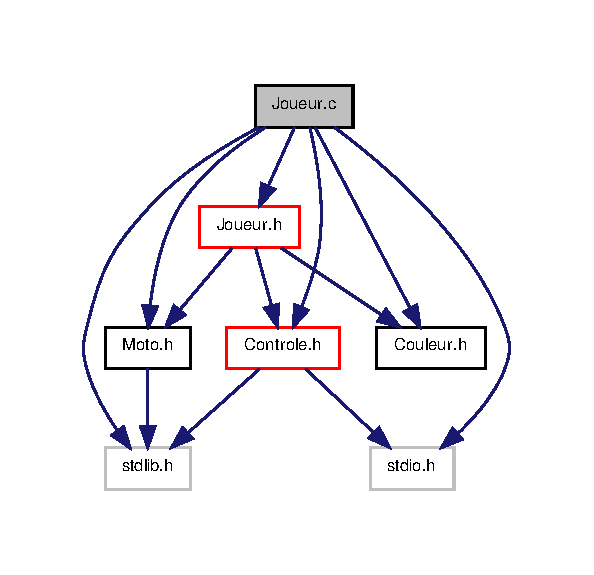
\includegraphics[width=350pt]{_joueur_8c__incl}
\end{center}
\end{figure}
\subsection*{Fonctions}
\begin{DoxyCompactItemize}
\item 
\hyperlink{struct_moto}{Moto} $\ast$ \hyperlink{_joueur_8c_a3c09cd1a406f9909b24201539e1d3d49}{Joueur\-Get\-Moto} (\hyperlink{struct_joueur}{Joueur} $\ast$joueur)
\item 
\hyperlink{struct_controle}{Controle} $\ast$ \hyperlink{_joueur_8c_afc9df65c1a7c306e987f1246a5f53b87}{Joueur\-Get\-Controle} (\hyperlink{struct_joueur}{Joueur} $\ast$joueur)
\item 
\hyperlink{_couleur_8h_aa304d0ca681f782b1d7735da33037dd7}{Couleur} \hyperlink{_joueur_8c_ab174573f7233afa24b6b2029e2427a96}{Joueur\-Get\-Couleur} (const \hyperlink{struct_joueur}{Joueur} $\ast$joueur)
\item 
\hyperlink{_joueur_8h_a43a9f41708ce5d7ddf49e05d61f48c3b}{En\-Jeu} \hyperlink{_joueur_8c_a59fc2f0e1b118c958bc22bde81fe619d}{Joueur\-Get\-En\-Jeu} (const \hyperlink{struct_joueur}{Joueur} $\ast$joueur)
\item 
\hyperlink{_effet_bonus_8h_a5c3ffd6a343fb8d5f63c87ee1a37a7fe}{Effet\-Bonus} \hyperlink{_joueur_8c_afe1d98d25a2a9915a619095e63a37d28}{Joueur\-Get\-Effet\-Bonus} (const \hyperlink{struct_joueur}{Joueur} $\ast$joueur)
\item 
short int \hyperlink{_joueur_8c_a72ad3b3bcf7dcca662d019c58f983468}{Joueur\-Get\-Numero\-Manette} (const \hyperlink{struct_joueur}{Joueur} $\ast$joueur)
\item 
int \hyperlink{_joueur_8c_a780868d4eb761d68abce085a2b040349}{Joueur\-Get\-Temps\-Bonus} (const \hyperlink{struct_joueur}{Joueur} $\ast$joueur)
\item 
\hyperlink{struct_mur}{Mur} $\ast$ \hyperlink{_joueur_8c_a9df1787fbad3851b301eb03f3e5bdf48}{Joueur\-Get\-Dernier\-Mur} (\hyperlink{struct_joueur}{Joueur} $\ast$joueur)
\item 
short int \hyperlink{_joueur_8c_a1c1f4a97676079b24229c073408d340b}{Joueur\-Get\-Booltourne} (\hyperlink{struct_joueur}{Joueur} $\ast$joueur)
\item 
short int \hyperlink{_joueur_8c_ae0849d40938feaf7a829289eb20971ab}{Joueur\-Get\-Numero\-Joueur} (\hyperlink{struct_joueur}{Joueur} $\ast$joueur)
\item 
short int \hyperlink{_joueur_8c_a0b913ee2eb6d62f1c2cf10a6bb45c828}{Joueur\-Get\-Bool\-I\-A} (\hyperlink{struct_joueur}{Joueur} $\ast$joueur)
\item 
short int \hyperlink{_joueur_8c_a7108e6f90ec1b61b4c62b55d234d6143}{Joueur\-Get\-Joueur\-Cible} (\hyperlink{struct_joueur}{Joueur} $\ast$joueur)
\item 
void \hyperlink{_joueur_8c_a1e3513e25a86b80327d96ad2fddd160c}{Joueur\-Set\-Moto} (\hyperlink{struct_joueur}{Joueur} $\ast$joueur, \hyperlink{struct_moto}{Moto} $\ast$moto)
\item 
void \hyperlink{_joueur_8c_a9af06734120dc02a68f4520e19473368}{Joueur\-Set\-Controle} (\hyperlink{struct_joueur}{Joueur} $\ast$joueur, \hyperlink{struct_controle}{Controle} $\ast$controle)
\item 
void \hyperlink{_joueur_8c_a308e870320d2641a5582bb546c6d21fc}{Joueur\-Set\-Couleur} (\hyperlink{struct_joueur}{Joueur} $\ast$joueur, \hyperlink{_couleur_8h_aa304d0ca681f782b1d7735da33037dd7}{Couleur} couleur)
\item 
void \hyperlink{_joueur_8c_a39b0f2a497b5ac7a2284513a9e19feaf}{Joueur\-Set\-En\-Jeu} (\hyperlink{struct_joueur}{Joueur} $\ast$joueur, \hyperlink{_joueur_8h_a43a9f41708ce5d7ddf49e05d61f48c3b}{En\-Jeu} en\-Jeu)
\item 
void \hyperlink{_joueur_8c_ab9b0084e52b37643b7540ef384c76f22}{Joueur\-Set\-Effet\-Bonus} (\hyperlink{struct_joueur}{Joueur} $\ast$joueur, \hyperlink{_effet_bonus_8h_a5c3ffd6a343fb8d5f63c87ee1a37a7fe}{Effet\-Bonus} effet)
\item 
void \hyperlink{_joueur_8c_a48903f3392e108482e958c7de74ea21c}{Joueur\-Set\-Numero\-Manette} (\hyperlink{struct_joueur}{Joueur} $\ast$joueur, short int numero)
\item 
void \hyperlink{_joueur_8c_a867959894ba0095f6c5d3799b8fa892f}{Joueur\-Set\-Temps\-Bonus} (\hyperlink{struct_joueur}{Joueur} $\ast$joueur, int temps\-Bonus)
\item 
void \hyperlink{_joueur_8c_adeb829f19b298f3eec06c7b13ee0c430}{Joueur\-Set\-Dernier\-Mur} (\hyperlink{struct_joueur}{Joueur} $\ast$joueur, \hyperlink{struct_mur}{Mur} $\ast$un\-Mur)
\item 
void \hyperlink{_joueur_8c_aac0438d709a0c17cf579b0f4224ebbee}{Joueur\-Set\-Booltourne} (\hyperlink{struct_joueur}{Joueur} $\ast$joueur, short int bool\-Tourne)
\item 
void \hyperlink{_joueur_8c_ab4930b1fbe66da4157c708b47d9a3f5b}{Joueur\-Set\-Numero\-Joueur} (\hyperlink{struct_joueur}{Joueur} $\ast$joueur, short int numero)
\item 
void \hyperlink{_joueur_8c_aee2c26808a926100a0497f615ece9979}{Joueur\-Set\-Bool\-I\-A} (\hyperlink{struct_joueur}{Joueur} $\ast$joueur, short int bool\-I\-A)
\item 
void \hyperlink{_joueur_8c_a9e3ee59830e0287bd639173c344ab845}{Joueur\-Set\-Joueur\-Cible} (\hyperlink{struct_joueur}{Joueur} $\ast$joueur, short int numero)
\item 
void \hyperlink{_joueur_8c_a7727f84c34d3fd32cc6f9c2ed84cf0b0}{Joueur\-Constructeur} (\hyperlink{struct_joueur}{Joueur} $\ast$joueur, \hyperlink{struct_moto}{Moto} $\ast$moto, \hyperlink{struct_controle}{Controle} $\ast$controle, \hyperlink{_couleur_8h_aa304d0ca681f782b1d7735da33037dd7}{Couleur} couleur, \hyperlink{_joueur_8h_a43a9f41708ce5d7ddf49e05d61f48c3b}{En\-Jeu} en\-Jeu, \hyperlink{_effet_bonus_8h_a5c3ffd6a343fb8d5f63c87ee1a37a7fe}{Effet\-Bonus} effet\-Actuel, short int numero\-Manette, short int numero\-Joueur, short int bool\-I\-A)
\item 
void \hyperlink{_joueur_8c_a535ea5e3fdedcdbcc7e9d84cb3b7b75e}{Joueur\-Destructeur} (\hyperlink{struct_joueur}{Joueur} $\ast$joueur)
\item 
void \hyperlink{_joueur_8c_ad628d18447d13fd4d2782e1a556c9cc3}{Joueur\-Test\-Regression} ()
\end{DoxyCompactItemize}


\subsection{Description détaillée}
\mbox{]} Module des Joueurs \begin{DoxyAuthor}{Auteur}
\{Antoine.\-C,Matthieu.\-B\} 
\end{DoxyAuthor}
\begin{DoxyVersion}{Version}
1.\-1 
\end{DoxyVersion}
\begin{DoxyDate}{Date}
19 mars 2013 
\end{DoxyDate}


Définition dans le fichier \hyperlink{_joueur_8c_source}{Joueur.\-c}.



\subsection{Documentation des fonctions}
\hypertarget{_joueur_8c_a7727f84c34d3fd32cc6f9c2ed84cf0b0}{\index{Joueur.\-c@{Joueur.\-c}!Joueur\-Constructeur@{Joueur\-Constructeur}}
\index{Joueur\-Constructeur@{Joueur\-Constructeur}!Joueur.c@{Joueur.\-c}}
\subsubsection[{Joueur\-Constructeur}]{\setlength{\rightskip}{0pt plus 5cm}void Joueur\-Constructeur (
\begin{DoxyParamCaption}
\item[{{\bf Joueur} $\ast$}]{joueur, }
\item[{{\bf Moto} $\ast$}]{moto, }
\item[{{\bf Controle} $\ast$}]{controle, }
\item[{{\bf Couleur}}]{couleur, }
\item[{{\bf En\-Jeu}}]{en\-Jeu, }
\item[{{\bf Effet\-Bonus}}]{effet\-Actuel, }
\item[{short int}]{numero\-Manette, }
\item[{short int}]{numero\-Joueur, }
\item[{short int}]{bool\-I\-A}
\end{DoxyParamCaption}
)}}\label{_joueur_8c_a7727f84c34d3fd32cc6f9c2ed84cf0b0}


Définition à la ligne 94 du fichier Joueur.\-c.

\hypertarget{_joueur_8c_a535ea5e3fdedcdbcc7e9d84cb3b7b75e}{\index{Joueur.\-c@{Joueur.\-c}!Joueur\-Destructeur@{Joueur\-Destructeur}}
\index{Joueur\-Destructeur@{Joueur\-Destructeur}!Joueur.c@{Joueur.\-c}}
\subsubsection[{Joueur\-Destructeur}]{\setlength{\rightskip}{0pt plus 5cm}void Joueur\-Destructeur (
\begin{DoxyParamCaption}
\item[{{\bf Joueur} $\ast$}]{joueur}
\end{DoxyParamCaption}
)}}\label{_joueur_8c_a535ea5e3fdedcdbcc7e9d84cb3b7b75e}


Définition à la ligne 116 du fichier Joueur.\-c.

\hypertarget{_joueur_8c_a0b913ee2eb6d62f1c2cf10a6bb45c828}{\index{Joueur.\-c@{Joueur.\-c}!Joueur\-Get\-Bool\-I\-A@{Joueur\-Get\-Bool\-I\-A}}
\index{Joueur\-Get\-Bool\-I\-A@{Joueur\-Get\-Bool\-I\-A}!Joueur.c@{Joueur.\-c}}
\subsubsection[{Joueur\-Get\-Bool\-I\-A}]{\setlength{\rightskip}{0pt plus 5cm}short int Joueur\-Get\-Bool\-I\-A (
\begin{DoxyParamCaption}
\item[{{\bf Joueur} $\ast$}]{joueur}
\end{DoxyParamCaption}
)}}\label{_joueur_8c_a0b913ee2eb6d62f1c2cf10a6bb45c828}


Définition à la ligne 47 du fichier Joueur.\-c.

\hypertarget{_joueur_8c_a1c1f4a97676079b24229c073408d340b}{\index{Joueur.\-c@{Joueur.\-c}!Joueur\-Get\-Booltourne@{Joueur\-Get\-Booltourne}}
\index{Joueur\-Get\-Booltourne@{Joueur\-Get\-Booltourne}!Joueur.c@{Joueur.\-c}}
\subsubsection[{Joueur\-Get\-Booltourne}]{\setlength{\rightskip}{0pt plus 5cm}short int Joueur\-Get\-Booltourne (
\begin{DoxyParamCaption}
\item[{{\bf Joueur} $\ast$}]{joueur}
\end{DoxyParamCaption}
)}}\label{_joueur_8c_a1c1f4a97676079b24229c073408d340b}


Définition à la ligne 41 du fichier Joueur.\-c.

\hypertarget{_joueur_8c_afc9df65c1a7c306e987f1246a5f53b87}{\index{Joueur.\-c@{Joueur.\-c}!Joueur\-Get\-Controle@{Joueur\-Get\-Controle}}
\index{Joueur\-Get\-Controle@{Joueur\-Get\-Controle}!Joueur.c@{Joueur.\-c}}
\subsubsection[{Joueur\-Get\-Controle}]{\setlength{\rightskip}{0pt plus 5cm}{\bf Controle}$\ast$ Joueur\-Get\-Controle (
\begin{DoxyParamCaption}
\item[{{\bf Joueur} $\ast$}]{joueur}
\end{DoxyParamCaption}
)}}\label{_joueur_8c_afc9df65c1a7c306e987f1246a5f53b87}


Définition à la ligne 20 du fichier Joueur.\-c.

\hypertarget{_joueur_8c_ab174573f7233afa24b6b2029e2427a96}{\index{Joueur.\-c@{Joueur.\-c}!Joueur\-Get\-Couleur@{Joueur\-Get\-Couleur}}
\index{Joueur\-Get\-Couleur@{Joueur\-Get\-Couleur}!Joueur.c@{Joueur.\-c}}
\subsubsection[{Joueur\-Get\-Couleur}]{\setlength{\rightskip}{0pt plus 5cm}{\bf Couleur} Joueur\-Get\-Couleur (
\begin{DoxyParamCaption}
\item[{const {\bf Joueur} $\ast$}]{joueur}
\end{DoxyParamCaption}
)}}\label{_joueur_8c_ab174573f7233afa24b6b2029e2427a96}


Définition à la ligne 23 du fichier Joueur.\-c.

\hypertarget{_joueur_8c_a9df1787fbad3851b301eb03f3e5bdf48}{\index{Joueur.\-c@{Joueur.\-c}!Joueur\-Get\-Dernier\-Mur@{Joueur\-Get\-Dernier\-Mur}}
\index{Joueur\-Get\-Dernier\-Mur@{Joueur\-Get\-Dernier\-Mur}!Joueur.c@{Joueur.\-c}}
\subsubsection[{Joueur\-Get\-Dernier\-Mur}]{\setlength{\rightskip}{0pt plus 5cm}{\bf Mur}$\ast$ Joueur\-Get\-Dernier\-Mur (
\begin{DoxyParamCaption}
\item[{{\bf Joueur} $\ast$}]{joueur}
\end{DoxyParamCaption}
)}}\label{_joueur_8c_a9df1787fbad3851b301eb03f3e5bdf48}


Définition à la ligne 38 du fichier Joueur.\-c.

\hypertarget{_joueur_8c_afe1d98d25a2a9915a619095e63a37d28}{\index{Joueur.\-c@{Joueur.\-c}!Joueur\-Get\-Effet\-Bonus@{Joueur\-Get\-Effet\-Bonus}}
\index{Joueur\-Get\-Effet\-Bonus@{Joueur\-Get\-Effet\-Bonus}!Joueur.c@{Joueur.\-c}}
\subsubsection[{Joueur\-Get\-Effet\-Bonus}]{\setlength{\rightskip}{0pt plus 5cm}{\bf Effet\-Bonus} Joueur\-Get\-Effet\-Bonus (
\begin{DoxyParamCaption}
\item[{const {\bf Joueur} $\ast$}]{joueur}
\end{DoxyParamCaption}
)}}\label{_joueur_8c_afe1d98d25a2a9915a619095e63a37d28}


Définition à la ligne 29 du fichier Joueur.\-c.

\hypertarget{_joueur_8c_a59fc2f0e1b118c958bc22bde81fe619d}{\index{Joueur.\-c@{Joueur.\-c}!Joueur\-Get\-En\-Jeu@{Joueur\-Get\-En\-Jeu}}
\index{Joueur\-Get\-En\-Jeu@{Joueur\-Get\-En\-Jeu}!Joueur.c@{Joueur.\-c}}
\subsubsection[{Joueur\-Get\-En\-Jeu}]{\setlength{\rightskip}{0pt plus 5cm}{\bf En\-Jeu} Joueur\-Get\-En\-Jeu (
\begin{DoxyParamCaption}
\item[{const {\bf Joueur} $\ast$}]{joueur}
\end{DoxyParamCaption}
)}}\label{_joueur_8c_a59fc2f0e1b118c958bc22bde81fe619d}


Définition à la ligne 26 du fichier Joueur.\-c.

\hypertarget{_joueur_8c_a7108e6f90ec1b61b4c62b55d234d6143}{\index{Joueur.\-c@{Joueur.\-c}!Joueur\-Get\-Joueur\-Cible@{Joueur\-Get\-Joueur\-Cible}}
\index{Joueur\-Get\-Joueur\-Cible@{Joueur\-Get\-Joueur\-Cible}!Joueur.c@{Joueur.\-c}}
\subsubsection[{Joueur\-Get\-Joueur\-Cible}]{\setlength{\rightskip}{0pt plus 5cm}short int Joueur\-Get\-Joueur\-Cible (
\begin{DoxyParamCaption}
\item[{{\bf Joueur} $\ast$}]{joueur}
\end{DoxyParamCaption}
)}}\label{_joueur_8c_a7108e6f90ec1b61b4c62b55d234d6143}


Définition à la ligne 50 du fichier Joueur.\-c.

\hypertarget{_joueur_8c_a3c09cd1a406f9909b24201539e1d3d49}{\index{Joueur.\-c@{Joueur.\-c}!Joueur\-Get\-Moto@{Joueur\-Get\-Moto}}
\index{Joueur\-Get\-Moto@{Joueur\-Get\-Moto}!Joueur.c@{Joueur.\-c}}
\subsubsection[{Joueur\-Get\-Moto}]{\setlength{\rightskip}{0pt plus 5cm}{\bf Moto}$\ast$ Joueur\-Get\-Moto (
\begin{DoxyParamCaption}
\item[{{\bf Joueur} $\ast$}]{joueur}
\end{DoxyParamCaption}
)}}\label{_joueur_8c_a3c09cd1a406f9909b24201539e1d3d49}


Définition à la ligne 17 du fichier Joueur.\-c.

\hypertarget{_joueur_8c_ae0849d40938feaf7a829289eb20971ab}{\index{Joueur.\-c@{Joueur.\-c}!Joueur\-Get\-Numero\-Joueur@{Joueur\-Get\-Numero\-Joueur}}
\index{Joueur\-Get\-Numero\-Joueur@{Joueur\-Get\-Numero\-Joueur}!Joueur.c@{Joueur.\-c}}
\subsubsection[{Joueur\-Get\-Numero\-Joueur}]{\setlength{\rightskip}{0pt plus 5cm}short int Joueur\-Get\-Numero\-Joueur (
\begin{DoxyParamCaption}
\item[{{\bf Joueur} $\ast$}]{joueur}
\end{DoxyParamCaption}
)}}\label{_joueur_8c_ae0849d40938feaf7a829289eb20971ab}


Définition à la ligne 44 du fichier Joueur.\-c.

\hypertarget{_joueur_8c_a72ad3b3bcf7dcca662d019c58f983468}{\index{Joueur.\-c@{Joueur.\-c}!Joueur\-Get\-Numero\-Manette@{Joueur\-Get\-Numero\-Manette}}
\index{Joueur\-Get\-Numero\-Manette@{Joueur\-Get\-Numero\-Manette}!Joueur.c@{Joueur.\-c}}
\subsubsection[{Joueur\-Get\-Numero\-Manette}]{\setlength{\rightskip}{0pt plus 5cm}short int Joueur\-Get\-Numero\-Manette (
\begin{DoxyParamCaption}
\item[{const {\bf Joueur} $\ast$}]{joueur}
\end{DoxyParamCaption}
)}}\label{_joueur_8c_a72ad3b3bcf7dcca662d019c58f983468}


Définition à la ligne 32 du fichier Joueur.\-c.

\hypertarget{_joueur_8c_a780868d4eb761d68abce085a2b040349}{\index{Joueur.\-c@{Joueur.\-c}!Joueur\-Get\-Temps\-Bonus@{Joueur\-Get\-Temps\-Bonus}}
\index{Joueur\-Get\-Temps\-Bonus@{Joueur\-Get\-Temps\-Bonus}!Joueur.c@{Joueur.\-c}}
\subsubsection[{Joueur\-Get\-Temps\-Bonus}]{\setlength{\rightskip}{0pt plus 5cm}int Joueur\-Get\-Temps\-Bonus (
\begin{DoxyParamCaption}
\item[{const {\bf Joueur} $\ast$}]{joueur}
\end{DoxyParamCaption}
)}}\label{_joueur_8c_a780868d4eb761d68abce085a2b040349}


Définition à la ligne 35 du fichier Joueur.\-c.

\hypertarget{_joueur_8c_aee2c26808a926100a0497f615ece9979}{\index{Joueur.\-c@{Joueur.\-c}!Joueur\-Set\-Bool\-I\-A@{Joueur\-Set\-Bool\-I\-A}}
\index{Joueur\-Set\-Bool\-I\-A@{Joueur\-Set\-Bool\-I\-A}!Joueur.c@{Joueur.\-c}}
\subsubsection[{Joueur\-Set\-Bool\-I\-A}]{\setlength{\rightskip}{0pt plus 5cm}void Joueur\-Set\-Bool\-I\-A (
\begin{DoxyParamCaption}
\item[{{\bf Joueur} $\ast$}]{joueur, }
\item[{short int}]{bool\-I\-A}
\end{DoxyParamCaption}
)}}\label{_joueur_8c_aee2c26808a926100a0497f615ece9979}


Définition à la ligne 85 du fichier Joueur.\-c.

\hypertarget{_joueur_8c_aac0438d709a0c17cf579b0f4224ebbee}{\index{Joueur.\-c@{Joueur.\-c}!Joueur\-Set\-Booltourne@{Joueur\-Set\-Booltourne}}
\index{Joueur\-Set\-Booltourne@{Joueur\-Set\-Booltourne}!Joueur.c@{Joueur.\-c}}
\subsubsection[{Joueur\-Set\-Booltourne}]{\setlength{\rightskip}{0pt plus 5cm}void Joueur\-Set\-Booltourne (
\begin{DoxyParamCaption}
\item[{{\bf Joueur} $\ast$}]{joueur, }
\item[{short int}]{bool\-Tourne}
\end{DoxyParamCaption}
)}}\label{_joueur_8c_aac0438d709a0c17cf579b0f4224ebbee}


Définition à la ligne 79 du fichier Joueur.\-c.

\hypertarget{_joueur_8c_a9af06734120dc02a68f4520e19473368}{\index{Joueur.\-c@{Joueur.\-c}!Joueur\-Set\-Controle@{Joueur\-Set\-Controle}}
\index{Joueur\-Set\-Controle@{Joueur\-Set\-Controle}!Joueur.c@{Joueur.\-c}}
\subsubsection[{Joueur\-Set\-Controle}]{\setlength{\rightskip}{0pt plus 5cm}void Joueur\-Set\-Controle (
\begin{DoxyParamCaption}
\item[{{\bf Joueur} $\ast$}]{joueur, }
\item[{{\bf Controle} $\ast$}]{controle}
\end{DoxyParamCaption}
)}}\label{_joueur_8c_a9af06734120dc02a68f4520e19473368}


Définition à la ligne 58 du fichier Joueur.\-c.

\hypertarget{_joueur_8c_a308e870320d2641a5582bb546c6d21fc}{\index{Joueur.\-c@{Joueur.\-c}!Joueur\-Set\-Couleur@{Joueur\-Set\-Couleur}}
\index{Joueur\-Set\-Couleur@{Joueur\-Set\-Couleur}!Joueur.c@{Joueur.\-c}}
\subsubsection[{Joueur\-Set\-Couleur}]{\setlength{\rightskip}{0pt plus 5cm}void Joueur\-Set\-Couleur (
\begin{DoxyParamCaption}
\item[{{\bf Joueur} $\ast$}]{joueur, }
\item[{{\bf Couleur}}]{couleur}
\end{DoxyParamCaption}
)}}\label{_joueur_8c_a308e870320d2641a5582bb546c6d21fc}


Définition à la ligne 61 du fichier Joueur.\-c.

\hypertarget{_joueur_8c_adeb829f19b298f3eec06c7b13ee0c430}{\index{Joueur.\-c@{Joueur.\-c}!Joueur\-Set\-Dernier\-Mur@{Joueur\-Set\-Dernier\-Mur}}
\index{Joueur\-Set\-Dernier\-Mur@{Joueur\-Set\-Dernier\-Mur}!Joueur.c@{Joueur.\-c}}
\subsubsection[{Joueur\-Set\-Dernier\-Mur}]{\setlength{\rightskip}{0pt plus 5cm}void Joueur\-Set\-Dernier\-Mur (
\begin{DoxyParamCaption}
\item[{{\bf Joueur} $\ast$}]{joueur, }
\item[{{\bf Mur} $\ast$}]{un\-Mur}
\end{DoxyParamCaption}
)}}\label{_joueur_8c_adeb829f19b298f3eec06c7b13ee0c430}


Définition à la ligne 76 du fichier Joueur.\-c.

\hypertarget{_joueur_8c_ab9b0084e52b37643b7540ef384c76f22}{\index{Joueur.\-c@{Joueur.\-c}!Joueur\-Set\-Effet\-Bonus@{Joueur\-Set\-Effet\-Bonus}}
\index{Joueur\-Set\-Effet\-Bonus@{Joueur\-Set\-Effet\-Bonus}!Joueur.c@{Joueur.\-c}}
\subsubsection[{Joueur\-Set\-Effet\-Bonus}]{\setlength{\rightskip}{0pt plus 5cm}void Joueur\-Set\-Effet\-Bonus (
\begin{DoxyParamCaption}
\item[{{\bf Joueur} $\ast$}]{joueur, }
\item[{{\bf Effet\-Bonus}}]{effet}
\end{DoxyParamCaption}
)}}\label{_joueur_8c_ab9b0084e52b37643b7540ef384c76f22}


Définition à la ligne 67 du fichier Joueur.\-c.

\hypertarget{_joueur_8c_a39b0f2a497b5ac7a2284513a9e19feaf}{\index{Joueur.\-c@{Joueur.\-c}!Joueur\-Set\-En\-Jeu@{Joueur\-Set\-En\-Jeu}}
\index{Joueur\-Set\-En\-Jeu@{Joueur\-Set\-En\-Jeu}!Joueur.c@{Joueur.\-c}}
\subsubsection[{Joueur\-Set\-En\-Jeu}]{\setlength{\rightskip}{0pt plus 5cm}void Joueur\-Set\-En\-Jeu (
\begin{DoxyParamCaption}
\item[{{\bf Joueur} $\ast$}]{joueur, }
\item[{{\bf En\-Jeu}}]{en\-Jeu}
\end{DoxyParamCaption}
)}}\label{_joueur_8c_a39b0f2a497b5ac7a2284513a9e19feaf}


Définition à la ligne 64 du fichier Joueur.\-c.

\hypertarget{_joueur_8c_a9e3ee59830e0287bd639173c344ab845}{\index{Joueur.\-c@{Joueur.\-c}!Joueur\-Set\-Joueur\-Cible@{Joueur\-Set\-Joueur\-Cible}}
\index{Joueur\-Set\-Joueur\-Cible@{Joueur\-Set\-Joueur\-Cible}!Joueur.c@{Joueur.\-c}}
\subsubsection[{Joueur\-Set\-Joueur\-Cible}]{\setlength{\rightskip}{0pt plus 5cm}void Joueur\-Set\-Joueur\-Cible (
\begin{DoxyParamCaption}
\item[{{\bf Joueur} $\ast$}]{joueur, }
\item[{short int}]{numero}
\end{DoxyParamCaption}
)}}\label{_joueur_8c_a9e3ee59830e0287bd639173c344ab845}


Définition à la ligne 88 du fichier Joueur.\-c.

\hypertarget{_joueur_8c_a1e3513e25a86b80327d96ad2fddd160c}{\index{Joueur.\-c@{Joueur.\-c}!Joueur\-Set\-Moto@{Joueur\-Set\-Moto}}
\index{Joueur\-Set\-Moto@{Joueur\-Set\-Moto}!Joueur.c@{Joueur.\-c}}
\subsubsection[{Joueur\-Set\-Moto}]{\setlength{\rightskip}{0pt plus 5cm}void Joueur\-Set\-Moto (
\begin{DoxyParamCaption}
\item[{{\bf Joueur} $\ast$}]{joueur, }
\item[{{\bf Moto} $\ast$}]{moto}
\end{DoxyParamCaption}
)}}\label{_joueur_8c_a1e3513e25a86b80327d96ad2fddd160c}


Définition à la ligne 55 du fichier Joueur.\-c.

\hypertarget{_joueur_8c_ab4930b1fbe66da4157c708b47d9a3f5b}{\index{Joueur.\-c@{Joueur.\-c}!Joueur\-Set\-Numero\-Joueur@{Joueur\-Set\-Numero\-Joueur}}
\index{Joueur\-Set\-Numero\-Joueur@{Joueur\-Set\-Numero\-Joueur}!Joueur.c@{Joueur.\-c}}
\subsubsection[{Joueur\-Set\-Numero\-Joueur}]{\setlength{\rightskip}{0pt plus 5cm}void Joueur\-Set\-Numero\-Joueur (
\begin{DoxyParamCaption}
\item[{{\bf Joueur} $\ast$}]{joueur, }
\item[{short int}]{numero}
\end{DoxyParamCaption}
)}}\label{_joueur_8c_ab4930b1fbe66da4157c708b47d9a3f5b}


Définition à la ligne 82 du fichier Joueur.\-c.

\hypertarget{_joueur_8c_a48903f3392e108482e958c7de74ea21c}{\index{Joueur.\-c@{Joueur.\-c}!Joueur\-Set\-Numero\-Manette@{Joueur\-Set\-Numero\-Manette}}
\index{Joueur\-Set\-Numero\-Manette@{Joueur\-Set\-Numero\-Manette}!Joueur.c@{Joueur.\-c}}
\subsubsection[{Joueur\-Set\-Numero\-Manette}]{\setlength{\rightskip}{0pt plus 5cm}void Joueur\-Set\-Numero\-Manette (
\begin{DoxyParamCaption}
\item[{{\bf Joueur} $\ast$}]{joueur, }
\item[{short int}]{numero}
\end{DoxyParamCaption}
)}}\label{_joueur_8c_a48903f3392e108482e958c7de74ea21c}


Définition à la ligne 70 du fichier Joueur.\-c.

\hypertarget{_joueur_8c_a867959894ba0095f6c5d3799b8fa892f}{\index{Joueur.\-c@{Joueur.\-c}!Joueur\-Set\-Temps\-Bonus@{Joueur\-Set\-Temps\-Bonus}}
\index{Joueur\-Set\-Temps\-Bonus@{Joueur\-Set\-Temps\-Bonus}!Joueur.c@{Joueur.\-c}}
\subsubsection[{Joueur\-Set\-Temps\-Bonus}]{\setlength{\rightskip}{0pt plus 5cm}void Joueur\-Set\-Temps\-Bonus (
\begin{DoxyParamCaption}
\item[{{\bf Joueur} $\ast$}]{joueur, }
\item[{int}]{temps\-Bonus}
\end{DoxyParamCaption}
)}}\label{_joueur_8c_a867959894ba0095f6c5d3799b8fa892f}


Définition à la ligne 73 du fichier Joueur.\-c.

\hypertarget{_joueur_8c_ad628d18447d13fd4d2782e1a556c9cc3}{\index{Joueur.\-c@{Joueur.\-c}!Joueur\-Test\-Regression@{Joueur\-Test\-Regression}}
\index{Joueur\-Test\-Regression@{Joueur\-Test\-Regression}!Joueur.c@{Joueur.\-c}}
\subsubsection[{Joueur\-Test\-Regression}]{\setlength{\rightskip}{0pt plus 5cm}Joueur\-Test\-Regression (
\begin{DoxyParamCaption}
{}
\end{DoxyParamCaption}
)}}\label{_joueur_8c_ad628d18447d13fd4d2782e1a556c9cc3}
Procedure qui teste le module \hyperlink{struct_joueur}{Joueur} 

Définition à la ligne 139 du fichier Joueur.\-c.


\hypertarget{_joueur_8h}{\section{Référence du fichier Joueur.\-h}
\label{_joueur_8h}\index{Joueur.\-h@{Joueur.\-h}}
}
{\ttfamily \#include \char`\"{}Controle.\-h\char`\"{}}\\*
{\ttfamily \#include \char`\"{}Moto.\-h\char`\"{}}\\*
{\ttfamily \#include \char`\"{}Couleur.\-h\char`\"{}}\\*
{\ttfamily \#include \char`\"{}Effet\-Bonus.\-h\char`\"{}}\\*
{\ttfamily \#include \char`\"{}Mur.\-h\char`\"{}}\\*
Graphe des dépendances par inclusion de Joueur.\-h\-:\nopagebreak
\begin{figure}[H]
\begin{center}
\leavevmode
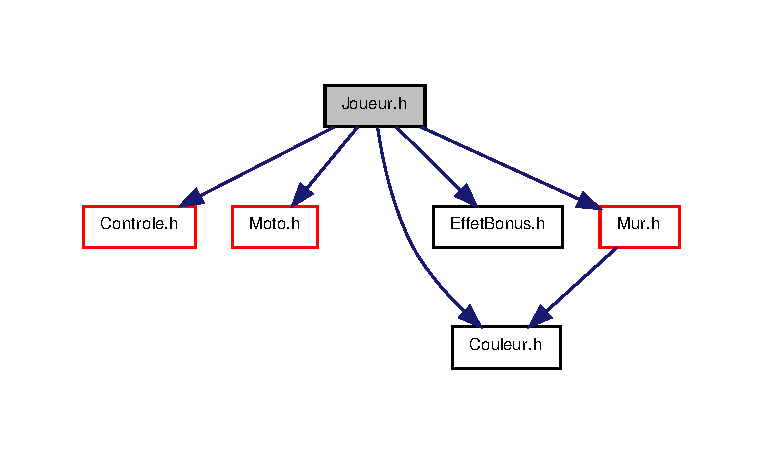
\includegraphics[width=350pt]{_joueur_8h__incl}
\end{center}
\end{figure}
Ce graphe montre quels fichiers incluent directement ou indirectement ce fichier \-:\nopagebreak
\begin{figure}[H]
\begin{center}
\leavevmode
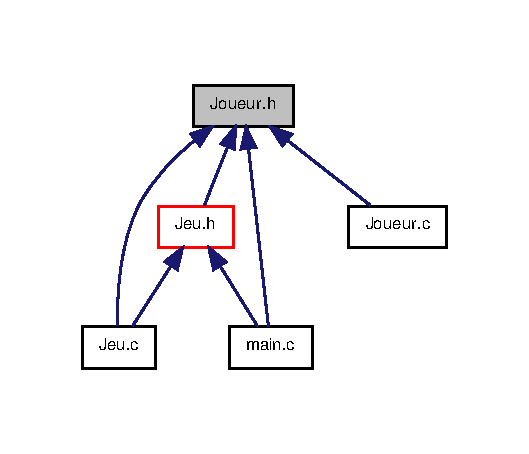
\includegraphics[width=254pt]{_joueur_8h__dep__incl}
\end{center}
\end{figure}
\subsection*{Structures de données}
\begin{DoxyCompactItemize}
\item 
struct \hyperlink{struct_joueur}{Joueur}
\end{DoxyCompactItemize}
\subsection*{Énumérations}
\begin{DoxyCompactItemize}
\item 
enum \hyperlink{_joueur_8h_a43a9f41708ce5d7ddf49e05d61f48c3b}{En\-Jeu} \{ \hyperlink{_joueur_8h_a43a9f41708ce5d7ddf49e05d61f48c3ba031fe5e154a96f85c034f6ba509060b4}{M\-O\-R\-T} =0, 
\hyperlink{_joueur_8h_a43a9f41708ce5d7ddf49e05d61f48c3ba1c63e61bcc802c01941537675433b8f4}{V\-I\-V\-A\-N\-T} =1, 
\hyperlink{_joueur_8h_a43a9f41708ce5d7ddf49e05d61f48c3ba9f2b9d7089244218315a3bbbb60bf656}{M\-O\-U\-R\-A\-N\-T} =2, 
\hyperlink{_joueur_8h_a43a9f41708ce5d7ddf49e05d61f48c3baca4e600a17ae7a7703fde47138b9eb75}{D\-O\-U\-T\-E} =3
 \}
\end{DoxyCompactItemize}
\subsection*{Fonctions}
\begin{DoxyCompactItemize}
\item 
\hyperlink{struct_moto}{Moto} $\ast$ \hyperlink{_joueur_8h_a3c09cd1a406f9909b24201539e1d3d49}{Joueur\-Get\-Moto} (\hyperlink{struct_joueur}{Joueur} $\ast$joueur)
\item 
\hyperlink{struct_controle}{Controle} $\ast$ \hyperlink{_joueur_8h_afc9df65c1a7c306e987f1246a5f53b87}{Joueur\-Get\-Controle} (\hyperlink{struct_joueur}{Joueur} $\ast$joueur)
\item 
\hyperlink{_couleur_8h_aa304d0ca681f782b1d7735da33037dd7}{Couleur} \hyperlink{_joueur_8h_ab174573f7233afa24b6b2029e2427a96}{Joueur\-Get\-Couleur} (const \hyperlink{struct_joueur}{Joueur} $\ast$joueur)
\item 
\hyperlink{_joueur_8h_a43a9f41708ce5d7ddf49e05d61f48c3b}{En\-Jeu} \hyperlink{_joueur_8h_a59fc2f0e1b118c958bc22bde81fe619d}{Joueur\-Get\-En\-Jeu} (const \hyperlink{struct_joueur}{Joueur} $\ast$joueur)
\item 
\hyperlink{_effet_bonus_8h_a5c3ffd6a343fb8d5f63c87ee1a37a7fe}{Effet\-Bonus} \hyperlink{_joueur_8h_a2bd4bb37d26013b15b02012ca325da2c}{Joueur\-Get\-Effet\-Bonus} (const \hyperlink{struct_joueur}{Joueur} $\ast$\hyperlink{struct_joueur}{Joueur})
\item 
short int \hyperlink{_joueur_8h_a72ad3b3bcf7dcca662d019c58f983468}{Joueur\-Get\-Numero\-Manette} (const \hyperlink{struct_joueur}{Joueur} $\ast$joueur)
\item 
int \hyperlink{_joueur_8h_a780868d4eb761d68abce085a2b040349}{Joueur\-Get\-Temps\-Bonus} (const \hyperlink{struct_joueur}{Joueur} $\ast$joueur)
\item 
\hyperlink{struct_mur}{Mur} $\ast$ \hyperlink{_joueur_8h_a9df1787fbad3851b301eb03f3e5bdf48}{Joueur\-Get\-Dernier\-Mur} (\hyperlink{struct_joueur}{Joueur} $\ast$joueur)
\item 
short int \hyperlink{_joueur_8h_a1c1f4a97676079b24229c073408d340b}{Joueur\-Get\-Booltourne} (\hyperlink{struct_joueur}{Joueur} $\ast$joueur)
\item 
short int \hyperlink{_joueur_8h_ae0849d40938feaf7a829289eb20971ab}{Joueur\-Get\-Numero\-Joueur} (\hyperlink{struct_joueur}{Joueur} $\ast$joueur)
\item 
short int \hyperlink{_joueur_8h_a0b913ee2eb6d62f1c2cf10a6bb45c828}{Joueur\-Get\-Bool\-I\-A} (\hyperlink{struct_joueur}{Joueur} $\ast$joueur)
\item 
short int \hyperlink{_joueur_8h_a7108e6f90ec1b61b4c62b55d234d6143}{Joueur\-Get\-Joueur\-Cible} (\hyperlink{struct_joueur}{Joueur} $\ast$joueur)
\item 
void \hyperlink{_joueur_8h_a1e3513e25a86b80327d96ad2fddd160c}{Joueur\-Set\-Moto} (\hyperlink{struct_joueur}{Joueur} $\ast$joueur, \hyperlink{struct_moto}{Moto} $\ast$moto)
\item 
void \hyperlink{_joueur_8h_a9af06734120dc02a68f4520e19473368}{Joueur\-Set\-Controle} (\hyperlink{struct_joueur}{Joueur} $\ast$joueur, \hyperlink{struct_controle}{Controle} $\ast$controle)
\item 
void \hyperlink{_joueur_8h_a308e870320d2641a5582bb546c6d21fc}{Joueur\-Set\-Couleur} (\hyperlink{struct_joueur}{Joueur} $\ast$joueur, \hyperlink{_couleur_8h_aa304d0ca681f782b1d7735da33037dd7}{Couleur} couleur)
\item 
void \hyperlink{_joueur_8h_a39b0f2a497b5ac7a2284513a9e19feaf}{Joueur\-Set\-En\-Jeu} (\hyperlink{struct_joueur}{Joueur} $\ast$joueur, \hyperlink{_joueur_8h_a43a9f41708ce5d7ddf49e05d61f48c3b}{En\-Jeu} en\-Jeu)
\item 
void \hyperlink{_joueur_8h_ab9b0084e52b37643b7540ef384c76f22}{Joueur\-Set\-Effet\-Bonus} (\hyperlink{struct_joueur}{Joueur} $\ast$joueur, \hyperlink{_effet_bonus_8h_a5c3ffd6a343fb8d5f63c87ee1a37a7fe}{Effet\-Bonus} effet)
\item 
void \hyperlink{_joueur_8h_a48903f3392e108482e958c7de74ea21c}{Joueur\-Set\-Numero\-Manette} (\hyperlink{struct_joueur}{Joueur} $\ast$joueur, short int numero)
\item 
void \hyperlink{_joueur_8h_a867959894ba0095f6c5d3799b8fa892f}{Joueur\-Set\-Temps\-Bonus} (\hyperlink{struct_joueur}{Joueur} $\ast$joueur, int temps\-Bonus)
\item 
void \hyperlink{_joueur_8h_adeb829f19b298f3eec06c7b13ee0c430}{Joueur\-Set\-Dernier\-Mur} (\hyperlink{struct_joueur}{Joueur} $\ast$joueur, \hyperlink{struct_mur}{Mur} $\ast$un\-Mur)
\item 
void \hyperlink{_joueur_8h_aac0438d709a0c17cf579b0f4224ebbee}{Joueur\-Set\-Booltourne} (\hyperlink{struct_joueur}{Joueur} $\ast$joueur, short int bool\-Tourne)
\item 
void \hyperlink{_joueur_8h_ab4930b1fbe66da4157c708b47d9a3f5b}{Joueur\-Set\-Numero\-Joueur} (\hyperlink{struct_joueur}{Joueur} $\ast$joueur, short int numero)
\item 
void \hyperlink{_joueur_8h_aee2c26808a926100a0497f615ece9979}{Joueur\-Set\-Bool\-I\-A} (\hyperlink{struct_joueur}{Joueur} $\ast$joueur, short int bool\-I\-A)
\item 
void \hyperlink{_joueur_8h_a9e3ee59830e0287bd639173c344ab845}{Joueur\-Set\-Joueur\-Cible} (\hyperlink{struct_joueur}{Joueur} $\ast$joueur, short int numero)
\item 
void \hyperlink{_joueur_8h_a7727f84c34d3fd32cc6f9c2ed84cf0b0}{Joueur\-Constructeur} (\hyperlink{struct_joueur}{Joueur} $\ast$joueur, \hyperlink{struct_moto}{Moto} $\ast$moto, \hyperlink{struct_controle}{Controle} $\ast$controle, \hyperlink{_couleur_8h_aa304d0ca681f782b1d7735da33037dd7}{Couleur} couleur, \hyperlink{_joueur_8h_a43a9f41708ce5d7ddf49e05d61f48c3b}{En\-Jeu} en\-Jeu, \hyperlink{_effet_bonus_8h_a5c3ffd6a343fb8d5f63c87ee1a37a7fe}{Effet\-Bonus} effet\-Actuel, short int numero\-Manette, short int numero\-Joueur, short int bool\-I\-A)
\item 
void \hyperlink{_joueur_8h_a535ea5e3fdedcdbcc7e9d84cb3b7b75e}{Joueur\-Destructeur} (\hyperlink{struct_joueur}{Joueur} $\ast$joueur)
\item 
void \hyperlink{_joueur_8h_aa34482db89da3f96c220e99d13465697}{Joueur\-Test\-Regression} ()
\end{DoxyCompactItemize}


\subsection{Description détaillée}
\mbox{]} Module des Joueurs \begin{DoxyAuthor}{Auteur}
\{Antoine.\-C,Matthieu.\-B\} 
\end{DoxyAuthor}
\begin{DoxyVersion}{Version}
1.\-1 
\end{DoxyVersion}
\begin{DoxyDate}{Date}
19 mars 2013 
\end{DoxyDate}


Définition dans le fichier \hyperlink{_joueur_8h_source}{Joueur.\-h}.



\subsection{Documentation du type de l'énumération}
\hypertarget{_joueur_8h_a43a9f41708ce5d7ddf49e05d61f48c3b}{\index{Joueur.\-h@{Joueur.\-h}!En\-Jeu@{En\-Jeu}}
\index{En\-Jeu@{En\-Jeu}!Joueur.h@{Joueur.\-h}}
\subsubsection[{En\-Jeu}]{\setlength{\rightskip}{0pt plus 5cm}enum {\bf En\-Jeu}}}\label{_joueur_8h_a43a9f41708ce5d7ddf49e05d61f48c3b}
\begin{Desc}
\item[Valeurs énumérées]\par
\begin{description}
\index{M\-O\-R\-T@{M\-O\-R\-T}!Joueur.\-h@{Joueur.\-h}}\index{Joueur.\-h@{Joueur.\-h}!M\-O\-R\-T@{M\-O\-R\-T}}\item[{\em 
\hypertarget{_joueur_8h_a43a9f41708ce5d7ddf49e05d61f48c3ba031fe5e154a96f85c034f6ba509060b4}{M\-O\-R\-T}\label{_joueur_8h_a43a9f41708ce5d7ddf49e05d61f48c3ba031fe5e154a96f85c034f6ba509060b4}
}]\index{V\-I\-V\-A\-N\-T@{V\-I\-V\-A\-N\-T}!Joueur.\-h@{Joueur.\-h}}\index{Joueur.\-h@{Joueur.\-h}!V\-I\-V\-A\-N\-T@{V\-I\-V\-A\-N\-T}}\item[{\em 
\hypertarget{_joueur_8h_a43a9f41708ce5d7ddf49e05d61f48c3ba1c63e61bcc802c01941537675433b8f4}{V\-I\-V\-A\-N\-T}\label{_joueur_8h_a43a9f41708ce5d7ddf49e05d61f48c3ba1c63e61bcc802c01941537675433b8f4}
}]\index{M\-O\-U\-R\-A\-N\-T@{M\-O\-U\-R\-A\-N\-T}!Joueur.\-h@{Joueur.\-h}}\index{Joueur.\-h@{Joueur.\-h}!M\-O\-U\-R\-A\-N\-T@{M\-O\-U\-R\-A\-N\-T}}\item[{\em 
\hypertarget{_joueur_8h_a43a9f41708ce5d7ddf49e05d61f48c3ba9f2b9d7089244218315a3bbbb60bf656}{M\-O\-U\-R\-A\-N\-T}\label{_joueur_8h_a43a9f41708ce5d7ddf49e05d61f48c3ba9f2b9d7089244218315a3bbbb60bf656}
}]\index{D\-O\-U\-T\-E@{D\-O\-U\-T\-E}!Joueur.\-h@{Joueur.\-h}}\index{Joueur.\-h@{Joueur.\-h}!D\-O\-U\-T\-E@{D\-O\-U\-T\-E}}\item[{\em 
\hypertarget{_joueur_8h_a43a9f41708ce5d7ddf49e05d61f48c3baca4e600a17ae7a7703fde47138b9eb75}{D\-O\-U\-T\-E}\label{_joueur_8h_a43a9f41708ce5d7ddf49e05d61f48c3baca4e600a17ae7a7703fde47138b9eb75}
}]\end{description}
\end{Desc}


Définition à la ligne 21 du fichier Joueur.\-h.



\subsection{Documentation des fonctions}
\hypertarget{_joueur_8h_a7727f84c34d3fd32cc6f9c2ed84cf0b0}{\index{Joueur.\-h@{Joueur.\-h}!Joueur\-Constructeur@{Joueur\-Constructeur}}
\index{Joueur\-Constructeur@{Joueur\-Constructeur}!Joueur.h@{Joueur.\-h}}
\subsubsection[{Joueur\-Constructeur}]{\setlength{\rightskip}{0pt plus 5cm}void Joueur\-Constructeur (
\begin{DoxyParamCaption}
\item[{{\bf Joueur} $\ast$}]{joueur, }
\item[{{\bf Moto} $\ast$}]{moto, }
\item[{{\bf Controle} $\ast$}]{controle, }
\item[{{\bf Couleur}}]{couleur, }
\item[{{\bf En\-Jeu}}]{en\-Jeu, }
\item[{{\bf Effet\-Bonus}}]{effet\-Actuel, }
\item[{short int}]{numero\-Manette, }
\item[{short int}]{numero\-Joueur, }
\item[{short int}]{bool\-I\-A}
\end{DoxyParamCaption}
)}}\label{_joueur_8h_a7727f84c34d3fd32cc6f9c2ed84cf0b0}


Définition à la ligne 94 du fichier Joueur.\-c.

\hypertarget{_joueur_8h_a535ea5e3fdedcdbcc7e9d84cb3b7b75e}{\index{Joueur.\-h@{Joueur.\-h}!Joueur\-Destructeur@{Joueur\-Destructeur}}
\index{Joueur\-Destructeur@{Joueur\-Destructeur}!Joueur.h@{Joueur.\-h}}
\subsubsection[{Joueur\-Destructeur}]{\setlength{\rightskip}{0pt plus 5cm}void Joueur\-Destructeur (
\begin{DoxyParamCaption}
\item[{{\bf Joueur} $\ast$}]{joueur}
\end{DoxyParamCaption}
)}}\label{_joueur_8h_a535ea5e3fdedcdbcc7e9d84cb3b7b75e}


Définition à la ligne 116 du fichier Joueur.\-c.

\hypertarget{_joueur_8h_a0b913ee2eb6d62f1c2cf10a6bb45c828}{\index{Joueur.\-h@{Joueur.\-h}!Joueur\-Get\-Bool\-I\-A@{Joueur\-Get\-Bool\-I\-A}}
\index{Joueur\-Get\-Bool\-I\-A@{Joueur\-Get\-Bool\-I\-A}!Joueur.h@{Joueur.\-h}}
\subsubsection[{Joueur\-Get\-Bool\-I\-A}]{\setlength{\rightskip}{0pt plus 5cm}short int Joueur\-Get\-Bool\-I\-A (
\begin{DoxyParamCaption}
\item[{{\bf Joueur} $\ast$}]{joueur}
\end{DoxyParamCaption}
)}}\label{_joueur_8h_a0b913ee2eb6d62f1c2cf10a6bb45c828}


Définition à la ligne 47 du fichier Joueur.\-c.

\hypertarget{_joueur_8h_a1c1f4a97676079b24229c073408d340b}{\index{Joueur.\-h@{Joueur.\-h}!Joueur\-Get\-Booltourne@{Joueur\-Get\-Booltourne}}
\index{Joueur\-Get\-Booltourne@{Joueur\-Get\-Booltourne}!Joueur.h@{Joueur.\-h}}
\subsubsection[{Joueur\-Get\-Booltourne}]{\setlength{\rightskip}{0pt plus 5cm}short int Joueur\-Get\-Booltourne (
\begin{DoxyParamCaption}
\item[{{\bf Joueur} $\ast$}]{joueur}
\end{DoxyParamCaption}
)}}\label{_joueur_8h_a1c1f4a97676079b24229c073408d340b}


Définition à la ligne 41 du fichier Joueur.\-c.

\hypertarget{_joueur_8h_afc9df65c1a7c306e987f1246a5f53b87}{\index{Joueur.\-h@{Joueur.\-h}!Joueur\-Get\-Controle@{Joueur\-Get\-Controle}}
\index{Joueur\-Get\-Controle@{Joueur\-Get\-Controle}!Joueur.h@{Joueur.\-h}}
\subsubsection[{Joueur\-Get\-Controle}]{\setlength{\rightskip}{0pt plus 5cm}{\bf Controle}$\ast$ Joueur\-Get\-Controle (
\begin{DoxyParamCaption}
\item[{{\bf Joueur} $\ast$}]{joueur}
\end{DoxyParamCaption}
)}}\label{_joueur_8h_afc9df65c1a7c306e987f1246a5f53b87}


Définition à la ligne 20 du fichier Joueur.\-c.

\hypertarget{_joueur_8h_ab174573f7233afa24b6b2029e2427a96}{\index{Joueur.\-h@{Joueur.\-h}!Joueur\-Get\-Couleur@{Joueur\-Get\-Couleur}}
\index{Joueur\-Get\-Couleur@{Joueur\-Get\-Couleur}!Joueur.h@{Joueur.\-h}}
\subsubsection[{Joueur\-Get\-Couleur}]{\setlength{\rightskip}{0pt plus 5cm}{\bf Couleur} Joueur\-Get\-Couleur (
\begin{DoxyParamCaption}
\item[{const {\bf Joueur} $\ast$}]{joueur}
\end{DoxyParamCaption}
)}}\label{_joueur_8h_ab174573f7233afa24b6b2029e2427a96}


Définition à la ligne 23 du fichier Joueur.\-c.

\hypertarget{_joueur_8h_a9df1787fbad3851b301eb03f3e5bdf48}{\index{Joueur.\-h@{Joueur.\-h}!Joueur\-Get\-Dernier\-Mur@{Joueur\-Get\-Dernier\-Mur}}
\index{Joueur\-Get\-Dernier\-Mur@{Joueur\-Get\-Dernier\-Mur}!Joueur.h@{Joueur.\-h}}
\subsubsection[{Joueur\-Get\-Dernier\-Mur}]{\setlength{\rightskip}{0pt plus 5cm}{\bf Mur}$\ast$ Joueur\-Get\-Dernier\-Mur (
\begin{DoxyParamCaption}
\item[{{\bf Joueur} $\ast$}]{joueur}
\end{DoxyParamCaption}
)}}\label{_joueur_8h_a9df1787fbad3851b301eb03f3e5bdf48}


Définition à la ligne 38 du fichier Joueur.\-c.

\hypertarget{_joueur_8h_a2bd4bb37d26013b15b02012ca325da2c}{\index{Joueur.\-h@{Joueur.\-h}!Joueur\-Get\-Effet\-Bonus@{Joueur\-Get\-Effet\-Bonus}}
\index{Joueur\-Get\-Effet\-Bonus@{Joueur\-Get\-Effet\-Bonus}!Joueur.h@{Joueur.\-h}}
\subsubsection[{Joueur\-Get\-Effet\-Bonus}]{\setlength{\rightskip}{0pt plus 5cm}{\bf Effet\-Bonus} Joueur\-Get\-Effet\-Bonus (
\begin{DoxyParamCaption}
\item[{const {\bf Joueur} $\ast$}]{Joueur}
\end{DoxyParamCaption}
)}}\label{_joueur_8h_a2bd4bb37d26013b15b02012ca325da2c}


Définition à la ligne 29 du fichier Joueur.\-c.

\hypertarget{_joueur_8h_a59fc2f0e1b118c958bc22bde81fe619d}{\index{Joueur.\-h@{Joueur.\-h}!Joueur\-Get\-En\-Jeu@{Joueur\-Get\-En\-Jeu}}
\index{Joueur\-Get\-En\-Jeu@{Joueur\-Get\-En\-Jeu}!Joueur.h@{Joueur.\-h}}
\subsubsection[{Joueur\-Get\-En\-Jeu}]{\setlength{\rightskip}{0pt plus 5cm}{\bf En\-Jeu} Joueur\-Get\-En\-Jeu (
\begin{DoxyParamCaption}
\item[{const {\bf Joueur} $\ast$}]{joueur}
\end{DoxyParamCaption}
)}}\label{_joueur_8h_a59fc2f0e1b118c958bc22bde81fe619d}


Définition à la ligne 26 du fichier Joueur.\-c.

\hypertarget{_joueur_8h_a7108e6f90ec1b61b4c62b55d234d6143}{\index{Joueur.\-h@{Joueur.\-h}!Joueur\-Get\-Joueur\-Cible@{Joueur\-Get\-Joueur\-Cible}}
\index{Joueur\-Get\-Joueur\-Cible@{Joueur\-Get\-Joueur\-Cible}!Joueur.h@{Joueur.\-h}}
\subsubsection[{Joueur\-Get\-Joueur\-Cible}]{\setlength{\rightskip}{0pt plus 5cm}short int Joueur\-Get\-Joueur\-Cible (
\begin{DoxyParamCaption}
\item[{{\bf Joueur} $\ast$}]{joueur}
\end{DoxyParamCaption}
)}}\label{_joueur_8h_a7108e6f90ec1b61b4c62b55d234d6143}


Définition à la ligne 50 du fichier Joueur.\-c.

\hypertarget{_joueur_8h_a3c09cd1a406f9909b24201539e1d3d49}{\index{Joueur.\-h@{Joueur.\-h}!Joueur\-Get\-Moto@{Joueur\-Get\-Moto}}
\index{Joueur\-Get\-Moto@{Joueur\-Get\-Moto}!Joueur.h@{Joueur.\-h}}
\subsubsection[{Joueur\-Get\-Moto}]{\setlength{\rightskip}{0pt plus 5cm}{\bf Moto}$\ast$ Joueur\-Get\-Moto (
\begin{DoxyParamCaption}
\item[{{\bf Joueur} $\ast$}]{joueur}
\end{DoxyParamCaption}
)}}\label{_joueur_8h_a3c09cd1a406f9909b24201539e1d3d49}


Définition à la ligne 17 du fichier Joueur.\-c.

\hypertarget{_joueur_8h_ae0849d40938feaf7a829289eb20971ab}{\index{Joueur.\-h@{Joueur.\-h}!Joueur\-Get\-Numero\-Joueur@{Joueur\-Get\-Numero\-Joueur}}
\index{Joueur\-Get\-Numero\-Joueur@{Joueur\-Get\-Numero\-Joueur}!Joueur.h@{Joueur.\-h}}
\subsubsection[{Joueur\-Get\-Numero\-Joueur}]{\setlength{\rightskip}{0pt plus 5cm}short int Joueur\-Get\-Numero\-Joueur (
\begin{DoxyParamCaption}
\item[{{\bf Joueur} $\ast$}]{joueur}
\end{DoxyParamCaption}
)}}\label{_joueur_8h_ae0849d40938feaf7a829289eb20971ab}


Définition à la ligne 44 du fichier Joueur.\-c.

\hypertarget{_joueur_8h_a72ad3b3bcf7dcca662d019c58f983468}{\index{Joueur.\-h@{Joueur.\-h}!Joueur\-Get\-Numero\-Manette@{Joueur\-Get\-Numero\-Manette}}
\index{Joueur\-Get\-Numero\-Manette@{Joueur\-Get\-Numero\-Manette}!Joueur.h@{Joueur.\-h}}
\subsubsection[{Joueur\-Get\-Numero\-Manette}]{\setlength{\rightskip}{0pt plus 5cm}short int Joueur\-Get\-Numero\-Manette (
\begin{DoxyParamCaption}
\item[{const {\bf Joueur} $\ast$}]{joueur}
\end{DoxyParamCaption}
)}}\label{_joueur_8h_a72ad3b3bcf7dcca662d019c58f983468}


Définition à la ligne 32 du fichier Joueur.\-c.

\hypertarget{_joueur_8h_a780868d4eb761d68abce085a2b040349}{\index{Joueur.\-h@{Joueur.\-h}!Joueur\-Get\-Temps\-Bonus@{Joueur\-Get\-Temps\-Bonus}}
\index{Joueur\-Get\-Temps\-Bonus@{Joueur\-Get\-Temps\-Bonus}!Joueur.h@{Joueur.\-h}}
\subsubsection[{Joueur\-Get\-Temps\-Bonus}]{\setlength{\rightskip}{0pt plus 5cm}int Joueur\-Get\-Temps\-Bonus (
\begin{DoxyParamCaption}
\item[{const {\bf Joueur} $\ast$}]{joueur}
\end{DoxyParamCaption}
)}}\label{_joueur_8h_a780868d4eb761d68abce085a2b040349}


Définition à la ligne 35 du fichier Joueur.\-c.

\hypertarget{_joueur_8h_aee2c26808a926100a0497f615ece9979}{\index{Joueur.\-h@{Joueur.\-h}!Joueur\-Set\-Bool\-I\-A@{Joueur\-Set\-Bool\-I\-A}}
\index{Joueur\-Set\-Bool\-I\-A@{Joueur\-Set\-Bool\-I\-A}!Joueur.h@{Joueur.\-h}}
\subsubsection[{Joueur\-Set\-Bool\-I\-A}]{\setlength{\rightskip}{0pt plus 5cm}void Joueur\-Set\-Bool\-I\-A (
\begin{DoxyParamCaption}
\item[{{\bf Joueur} $\ast$}]{joueur, }
\item[{short int}]{bool\-I\-A}
\end{DoxyParamCaption}
)}}\label{_joueur_8h_aee2c26808a926100a0497f615ece9979}


Définition à la ligne 85 du fichier Joueur.\-c.

\hypertarget{_joueur_8h_aac0438d709a0c17cf579b0f4224ebbee}{\index{Joueur.\-h@{Joueur.\-h}!Joueur\-Set\-Booltourne@{Joueur\-Set\-Booltourne}}
\index{Joueur\-Set\-Booltourne@{Joueur\-Set\-Booltourne}!Joueur.h@{Joueur.\-h}}
\subsubsection[{Joueur\-Set\-Booltourne}]{\setlength{\rightskip}{0pt plus 5cm}void Joueur\-Set\-Booltourne (
\begin{DoxyParamCaption}
\item[{{\bf Joueur} $\ast$}]{joueur, }
\item[{short int}]{bool\-Tourne}
\end{DoxyParamCaption}
)}}\label{_joueur_8h_aac0438d709a0c17cf579b0f4224ebbee}


Définition à la ligne 79 du fichier Joueur.\-c.

\hypertarget{_joueur_8h_a9af06734120dc02a68f4520e19473368}{\index{Joueur.\-h@{Joueur.\-h}!Joueur\-Set\-Controle@{Joueur\-Set\-Controle}}
\index{Joueur\-Set\-Controle@{Joueur\-Set\-Controle}!Joueur.h@{Joueur.\-h}}
\subsubsection[{Joueur\-Set\-Controle}]{\setlength{\rightskip}{0pt plus 5cm}void Joueur\-Set\-Controle (
\begin{DoxyParamCaption}
\item[{{\bf Joueur} $\ast$}]{joueur, }
\item[{{\bf Controle} $\ast$}]{controle}
\end{DoxyParamCaption}
)}}\label{_joueur_8h_a9af06734120dc02a68f4520e19473368}


Définition à la ligne 58 du fichier Joueur.\-c.

\hypertarget{_joueur_8h_a308e870320d2641a5582bb546c6d21fc}{\index{Joueur.\-h@{Joueur.\-h}!Joueur\-Set\-Couleur@{Joueur\-Set\-Couleur}}
\index{Joueur\-Set\-Couleur@{Joueur\-Set\-Couleur}!Joueur.h@{Joueur.\-h}}
\subsubsection[{Joueur\-Set\-Couleur}]{\setlength{\rightskip}{0pt plus 5cm}void Joueur\-Set\-Couleur (
\begin{DoxyParamCaption}
\item[{{\bf Joueur} $\ast$}]{joueur, }
\item[{{\bf Couleur}}]{couleur}
\end{DoxyParamCaption}
)}}\label{_joueur_8h_a308e870320d2641a5582bb546c6d21fc}


Définition à la ligne 61 du fichier Joueur.\-c.

\hypertarget{_joueur_8h_adeb829f19b298f3eec06c7b13ee0c430}{\index{Joueur.\-h@{Joueur.\-h}!Joueur\-Set\-Dernier\-Mur@{Joueur\-Set\-Dernier\-Mur}}
\index{Joueur\-Set\-Dernier\-Mur@{Joueur\-Set\-Dernier\-Mur}!Joueur.h@{Joueur.\-h}}
\subsubsection[{Joueur\-Set\-Dernier\-Mur}]{\setlength{\rightskip}{0pt plus 5cm}void Joueur\-Set\-Dernier\-Mur (
\begin{DoxyParamCaption}
\item[{{\bf Joueur} $\ast$}]{joueur, }
\item[{{\bf Mur} $\ast$}]{un\-Mur}
\end{DoxyParamCaption}
)}}\label{_joueur_8h_adeb829f19b298f3eec06c7b13ee0c430}


Définition à la ligne 76 du fichier Joueur.\-c.

\hypertarget{_joueur_8h_ab9b0084e52b37643b7540ef384c76f22}{\index{Joueur.\-h@{Joueur.\-h}!Joueur\-Set\-Effet\-Bonus@{Joueur\-Set\-Effet\-Bonus}}
\index{Joueur\-Set\-Effet\-Bonus@{Joueur\-Set\-Effet\-Bonus}!Joueur.h@{Joueur.\-h}}
\subsubsection[{Joueur\-Set\-Effet\-Bonus}]{\setlength{\rightskip}{0pt plus 5cm}void Joueur\-Set\-Effet\-Bonus (
\begin{DoxyParamCaption}
\item[{{\bf Joueur} $\ast$}]{joueur, }
\item[{{\bf Effet\-Bonus}}]{effet}
\end{DoxyParamCaption}
)}}\label{_joueur_8h_ab9b0084e52b37643b7540ef384c76f22}


Définition à la ligne 67 du fichier Joueur.\-c.

\hypertarget{_joueur_8h_a39b0f2a497b5ac7a2284513a9e19feaf}{\index{Joueur.\-h@{Joueur.\-h}!Joueur\-Set\-En\-Jeu@{Joueur\-Set\-En\-Jeu}}
\index{Joueur\-Set\-En\-Jeu@{Joueur\-Set\-En\-Jeu}!Joueur.h@{Joueur.\-h}}
\subsubsection[{Joueur\-Set\-En\-Jeu}]{\setlength{\rightskip}{0pt plus 5cm}void Joueur\-Set\-En\-Jeu (
\begin{DoxyParamCaption}
\item[{{\bf Joueur} $\ast$}]{joueur, }
\item[{{\bf En\-Jeu}}]{en\-Jeu}
\end{DoxyParamCaption}
)}}\label{_joueur_8h_a39b0f2a497b5ac7a2284513a9e19feaf}


Définition à la ligne 64 du fichier Joueur.\-c.

\hypertarget{_joueur_8h_a9e3ee59830e0287bd639173c344ab845}{\index{Joueur.\-h@{Joueur.\-h}!Joueur\-Set\-Joueur\-Cible@{Joueur\-Set\-Joueur\-Cible}}
\index{Joueur\-Set\-Joueur\-Cible@{Joueur\-Set\-Joueur\-Cible}!Joueur.h@{Joueur.\-h}}
\subsubsection[{Joueur\-Set\-Joueur\-Cible}]{\setlength{\rightskip}{0pt plus 5cm}void Joueur\-Set\-Joueur\-Cible (
\begin{DoxyParamCaption}
\item[{{\bf Joueur} $\ast$}]{joueur, }
\item[{short int}]{numero}
\end{DoxyParamCaption}
)}}\label{_joueur_8h_a9e3ee59830e0287bd639173c344ab845}


Définition à la ligne 88 du fichier Joueur.\-c.

\hypertarget{_joueur_8h_a1e3513e25a86b80327d96ad2fddd160c}{\index{Joueur.\-h@{Joueur.\-h}!Joueur\-Set\-Moto@{Joueur\-Set\-Moto}}
\index{Joueur\-Set\-Moto@{Joueur\-Set\-Moto}!Joueur.h@{Joueur.\-h}}
\subsubsection[{Joueur\-Set\-Moto}]{\setlength{\rightskip}{0pt plus 5cm}void Joueur\-Set\-Moto (
\begin{DoxyParamCaption}
\item[{{\bf Joueur} $\ast$}]{joueur, }
\item[{{\bf Moto} $\ast$}]{moto}
\end{DoxyParamCaption}
)}}\label{_joueur_8h_a1e3513e25a86b80327d96ad2fddd160c}


Définition à la ligne 55 du fichier Joueur.\-c.

\hypertarget{_joueur_8h_ab4930b1fbe66da4157c708b47d9a3f5b}{\index{Joueur.\-h@{Joueur.\-h}!Joueur\-Set\-Numero\-Joueur@{Joueur\-Set\-Numero\-Joueur}}
\index{Joueur\-Set\-Numero\-Joueur@{Joueur\-Set\-Numero\-Joueur}!Joueur.h@{Joueur.\-h}}
\subsubsection[{Joueur\-Set\-Numero\-Joueur}]{\setlength{\rightskip}{0pt plus 5cm}void Joueur\-Set\-Numero\-Joueur (
\begin{DoxyParamCaption}
\item[{{\bf Joueur} $\ast$}]{joueur, }
\item[{short int}]{numero}
\end{DoxyParamCaption}
)}}\label{_joueur_8h_ab4930b1fbe66da4157c708b47d9a3f5b}


Définition à la ligne 82 du fichier Joueur.\-c.

\hypertarget{_joueur_8h_a48903f3392e108482e958c7de74ea21c}{\index{Joueur.\-h@{Joueur.\-h}!Joueur\-Set\-Numero\-Manette@{Joueur\-Set\-Numero\-Manette}}
\index{Joueur\-Set\-Numero\-Manette@{Joueur\-Set\-Numero\-Manette}!Joueur.h@{Joueur.\-h}}
\subsubsection[{Joueur\-Set\-Numero\-Manette}]{\setlength{\rightskip}{0pt plus 5cm}void Joueur\-Set\-Numero\-Manette (
\begin{DoxyParamCaption}
\item[{{\bf Joueur} $\ast$}]{joueur, }
\item[{short int}]{numero}
\end{DoxyParamCaption}
)}}\label{_joueur_8h_a48903f3392e108482e958c7de74ea21c}


Définition à la ligne 70 du fichier Joueur.\-c.

\hypertarget{_joueur_8h_a867959894ba0095f6c5d3799b8fa892f}{\index{Joueur.\-h@{Joueur.\-h}!Joueur\-Set\-Temps\-Bonus@{Joueur\-Set\-Temps\-Bonus}}
\index{Joueur\-Set\-Temps\-Bonus@{Joueur\-Set\-Temps\-Bonus}!Joueur.h@{Joueur.\-h}}
\subsubsection[{Joueur\-Set\-Temps\-Bonus}]{\setlength{\rightskip}{0pt plus 5cm}void Joueur\-Set\-Temps\-Bonus (
\begin{DoxyParamCaption}
\item[{{\bf Joueur} $\ast$}]{joueur, }
\item[{int}]{temps\-Bonus}
\end{DoxyParamCaption}
)}}\label{_joueur_8h_a867959894ba0095f6c5d3799b8fa892f}


Définition à la ligne 73 du fichier Joueur.\-c.

\hypertarget{_joueur_8h_aa34482db89da3f96c220e99d13465697}{\index{Joueur.\-h@{Joueur.\-h}!Joueur\-Test\-Regression@{Joueur\-Test\-Regression}}
\index{Joueur\-Test\-Regression@{Joueur\-Test\-Regression}!Joueur.h@{Joueur.\-h}}
\subsubsection[{Joueur\-Test\-Regression}]{\setlength{\rightskip}{0pt plus 5cm}void Joueur\-Test\-Regression (
\begin{DoxyParamCaption}
{}
\end{DoxyParamCaption}
)}}\label{_joueur_8h_aa34482db89da3f96c220e99d13465697}
Procedure qui teste le module \hyperlink{struct_joueur}{Joueur} 

Définition à la ligne 139 du fichier Joueur.\-c.


\hypertarget{_joystick_8c}{\section{Référence du fichier Joystick.\-c}
\label{_joystick_8c}\index{Joystick.\-c@{Joystick.\-c}}
}
{\ttfamily \#include $<$stdlib.\-h$>$}\\*
{\ttfamily \#include $<$S\-D\-L/\-S\-D\-L.\-h$>$}\\*
{\ttfamily \#include \char`\"{}Joystick.\-h\char`\"{}}\\*
Graphe des dépendances par inclusion de Joystick.\-c\-:\nopagebreak
\begin{figure}[H]
\begin{center}
\leavevmode
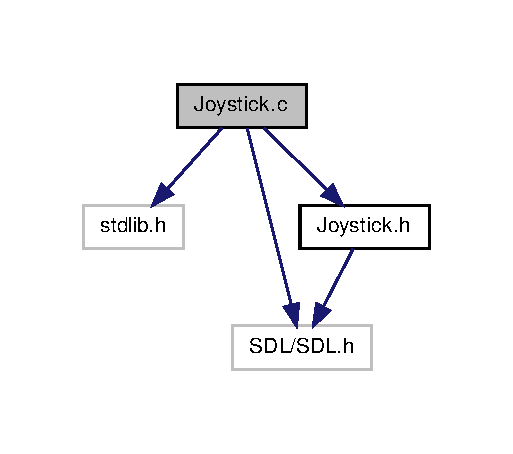
\includegraphics[width=226pt]{_joystick_8c__incl}
\end{center}
\end{figure}
\subsection*{Fonctions}
\begin{DoxyCompactItemize}
\item 
void \hyperlink{_joystick_8c_ad146b7d348cac88b34f110a94d7be261}{initialiser\-Manette} (\hyperlink{struct_manette}{Manette} $\ast$manette, int numero\-Joystick)
\item 
void \hyperlink{_joystick_8c_a5b653de255c8eba83785537e28183913}{detruire\-Manette} (\hyperlink{struct_manette}{Manette} $\ast$manette)
\item 
void \hyperlink{_joystick_8c_a7ca1494e4a16b50fefc58546440e4c1f}{update\-Event} (\hyperlink{struct_manette}{Manette} $\ast$manette, S\-D\-L\-\_\-\-Event evenements)
\item 
void \hyperlink{_joystick_8c_a127d271e79132d7a6c331f22524018e7}{Joystick\-Test\-Regression} ()
\end{DoxyCompactItemize}


\subsection{Description détaillée}
\mbox{]} Module des manettes \begin{DoxyAuthor}{Auteur}
\{Antoine.\-C,Matthieu.\-B\} 
\end{DoxyAuthor}
\begin{DoxyVersion}{Version}
0.\-1 
\end{DoxyVersion}
\begin{DoxyDate}{Date}
11 avril 2013 
\end{DoxyDate}


Définition dans le fichier \hyperlink{_joystick_8c_source}{Joystick.\-c}.



\subsection{Documentation des fonctions}
\hypertarget{_joystick_8c_a5b653de255c8eba83785537e28183913}{\index{Joystick.\-c@{Joystick.\-c}!detruire\-Manette@{detruire\-Manette}}
\index{detruire\-Manette@{detruire\-Manette}!Joystick.c@{Joystick.\-c}}
\subsubsection[{detruire\-Manette}]{\setlength{\rightskip}{0pt plus 5cm}void detruire\-Manette (
\begin{DoxyParamCaption}
\item[{{\bf Manette} $\ast$}]{manette}
\end{DoxyParamCaption}
)}}\label{_joystick_8c_a5b653de255c8eba83785537e28183913}


Définition à la ligne 46 du fichier Joystick.\-c.

\hypertarget{_joystick_8c_ad146b7d348cac88b34f110a94d7be261}{\index{Joystick.\-c@{Joystick.\-c}!initialiser\-Manette@{initialiser\-Manette}}
\index{initialiser\-Manette@{initialiser\-Manette}!Joystick.c@{Joystick.\-c}}
\subsubsection[{initialiser\-Manette}]{\setlength{\rightskip}{0pt plus 5cm}void initialiser\-Manette (
\begin{DoxyParamCaption}
\item[{{\bf Manette} $\ast$}]{manette, }
\item[{int}]{numero\-Joystick}
\end{DoxyParamCaption}
)}}\label{_joystick_8c_ad146b7d348cac88b34f110a94d7be261}


Définition à la ligne 14 du fichier Joystick.\-c.

\hypertarget{_joystick_8c_a127d271e79132d7a6c331f22524018e7}{\index{Joystick.\-c@{Joystick.\-c}!Joystick\-Test\-Regression@{Joystick\-Test\-Regression}}
\index{Joystick\-Test\-Regression@{Joystick\-Test\-Regression}!Joystick.c@{Joystick.\-c}}
\subsubsection[{Joystick\-Test\-Regression}]{\setlength{\rightskip}{0pt plus 5cm}Joystick\-Test\-Regression (
\begin{DoxyParamCaption}
{}
\end{DoxyParamCaption}
)}}\label{_joystick_8c_a127d271e79132d7a6c331f22524018e7}
fonction qui teste le module 

Définition à la ligne 91 du fichier Joystick.\-c.

\hypertarget{_joystick_8c_a7ca1494e4a16b50fefc58546440e4c1f}{\index{Joystick.\-c@{Joystick.\-c}!update\-Event@{update\-Event}}
\index{update\-Event@{update\-Event}!Joystick.c@{Joystick.\-c}}
\subsubsection[{update\-Event}]{\setlength{\rightskip}{0pt plus 5cm}void update\-Event (
\begin{DoxyParamCaption}
\item[{{\bf Manette} $\ast$}]{manette, }
\item[{S\-D\-L\-\_\-\-Event}]{evenements}
\end{DoxyParamCaption}
)}}\label{_joystick_8c_a7ca1494e4a16b50fefc58546440e4c1f}


Définition à la ligne 59 du fichier Joystick.\-c.


\hypertarget{_joystick_8h}{\section{Référence du fichier Joystick.\-h}
\label{_joystick_8h}\index{Joystick.\-h@{Joystick.\-h}}
}
{\ttfamily \#include $<$S\-D\-L/\-S\-D\-L.\-h$>$}\\*
Graphe des dépendances par inclusion de Joystick.\-h\-:\nopagebreak
\begin{figure}[H]
\begin{center}
\leavevmode
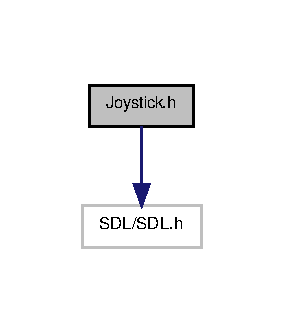
\includegraphics[width=146pt]{_joystick_8h__incl}
\end{center}
\end{figure}
Ce graphe montre quels fichiers incluent directement ou indirectement ce fichier \-:\nopagebreak
\begin{figure}[H]
\begin{center}
\leavevmode
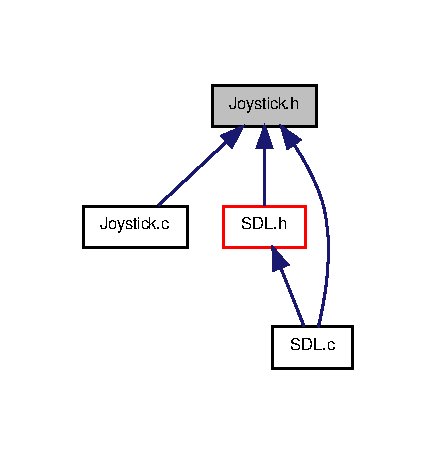
\includegraphics[width=254pt]{_joystick_8h__dep__incl}
\end{center}
\end{figure}
\subsection*{Structures de données}
\begin{DoxyCompactItemize}
\item 
struct \hyperlink{struct_manette}{Manette}
\end{DoxyCompactItemize}
\subsection*{Fonctions}
\begin{DoxyCompactItemize}
\item 
void \hyperlink{_joystick_8h_ad146b7d348cac88b34f110a94d7be261}{initialiser\-Manette} (\hyperlink{struct_manette}{Manette} $\ast$manette, int numero\-Joystick)
\item 
void \hyperlink{_joystick_8h_a5b653de255c8eba83785537e28183913}{detruire\-Manette} (\hyperlink{struct_manette}{Manette} $\ast$manette)
\item 
void \hyperlink{_joystick_8h_a40eeef47716755bc5966509b894a0c37}{update\-Event} (\hyperlink{struct_manette}{Manette} $\ast$manette, S\-D\-L\-\_\-\-Event evenement)
\item 
void \hyperlink{_joystick_8h_a8cae93745b6ebe7fc4c3e7374583b037}{Joystick\-Test\-Regression} ()
\end{DoxyCompactItemize}


\subsection{Description détaillée}
\mbox{]} Module des manettes \begin{DoxyAuthor}{Auteur}
\{Antoine.\-C,Matthieu.\-B\} 
\end{DoxyAuthor}
\begin{DoxyVersion}{Version}
0.\-1 
\end{DoxyVersion}
\begin{DoxyDate}{Date}
11 avril 2013 
\end{DoxyDate}


Définition dans le fichier \hyperlink{_joystick_8h_source}{Joystick.\-h}.



\subsection{Documentation des fonctions}
\hypertarget{_joystick_8h_a5b653de255c8eba83785537e28183913}{\index{Joystick.\-h@{Joystick.\-h}!detruire\-Manette@{detruire\-Manette}}
\index{detruire\-Manette@{detruire\-Manette}!Joystick.h@{Joystick.\-h}}
\subsubsection[{detruire\-Manette}]{\setlength{\rightskip}{0pt plus 5cm}void detruire\-Manette (
\begin{DoxyParamCaption}
\item[{{\bf Manette} $\ast$}]{manette}
\end{DoxyParamCaption}
)}}\label{_joystick_8h_a5b653de255c8eba83785537e28183913}


Définition à la ligne 46 du fichier Joystick.\-c.

\hypertarget{_joystick_8h_ad146b7d348cac88b34f110a94d7be261}{\index{Joystick.\-h@{Joystick.\-h}!initialiser\-Manette@{initialiser\-Manette}}
\index{initialiser\-Manette@{initialiser\-Manette}!Joystick.h@{Joystick.\-h}}
\subsubsection[{initialiser\-Manette}]{\setlength{\rightskip}{0pt plus 5cm}void initialiser\-Manette (
\begin{DoxyParamCaption}
\item[{{\bf Manette} $\ast$}]{manette, }
\item[{int}]{numero\-Joystick}
\end{DoxyParamCaption}
)}}\label{_joystick_8h_ad146b7d348cac88b34f110a94d7be261}


Définition à la ligne 14 du fichier Joystick.\-c.

\hypertarget{_joystick_8h_a8cae93745b6ebe7fc4c3e7374583b037}{\index{Joystick.\-h@{Joystick.\-h}!Joystick\-Test\-Regression@{Joystick\-Test\-Regression}}
\index{Joystick\-Test\-Regression@{Joystick\-Test\-Regression}!Joystick.h@{Joystick.\-h}}
\subsubsection[{Joystick\-Test\-Regression}]{\setlength{\rightskip}{0pt plus 5cm}void Joystick\-Test\-Regression (
\begin{DoxyParamCaption}
{}
\end{DoxyParamCaption}
)}}\label{_joystick_8h_a8cae93745b6ebe7fc4c3e7374583b037}
fonction qui teste le module 

Définition à la ligne 91 du fichier Joystick.\-c.

\hypertarget{_joystick_8h_a40eeef47716755bc5966509b894a0c37}{\index{Joystick.\-h@{Joystick.\-h}!update\-Event@{update\-Event}}
\index{update\-Event@{update\-Event}!Joystick.h@{Joystick.\-h}}
\subsubsection[{update\-Event}]{\setlength{\rightskip}{0pt plus 5cm}void update\-Event (
\begin{DoxyParamCaption}
\item[{{\bf Manette} $\ast$}]{manette, }
\item[{S\-D\-L\-\_\-\-Event}]{evenement}
\end{DoxyParamCaption}
)}}\label{_joystick_8h_a40eeef47716755bc5966509b894a0c37}


Définition à la ligne 59 du fichier Joystick.\-c.


\hypertarget{main_8c}{\section{Référence du fichier main.\-c}
\label{main_8c}\index{main.\-c@{main.\-c}}
}


\hyperlink{main_8c}{main.\-c}  


{\ttfamily \#include $<$stdlib.\-h$>$}\\*
{\ttfamily \#include $<$stdio.\-h$>$}\\*
{\ttfamily \#include $<$assert.\-h$>$}\\*
{\ttfamily \#include \char`\"{}Mur.\-h\char`\"{}}\\*
{\ttfamily \#include \char`\"{}Moto.\-h\char`\"{}}\\*
{\ttfamily \#include \char`\"{}Controle.\-h\char`\"{}}\\*
{\ttfamily \#include \char`\"{}Joueur.\-h\char`\"{}}\\*
{\ttfamily \#include \char`\"{}Grid.\-h\char`\"{}}\\*
{\ttfamily \#include \char`\"{}Jeu.\-h\char`\"{}}\\*
{\ttfamily \#include \char`\"{}S\-D\-L.\-h\char`\"{}}\\*
{\ttfamily \#include \char`\"{}Bonus.\-h\char`\"{}}\\*
{\ttfamily \#include \char`\"{}Constantes.\-h\char`\"{}}\\*
{\ttfamily \#include \char`\"{}Musique.\-h\char`\"{}}\\*
{\ttfamily \#include $<$time.\-h$>$}\\*
Graphe des dépendances par inclusion de main.\-c\-:
\nopagebreak
\begin{figure}[H]
\begin{center}
\leavevmode
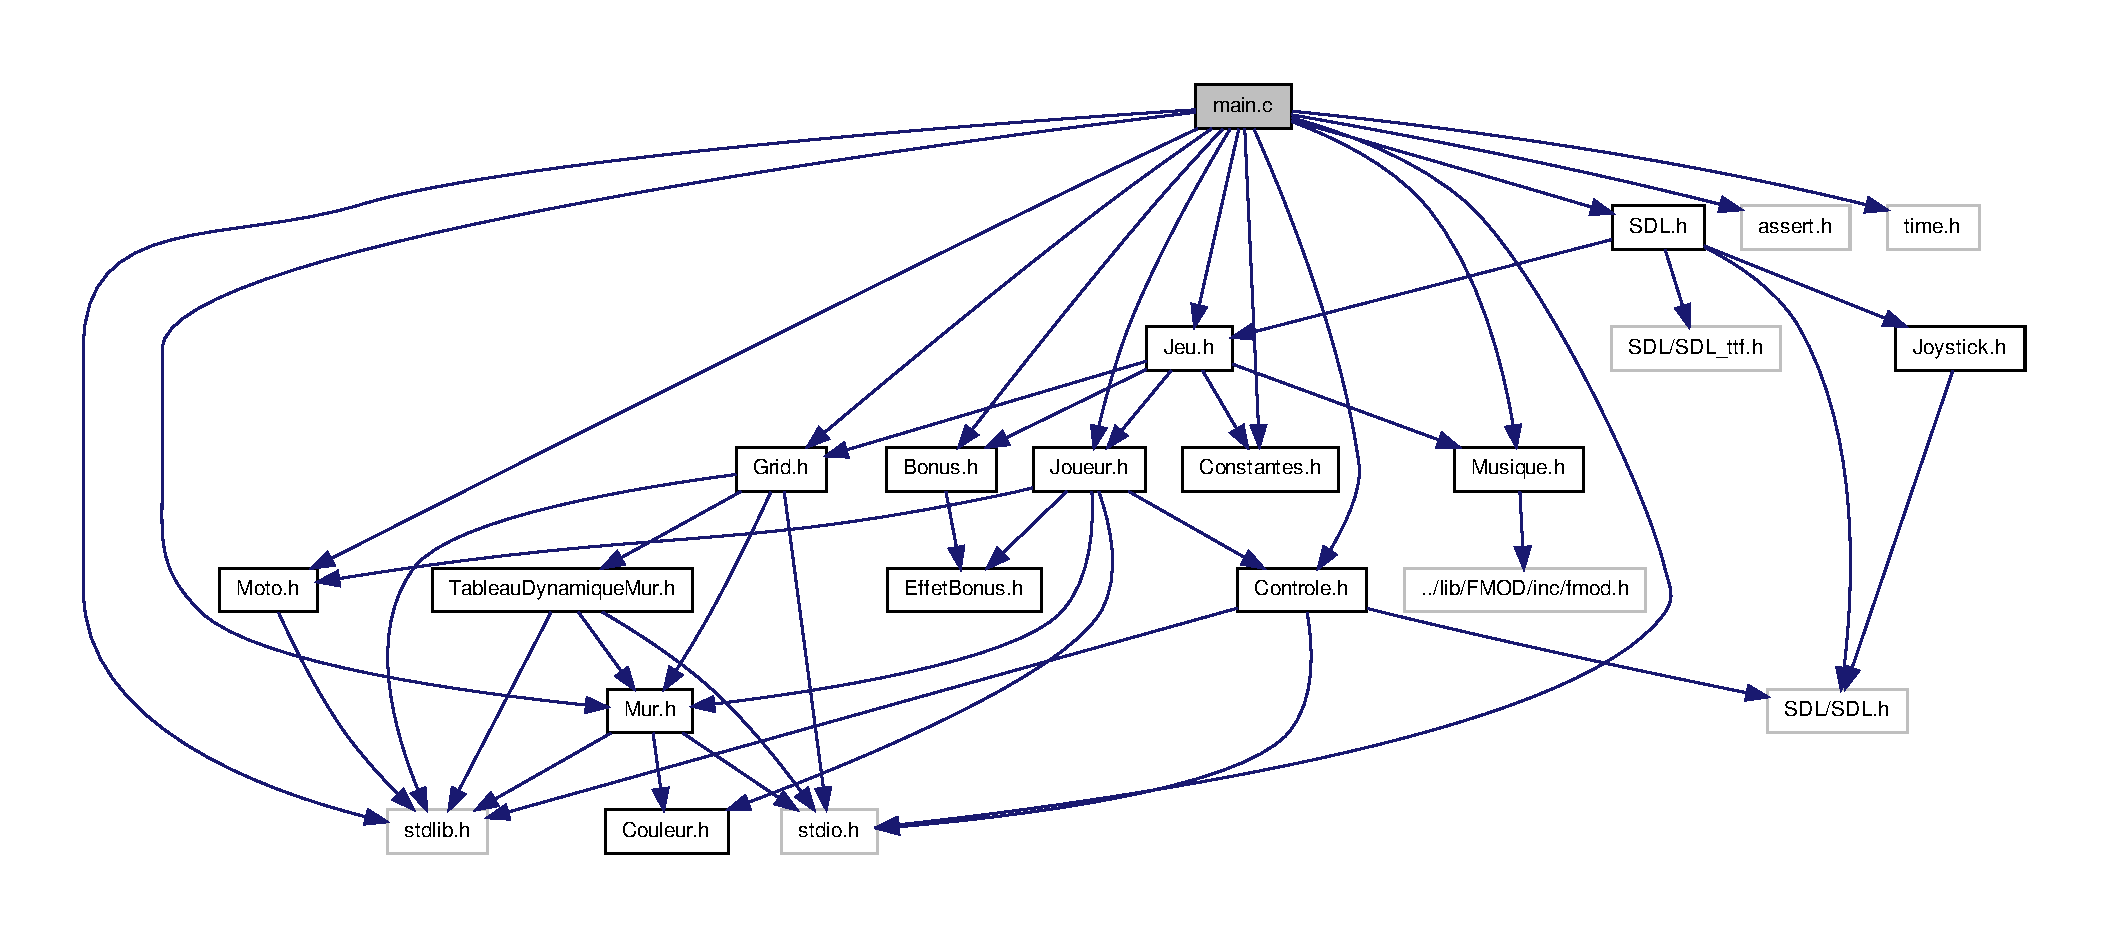
\includegraphics[width=350pt]{main_8c__incl}
\end{center}
\end{figure}
\subsection*{Fonctions}
\begin{DoxyCompactItemize}
\item 
int \hyperlink{main_8c_ae66f6b31b5ad750f1fe042a706a4e3d4}{main} ()
\end{DoxyCompactItemize}


\subsection{Description détaillée}
\hyperlink{main_8c}{main.\-c} \mbox{]} \begin{DoxyAuthor}{Auteur}
\{Antoine.\-C,Matthieu.\-B\} 
\end{DoxyAuthor}
\begin{DoxyVersion}{Version}
1.\-0 
\end{DoxyVersion}
\begin{DoxyDate}{Date}
13 mars 2013 
\end{DoxyDate}


Définition dans le fichier \hyperlink{main_8c_source}{main.\-c}.



\subsection{Documentation des fonctions}
\hypertarget{main_8c_ae66f6b31b5ad750f1fe042a706a4e3d4}{\index{main.\-c@{main.\-c}!main@{main}}
\index{main@{main}!main.c@{main.\-c}}
\subsubsection[{main}]{\setlength{\rightskip}{0pt plus 5cm}int main (
\begin{DoxyParamCaption}
{}
\end{DoxyParamCaption}
)}}\label{main_8c_ae66f6b31b5ad750f1fe042a706a4e3d4}


Définition à la ligne 24 du fichier main.\-c.


\hypertarget{_moto_8c}{\section{Référence du fichier Moto.\-c}
\label{_moto_8c}\index{Moto.\-c@{Moto.\-c}}
}
{\ttfamily \#include $<$stdlib.\-h$>$}\\*
{\ttfamily \#include $<$stdio.\-h$>$}\\*
{\ttfamily \#include \char`\"{}Moto.\-h\char`\"{}}\\*
Graphe des dépendances par inclusion de Moto.\-c\-:\nopagebreak
\begin{figure}[H]
\begin{center}
\leavevmode
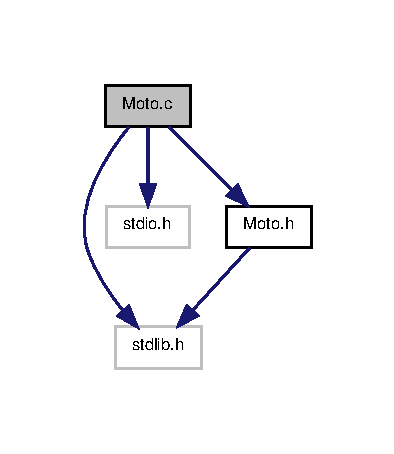
\includegraphics[width=189pt]{_moto_8c__incl}
\end{center}
\end{figure}
\subsection*{Fonctions}
\begin{DoxyCompactItemize}
\item 
float \hyperlink{_moto_8c_a4156c04a753d20234c7882f960830e72}{Moto\-Get\-Position\-X} (const \hyperlink{struct_moto}{Moto} $\ast$moto)
\item 
float \hyperlink{_moto_8c_a62ff0acafab13335eb75daddd0f1b842}{Moto\-Get\-Position\-Y} (const \hyperlink{struct_moto}{Moto} $\ast$moto)
\item 
unsigned int \hyperlink{_moto_8c_a3c4edf672fcff5483b3805ea4850b0bf}{Moto\-Get\-Taille\-X} (const \hyperlink{struct_moto}{Moto} $\ast$moto)
\item 
unsigned int \hyperlink{_moto_8c_aa2e2c249d5453b97bbe5a0a3dcfec6c0}{Moto\-Get\-Taille\-Y} (const \hyperlink{struct_moto}{Moto} $\ast$moto)
\item 
float \hyperlink{_moto_8c_a211ad1ea110f768b154253e64386c999}{Moto\-Get\-Vitesse} (const \hyperlink{struct_moto}{Moto} $\ast$moto)
\item 
\hyperlink{_moto_8h_a224b9163917ac32fc95a60d8c1eec3aa}{Direction} \hyperlink{_moto_8c_a3b507a0e47b0c30898ff385292ad44ba}{Moto\-Get\-Direction} (const \hyperlink{struct_moto}{Moto} $\ast$moto)
\item 
void \hyperlink{_moto_8c_afc3d835e1a44c42e70b20288c4094696}{Moto\-Set\-Position\-X} (\hyperlink{struct_moto}{Moto} $\ast$moto, float pos\-X)
\item 
void \hyperlink{_moto_8c_a933ac221bf445ac7ba78ec4d68718c11}{Moto\-Set\-Position\-Y} (\hyperlink{struct_moto}{Moto} $\ast$moto, float pos\-Y)
\item 
void \hyperlink{_moto_8c_adf496889057950aa5b2c9d61e83870ff}{Moto\-Set\-Taille\-X} (\hyperlink{struct_moto}{Moto} $\ast$moto, unsigned int taille\-X)
\item 
void \hyperlink{_moto_8c_aa457e0e893057e65dd374802bc3144cd}{Moto\-Set\-Taille\-Y} (\hyperlink{struct_moto}{Moto} $\ast$moto, unsigned int taille\-Y)
\item 
void \hyperlink{_moto_8c_ab62e1b43e1a546b1552db8dde7a692b6}{Moto\-Set\-Vitesse} (\hyperlink{struct_moto}{Moto} $\ast$moto, float vitesse)
\item 
void \hyperlink{_moto_8c_a5e01d8daba6d2035d6a54f28a193ce35}{Moto\-Set\-Direction} (\hyperlink{struct_moto}{Moto} $\ast$moto, \hyperlink{_moto_8h_a224b9163917ac32fc95a60d8c1eec3aa}{Direction} direction)
\item 
void \hyperlink{_moto_8c_adaa34f67eeb029811b895f62c48e1e37}{Moto\-Constructeur} (\hyperlink{struct_moto}{Moto} $\ast$moto, float pos\-X, float pos\-Y, unsigned int taille\-X, unsigned int taille\-Y, float vitesse, \hyperlink{_moto_8h_a224b9163917ac32fc95a60d8c1eec3aa}{Direction} direction)
\item 
void \hyperlink{_moto_8c_a8c1f41e71c00d38b29d1b8ab0e93d542}{Moto\-Destructeur} (\hyperlink{struct_moto}{Moto} $\ast$moto)
\item 
void \hyperlink{_moto_8c_aee18c911ddc26580170985f506538dcb}{Moto\-Test\-Regression} ()
\end{DoxyCompactItemize}


\subsection{Description détaillée}
\mbox{]} Module des Motos du jeu \begin{DoxyAuthor}{Auteur}
\{Antoine.\-C,Matthieu.\-B\} 
\end{DoxyAuthor}
\begin{DoxyVersion}{Version}
0.\-1 
\end{DoxyVersion}
\begin{DoxyDate}{Date}
13 mars 2013 
\end{DoxyDate}


Définition dans le fichier \hyperlink{_moto_8c_source}{Moto.\-c}.



\subsection{Documentation des fonctions}
\hypertarget{_moto_8c_adaa34f67eeb029811b895f62c48e1e37}{\index{Moto.\-c@{Moto.\-c}!Moto\-Constructeur@{Moto\-Constructeur}}
\index{Moto\-Constructeur@{Moto\-Constructeur}!Moto.c@{Moto.\-c}}
\subsubsection[{Moto\-Constructeur}]{\setlength{\rightskip}{0pt plus 5cm}void Moto\-Constructeur (
\begin{DoxyParamCaption}
\item[{{\bf Moto} $\ast$}]{moto, }
\item[{float}]{pos\-X, }
\item[{float}]{pos\-Y, }
\item[{unsigned int}]{taille\-X, }
\item[{unsigned int}]{taille\-Y, }
\item[{float}]{vitesse, }
\item[{{\bf Direction}}]{direction}
\end{DoxyParamCaption}
)}}\label{_moto_8c_adaa34f67eeb029811b895f62c48e1e37}


Définition à la ligne 51 du fichier Moto.\-c.

\hypertarget{_moto_8c_a8c1f41e71c00d38b29d1b8ab0e93d542}{\index{Moto.\-c@{Moto.\-c}!Moto\-Destructeur@{Moto\-Destructeur}}
\index{Moto\-Destructeur@{Moto\-Destructeur}!Moto.c@{Moto.\-c}}
\subsubsection[{Moto\-Destructeur}]{\setlength{\rightskip}{0pt plus 5cm}void Moto\-Destructeur (
\begin{DoxyParamCaption}
\item[{{\bf Moto} $\ast$}]{moto}
\end{DoxyParamCaption}
)}}\label{_moto_8c_a8c1f41e71c00d38b29d1b8ab0e93d542}


Définition à la ligne 59 du fichier Moto.\-c.

\hypertarget{_moto_8c_a3b507a0e47b0c30898ff385292ad44ba}{\index{Moto.\-c@{Moto.\-c}!Moto\-Get\-Direction@{Moto\-Get\-Direction}}
\index{Moto\-Get\-Direction@{Moto\-Get\-Direction}!Moto.c@{Moto.\-c}}
\subsubsection[{Moto\-Get\-Direction}]{\setlength{\rightskip}{0pt plus 5cm}{\bf Direction} Moto\-Get\-Direction (
\begin{DoxyParamCaption}
\item[{const {\bf Moto} $\ast$}]{moto}
\end{DoxyParamCaption}
)}}\label{_moto_8c_a3b507a0e47b0c30898ff385292ad44ba}


Définition à la ligne 28 du fichier Moto.\-c.

\hypertarget{_moto_8c_a4156c04a753d20234c7882f960830e72}{\index{Moto.\-c@{Moto.\-c}!Moto\-Get\-Position\-X@{Moto\-Get\-Position\-X}}
\index{Moto\-Get\-Position\-X@{Moto\-Get\-Position\-X}!Moto.c@{Moto.\-c}}
\subsubsection[{Moto\-Get\-Position\-X}]{\setlength{\rightskip}{0pt plus 5cm}float Moto\-Get\-Position\-X (
\begin{DoxyParamCaption}
\item[{const {\bf Moto} $\ast$}]{moto}
\end{DoxyParamCaption}
)}}\label{_moto_8c_a4156c04a753d20234c7882f960830e72}


Définition à la ligne 13 du fichier Moto.\-c.

\hypertarget{_moto_8c_a62ff0acafab13335eb75daddd0f1b842}{\index{Moto.\-c@{Moto.\-c}!Moto\-Get\-Position\-Y@{Moto\-Get\-Position\-Y}}
\index{Moto\-Get\-Position\-Y@{Moto\-Get\-Position\-Y}!Moto.c@{Moto.\-c}}
\subsubsection[{Moto\-Get\-Position\-Y}]{\setlength{\rightskip}{0pt plus 5cm}float Moto\-Get\-Position\-Y (
\begin{DoxyParamCaption}
\item[{const {\bf Moto} $\ast$}]{moto}
\end{DoxyParamCaption}
)}}\label{_moto_8c_a62ff0acafab13335eb75daddd0f1b842}


Définition à la ligne 16 du fichier Moto.\-c.

\hypertarget{_moto_8c_a3c4edf672fcff5483b3805ea4850b0bf}{\index{Moto.\-c@{Moto.\-c}!Moto\-Get\-Taille\-X@{Moto\-Get\-Taille\-X}}
\index{Moto\-Get\-Taille\-X@{Moto\-Get\-Taille\-X}!Moto.c@{Moto.\-c}}
\subsubsection[{Moto\-Get\-Taille\-X}]{\setlength{\rightskip}{0pt plus 5cm}unsigned int Moto\-Get\-Taille\-X (
\begin{DoxyParamCaption}
\item[{const {\bf Moto} $\ast$}]{moto}
\end{DoxyParamCaption}
)}}\label{_moto_8c_a3c4edf672fcff5483b3805ea4850b0bf}


Définition à la ligne 19 du fichier Moto.\-c.

\hypertarget{_moto_8c_aa2e2c249d5453b97bbe5a0a3dcfec6c0}{\index{Moto.\-c@{Moto.\-c}!Moto\-Get\-Taille\-Y@{Moto\-Get\-Taille\-Y}}
\index{Moto\-Get\-Taille\-Y@{Moto\-Get\-Taille\-Y}!Moto.c@{Moto.\-c}}
\subsubsection[{Moto\-Get\-Taille\-Y}]{\setlength{\rightskip}{0pt plus 5cm}unsigned int Moto\-Get\-Taille\-Y (
\begin{DoxyParamCaption}
\item[{const {\bf Moto} $\ast$}]{moto}
\end{DoxyParamCaption}
)}}\label{_moto_8c_aa2e2c249d5453b97bbe5a0a3dcfec6c0}


Définition à la ligne 22 du fichier Moto.\-c.

\hypertarget{_moto_8c_a211ad1ea110f768b154253e64386c999}{\index{Moto.\-c@{Moto.\-c}!Moto\-Get\-Vitesse@{Moto\-Get\-Vitesse}}
\index{Moto\-Get\-Vitesse@{Moto\-Get\-Vitesse}!Moto.c@{Moto.\-c}}
\subsubsection[{Moto\-Get\-Vitesse}]{\setlength{\rightskip}{0pt plus 5cm}float Moto\-Get\-Vitesse (
\begin{DoxyParamCaption}
\item[{const {\bf Moto} $\ast$}]{moto}
\end{DoxyParamCaption}
)}}\label{_moto_8c_a211ad1ea110f768b154253e64386c999}


Définition à la ligne 25 du fichier Moto.\-c.

\hypertarget{_moto_8c_a5e01d8daba6d2035d6a54f28a193ce35}{\index{Moto.\-c@{Moto.\-c}!Moto\-Set\-Direction@{Moto\-Set\-Direction}}
\index{Moto\-Set\-Direction@{Moto\-Set\-Direction}!Moto.c@{Moto.\-c}}
\subsubsection[{Moto\-Set\-Direction}]{\setlength{\rightskip}{0pt plus 5cm}void Moto\-Set\-Direction (
\begin{DoxyParamCaption}
\item[{{\bf Moto} $\ast$}]{moto, }
\item[{{\bf Direction}}]{direction}
\end{DoxyParamCaption}
)}}\label{_moto_8c_a5e01d8daba6d2035d6a54f28a193ce35}


Définition à la ligne 47 du fichier Moto.\-c.

\hypertarget{_moto_8c_afc3d835e1a44c42e70b20288c4094696}{\index{Moto.\-c@{Moto.\-c}!Moto\-Set\-Position\-X@{Moto\-Set\-Position\-X}}
\index{Moto\-Set\-Position\-X@{Moto\-Set\-Position\-X}!Moto.c@{Moto.\-c}}
\subsubsection[{Moto\-Set\-Position\-X}]{\setlength{\rightskip}{0pt plus 5cm}void Moto\-Set\-Position\-X (
\begin{DoxyParamCaption}
\item[{{\bf Moto} $\ast$}]{moto, }
\item[{float}]{pos\-X}
\end{DoxyParamCaption}
)}}\label{_moto_8c_afc3d835e1a44c42e70b20288c4094696}


Définition à la ligne 32 du fichier Moto.\-c.

\hypertarget{_moto_8c_a933ac221bf445ac7ba78ec4d68718c11}{\index{Moto.\-c@{Moto.\-c}!Moto\-Set\-Position\-Y@{Moto\-Set\-Position\-Y}}
\index{Moto\-Set\-Position\-Y@{Moto\-Set\-Position\-Y}!Moto.c@{Moto.\-c}}
\subsubsection[{Moto\-Set\-Position\-Y}]{\setlength{\rightskip}{0pt plus 5cm}void Moto\-Set\-Position\-Y (
\begin{DoxyParamCaption}
\item[{{\bf Moto} $\ast$}]{moto, }
\item[{float}]{pos\-Y}
\end{DoxyParamCaption}
)}}\label{_moto_8c_a933ac221bf445ac7ba78ec4d68718c11}


Définition à la ligne 35 du fichier Moto.\-c.

\hypertarget{_moto_8c_adf496889057950aa5b2c9d61e83870ff}{\index{Moto.\-c@{Moto.\-c}!Moto\-Set\-Taille\-X@{Moto\-Set\-Taille\-X}}
\index{Moto\-Set\-Taille\-X@{Moto\-Set\-Taille\-X}!Moto.c@{Moto.\-c}}
\subsubsection[{Moto\-Set\-Taille\-X}]{\setlength{\rightskip}{0pt plus 5cm}void Moto\-Set\-Taille\-X (
\begin{DoxyParamCaption}
\item[{{\bf Moto} $\ast$}]{moto, }
\item[{unsigned int}]{taille\-X}
\end{DoxyParamCaption}
)}}\label{_moto_8c_adf496889057950aa5b2c9d61e83870ff}


Définition à la ligne 38 du fichier Moto.\-c.

\hypertarget{_moto_8c_aa457e0e893057e65dd374802bc3144cd}{\index{Moto.\-c@{Moto.\-c}!Moto\-Set\-Taille\-Y@{Moto\-Set\-Taille\-Y}}
\index{Moto\-Set\-Taille\-Y@{Moto\-Set\-Taille\-Y}!Moto.c@{Moto.\-c}}
\subsubsection[{Moto\-Set\-Taille\-Y}]{\setlength{\rightskip}{0pt plus 5cm}void Moto\-Set\-Taille\-Y (
\begin{DoxyParamCaption}
\item[{{\bf Moto} $\ast$}]{moto, }
\item[{unsigned int}]{taille\-Y}
\end{DoxyParamCaption}
)}}\label{_moto_8c_aa457e0e893057e65dd374802bc3144cd}


Définition à la ligne 41 du fichier Moto.\-c.

\hypertarget{_moto_8c_ab62e1b43e1a546b1552db8dde7a692b6}{\index{Moto.\-c@{Moto.\-c}!Moto\-Set\-Vitesse@{Moto\-Set\-Vitesse}}
\index{Moto\-Set\-Vitesse@{Moto\-Set\-Vitesse}!Moto.c@{Moto.\-c}}
\subsubsection[{Moto\-Set\-Vitesse}]{\setlength{\rightskip}{0pt plus 5cm}void Moto\-Set\-Vitesse (
\begin{DoxyParamCaption}
\item[{{\bf Moto} $\ast$}]{moto, }
\item[{float}]{vitesse}
\end{DoxyParamCaption}
)}}\label{_moto_8c_ab62e1b43e1a546b1552db8dde7a692b6}


Définition à la ligne 44 du fichier Moto.\-c.

\hypertarget{_moto_8c_aee18c911ddc26580170985f506538dcb}{\index{Moto.\-c@{Moto.\-c}!Moto\-Test\-Regression@{Moto\-Test\-Regression}}
\index{Moto\-Test\-Regression@{Moto\-Test\-Regression}!Moto.c@{Moto.\-c}}
\subsubsection[{Moto\-Test\-Regression}]{\setlength{\rightskip}{0pt plus 5cm}void Moto\-Test\-Regression (
\begin{DoxyParamCaption}
{}
\end{DoxyParamCaption}
)}}\label{_moto_8c_aee18c911ddc26580170985f506538dcb}


Définition à la ligne 68 du fichier Moto.\-c.


\hypertarget{_moto_8h}{\section{Référence du fichier Moto.\-h}
\label{_moto_8h}\index{Moto.\-h@{Moto.\-h}}
}
{\ttfamily \#include $<$stdlib.\-h$>$}\\*
Graphe des dépendances par inclusion de Moto.\-h\-:\nopagebreak
\begin{figure}[H]
\begin{center}
\leavevmode
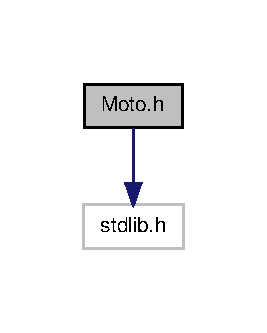
\includegraphics[width=128pt]{_moto_8h__incl}
\end{center}
\end{figure}
Ce graphe montre quels fichiers incluent directement ou indirectement ce fichier \-:\nopagebreak
\begin{figure}[H]
\begin{center}
\leavevmode
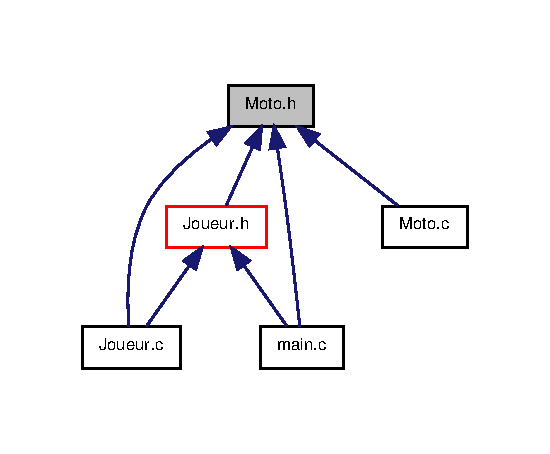
\includegraphics[width=350pt]{_moto_8h__dep__incl}
\end{center}
\end{figure}
\subsection*{Structures de données}
\begin{DoxyCompactItemize}
\item 
struct \hyperlink{struct_moto}{Moto}
\end{DoxyCompactItemize}
\subsection*{Énumérations}
\begin{DoxyCompactItemize}
\item 
enum \hyperlink{_moto_8h_a224b9163917ac32fc95a60d8c1eec3aa}{Direction} \{ \\*
\hyperlink{_moto_8h_a224b9163917ac32fc95a60d8c1eec3aaa63b67464045a0f9f8aece9dfd409ecf8}{N\-O\-N\-\_\-\-D\-I\-R\-I\-G\-E} =0, 
\hyperlink{_moto_8h_a224b9163917ac32fc95a60d8c1eec3aaa5c97701a87d36c8f2c0de80c5865b8e2}{H\-A\-U\-T} =1, 
\hyperlink{_moto_8h_a224b9163917ac32fc95a60d8c1eec3aaa4b07baad9e862178efeac3e522475caa}{B\-A\-S} =2, 
\hyperlink{_moto_8h_a224b9163917ac32fc95a60d8c1eec3aaa4ee960d97b04a1f22ed7ff81c7aa2e86}{G\-A\-U\-C\-H\-E} =3, 
\\*
\hyperlink{_moto_8h_a224b9163917ac32fc95a60d8c1eec3aaa79f680205087956546ae263797bd1343}{D\-R\-O\-I\-T\-E} =4
 \}
\end{DoxyCompactItemize}
\subsection*{Fonctions}
\begin{DoxyCompactItemize}
\item 
float \hyperlink{_moto_8h_a4156c04a753d20234c7882f960830e72}{Moto\-Get\-Position\-X} (const \hyperlink{struct_moto}{Moto} $\ast$moto)
\item 
float \hyperlink{_moto_8h_a62ff0acafab13335eb75daddd0f1b842}{Moto\-Get\-Position\-Y} (const \hyperlink{struct_moto}{Moto} $\ast$moto)
\item 
unsigned int \hyperlink{_moto_8h_a3c4edf672fcff5483b3805ea4850b0bf}{Moto\-Get\-Taille\-X} (const \hyperlink{struct_moto}{Moto} $\ast$moto)
\item 
unsigned int \hyperlink{_moto_8h_aa2e2c249d5453b97bbe5a0a3dcfec6c0}{Moto\-Get\-Taille\-Y} (const \hyperlink{struct_moto}{Moto} $\ast$moto)
\item 
float \hyperlink{_moto_8h_a211ad1ea110f768b154253e64386c999}{Moto\-Get\-Vitesse} (const \hyperlink{struct_moto}{Moto} $\ast$moto)
\item 
\hyperlink{_moto_8h_a224b9163917ac32fc95a60d8c1eec3aa}{Direction} \hyperlink{_moto_8h_a3b507a0e47b0c30898ff385292ad44ba}{Moto\-Get\-Direction} (const \hyperlink{struct_moto}{Moto} $\ast$moto)
\item 
void \hyperlink{_moto_8h_ae7ad014965db768aafd0af24b3594aee}{Moto\-Set\-Position\-X} (\hyperlink{struct_moto}{Moto} $\ast$m, float pos\-X)
\item 
void \hyperlink{_moto_8h_ad295a21e2ee7f293ef9b1e732f5d3c67}{Moto\-Set\-Position\-Y} (\hyperlink{struct_moto}{Moto} $\ast$m, float pos\-Y)
\item 
void \hyperlink{_moto_8h_af0e8990952a6350076e48481a6bb7cb2}{Moto\-Set\-Taille\-X} (\hyperlink{struct_moto}{Moto} $\ast$m, unsigned int taille\-X)
\item 
void \hyperlink{_moto_8h_a8fc03b4457ff37ecd14b7088502625bf}{Moto\-Set\-Taille\-Y} (\hyperlink{struct_moto}{Moto} $\ast$m, unsigned int taille\-Y)
\item 
void \hyperlink{_moto_8h_a94e23a15f224645b6f06456d72238353}{Moto\-Set\-Vitesse} (\hyperlink{struct_moto}{Moto} $\ast$m, float vitesse)
\item 
void \hyperlink{_moto_8h_ae3ad3af0cde9ce8df3c3c25d708e5be9}{Moto\-Set\-Direction} (\hyperlink{struct_moto}{Moto} $\ast$m, \hyperlink{_moto_8h_a224b9163917ac32fc95a60d8c1eec3aa}{Direction} direction)
\item 
void \hyperlink{_moto_8h_adaa34f67eeb029811b895f62c48e1e37}{Moto\-Constructeur} (\hyperlink{struct_moto}{Moto} $\ast$moto, float pos\-X, float pos\-Y, unsigned int taille\-X, unsigned int taille\-Y, float vitesse, \hyperlink{_moto_8h_a224b9163917ac32fc95a60d8c1eec3aa}{Direction} direction)
\item 
void \hyperlink{_moto_8h_a8c1f41e71c00d38b29d1b8ab0e93d542}{Moto\-Destructeur} (\hyperlink{struct_moto}{Moto} $\ast$moto)
\item 
void \hyperlink{_moto_8h_aee18c911ddc26580170985f506538dcb}{Moto\-Test\-Regression} ()
\end{DoxyCompactItemize}


\subsection{Description détaillée}
\mbox{]} Module des Motos du jeu \begin{DoxyAuthor}{Auteur}
\{Antoine.\-C,Matthieu.\-B\} 
\end{DoxyAuthor}
\begin{DoxyVersion}{Version}
0.\-1 
\end{DoxyVersion}
\begin{DoxyDate}{Date}
13 mars 2013 
\end{DoxyDate}


Définition dans le fichier \hyperlink{_moto_8h_source}{Moto.\-h}.



\subsection{Documentation du type de l'énumération}
\hypertarget{_moto_8h_a224b9163917ac32fc95a60d8c1eec3aa}{\index{Moto.\-h@{Moto.\-h}!Direction@{Direction}}
\index{Direction@{Direction}!Moto.h@{Moto.\-h}}
\subsubsection[{Direction}]{\setlength{\rightskip}{0pt plus 5cm}enum {\bf Direction}}}\label{_moto_8h_a224b9163917ac32fc95a60d8c1eec3aa}
\begin{Desc}
\item[Valeurs énumérées]\par
\begin{description}
\index{N\-O\-N\-\_\-\-D\-I\-R\-I\-G\-E@{N\-O\-N\-\_\-\-D\-I\-R\-I\-G\-E}!Moto.\-h@{Moto.\-h}}\index{Moto.\-h@{Moto.\-h}!N\-O\-N\-\_\-\-D\-I\-R\-I\-G\-E@{N\-O\-N\-\_\-\-D\-I\-R\-I\-G\-E}}\item[{\em 
\hypertarget{_moto_8h_a224b9163917ac32fc95a60d8c1eec3aaa63b67464045a0f9f8aece9dfd409ecf8}{N\-O\-N\-\_\-\-D\-I\-R\-I\-G\-E}\label{_moto_8h_a224b9163917ac32fc95a60d8c1eec3aaa63b67464045a0f9f8aece9dfd409ecf8}
}]\index{H\-A\-U\-T@{H\-A\-U\-T}!Moto.\-h@{Moto.\-h}}\index{Moto.\-h@{Moto.\-h}!H\-A\-U\-T@{H\-A\-U\-T}}\item[{\em 
\hypertarget{_moto_8h_a224b9163917ac32fc95a60d8c1eec3aaa5c97701a87d36c8f2c0de80c5865b8e2}{H\-A\-U\-T}\label{_moto_8h_a224b9163917ac32fc95a60d8c1eec3aaa5c97701a87d36c8f2c0de80c5865b8e2}
}]\index{B\-A\-S@{B\-A\-S}!Moto.\-h@{Moto.\-h}}\index{Moto.\-h@{Moto.\-h}!B\-A\-S@{B\-A\-S}}\item[{\em 
\hypertarget{_moto_8h_a224b9163917ac32fc95a60d8c1eec3aaa4b07baad9e862178efeac3e522475caa}{B\-A\-S}\label{_moto_8h_a224b9163917ac32fc95a60d8c1eec3aaa4b07baad9e862178efeac3e522475caa}
}]\index{G\-A\-U\-C\-H\-E@{G\-A\-U\-C\-H\-E}!Moto.\-h@{Moto.\-h}}\index{Moto.\-h@{Moto.\-h}!G\-A\-U\-C\-H\-E@{G\-A\-U\-C\-H\-E}}\item[{\em 
\hypertarget{_moto_8h_a224b9163917ac32fc95a60d8c1eec3aaa4ee960d97b04a1f22ed7ff81c7aa2e86}{G\-A\-U\-C\-H\-E}\label{_moto_8h_a224b9163917ac32fc95a60d8c1eec3aaa4ee960d97b04a1f22ed7ff81c7aa2e86}
}]\index{D\-R\-O\-I\-T\-E@{D\-R\-O\-I\-T\-E}!Moto.\-h@{Moto.\-h}}\index{Moto.\-h@{Moto.\-h}!D\-R\-O\-I\-T\-E@{D\-R\-O\-I\-T\-E}}\item[{\em 
\hypertarget{_moto_8h_a224b9163917ac32fc95a60d8c1eec3aaa79f680205087956546ae263797bd1343}{D\-R\-O\-I\-T\-E}\label{_moto_8h_a224b9163917ac32fc95a60d8c1eec3aaa79f680205087956546ae263797bd1343}
}]\end{description}
\end{Desc}


Définition à la ligne 14 du fichier Moto.\-h.



\subsection{Documentation des fonctions}
\hypertarget{_moto_8h_adaa34f67eeb029811b895f62c48e1e37}{\index{Moto.\-h@{Moto.\-h}!Moto\-Constructeur@{Moto\-Constructeur}}
\index{Moto\-Constructeur@{Moto\-Constructeur}!Moto.h@{Moto.\-h}}
\subsubsection[{Moto\-Constructeur}]{\setlength{\rightskip}{0pt plus 5cm}void Moto\-Constructeur (
\begin{DoxyParamCaption}
\item[{{\bf Moto} $\ast$}]{moto, }
\item[{float}]{pos\-X, }
\item[{float}]{pos\-Y, }
\item[{unsigned int}]{taille\-X, }
\item[{unsigned int}]{taille\-Y, }
\item[{float}]{vitesse, }
\item[{{\bf Direction}}]{direction}
\end{DoxyParamCaption}
)}}\label{_moto_8h_adaa34f67eeb029811b895f62c48e1e37}


Définition à la ligne 51 du fichier Moto.\-c.

\hypertarget{_moto_8h_a8c1f41e71c00d38b29d1b8ab0e93d542}{\index{Moto.\-h@{Moto.\-h}!Moto\-Destructeur@{Moto\-Destructeur}}
\index{Moto\-Destructeur@{Moto\-Destructeur}!Moto.h@{Moto.\-h}}
\subsubsection[{Moto\-Destructeur}]{\setlength{\rightskip}{0pt plus 5cm}void Moto\-Destructeur (
\begin{DoxyParamCaption}
\item[{{\bf Moto} $\ast$}]{moto}
\end{DoxyParamCaption}
)}}\label{_moto_8h_a8c1f41e71c00d38b29d1b8ab0e93d542}


Définition à la ligne 59 du fichier Moto.\-c.

\hypertarget{_moto_8h_a3b507a0e47b0c30898ff385292ad44ba}{\index{Moto.\-h@{Moto.\-h}!Moto\-Get\-Direction@{Moto\-Get\-Direction}}
\index{Moto\-Get\-Direction@{Moto\-Get\-Direction}!Moto.h@{Moto.\-h}}
\subsubsection[{Moto\-Get\-Direction}]{\setlength{\rightskip}{0pt plus 5cm}{\bf Direction} Moto\-Get\-Direction (
\begin{DoxyParamCaption}
\item[{const {\bf Moto} $\ast$}]{moto}
\end{DoxyParamCaption}
)}}\label{_moto_8h_a3b507a0e47b0c30898ff385292ad44ba}


Définition à la ligne 28 du fichier Moto.\-c.

\hypertarget{_moto_8h_a4156c04a753d20234c7882f960830e72}{\index{Moto.\-h@{Moto.\-h}!Moto\-Get\-Position\-X@{Moto\-Get\-Position\-X}}
\index{Moto\-Get\-Position\-X@{Moto\-Get\-Position\-X}!Moto.h@{Moto.\-h}}
\subsubsection[{Moto\-Get\-Position\-X}]{\setlength{\rightskip}{0pt plus 5cm}float Moto\-Get\-Position\-X (
\begin{DoxyParamCaption}
\item[{const {\bf Moto} $\ast$}]{moto}
\end{DoxyParamCaption}
)}}\label{_moto_8h_a4156c04a753d20234c7882f960830e72}


Définition à la ligne 13 du fichier Moto.\-c.

\hypertarget{_moto_8h_a62ff0acafab13335eb75daddd0f1b842}{\index{Moto.\-h@{Moto.\-h}!Moto\-Get\-Position\-Y@{Moto\-Get\-Position\-Y}}
\index{Moto\-Get\-Position\-Y@{Moto\-Get\-Position\-Y}!Moto.h@{Moto.\-h}}
\subsubsection[{Moto\-Get\-Position\-Y}]{\setlength{\rightskip}{0pt plus 5cm}float Moto\-Get\-Position\-Y (
\begin{DoxyParamCaption}
\item[{const {\bf Moto} $\ast$}]{moto}
\end{DoxyParamCaption}
)}}\label{_moto_8h_a62ff0acafab13335eb75daddd0f1b842}


Définition à la ligne 16 du fichier Moto.\-c.

\hypertarget{_moto_8h_a3c4edf672fcff5483b3805ea4850b0bf}{\index{Moto.\-h@{Moto.\-h}!Moto\-Get\-Taille\-X@{Moto\-Get\-Taille\-X}}
\index{Moto\-Get\-Taille\-X@{Moto\-Get\-Taille\-X}!Moto.h@{Moto.\-h}}
\subsubsection[{Moto\-Get\-Taille\-X}]{\setlength{\rightskip}{0pt plus 5cm}unsigned int Moto\-Get\-Taille\-X (
\begin{DoxyParamCaption}
\item[{const {\bf Moto} $\ast$}]{moto}
\end{DoxyParamCaption}
)}}\label{_moto_8h_a3c4edf672fcff5483b3805ea4850b0bf}


Définition à la ligne 19 du fichier Moto.\-c.

\hypertarget{_moto_8h_aa2e2c249d5453b97bbe5a0a3dcfec6c0}{\index{Moto.\-h@{Moto.\-h}!Moto\-Get\-Taille\-Y@{Moto\-Get\-Taille\-Y}}
\index{Moto\-Get\-Taille\-Y@{Moto\-Get\-Taille\-Y}!Moto.h@{Moto.\-h}}
\subsubsection[{Moto\-Get\-Taille\-Y}]{\setlength{\rightskip}{0pt plus 5cm}unsigned int Moto\-Get\-Taille\-Y (
\begin{DoxyParamCaption}
\item[{const {\bf Moto} $\ast$}]{moto}
\end{DoxyParamCaption}
)}}\label{_moto_8h_aa2e2c249d5453b97bbe5a0a3dcfec6c0}


Définition à la ligne 22 du fichier Moto.\-c.

\hypertarget{_moto_8h_a211ad1ea110f768b154253e64386c999}{\index{Moto.\-h@{Moto.\-h}!Moto\-Get\-Vitesse@{Moto\-Get\-Vitesse}}
\index{Moto\-Get\-Vitesse@{Moto\-Get\-Vitesse}!Moto.h@{Moto.\-h}}
\subsubsection[{Moto\-Get\-Vitesse}]{\setlength{\rightskip}{0pt plus 5cm}float Moto\-Get\-Vitesse (
\begin{DoxyParamCaption}
\item[{const {\bf Moto} $\ast$}]{moto}
\end{DoxyParamCaption}
)}}\label{_moto_8h_a211ad1ea110f768b154253e64386c999}


Définition à la ligne 25 du fichier Moto.\-c.

\hypertarget{_moto_8h_ae3ad3af0cde9ce8df3c3c25d708e5be9}{\index{Moto.\-h@{Moto.\-h}!Moto\-Set\-Direction@{Moto\-Set\-Direction}}
\index{Moto\-Set\-Direction@{Moto\-Set\-Direction}!Moto.h@{Moto.\-h}}
\subsubsection[{Moto\-Set\-Direction}]{\setlength{\rightskip}{0pt plus 5cm}void Moto\-Set\-Direction (
\begin{DoxyParamCaption}
\item[{{\bf Moto} $\ast$}]{m, }
\item[{{\bf Direction}}]{direction}
\end{DoxyParamCaption}
)}}\label{_moto_8h_ae3ad3af0cde9ce8df3c3c25d708e5be9}


Définition à la ligne 47 du fichier Moto.\-c.

\hypertarget{_moto_8h_ae7ad014965db768aafd0af24b3594aee}{\index{Moto.\-h@{Moto.\-h}!Moto\-Set\-Position\-X@{Moto\-Set\-Position\-X}}
\index{Moto\-Set\-Position\-X@{Moto\-Set\-Position\-X}!Moto.h@{Moto.\-h}}
\subsubsection[{Moto\-Set\-Position\-X}]{\setlength{\rightskip}{0pt plus 5cm}void Moto\-Set\-Position\-X (
\begin{DoxyParamCaption}
\item[{{\bf Moto} $\ast$}]{m, }
\item[{float}]{pos\-X}
\end{DoxyParamCaption}
)}}\label{_moto_8h_ae7ad014965db768aafd0af24b3594aee}


Définition à la ligne 32 du fichier Moto.\-c.

\hypertarget{_moto_8h_ad295a21e2ee7f293ef9b1e732f5d3c67}{\index{Moto.\-h@{Moto.\-h}!Moto\-Set\-Position\-Y@{Moto\-Set\-Position\-Y}}
\index{Moto\-Set\-Position\-Y@{Moto\-Set\-Position\-Y}!Moto.h@{Moto.\-h}}
\subsubsection[{Moto\-Set\-Position\-Y}]{\setlength{\rightskip}{0pt plus 5cm}void Moto\-Set\-Position\-Y (
\begin{DoxyParamCaption}
\item[{{\bf Moto} $\ast$}]{m, }
\item[{float}]{pos\-Y}
\end{DoxyParamCaption}
)}}\label{_moto_8h_ad295a21e2ee7f293ef9b1e732f5d3c67}


Définition à la ligne 35 du fichier Moto.\-c.

\hypertarget{_moto_8h_af0e8990952a6350076e48481a6bb7cb2}{\index{Moto.\-h@{Moto.\-h}!Moto\-Set\-Taille\-X@{Moto\-Set\-Taille\-X}}
\index{Moto\-Set\-Taille\-X@{Moto\-Set\-Taille\-X}!Moto.h@{Moto.\-h}}
\subsubsection[{Moto\-Set\-Taille\-X}]{\setlength{\rightskip}{0pt plus 5cm}void Moto\-Set\-Taille\-X (
\begin{DoxyParamCaption}
\item[{{\bf Moto} $\ast$}]{m, }
\item[{unsigned int}]{taille\-X}
\end{DoxyParamCaption}
)}}\label{_moto_8h_af0e8990952a6350076e48481a6bb7cb2}


Définition à la ligne 38 du fichier Moto.\-c.

\hypertarget{_moto_8h_a8fc03b4457ff37ecd14b7088502625bf}{\index{Moto.\-h@{Moto.\-h}!Moto\-Set\-Taille\-Y@{Moto\-Set\-Taille\-Y}}
\index{Moto\-Set\-Taille\-Y@{Moto\-Set\-Taille\-Y}!Moto.h@{Moto.\-h}}
\subsubsection[{Moto\-Set\-Taille\-Y}]{\setlength{\rightskip}{0pt plus 5cm}void Moto\-Set\-Taille\-Y (
\begin{DoxyParamCaption}
\item[{{\bf Moto} $\ast$}]{m, }
\item[{unsigned int}]{taille\-Y}
\end{DoxyParamCaption}
)}}\label{_moto_8h_a8fc03b4457ff37ecd14b7088502625bf}


Définition à la ligne 41 du fichier Moto.\-c.

\hypertarget{_moto_8h_a94e23a15f224645b6f06456d72238353}{\index{Moto.\-h@{Moto.\-h}!Moto\-Set\-Vitesse@{Moto\-Set\-Vitesse}}
\index{Moto\-Set\-Vitesse@{Moto\-Set\-Vitesse}!Moto.h@{Moto.\-h}}
\subsubsection[{Moto\-Set\-Vitesse}]{\setlength{\rightskip}{0pt plus 5cm}void Moto\-Set\-Vitesse (
\begin{DoxyParamCaption}
\item[{{\bf Moto} $\ast$}]{m, }
\item[{float}]{vitesse}
\end{DoxyParamCaption}
)}}\label{_moto_8h_a94e23a15f224645b6f06456d72238353}


Définition à la ligne 44 du fichier Moto.\-c.

\hypertarget{_moto_8h_aee18c911ddc26580170985f506538dcb}{\index{Moto.\-h@{Moto.\-h}!Moto\-Test\-Regression@{Moto\-Test\-Regression}}
\index{Moto\-Test\-Regression@{Moto\-Test\-Regression}!Moto.h@{Moto.\-h}}
\subsubsection[{Moto\-Test\-Regression}]{\setlength{\rightskip}{0pt plus 5cm}void Moto\-Test\-Regression (
\begin{DoxyParamCaption}
{}
\end{DoxyParamCaption}
)}}\label{_moto_8h_aee18c911ddc26580170985f506538dcb}


Définition à la ligne 68 du fichier Moto.\-c.


\hypertarget{_mur_8c}{\section{Référence du fichier Mur.\-c}
\label{_mur_8c}\index{Mur.\-c@{Mur.\-c}}
}
{\ttfamily \#include $<$stdlib.\-h$>$}\\*
{\ttfamily \#include $<$stdio.\-h$>$}\\*
{\ttfamily \#include \char`\"{}Couleur.\-h\char`\"{}}\\*
{\ttfamily \#include \char`\"{}Mur.\-h\char`\"{}}\\*
Graphe des dépendances par inclusion de Mur.\-c\-:\nopagebreak
\begin{figure}[H]
\begin{center}
\leavevmode
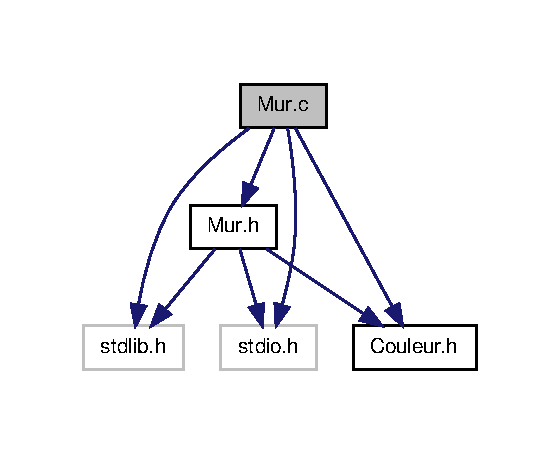
\includegraphics[width=268pt]{_mur_8c__incl}
\end{center}
\end{figure}
\subsection*{Fonctions}
\begin{DoxyCompactItemize}
\item 
float \hyperlink{_mur_8c_a242796bbf2bac8399f38a190f18edfbc}{Mur\-Get\-Position\-X} (const \hyperlink{struct_mur}{Mur} $\ast$mur)
\item 
float \hyperlink{_mur_8c_a97acc9d9bb325986a464ee05db5e6fbe}{Mur\-Get\-Position\-Y} (const \hyperlink{struct_mur}{Mur} $\ast$mur)
\item 
unsigned int \hyperlink{_mur_8c_abeddf3763bcdb728a7e3bac665a64552}{Mur\-Get\-Taille\-X} (const \hyperlink{struct_mur}{Mur} $\ast$mur)
\item 
unsigned int \hyperlink{_mur_8c_ab0f66438f4a38b71a243bad168ee0178}{Mur\-Get\-Taille\-Y} (const \hyperlink{struct_mur}{Mur} $\ast$mur)
\item 
\hyperlink{_couleur_8h_aa304d0ca681f782b1d7735da33037dd7}{Couleur} \hyperlink{_mur_8c_a9b9c7924d6ba7afb0fe4daef7cf58d8d}{Mur\-Get\-Couleur} (const \hyperlink{struct_mur}{Mur} $\ast$mur)
\item 
float \hyperlink{_mur_8c_a0150e2edbf0f0c8a60df0b8c261835e2}{Mur\-Get\-Duree\-Vie} (const \hyperlink{struct_mur}{Mur} $\ast$mur)
\item 
void \hyperlink{_mur_8c_acef090d8aa04a7f2c059113ef5fff387}{Mur\-Set\-Position\-X} (\hyperlink{struct_mur}{Mur} $\ast$mur, float pos\-X)
\item 
void \hyperlink{_mur_8c_a09e4ebc64953687f4887b95204db41e2}{Mur\-Set\-Position\-Y} (\hyperlink{struct_mur}{Mur} $\ast$mur, float pos\-Y)
\item 
void \hyperlink{_mur_8c_a12cb4b9c7117a03037cb836ce53864dc}{Mur\-Set\-Taille\-X} (\hyperlink{struct_mur}{Mur} $\ast$mur, unsigned int taille\-X)
\item 
void \hyperlink{_mur_8c_a0749cb2928457b9738b542c3e83f3176}{Mur\-Set\-Taille\-Y} (\hyperlink{struct_mur}{Mur} $\ast$mur, unsigned int taille\-Y)
\item 
void \hyperlink{_mur_8c_a363d065942b92543a4cd0324531a7aa6}{Mur\-Set\-Couleur} (\hyperlink{struct_mur}{Mur} $\ast$mur, \hyperlink{_couleur_8h_aa304d0ca681f782b1d7735da33037dd7}{Couleur} couleur)
\item 
void \hyperlink{_mur_8c_aec089b77b6955d33c9ce127727593458}{Mur\-Set\-Duree\-Vie} (\hyperlink{struct_mur}{Mur} $\ast$mur, float duree)
\item 
void \hyperlink{_mur_8c_a48159b7842108cf44f51dfba06fae844}{Mur\-Constructeur} (\hyperlink{struct_mur}{Mur} $\ast$mur, float pos\-X, float pos\-Y, unsigned int taille\-X, unsigned int taille\-Y, \hyperlink{_couleur_8h_aa304d0ca681f782b1d7735da33037dd7}{Couleur} couleur, float duree\-Vie)
\item 
void \hyperlink{_mur_8c_a1661630a97686483f104c48fd06dec8e}{Mur\-Destructeur} (\hyperlink{struct_mur}{Mur} $\ast$mur)
\item 
void \hyperlink{_mur_8c_a5b1e2027147808ddbccc9c211f929f9e}{Affiche\-Stats\-Mur} (\hyperlink{struct_mur}{Mur} $\ast$mur)
\item 
void \hyperlink{_mur_8c_af409c42d1dd41eae59e90b0f2c6dae06}{Mur\-Test\-Regression} ()
\end{DoxyCompactItemize}


\subsection{Description détaillée}
\mbox{]} Module des Murs du \hyperlink{struct_jeu}{Jeu} \begin{DoxyAuthor}{Auteur}
\{Antoine.\-C,Matthieu.\-B\} 
\end{DoxyAuthor}
\begin{DoxyVersion}{Version}
0.\-1 
\end{DoxyVersion}
\begin{DoxyDate}{Date}
13 mars 2013 
\end{DoxyDate}


Définition dans le fichier \hyperlink{_mur_8c_source}{Mur.\-c}.



\subsection{Documentation des fonctions}
\hypertarget{_mur_8c_a5b1e2027147808ddbccc9c211f929f9e}{\index{Mur.\-c@{Mur.\-c}!Affiche\-Stats\-Mur@{Affiche\-Stats\-Mur}}
\index{Affiche\-Stats\-Mur@{Affiche\-Stats\-Mur}!Mur.c@{Mur.\-c}}
\subsubsection[{Affiche\-Stats\-Mur}]{\setlength{\rightskip}{0pt plus 5cm}void Affiche\-Stats\-Mur (
\begin{DoxyParamCaption}
\item[{{\bf Mur} $\ast$}]{mur}
\end{DoxyParamCaption}
)}}\label{_mur_8c_a5b1e2027147808ddbccc9c211f929f9e}


Définition à la ligne 68 du fichier Mur.\-c.

\hypertarget{_mur_8c_a48159b7842108cf44f51dfba06fae844}{\index{Mur.\-c@{Mur.\-c}!Mur\-Constructeur@{Mur\-Constructeur}}
\index{Mur\-Constructeur@{Mur\-Constructeur}!Mur.c@{Mur.\-c}}
\subsubsection[{Mur\-Constructeur}]{\setlength{\rightskip}{0pt plus 5cm}void Mur\-Constructeur (
\begin{DoxyParamCaption}
\item[{{\bf Mur} $\ast$}]{mur, }
\item[{float}]{pos\-X, }
\item[{float}]{pos\-Y, }
\item[{unsigned int}]{taille\-X, }
\item[{unsigned int}]{taille\-Y, }
\item[{{\bf Couleur}}]{couleur, }
\item[{float}]{duree\-Vie}
\end{DoxyParamCaption}
)}}\label{_mur_8c_a48159b7842108cf44f51dfba06fae844}


Définition à la ligne 52 du fichier Mur.\-c.

\hypertarget{_mur_8c_a1661630a97686483f104c48fd06dec8e}{\index{Mur.\-c@{Mur.\-c}!Mur\-Destructeur@{Mur\-Destructeur}}
\index{Mur\-Destructeur@{Mur\-Destructeur}!Mur.c@{Mur.\-c}}
\subsubsection[{Mur\-Destructeur}]{\setlength{\rightskip}{0pt plus 5cm}void Mur\-Destructeur (
\begin{DoxyParamCaption}
\item[{{\bf Mur} $\ast$}]{mur}
\end{DoxyParamCaption}
)}}\label{_mur_8c_a1661630a97686483f104c48fd06dec8e}


Définition à la ligne 60 du fichier Mur.\-c.

\hypertarget{_mur_8c_a9b9c7924d6ba7afb0fe4daef7cf58d8d}{\index{Mur.\-c@{Mur.\-c}!Mur\-Get\-Couleur@{Mur\-Get\-Couleur}}
\index{Mur\-Get\-Couleur@{Mur\-Get\-Couleur}!Mur.c@{Mur.\-c}}
\subsubsection[{Mur\-Get\-Couleur}]{\setlength{\rightskip}{0pt plus 5cm}{\bf Couleur} Mur\-Get\-Couleur (
\begin{DoxyParamCaption}
\item[{const {\bf Mur} $\ast$}]{mur}
\end{DoxyParamCaption}
)}}\label{_mur_8c_a9b9c7924d6ba7afb0fe4daef7cf58d8d}


Définition à la ligne 25 du fichier Mur.\-c.

\hypertarget{_mur_8c_a0150e2edbf0f0c8a60df0b8c261835e2}{\index{Mur.\-c@{Mur.\-c}!Mur\-Get\-Duree\-Vie@{Mur\-Get\-Duree\-Vie}}
\index{Mur\-Get\-Duree\-Vie@{Mur\-Get\-Duree\-Vie}!Mur.c@{Mur.\-c}}
\subsubsection[{Mur\-Get\-Duree\-Vie}]{\setlength{\rightskip}{0pt plus 5cm}float Mur\-Get\-Duree\-Vie (
\begin{DoxyParamCaption}
\item[{const {\bf Mur} $\ast$}]{mur}
\end{DoxyParamCaption}
)}}\label{_mur_8c_a0150e2edbf0f0c8a60df0b8c261835e2}


Définition à la ligne 28 du fichier Mur.\-c.

\hypertarget{_mur_8c_a242796bbf2bac8399f38a190f18edfbc}{\index{Mur.\-c@{Mur.\-c}!Mur\-Get\-Position\-X@{Mur\-Get\-Position\-X}}
\index{Mur\-Get\-Position\-X@{Mur\-Get\-Position\-X}!Mur.c@{Mur.\-c}}
\subsubsection[{Mur\-Get\-Position\-X}]{\setlength{\rightskip}{0pt plus 5cm}float Mur\-Get\-Position\-X (
\begin{DoxyParamCaption}
\item[{const {\bf Mur} $\ast$}]{mur}
\end{DoxyParamCaption}
)}}\label{_mur_8c_a242796bbf2bac8399f38a190f18edfbc}


Définition à la ligne 13 du fichier Mur.\-c.

\hypertarget{_mur_8c_a97acc9d9bb325986a464ee05db5e6fbe}{\index{Mur.\-c@{Mur.\-c}!Mur\-Get\-Position\-Y@{Mur\-Get\-Position\-Y}}
\index{Mur\-Get\-Position\-Y@{Mur\-Get\-Position\-Y}!Mur.c@{Mur.\-c}}
\subsubsection[{Mur\-Get\-Position\-Y}]{\setlength{\rightskip}{0pt plus 5cm}float Mur\-Get\-Position\-Y (
\begin{DoxyParamCaption}
\item[{const {\bf Mur} $\ast$}]{mur}
\end{DoxyParamCaption}
)}}\label{_mur_8c_a97acc9d9bb325986a464ee05db5e6fbe}


Définition à la ligne 16 du fichier Mur.\-c.

\hypertarget{_mur_8c_abeddf3763bcdb728a7e3bac665a64552}{\index{Mur.\-c@{Mur.\-c}!Mur\-Get\-Taille\-X@{Mur\-Get\-Taille\-X}}
\index{Mur\-Get\-Taille\-X@{Mur\-Get\-Taille\-X}!Mur.c@{Mur.\-c}}
\subsubsection[{Mur\-Get\-Taille\-X}]{\setlength{\rightskip}{0pt plus 5cm}unsigned int Mur\-Get\-Taille\-X (
\begin{DoxyParamCaption}
\item[{const {\bf Mur} $\ast$}]{mur}
\end{DoxyParamCaption}
)}}\label{_mur_8c_abeddf3763bcdb728a7e3bac665a64552}


Définition à la ligne 19 du fichier Mur.\-c.

\hypertarget{_mur_8c_ab0f66438f4a38b71a243bad168ee0178}{\index{Mur.\-c@{Mur.\-c}!Mur\-Get\-Taille\-Y@{Mur\-Get\-Taille\-Y}}
\index{Mur\-Get\-Taille\-Y@{Mur\-Get\-Taille\-Y}!Mur.c@{Mur.\-c}}
\subsubsection[{Mur\-Get\-Taille\-Y}]{\setlength{\rightskip}{0pt plus 5cm}unsigned int Mur\-Get\-Taille\-Y (
\begin{DoxyParamCaption}
\item[{const {\bf Mur} $\ast$}]{mur}
\end{DoxyParamCaption}
)}}\label{_mur_8c_ab0f66438f4a38b71a243bad168ee0178}


Définition à la ligne 22 du fichier Mur.\-c.

\hypertarget{_mur_8c_a363d065942b92543a4cd0324531a7aa6}{\index{Mur.\-c@{Mur.\-c}!Mur\-Set\-Couleur@{Mur\-Set\-Couleur}}
\index{Mur\-Set\-Couleur@{Mur\-Set\-Couleur}!Mur.c@{Mur.\-c}}
\subsubsection[{Mur\-Set\-Couleur}]{\setlength{\rightskip}{0pt plus 5cm}void Mur\-Set\-Couleur (
\begin{DoxyParamCaption}
\item[{{\bf Mur} $\ast$}]{mur, }
\item[{{\bf Couleur}}]{couleur}
\end{DoxyParamCaption}
)}}\label{_mur_8c_a363d065942b92543a4cd0324531a7aa6}


Définition à la ligne 44 du fichier Mur.\-c.

\hypertarget{_mur_8c_aec089b77b6955d33c9ce127727593458}{\index{Mur.\-c@{Mur.\-c}!Mur\-Set\-Duree\-Vie@{Mur\-Set\-Duree\-Vie}}
\index{Mur\-Set\-Duree\-Vie@{Mur\-Set\-Duree\-Vie}!Mur.c@{Mur.\-c}}
\subsubsection[{Mur\-Set\-Duree\-Vie}]{\setlength{\rightskip}{0pt plus 5cm}void Mur\-Set\-Duree\-Vie (
\begin{DoxyParamCaption}
\item[{{\bf Mur} $\ast$}]{mur, }
\item[{float}]{duree}
\end{DoxyParamCaption}
)}}\label{_mur_8c_aec089b77b6955d33c9ce127727593458}


Définition à la ligne 47 du fichier Mur.\-c.

\hypertarget{_mur_8c_acef090d8aa04a7f2c059113ef5fff387}{\index{Mur.\-c@{Mur.\-c}!Mur\-Set\-Position\-X@{Mur\-Set\-Position\-X}}
\index{Mur\-Set\-Position\-X@{Mur\-Set\-Position\-X}!Mur.c@{Mur.\-c}}
\subsubsection[{Mur\-Set\-Position\-X}]{\setlength{\rightskip}{0pt plus 5cm}void Mur\-Set\-Position\-X (
\begin{DoxyParamCaption}
\item[{{\bf Mur} $\ast$}]{mur, }
\item[{float}]{pos\-X}
\end{DoxyParamCaption}
)}}\label{_mur_8c_acef090d8aa04a7f2c059113ef5fff387}


Définition à la ligne 32 du fichier Mur.\-c.

\hypertarget{_mur_8c_a09e4ebc64953687f4887b95204db41e2}{\index{Mur.\-c@{Mur.\-c}!Mur\-Set\-Position\-Y@{Mur\-Set\-Position\-Y}}
\index{Mur\-Set\-Position\-Y@{Mur\-Set\-Position\-Y}!Mur.c@{Mur.\-c}}
\subsubsection[{Mur\-Set\-Position\-Y}]{\setlength{\rightskip}{0pt plus 5cm}void Mur\-Set\-Position\-Y (
\begin{DoxyParamCaption}
\item[{{\bf Mur} $\ast$}]{mur, }
\item[{float}]{pos\-Y}
\end{DoxyParamCaption}
)}}\label{_mur_8c_a09e4ebc64953687f4887b95204db41e2}


Définition à la ligne 35 du fichier Mur.\-c.

\hypertarget{_mur_8c_a12cb4b9c7117a03037cb836ce53864dc}{\index{Mur.\-c@{Mur.\-c}!Mur\-Set\-Taille\-X@{Mur\-Set\-Taille\-X}}
\index{Mur\-Set\-Taille\-X@{Mur\-Set\-Taille\-X}!Mur.c@{Mur.\-c}}
\subsubsection[{Mur\-Set\-Taille\-X}]{\setlength{\rightskip}{0pt plus 5cm}void Mur\-Set\-Taille\-X (
\begin{DoxyParamCaption}
\item[{{\bf Mur} $\ast$}]{mur, }
\item[{unsigned int}]{taille\-X}
\end{DoxyParamCaption}
)}}\label{_mur_8c_a12cb4b9c7117a03037cb836ce53864dc}


Définition à la ligne 38 du fichier Mur.\-c.

\hypertarget{_mur_8c_a0749cb2928457b9738b542c3e83f3176}{\index{Mur.\-c@{Mur.\-c}!Mur\-Set\-Taille\-Y@{Mur\-Set\-Taille\-Y}}
\index{Mur\-Set\-Taille\-Y@{Mur\-Set\-Taille\-Y}!Mur.c@{Mur.\-c}}
\subsubsection[{Mur\-Set\-Taille\-Y}]{\setlength{\rightskip}{0pt plus 5cm}void Mur\-Set\-Taille\-Y (
\begin{DoxyParamCaption}
\item[{{\bf Mur} $\ast$}]{mur, }
\item[{unsigned int}]{taille\-Y}
\end{DoxyParamCaption}
)}}\label{_mur_8c_a0749cb2928457b9738b542c3e83f3176}


Définition à la ligne 41 du fichier Mur.\-c.

\hypertarget{_mur_8c_af409c42d1dd41eae59e90b0f2c6dae06}{\index{Mur.\-c@{Mur.\-c}!Mur\-Test\-Regression@{Mur\-Test\-Regression}}
\index{Mur\-Test\-Regression@{Mur\-Test\-Regression}!Mur.c@{Mur.\-c}}
\subsubsection[{Mur\-Test\-Regression}]{\setlength{\rightskip}{0pt plus 5cm}Mur\-Test\-Regression (
\begin{DoxyParamCaption}
{}
\end{DoxyParamCaption}
)}}\label{_mur_8c_af409c42d1dd41eae59e90b0f2c6dae06}
Procédure qui teste le Module 

Définition à la ligne 76 du fichier Mur.\-c.


\hypertarget{_mur_8h}{\section{Référence du fichier Mur.\-h}
\label{_mur_8h}\index{Mur.\-h@{Mur.\-h}}
}
{\ttfamily \#include $<$stdlib.\-h$>$}\\*
{\ttfamily \#include $<$stdio.\-h$>$}\\*
{\ttfamily \#include \char`\"{}Couleur.\-h\char`\"{}}\\*
Graphe des dépendances par inclusion de Mur.\-h\-:\nopagebreak
\begin{figure}[H]
\begin{center}
\leavevmode
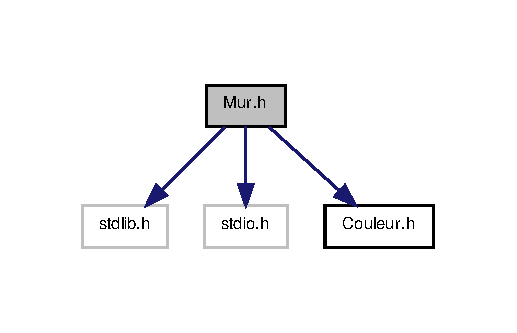
\includegraphics[width=268pt]{_mur_8h__incl}
\end{center}
\end{figure}
Ce graphe montre quels fichiers incluent directement ou indirectement ce fichier \-:\nopagebreak
\begin{figure}[H]
\begin{center}
\leavevmode
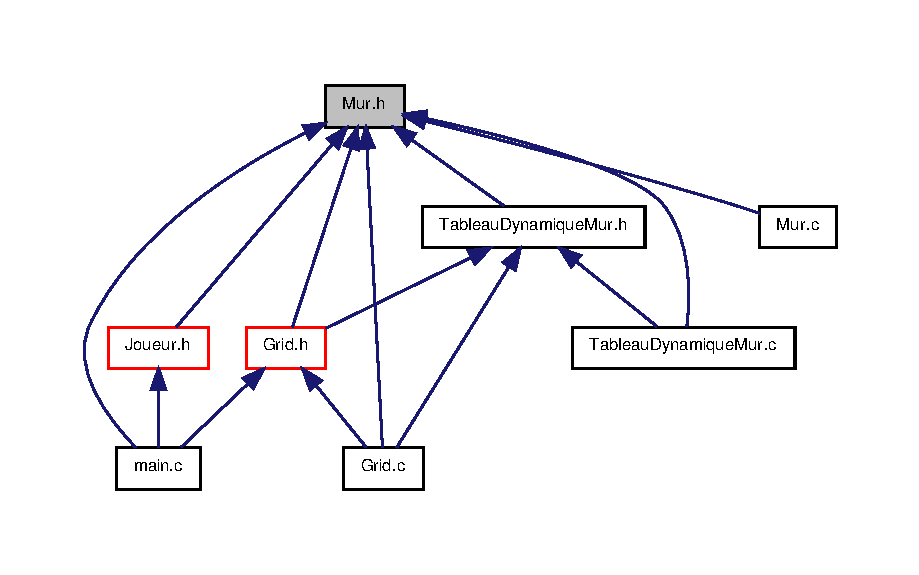
\includegraphics[width=350pt]{_mur_8h__dep__incl}
\end{center}
\end{figure}
\subsection*{Structures de données}
\begin{DoxyCompactItemize}
\item 
struct \hyperlink{struct_mur}{Mur}
\end{DoxyCompactItemize}
\subsection*{Fonctions}
\begin{DoxyCompactItemize}
\item 
float \hyperlink{_mur_8h_a242796bbf2bac8399f38a190f18edfbc}{Mur\-Get\-Position\-X} (const \hyperlink{struct_mur}{Mur} $\ast$mur)
\item 
float \hyperlink{_mur_8h_a97acc9d9bb325986a464ee05db5e6fbe}{Mur\-Get\-Position\-Y} (const \hyperlink{struct_mur}{Mur} $\ast$mur)
\item 
unsigned int \hyperlink{_mur_8h_abeddf3763bcdb728a7e3bac665a64552}{Mur\-Get\-Taille\-X} (const \hyperlink{struct_mur}{Mur} $\ast$mur)
\item 
unsigned int \hyperlink{_mur_8h_ab0f66438f4a38b71a243bad168ee0178}{Mur\-Get\-Taille\-Y} (const \hyperlink{struct_mur}{Mur} $\ast$mur)
\item 
\hyperlink{_couleur_8h_aa304d0ca681f782b1d7735da33037dd7}{Couleur} \hyperlink{_mur_8h_a9b9c7924d6ba7afb0fe4daef7cf58d8d}{Mur\-Get\-Couleur} (const \hyperlink{struct_mur}{Mur} $\ast$mur)
\item 
float \hyperlink{_mur_8h_a0150e2edbf0f0c8a60df0b8c261835e2}{Mur\-Get\-Duree\-Vie} (const \hyperlink{struct_mur}{Mur} $\ast$mur)
\item 
void \hyperlink{_mur_8h_acef090d8aa04a7f2c059113ef5fff387}{Mur\-Set\-Position\-X} (\hyperlink{struct_mur}{Mur} $\ast$mur, float pos\-X)
\item 
void \hyperlink{_mur_8h_a09e4ebc64953687f4887b95204db41e2}{Mur\-Set\-Position\-Y} (\hyperlink{struct_mur}{Mur} $\ast$mur, float pos\-Y)
\item 
void \hyperlink{_mur_8h_a12cb4b9c7117a03037cb836ce53864dc}{Mur\-Set\-Taille\-X} (\hyperlink{struct_mur}{Mur} $\ast$mur, unsigned int taille\-X)
\item 
void \hyperlink{_mur_8h_a0749cb2928457b9738b542c3e83f3176}{Mur\-Set\-Taille\-Y} (\hyperlink{struct_mur}{Mur} $\ast$mur, unsigned int taille\-Y)
\item 
void \hyperlink{_mur_8h_a363d065942b92543a4cd0324531a7aa6}{Mur\-Set\-Couleur} (\hyperlink{struct_mur}{Mur} $\ast$mur, \hyperlink{_couleur_8h_aa304d0ca681f782b1d7735da33037dd7}{Couleur} couleur)
\item 
void \hyperlink{_mur_8h_a7c8ffaab1a81e082767ee865573f6813}{Mur\-Set\-Duree\-Vie} (\hyperlink{struct_mur}{Mur} $\ast$mur, float duree\-Vie)
\item 
void \hyperlink{_mur_8h_a5b1e2027147808ddbccc9c211f929f9e}{Affiche\-Stats\-Mur} (\hyperlink{struct_mur}{Mur} $\ast$mur)
\item 
void \hyperlink{_mur_8h_a48159b7842108cf44f51dfba06fae844}{Mur\-Constructeur} (\hyperlink{struct_mur}{Mur} $\ast$mur, float pos\-X, float pos\-Y, unsigned int taille\-X, unsigned int taille\-Y, \hyperlink{_couleur_8h_aa304d0ca681f782b1d7735da33037dd7}{Couleur} couleur, float duree\-Vie)
\item 
void \hyperlink{_mur_8h_a1661630a97686483f104c48fd06dec8e}{Mur\-Destructeur} (\hyperlink{struct_mur}{Mur} $\ast$mur)
\item 
void \hyperlink{_mur_8h_ac8810857667a124157a1143ad96c2435}{Mur\-Test\-Regression} ()
\end{DoxyCompactItemize}


\subsection{Description détaillée}
\mbox{]} Module des Murs du \hyperlink{struct_jeu}{Jeu} \begin{DoxyAuthor}{Auteur}
\{Antoine.\-C,Matthieu.\-B\} 
\end{DoxyAuthor}
\begin{DoxyVersion}{Version}
0.\-1 
\end{DoxyVersion}
\begin{DoxyDate}{Date}
13 mars 2013 
\end{DoxyDate}


Définition dans le fichier \hyperlink{_mur_8h_source}{Mur.\-h}.



\subsection{Documentation des fonctions}
\hypertarget{_mur_8h_a5b1e2027147808ddbccc9c211f929f9e}{\index{Mur.\-h@{Mur.\-h}!Affiche\-Stats\-Mur@{Affiche\-Stats\-Mur}}
\index{Affiche\-Stats\-Mur@{Affiche\-Stats\-Mur}!Mur.h@{Mur.\-h}}
\subsubsection[{Affiche\-Stats\-Mur}]{\setlength{\rightskip}{0pt plus 5cm}void Affiche\-Stats\-Mur (
\begin{DoxyParamCaption}
\item[{{\bf Mur} $\ast$}]{mur}
\end{DoxyParamCaption}
)}}\label{_mur_8h_a5b1e2027147808ddbccc9c211f929f9e}


Définition à la ligne 68 du fichier Mur.\-c.

\hypertarget{_mur_8h_a48159b7842108cf44f51dfba06fae844}{\index{Mur.\-h@{Mur.\-h}!Mur\-Constructeur@{Mur\-Constructeur}}
\index{Mur\-Constructeur@{Mur\-Constructeur}!Mur.h@{Mur.\-h}}
\subsubsection[{Mur\-Constructeur}]{\setlength{\rightskip}{0pt plus 5cm}void Mur\-Constructeur (
\begin{DoxyParamCaption}
\item[{{\bf Mur} $\ast$}]{mur, }
\item[{float}]{pos\-X, }
\item[{float}]{pos\-Y, }
\item[{unsigned int}]{taille\-X, }
\item[{unsigned int}]{taille\-Y, }
\item[{{\bf Couleur}}]{couleur, }
\item[{float}]{duree\-Vie}
\end{DoxyParamCaption}
)}}\label{_mur_8h_a48159b7842108cf44f51dfba06fae844}


Définition à la ligne 52 du fichier Mur.\-c.

\hypertarget{_mur_8h_a1661630a97686483f104c48fd06dec8e}{\index{Mur.\-h@{Mur.\-h}!Mur\-Destructeur@{Mur\-Destructeur}}
\index{Mur\-Destructeur@{Mur\-Destructeur}!Mur.h@{Mur.\-h}}
\subsubsection[{Mur\-Destructeur}]{\setlength{\rightskip}{0pt plus 5cm}void Mur\-Destructeur (
\begin{DoxyParamCaption}
\item[{{\bf Mur} $\ast$}]{mur}
\end{DoxyParamCaption}
)}}\label{_mur_8h_a1661630a97686483f104c48fd06dec8e}


Définition à la ligne 60 du fichier Mur.\-c.

\hypertarget{_mur_8h_a9b9c7924d6ba7afb0fe4daef7cf58d8d}{\index{Mur.\-h@{Mur.\-h}!Mur\-Get\-Couleur@{Mur\-Get\-Couleur}}
\index{Mur\-Get\-Couleur@{Mur\-Get\-Couleur}!Mur.h@{Mur.\-h}}
\subsubsection[{Mur\-Get\-Couleur}]{\setlength{\rightskip}{0pt plus 5cm}{\bf Couleur} Mur\-Get\-Couleur (
\begin{DoxyParamCaption}
\item[{const {\bf Mur} $\ast$}]{mur}
\end{DoxyParamCaption}
)}}\label{_mur_8h_a9b9c7924d6ba7afb0fe4daef7cf58d8d}


Définition à la ligne 25 du fichier Mur.\-c.

\hypertarget{_mur_8h_a0150e2edbf0f0c8a60df0b8c261835e2}{\index{Mur.\-h@{Mur.\-h}!Mur\-Get\-Duree\-Vie@{Mur\-Get\-Duree\-Vie}}
\index{Mur\-Get\-Duree\-Vie@{Mur\-Get\-Duree\-Vie}!Mur.h@{Mur.\-h}}
\subsubsection[{Mur\-Get\-Duree\-Vie}]{\setlength{\rightskip}{0pt plus 5cm}float Mur\-Get\-Duree\-Vie (
\begin{DoxyParamCaption}
\item[{const {\bf Mur} $\ast$}]{mur}
\end{DoxyParamCaption}
)}}\label{_mur_8h_a0150e2edbf0f0c8a60df0b8c261835e2}


Définition à la ligne 28 du fichier Mur.\-c.

\hypertarget{_mur_8h_a242796bbf2bac8399f38a190f18edfbc}{\index{Mur.\-h@{Mur.\-h}!Mur\-Get\-Position\-X@{Mur\-Get\-Position\-X}}
\index{Mur\-Get\-Position\-X@{Mur\-Get\-Position\-X}!Mur.h@{Mur.\-h}}
\subsubsection[{Mur\-Get\-Position\-X}]{\setlength{\rightskip}{0pt plus 5cm}float Mur\-Get\-Position\-X (
\begin{DoxyParamCaption}
\item[{const {\bf Mur} $\ast$}]{mur}
\end{DoxyParamCaption}
)}}\label{_mur_8h_a242796bbf2bac8399f38a190f18edfbc}


Définition à la ligne 13 du fichier Mur.\-c.

\hypertarget{_mur_8h_a97acc9d9bb325986a464ee05db5e6fbe}{\index{Mur.\-h@{Mur.\-h}!Mur\-Get\-Position\-Y@{Mur\-Get\-Position\-Y}}
\index{Mur\-Get\-Position\-Y@{Mur\-Get\-Position\-Y}!Mur.h@{Mur.\-h}}
\subsubsection[{Mur\-Get\-Position\-Y}]{\setlength{\rightskip}{0pt plus 5cm}float Mur\-Get\-Position\-Y (
\begin{DoxyParamCaption}
\item[{const {\bf Mur} $\ast$}]{mur}
\end{DoxyParamCaption}
)}}\label{_mur_8h_a97acc9d9bb325986a464ee05db5e6fbe}


Définition à la ligne 16 du fichier Mur.\-c.

\hypertarget{_mur_8h_abeddf3763bcdb728a7e3bac665a64552}{\index{Mur.\-h@{Mur.\-h}!Mur\-Get\-Taille\-X@{Mur\-Get\-Taille\-X}}
\index{Mur\-Get\-Taille\-X@{Mur\-Get\-Taille\-X}!Mur.h@{Mur.\-h}}
\subsubsection[{Mur\-Get\-Taille\-X}]{\setlength{\rightskip}{0pt plus 5cm}unsigned int Mur\-Get\-Taille\-X (
\begin{DoxyParamCaption}
\item[{const {\bf Mur} $\ast$}]{mur}
\end{DoxyParamCaption}
)}}\label{_mur_8h_abeddf3763bcdb728a7e3bac665a64552}


Définition à la ligne 19 du fichier Mur.\-c.

\hypertarget{_mur_8h_ab0f66438f4a38b71a243bad168ee0178}{\index{Mur.\-h@{Mur.\-h}!Mur\-Get\-Taille\-Y@{Mur\-Get\-Taille\-Y}}
\index{Mur\-Get\-Taille\-Y@{Mur\-Get\-Taille\-Y}!Mur.h@{Mur.\-h}}
\subsubsection[{Mur\-Get\-Taille\-Y}]{\setlength{\rightskip}{0pt plus 5cm}unsigned int Mur\-Get\-Taille\-Y (
\begin{DoxyParamCaption}
\item[{const {\bf Mur} $\ast$}]{mur}
\end{DoxyParamCaption}
)}}\label{_mur_8h_ab0f66438f4a38b71a243bad168ee0178}


Définition à la ligne 22 du fichier Mur.\-c.

\hypertarget{_mur_8h_a363d065942b92543a4cd0324531a7aa6}{\index{Mur.\-h@{Mur.\-h}!Mur\-Set\-Couleur@{Mur\-Set\-Couleur}}
\index{Mur\-Set\-Couleur@{Mur\-Set\-Couleur}!Mur.h@{Mur.\-h}}
\subsubsection[{Mur\-Set\-Couleur}]{\setlength{\rightskip}{0pt plus 5cm}void Mur\-Set\-Couleur (
\begin{DoxyParamCaption}
\item[{{\bf Mur} $\ast$}]{mur, }
\item[{{\bf Couleur}}]{couleur}
\end{DoxyParamCaption}
)}}\label{_mur_8h_a363d065942b92543a4cd0324531a7aa6}


Définition à la ligne 44 du fichier Mur.\-c.

\hypertarget{_mur_8h_a7c8ffaab1a81e082767ee865573f6813}{\index{Mur.\-h@{Mur.\-h}!Mur\-Set\-Duree\-Vie@{Mur\-Set\-Duree\-Vie}}
\index{Mur\-Set\-Duree\-Vie@{Mur\-Set\-Duree\-Vie}!Mur.h@{Mur.\-h}}
\subsubsection[{Mur\-Set\-Duree\-Vie}]{\setlength{\rightskip}{0pt plus 5cm}void Mur\-Set\-Duree\-Vie (
\begin{DoxyParamCaption}
\item[{{\bf Mur} $\ast$}]{mur, }
\item[{float}]{duree\-Vie}
\end{DoxyParamCaption}
)}}\label{_mur_8h_a7c8ffaab1a81e082767ee865573f6813}


Définition à la ligne 47 du fichier Mur.\-c.

\hypertarget{_mur_8h_acef090d8aa04a7f2c059113ef5fff387}{\index{Mur.\-h@{Mur.\-h}!Mur\-Set\-Position\-X@{Mur\-Set\-Position\-X}}
\index{Mur\-Set\-Position\-X@{Mur\-Set\-Position\-X}!Mur.h@{Mur.\-h}}
\subsubsection[{Mur\-Set\-Position\-X}]{\setlength{\rightskip}{0pt plus 5cm}void Mur\-Set\-Position\-X (
\begin{DoxyParamCaption}
\item[{{\bf Mur} $\ast$}]{mur, }
\item[{float}]{pos\-X}
\end{DoxyParamCaption}
)}}\label{_mur_8h_acef090d8aa04a7f2c059113ef5fff387}


Définition à la ligne 32 du fichier Mur.\-c.

\hypertarget{_mur_8h_a09e4ebc64953687f4887b95204db41e2}{\index{Mur.\-h@{Mur.\-h}!Mur\-Set\-Position\-Y@{Mur\-Set\-Position\-Y}}
\index{Mur\-Set\-Position\-Y@{Mur\-Set\-Position\-Y}!Mur.h@{Mur.\-h}}
\subsubsection[{Mur\-Set\-Position\-Y}]{\setlength{\rightskip}{0pt plus 5cm}void Mur\-Set\-Position\-Y (
\begin{DoxyParamCaption}
\item[{{\bf Mur} $\ast$}]{mur, }
\item[{float}]{pos\-Y}
\end{DoxyParamCaption}
)}}\label{_mur_8h_a09e4ebc64953687f4887b95204db41e2}


Définition à la ligne 35 du fichier Mur.\-c.

\hypertarget{_mur_8h_a12cb4b9c7117a03037cb836ce53864dc}{\index{Mur.\-h@{Mur.\-h}!Mur\-Set\-Taille\-X@{Mur\-Set\-Taille\-X}}
\index{Mur\-Set\-Taille\-X@{Mur\-Set\-Taille\-X}!Mur.h@{Mur.\-h}}
\subsubsection[{Mur\-Set\-Taille\-X}]{\setlength{\rightskip}{0pt plus 5cm}void Mur\-Set\-Taille\-X (
\begin{DoxyParamCaption}
\item[{{\bf Mur} $\ast$}]{mur, }
\item[{unsigned int}]{taille\-X}
\end{DoxyParamCaption}
)}}\label{_mur_8h_a12cb4b9c7117a03037cb836ce53864dc}


Définition à la ligne 38 du fichier Mur.\-c.

\hypertarget{_mur_8h_a0749cb2928457b9738b542c3e83f3176}{\index{Mur.\-h@{Mur.\-h}!Mur\-Set\-Taille\-Y@{Mur\-Set\-Taille\-Y}}
\index{Mur\-Set\-Taille\-Y@{Mur\-Set\-Taille\-Y}!Mur.h@{Mur.\-h}}
\subsubsection[{Mur\-Set\-Taille\-Y}]{\setlength{\rightskip}{0pt plus 5cm}void Mur\-Set\-Taille\-Y (
\begin{DoxyParamCaption}
\item[{{\bf Mur} $\ast$}]{mur, }
\item[{unsigned int}]{taille\-Y}
\end{DoxyParamCaption}
)}}\label{_mur_8h_a0749cb2928457b9738b542c3e83f3176}


Définition à la ligne 41 du fichier Mur.\-c.

\hypertarget{_mur_8h_ac8810857667a124157a1143ad96c2435}{\index{Mur.\-h@{Mur.\-h}!Mur\-Test\-Regression@{Mur\-Test\-Regression}}
\index{Mur\-Test\-Regression@{Mur\-Test\-Regression}!Mur.h@{Mur.\-h}}
\subsubsection[{Mur\-Test\-Regression}]{\setlength{\rightskip}{0pt plus 5cm}void Mur\-Test\-Regression (
\begin{DoxyParamCaption}
{}
\end{DoxyParamCaption}
)}}\label{_mur_8h_ac8810857667a124157a1143ad96c2435}
Procédure qui teste le Module 

Définition à la ligne 76 du fichier Mur.\-c.


\hypertarget{_musique_8c}{\section{Référence du fichier Musique.\-c}
\label{_musique_8c}\index{Musique.\-c@{Musique.\-c}}
}
{\ttfamily \#include $<$stdio.\-h$>$}\\*
{\ttfamily \#include $<$stdlib.\-h$>$}\\*
{\ttfamily \#include \char`\"{}Musique.\-h\char`\"{}}\\*
{\ttfamily \#include \char`\"{}../lib/\-F\-M\-O\-D/inc/fmod.\-h\char`\"{}}\\*
{\ttfamily \#include \char`\"{}Constantes.\-h\char`\"{}}\\*
Graphe des dépendances par inclusion de Musique.\-c\-:\nopagebreak
\begin{figure}[H]
\begin{center}
\leavevmode
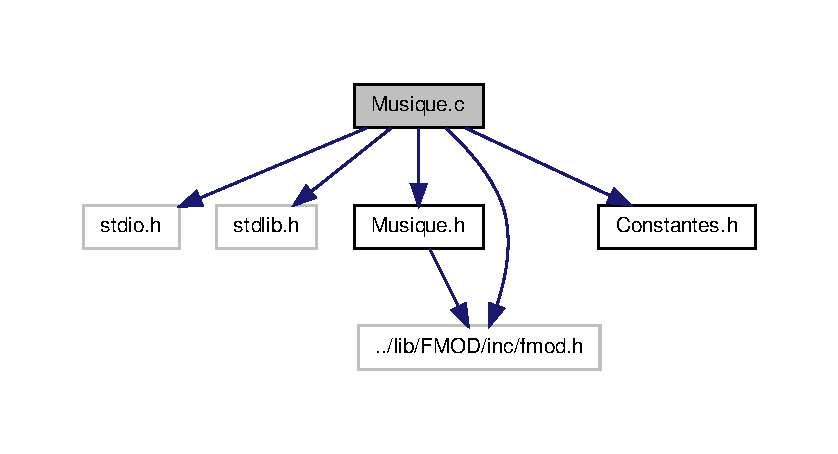
\includegraphics[width=350pt]{_musique_8c__incl}
\end{center}
\end{figure}
\subsection*{Fonctions}
\begin{DoxyCompactItemize}
\item 
F\-M\-O\-D\-\_\-\-S\-Y\-S\-T\-E\-M $\ast$ \hyperlink{_musique_8c_a6eaeb9c1618c807754684d59992d6507}{Musique\-Get\-Base\-Du\-Son} (\hyperlink{struct_musique}{Musique} $\ast$musique)
\item 
F\-M\-O\-D\-\_\-\-S\-O\-U\-N\-D $\ast$ \hyperlink{_musique_8c_af2564aa22a9d674e780a820a9cf2b328}{Musique\-Get\-Ieme\-Son\-Court} (\hyperlink{struct_musique}{Musique} $\ast$musique, int i)
\item 
F\-M\-O\-D\-\_\-\-S\-O\-U\-N\-D $\ast$ \hyperlink{_musique_8c_ada630365fea1e238fbf95631dd56ee49}{Musique\-Get\-Ieme\-Musique\-Du\-Jeu} (\hyperlink{struct_musique}{Musique} $\ast$musique, int i)
\item 
void \hyperlink{_musique_8c_a992e9a70c659319a675744a0bca3799d}{Musique\-Set\-Base\-Du\-Son} (\hyperlink{struct_musique}{Musique} $\ast$musique, F\-M\-O\-D\-\_\-\-S\-Y\-S\-T\-E\-M $\ast$base\-Du\-Son)
\item 
void \hyperlink{_musique_8c_a8126a2d49c47a2dd7ad8c484d01013ad}{Musique\-Set\-Ieme\-Son\-Court} (\hyperlink{struct_musique}{Musique} $\ast$musique, F\-M\-O\-D\-\_\-\-S\-O\-U\-N\-D $\ast$un\-Son, int i)
\item 
void \hyperlink{_musique_8c_adf596c7e8e14980256f0fc5c4cd23a73}{Musique\-Set\-Son\-Court} (\hyperlink{struct_musique}{Musique} $\ast$musique, F\-M\-O\-D\-\_\-\-S\-O\-U\-N\-D $\ast$$\ast$Son\-Court)
\item 
void \hyperlink{_musique_8c_a046f5f78ceaa10d2f8337c53ce976b22}{Musique\-Set\-Ieme\-Musique\-Du\-Jeu} (\hyperlink{struct_musique}{Musique} $\ast$musique, F\-M\-O\-D\-\_\-\-S\-O\-U\-N\-D $\ast$un\-Son, int i)
\item 
void \hyperlink{_musique_8c_aeec5162b4d8bc7da44ce55cfc364015e}{Musique\-Set\-Musique\-Du\-Jeu} (\hyperlink{struct_musique}{Musique} $\ast$musique, F\-M\-O\-D\-\_\-\-S\-O\-U\-N\-D $\ast$$\ast$musique\-Du\-Jeu)
\item 
void \hyperlink{_musique_8c_a43c750ce46e1cebd1d15d08216546b41}{Musique\-Constructeur} (\hyperlink{struct_musique}{Musique} $\ast$musique)
\item 
void \hyperlink{_musique_8c_a968015ab08fbe91eb20129567bb467bc}{Musique\-Destructeur} (\hyperlink{struct_musique}{Musique} $\ast$musique)
\item 
void \hyperlink{_musique_8c_a4ccf3ce1bf3c2fb7ee0ed6352e24fdf4}{Jouer\-Ieme\-Son\-Court} (\hyperlink{struct_musique}{Musique} $\ast$musique, int i)
\item 
void \hyperlink{_musique_8c_a83de1e788ada978f55d7d8442a3beaa8}{Jouer\-Ieme\-Musique} (\hyperlink{struct_musique}{Musique} $\ast$musique, int i, int repetition)
\item 
void \hyperlink{_musique_8c_a3565d4a60201640c1e28cc896d002164}{Musique\-Test\-Regression} ()
\end{DoxyCompactItemize}


\subsection{Description détaillée}
\mbox{]} Module des Musiques du jeu \begin{DoxyAuthor}{Auteur}
\{Antoine.\-C,Matthieu.\-B\} 
\end{DoxyAuthor}
\begin{DoxyVersion}{Version}
1.\-4 
\end{DoxyVersion}
\begin{DoxyDate}{Date}
19 avril 2013 
\end{DoxyDate}


Définition dans le fichier \hyperlink{_musique_8c_source}{Musique.\-c}.



\subsection{Documentation des fonctions}
\hypertarget{_musique_8c_a83de1e788ada978f55d7d8442a3beaa8}{\index{Musique.\-c@{Musique.\-c}!Jouer\-Ieme\-Musique@{Jouer\-Ieme\-Musique}}
\index{Jouer\-Ieme\-Musique@{Jouer\-Ieme\-Musique}!Musique.c@{Musique.\-c}}
\subsubsection[{Jouer\-Ieme\-Musique}]{\setlength{\rightskip}{0pt plus 5cm}void Jouer\-Ieme\-Musique (
\begin{DoxyParamCaption}
\item[{{\bf Musique} $\ast$}]{musique, }
\item[{int}]{i, }
\item[{int}]{repetition}
\end{DoxyParamCaption}
)}}\label{_musique_8c_a83de1e788ada978f55d7d8442a3beaa8}


Définition à la ligne 84 du fichier Musique.\-c.

\hypertarget{_musique_8c_a4ccf3ce1bf3c2fb7ee0ed6352e24fdf4}{\index{Musique.\-c@{Musique.\-c}!Jouer\-Ieme\-Son\-Court@{Jouer\-Ieme\-Son\-Court}}
\index{Jouer\-Ieme\-Son\-Court@{Jouer\-Ieme\-Son\-Court}!Musique.c@{Musique.\-c}}
\subsubsection[{Jouer\-Ieme\-Son\-Court}]{\setlength{\rightskip}{0pt plus 5cm}void Jouer\-Ieme\-Son\-Court (
\begin{DoxyParamCaption}
\item[{{\bf Musique} $\ast$}]{musique, }
\item[{int}]{i}
\end{DoxyParamCaption}
)}}\label{_musique_8c_a4ccf3ce1bf3c2fb7ee0ed6352e24fdf4}


Définition à la ligne 81 du fichier Musique.\-c.

\hypertarget{_musique_8c_a43c750ce46e1cebd1d15d08216546b41}{\index{Musique.\-c@{Musique.\-c}!Musique\-Constructeur@{Musique\-Constructeur}}
\index{Musique\-Constructeur@{Musique\-Constructeur}!Musique.c@{Musique.\-c}}
\subsubsection[{Musique\-Constructeur}]{\setlength{\rightskip}{0pt plus 5cm}void Musique\-Constructeur (
\begin{DoxyParamCaption}
\item[{{\bf Musique} $\ast$}]{musique}
\end{DoxyParamCaption}
)}}\label{_musique_8c_a43c750ce46e1cebd1d15d08216546b41}


Définition à la ligne 44 du fichier Musique.\-c.

\hypertarget{_musique_8c_a968015ab08fbe91eb20129567bb467bc}{\index{Musique.\-c@{Musique.\-c}!Musique\-Destructeur@{Musique\-Destructeur}}
\index{Musique\-Destructeur@{Musique\-Destructeur}!Musique.c@{Musique.\-c}}
\subsubsection[{Musique\-Destructeur}]{\setlength{\rightskip}{0pt plus 5cm}void Musique\-Destructeur (
\begin{DoxyParamCaption}
\item[{{\bf Musique} $\ast$}]{musique}
\end{DoxyParamCaption}
)}}\label{_musique_8c_a968015ab08fbe91eb20129567bb467bc}


Définition à la ligne 67 du fichier Musique.\-c.

\hypertarget{_musique_8c_a6eaeb9c1618c807754684d59992d6507}{\index{Musique.\-c@{Musique.\-c}!Musique\-Get\-Base\-Du\-Son@{Musique\-Get\-Base\-Du\-Son}}
\index{Musique\-Get\-Base\-Du\-Son@{Musique\-Get\-Base\-Du\-Son}!Musique.c@{Musique.\-c}}
\subsubsection[{Musique\-Get\-Base\-Du\-Son}]{\setlength{\rightskip}{0pt plus 5cm}F\-M\-O\-D\-\_\-\-S\-Y\-S\-T\-E\-M$\ast$ Musique\-Get\-Base\-Du\-Son (
\begin{DoxyParamCaption}
\item[{{\bf Musique} $\ast$}]{musique}
\end{DoxyParamCaption}
)}}\label{_musique_8c_a6eaeb9c1618c807754684d59992d6507}


Définition à la ligne 16 du fichier Musique.\-c.

\hypertarget{_musique_8c_ada630365fea1e238fbf95631dd56ee49}{\index{Musique.\-c@{Musique.\-c}!Musique\-Get\-Ieme\-Musique\-Du\-Jeu@{Musique\-Get\-Ieme\-Musique\-Du\-Jeu}}
\index{Musique\-Get\-Ieme\-Musique\-Du\-Jeu@{Musique\-Get\-Ieme\-Musique\-Du\-Jeu}!Musique.c@{Musique.\-c}}
\subsubsection[{Musique\-Get\-Ieme\-Musique\-Du\-Jeu}]{\setlength{\rightskip}{0pt plus 5cm}F\-M\-O\-D\-\_\-\-S\-O\-U\-N\-D$\ast$ Musique\-Get\-Ieme\-Musique\-Du\-Jeu (
\begin{DoxyParamCaption}
\item[{{\bf Musique} $\ast$}]{musique, }
\item[{int}]{i}
\end{DoxyParamCaption}
)}}\label{_musique_8c_ada630365fea1e238fbf95631dd56ee49}


Définition à la ligne 22 du fichier Musique.\-c.

\hypertarget{_musique_8c_af2564aa22a9d674e780a820a9cf2b328}{\index{Musique.\-c@{Musique.\-c}!Musique\-Get\-Ieme\-Son\-Court@{Musique\-Get\-Ieme\-Son\-Court}}
\index{Musique\-Get\-Ieme\-Son\-Court@{Musique\-Get\-Ieme\-Son\-Court}!Musique.c@{Musique.\-c}}
\subsubsection[{Musique\-Get\-Ieme\-Son\-Court}]{\setlength{\rightskip}{0pt plus 5cm}F\-M\-O\-D\-\_\-\-S\-O\-U\-N\-D$\ast$ Musique\-Get\-Ieme\-Son\-Court (
\begin{DoxyParamCaption}
\item[{{\bf Musique} $\ast$}]{musique, }
\item[{int}]{i}
\end{DoxyParamCaption}
)}}\label{_musique_8c_af2564aa22a9d674e780a820a9cf2b328}


Définition à la ligne 19 du fichier Musique.\-c.

\hypertarget{_musique_8c_a992e9a70c659319a675744a0bca3799d}{\index{Musique.\-c@{Musique.\-c}!Musique\-Set\-Base\-Du\-Son@{Musique\-Set\-Base\-Du\-Son}}
\index{Musique\-Set\-Base\-Du\-Son@{Musique\-Set\-Base\-Du\-Son}!Musique.c@{Musique.\-c}}
\subsubsection[{Musique\-Set\-Base\-Du\-Son}]{\setlength{\rightskip}{0pt plus 5cm}void Musique\-Set\-Base\-Du\-Son (
\begin{DoxyParamCaption}
\item[{{\bf Musique} $\ast$}]{musique, }
\item[{F\-M\-O\-D\-\_\-\-S\-Y\-S\-T\-E\-M $\ast$}]{base\-Du\-Son}
\end{DoxyParamCaption}
)}}\label{_musique_8c_a992e9a70c659319a675744a0bca3799d}


Définition à la ligne 27 du fichier Musique.\-c.

\hypertarget{_musique_8c_a046f5f78ceaa10d2f8337c53ce976b22}{\index{Musique.\-c@{Musique.\-c}!Musique\-Set\-Ieme\-Musique\-Du\-Jeu@{Musique\-Set\-Ieme\-Musique\-Du\-Jeu}}
\index{Musique\-Set\-Ieme\-Musique\-Du\-Jeu@{Musique\-Set\-Ieme\-Musique\-Du\-Jeu}!Musique.c@{Musique.\-c}}
\subsubsection[{Musique\-Set\-Ieme\-Musique\-Du\-Jeu}]{\setlength{\rightskip}{0pt plus 5cm}void Musique\-Set\-Ieme\-Musique\-Du\-Jeu (
\begin{DoxyParamCaption}
\item[{{\bf Musique} $\ast$}]{musique, }
\item[{F\-M\-O\-D\-\_\-\-S\-O\-U\-N\-D $\ast$}]{un\-Son, }
\item[{int}]{i}
\end{DoxyParamCaption}
)}}\label{_musique_8c_a046f5f78ceaa10d2f8337c53ce976b22}


Définition à la ligne 36 du fichier Musique.\-c.

\hypertarget{_musique_8c_a8126a2d49c47a2dd7ad8c484d01013ad}{\index{Musique.\-c@{Musique.\-c}!Musique\-Set\-Ieme\-Son\-Court@{Musique\-Set\-Ieme\-Son\-Court}}
\index{Musique\-Set\-Ieme\-Son\-Court@{Musique\-Set\-Ieme\-Son\-Court}!Musique.c@{Musique.\-c}}
\subsubsection[{Musique\-Set\-Ieme\-Son\-Court}]{\setlength{\rightskip}{0pt plus 5cm}void Musique\-Set\-Ieme\-Son\-Court (
\begin{DoxyParamCaption}
\item[{{\bf Musique} $\ast$}]{musique, }
\item[{F\-M\-O\-D\-\_\-\-S\-O\-U\-N\-D $\ast$}]{un\-Son, }
\item[{int}]{i}
\end{DoxyParamCaption}
)}}\label{_musique_8c_a8126a2d49c47a2dd7ad8c484d01013ad}


Définition à la ligne 30 du fichier Musique.\-c.

\hypertarget{_musique_8c_aeec5162b4d8bc7da44ce55cfc364015e}{\index{Musique.\-c@{Musique.\-c}!Musique\-Set\-Musique\-Du\-Jeu@{Musique\-Set\-Musique\-Du\-Jeu}}
\index{Musique\-Set\-Musique\-Du\-Jeu@{Musique\-Set\-Musique\-Du\-Jeu}!Musique.c@{Musique.\-c}}
\subsubsection[{Musique\-Set\-Musique\-Du\-Jeu}]{\setlength{\rightskip}{0pt plus 5cm}void Musique\-Set\-Musique\-Du\-Jeu (
\begin{DoxyParamCaption}
\item[{{\bf Musique} $\ast$}]{musique, }
\item[{F\-M\-O\-D\-\_\-\-S\-O\-U\-N\-D $\ast$$\ast$}]{musique\-Du\-Jeu}
\end{DoxyParamCaption}
)}}\label{_musique_8c_aeec5162b4d8bc7da44ce55cfc364015e}


Définition à la ligne 39 du fichier Musique.\-c.

\hypertarget{_musique_8c_adf596c7e8e14980256f0fc5c4cd23a73}{\index{Musique.\-c@{Musique.\-c}!Musique\-Set\-Son\-Court@{Musique\-Set\-Son\-Court}}
\index{Musique\-Set\-Son\-Court@{Musique\-Set\-Son\-Court}!Musique.c@{Musique.\-c}}
\subsubsection[{Musique\-Set\-Son\-Court}]{\setlength{\rightskip}{0pt plus 5cm}void Musique\-Set\-Son\-Court (
\begin{DoxyParamCaption}
\item[{{\bf Musique} $\ast$}]{musique, }
\item[{F\-M\-O\-D\-\_\-\-S\-O\-U\-N\-D $\ast$$\ast$}]{Son\-Court}
\end{DoxyParamCaption}
)}}\label{_musique_8c_adf596c7e8e14980256f0fc5c4cd23a73}


Définition à la ligne 33 du fichier Musique.\-c.

\hypertarget{_musique_8c_a3565d4a60201640c1e28cc896d002164}{\index{Musique.\-c@{Musique.\-c}!Musique\-Test\-Regression@{Musique\-Test\-Regression}}
\index{Musique\-Test\-Regression@{Musique\-Test\-Regression}!Musique.c@{Musique.\-c}}
\subsubsection[{Musique\-Test\-Regression}]{\setlength{\rightskip}{0pt plus 5cm}Musique\-Test\-Regression (
\begin{DoxyParamCaption}
{}
\end{DoxyParamCaption}
)}}\label{_musique_8c_a3565d4a60201640c1e28cc896d002164}
fonction qui teste le Module 

Définition à la ligne 90 du fichier Musique.\-c.


\hypertarget{_musique_8h}{\section{Référence du fichier Musique.\-h}
\label{_musique_8h}\index{Musique.\-h@{Musique.\-h}}
}
{\ttfamily \#include \char`\"{}../lib/\-F\-M\-O\-D/inc/fmod.\-h\char`\"{}}\\*
Graphe des dépendances par inclusion de Musique.\-h\-:\nopagebreak
\begin{figure}[H]
\begin{center}
\leavevmode
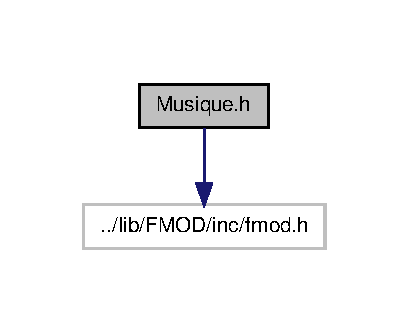
\includegraphics[width=176pt]{_musique_8h__incl}
\end{center}
\end{figure}
Ce graphe montre quels fichiers incluent directement ou indirectement ce fichier \-:\nopagebreak
\begin{figure}[H]
\begin{center}
\leavevmode
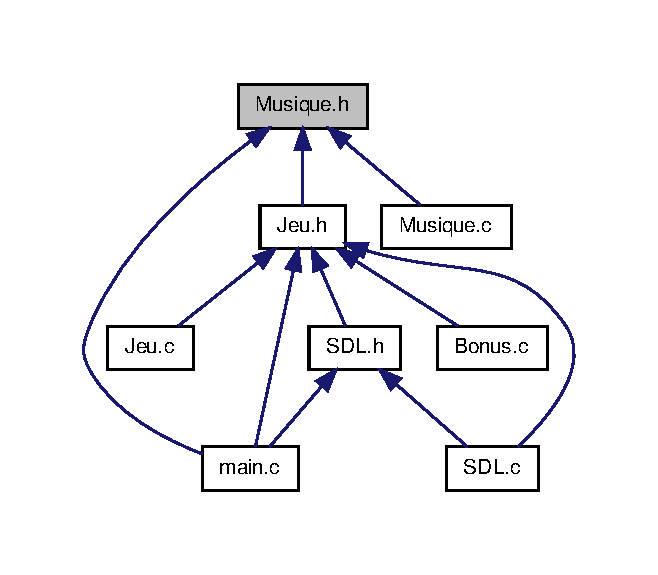
\includegraphics[width=224pt]{_musique_8h__dep__incl}
\end{center}
\end{figure}
\subsection*{Structures de données}
\begin{DoxyCompactItemize}
\item 
struct \hyperlink{struct_musique}{Musique}
\end{DoxyCompactItemize}
\subsection*{Macros}
\begin{DoxyCompactItemize}
\item 
\#define \hyperlink{_musique_8h_abcf2e20896fd8bfc6aa91cc598e6e218}{\-\_\-\-Nombre\-\_\-\-De\-\_\-\-Musique}~3
\item 
\#define \hyperlink{_musique_8h_a1429fefb7a789f6c6ef1fe2a4fa26fde}{\-\_\-\-Nombre\-\_\-\-De\-\_\-\-Bruitages}~2
\end{DoxyCompactItemize}
\subsection*{Fonctions}
\begin{DoxyCompactItemize}
\item 
F\-M\-O\-D\-\_\-\-S\-Y\-S\-T\-E\-M $\ast$ \hyperlink{_musique_8h_a6eaeb9c1618c807754684d59992d6507}{Musique\-Get\-Base\-Du\-Son} (\hyperlink{struct_musique}{Musique} $\ast$musique)
\item 
F\-M\-O\-D\-\_\-\-S\-O\-U\-N\-D $\ast$ \hyperlink{_musique_8h_af2564aa22a9d674e780a820a9cf2b328}{Musique\-Get\-Ieme\-Son\-Court} (\hyperlink{struct_musique}{Musique} $\ast$musique, int i)
\item 
F\-M\-O\-D\-\_\-\-S\-O\-U\-N\-D $\ast$ \hyperlink{_musique_8h_ada630365fea1e238fbf95631dd56ee49}{Musique\-Get\-Ieme\-Musique\-Du\-Jeu} (\hyperlink{struct_musique}{Musique} $\ast$musique, int i)
\item 
void \hyperlink{_musique_8h_a992e9a70c659319a675744a0bca3799d}{Musique\-Set\-Base\-Du\-Son} (\hyperlink{struct_musique}{Musique} $\ast$musique, F\-M\-O\-D\-\_\-\-S\-Y\-S\-T\-E\-M $\ast$base\-Du\-Son)
\item 
void \hyperlink{_musique_8h_a8126a2d49c47a2dd7ad8c484d01013ad}{Musique\-Set\-Ieme\-Son\-Court} (\hyperlink{struct_musique}{Musique} $\ast$musique, F\-M\-O\-D\-\_\-\-S\-O\-U\-N\-D $\ast$un\-Son, int i)
\item 
void \hyperlink{_musique_8h_a046f5f78ceaa10d2f8337c53ce976b22}{Musique\-Set\-Ieme\-Musique\-Du\-Jeu} (\hyperlink{struct_musique}{Musique} $\ast$musique, F\-M\-O\-D\-\_\-\-S\-O\-U\-N\-D $\ast$un\-Son, int i)
\item 
void \hyperlink{_musique_8h_adf596c7e8e14980256f0fc5c4cd23a73}{Musique\-Set\-Son\-Court} (\hyperlink{struct_musique}{Musique} $\ast$musique, F\-M\-O\-D\-\_\-\-S\-O\-U\-N\-D $\ast$$\ast$Son\-Court)
\item 
void \hyperlink{_musique_8h_aeec5162b4d8bc7da44ce55cfc364015e}{Musique\-Set\-Musique\-Du\-Jeu} (\hyperlink{struct_musique}{Musique} $\ast$musique, F\-M\-O\-D\-\_\-\-S\-O\-U\-N\-D $\ast$$\ast$musique\-Du\-Jeu)
\item 
void \hyperlink{_musique_8h_a43c750ce46e1cebd1d15d08216546b41}{Musique\-Constructeur} (\hyperlink{struct_musique}{Musique} $\ast$musique)
\item 
void \hyperlink{_musique_8h_a968015ab08fbe91eb20129567bb467bc}{Musique\-Destructeur} (\hyperlink{struct_musique}{Musique} $\ast$musique)
\item 
void \hyperlink{_musique_8h_a4ccf3ce1bf3c2fb7ee0ed6352e24fdf4}{Jouer\-Ieme\-Son\-Court} (\hyperlink{struct_musique}{Musique} $\ast$musique, int i)
\item 
void \hyperlink{_musique_8h_a83de1e788ada978f55d7d8442a3beaa8}{Jouer\-Ieme\-Musique} (\hyperlink{struct_musique}{Musique} $\ast$musique, int i, int repetition)
\item 
void \hyperlink{_musique_8h_a2f553e49e6ce20ecc91bc9b5500b0c78}{Musique\-Test\-Regression} ()
\end{DoxyCompactItemize}


\subsection{Description détaillée}
\mbox{]} Module des Musiques du jeu \begin{DoxyAuthor}{Auteur}
\{Antoine.\-C,Matthieu.\-B\} 
\end{DoxyAuthor}
\begin{DoxyVersion}{Version}
1.\-4 
\end{DoxyVersion}
\begin{DoxyDate}{Date}
19 avril 2013 
\end{DoxyDate}


Définition dans le fichier \hyperlink{_musique_8h_source}{Musique.\-h}.



\subsection{Documentation des macros}
\hypertarget{_musique_8h_a1429fefb7a789f6c6ef1fe2a4fa26fde}{\index{Musique.\-h@{Musique.\-h}!\-\_\-\-Nombre\-\_\-\-De\-\_\-\-Bruitages@{\-\_\-\-Nombre\-\_\-\-De\-\_\-\-Bruitages}}
\index{\-\_\-\-Nombre\-\_\-\-De\-\_\-\-Bruitages@{\-\_\-\-Nombre\-\_\-\-De\-\_\-\-Bruitages}!Musique.h@{Musique.\-h}}
\subsubsection[{\-\_\-\-Nombre\-\_\-\-De\-\_\-\-Bruitages}]{\setlength{\rightskip}{0pt plus 5cm}\#define \-\_\-\-Nombre\-\_\-\-De\-\_\-\-Bruitages~2}}\label{_musique_8h_a1429fefb7a789f6c6ef1fe2a4fa26fde}


Définition à la ligne 13 du fichier Musique.\-h.

\hypertarget{_musique_8h_abcf2e20896fd8bfc6aa91cc598e6e218}{\index{Musique.\-h@{Musique.\-h}!\-\_\-\-Nombre\-\_\-\-De\-\_\-\-Musique@{\-\_\-\-Nombre\-\_\-\-De\-\_\-\-Musique}}
\index{\-\_\-\-Nombre\-\_\-\-De\-\_\-\-Musique@{\-\_\-\-Nombre\-\_\-\-De\-\_\-\-Musique}!Musique.h@{Musique.\-h}}
\subsubsection[{\-\_\-\-Nombre\-\_\-\-De\-\_\-\-Musique}]{\setlength{\rightskip}{0pt plus 5cm}\#define \-\_\-\-Nombre\-\_\-\-De\-\_\-\-Musique~3}}\label{_musique_8h_abcf2e20896fd8bfc6aa91cc598e6e218}


Définition à la ligne 12 du fichier Musique.\-h.



\subsection{Documentation des fonctions}
\hypertarget{_musique_8h_a83de1e788ada978f55d7d8442a3beaa8}{\index{Musique.\-h@{Musique.\-h}!Jouer\-Ieme\-Musique@{Jouer\-Ieme\-Musique}}
\index{Jouer\-Ieme\-Musique@{Jouer\-Ieme\-Musique}!Musique.h@{Musique.\-h}}
\subsubsection[{Jouer\-Ieme\-Musique}]{\setlength{\rightskip}{0pt plus 5cm}void Jouer\-Ieme\-Musique (
\begin{DoxyParamCaption}
\item[{{\bf Musique} $\ast$}]{musique, }
\item[{int}]{i, }
\item[{int}]{repetition}
\end{DoxyParamCaption}
)}}\label{_musique_8h_a83de1e788ada978f55d7d8442a3beaa8}


Définition à la ligne 84 du fichier Musique.\-c.

\hypertarget{_musique_8h_a4ccf3ce1bf3c2fb7ee0ed6352e24fdf4}{\index{Musique.\-h@{Musique.\-h}!Jouer\-Ieme\-Son\-Court@{Jouer\-Ieme\-Son\-Court}}
\index{Jouer\-Ieme\-Son\-Court@{Jouer\-Ieme\-Son\-Court}!Musique.h@{Musique.\-h}}
\subsubsection[{Jouer\-Ieme\-Son\-Court}]{\setlength{\rightskip}{0pt plus 5cm}void Jouer\-Ieme\-Son\-Court (
\begin{DoxyParamCaption}
\item[{{\bf Musique} $\ast$}]{musique, }
\item[{int}]{i}
\end{DoxyParamCaption}
)}}\label{_musique_8h_a4ccf3ce1bf3c2fb7ee0ed6352e24fdf4}


Définition à la ligne 81 du fichier Musique.\-c.

\hypertarget{_musique_8h_a43c750ce46e1cebd1d15d08216546b41}{\index{Musique.\-h@{Musique.\-h}!Musique\-Constructeur@{Musique\-Constructeur}}
\index{Musique\-Constructeur@{Musique\-Constructeur}!Musique.h@{Musique.\-h}}
\subsubsection[{Musique\-Constructeur}]{\setlength{\rightskip}{0pt plus 5cm}void Musique\-Constructeur (
\begin{DoxyParamCaption}
\item[{{\bf Musique} $\ast$}]{musique}
\end{DoxyParamCaption}
)}}\label{_musique_8h_a43c750ce46e1cebd1d15d08216546b41}


Définition à la ligne 44 du fichier Musique.\-c.

\hypertarget{_musique_8h_a968015ab08fbe91eb20129567bb467bc}{\index{Musique.\-h@{Musique.\-h}!Musique\-Destructeur@{Musique\-Destructeur}}
\index{Musique\-Destructeur@{Musique\-Destructeur}!Musique.h@{Musique.\-h}}
\subsubsection[{Musique\-Destructeur}]{\setlength{\rightskip}{0pt plus 5cm}void Musique\-Destructeur (
\begin{DoxyParamCaption}
\item[{{\bf Musique} $\ast$}]{musique}
\end{DoxyParamCaption}
)}}\label{_musique_8h_a968015ab08fbe91eb20129567bb467bc}


Définition à la ligne 67 du fichier Musique.\-c.

\hypertarget{_musique_8h_a6eaeb9c1618c807754684d59992d6507}{\index{Musique.\-h@{Musique.\-h}!Musique\-Get\-Base\-Du\-Son@{Musique\-Get\-Base\-Du\-Son}}
\index{Musique\-Get\-Base\-Du\-Son@{Musique\-Get\-Base\-Du\-Son}!Musique.h@{Musique.\-h}}
\subsubsection[{Musique\-Get\-Base\-Du\-Son}]{\setlength{\rightskip}{0pt plus 5cm}F\-M\-O\-D\-\_\-\-S\-Y\-S\-T\-E\-M$\ast$ Musique\-Get\-Base\-Du\-Son (
\begin{DoxyParamCaption}
\item[{{\bf Musique} $\ast$}]{musique}
\end{DoxyParamCaption}
)}}\label{_musique_8h_a6eaeb9c1618c807754684d59992d6507}


Définition à la ligne 16 du fichier Musique.\-c.

\hypertarget{_musique_8h_ada630365fea1e238fbf95631dd56ee49}{\index{Musique.\-h@{Musique.\-h}!Musique\-Get\-Ieme\-Musique\-Du\-Jeu@{Musique\-Get\-Ieme\-Musique\-Du\-Jeu}}
\index{Musique\-Get\-Ieme\-Musique\-Du\-Jeu@{Musique\-Get\-Ieme\-Musique\-Du\-Jeu}!Musique.h@{Musique.\-h}}
\subsubsection[{Musique\-Get\-Ieme\-Musique\-Du\-Jeu}]{\setlength{\rightskip}{0pt plus 5cm}F\-M\-O\-D\-\_\-\-S\-O\-U\-N\-D$\ast$ Musique\-Get\-Ieme\-Musique\-Du\-Jeu (
\begin{DoxyParamCaption}
\item[{{\bf Musique} $\ast$}]{musique, }
\item[{int}]{i}
\end{DoxyParamCaption}
)}}\label{_musique_8h_ada630365fea1e238fbf95631dd56ee49}


Définition à la ligne 22 du fichier Musique.\-c.

\hypertarget{_musique_8h_af2564aa22a9d674e780a820a9cf2b328}{\index{Musique.\-h@{Musique.\-h}!Musique\-Get\-Ieme\-Son\-Court@{Musique\-Get\-Ieme\-Son\-Court}}
\index{Musique\-Get\-Ieme\-Son\-Court@{Musique\-Get\-Ieme\-Son\-Court}!Musique.h@{Musique.\-h}}
\subsubsection[{Musique\-Get\-Ieme\-Son\-Court}]{\setlength{\rightskip}{0pt plus 5cm}F\-M\-O\-D\-\_\-\-S\-O\-U\-N\-D$\ast$ Musique\-Get\-Ieme\-Son\-Court (
\begin{DoxyParamCaption}
\item[{{\bf Musique} $\ast$}]{musique, }
\item[{int}]{i}
\end{DoxyParamCaption}
)}}\label{_musique_8h_af2564aa22a9d674e780a820a9cf2b328}


Définition à la ligne 19 du fichier Musique.\-c.

\hypertarget{_musique_8h_a992e9a70c659319a675744a0bca3799d}{\index{Musique.\-h@{Musique.\-h}!Musique\-Set\-Base\-Du\-Son@{Musique\-Set\-Base\-Du\-Son}}
\index{Musique\-Set\-Base\-Du\-Son@{Musique\-Set\-Base\-Du\-Son}!Musique.h@{Musique.\-h}}
\subsubsection[{Musique\-Set\-Base\-Du\-Son}]{\setlength{\rightskip}{0pt plus 5cm}void Musique\-Set\-Base\-Du\-Son (
\begin{DoxyParamCaption}
\item[{{\bf Musique} $\ast$}]{musique, }
\item[{F\-M\-O\-D\-\_\-\-S\-Y\-S\-T\-E\-M $\ast$}]{base\-Du\-Son}
\end{DoxyParamCaption}
)}}\label{_musique_8h_a992e9a70c659319a675744a0bca3799d}


Définition à la ligne 27 du fichier Musique.\-c.

\hypertarget{_musique_8h_a046f5f78ceaa10d2f8337c53ce976b22}{\index{Musique.\-h@{Musique.\-h}!Musique\-Set\-Ieme\-Musique\-Du\-Jeu@{Musique\-Set\-Ieme\-Musique\-Du\-Jeu}}
\index{Musique\-Set\-Ieme\-Musique\-Du\-Jeu@{Musique\-Set\-Ieme\-Musique\-Du\-Jeu}!Musique.h@{Musique.\-h}}
\subsubsection[{Musique\-Set\-Ieme\-Musique\-Du\-Jeu}]{\setlength{\rightskip}{0pt plus 5cm}void Musique\-Set\-Ieme\-Musique\-Du\-Jeu (
\begin{DoxyParamCaption}
\item[{{\bf Musique} $\ast$}]{musique, }
\item[{F\-M\-O\-D\-\_\-\-S\-O\-U\-N\-D $\ast$}]{un\-Son, }
\item[{int}]{i}
\end{DoxyParamCaption}
)}}\label{_musique_8h_a046f5f78ceaa10d2f8337c53ce976b22}


Définition à la ligne 36 du fichier Musique.\-c.

\hypertarget{_musique_8h_a8126a2d49c47a2dd7ad8c484d01013ad}{\index{Musique.\-h@{Musique.\-h}!Musique\-Set\-Ieme\-Son\-Court@{Musique\-Set\-Ieme\-Son\-Court}}
\index{Musique\-Set\-Ieme\-Son\-Court@{Musique\-Set\-Ieme\-Son\-Court}!Musique.h@{Musique.\-h}}
\subsubsection[{Musique\-Set\-Ieme\-Son\-Court}]{\setlength{\rightskip}{0pt plus 5cm}void Musique\-Set\-Ieme\-Son\-Court (
\begin{DoxyParamCaption}
\item[{{\bf Musique} $\ast$}]{musique, }
\item[{F\-M\-O\-D\-\_\-\-S\-O\-U\-N\-D $\ast$}]{un\-Son, }
\item[{int}]{i}
\end{DoxyParamCaption}
)}}\label{_musique_8h_a8126a2d49c47a2dd7ad8c484d01013ad}


Définition à la ligne 30 du fichier Musique.\-c.

\hypertarget{_musique_8h_aeec5162b4d8bc7da44ce55cfc364015e}{\index{Musique.\-h@{Musique.\-h}!Musique\-Set\-Musique\-Du\-Jeu@{Musique\-Set\-Musique\-Du\-Jeu}}
\index{Musique\-Set\-Musique\-Du\-Jeu@{Musique\-Set\-Musique\-Du\-Jeu}!Musique.h@{Musique.\-h}}
\subsubsection[{Musique\-Set\-Musique\-Du\-Jeu}]{\setlength{\rightskip}{0pt plus 5cm}void Musique\-Set\-Musique\-Du\-Jeu (
\begin{DoxyParamCaption}
\item[{{\bf Musique} $\ast$}]{musique, }
\item[{F\-M\-O\-D\-\_\-\-S\-O\-U\-N\-D $\ast$$\ast$}]{musique\-Du\-Jeu}
\end{DoxyParamCaption}
)}}\label{_musique_8h_aeec5162b4d8bc7da44ce55cfc364015e}


Définition à la ligne 39 du fichier Musique.\-c.

\hypertarget{_musique_8h_adf596c7e8e14980256f0fc5c4cd23a73}{\index{Musique.\-h@{Musique.\-h}!Musique\-Set\-Son\-Court@{Musique\-Set\-Son\-Court}}
\index{Musique\-Set\-Son\-Court@{Musique\-Set\-Son\-Court}!Musique.h@{Musique.\-h}}
\subsubsection[{Musique\-Set\-Son\-Court}]{\setlength{\rightskip}{0pt plus 5cm}void Musique\-Set\-Son\-Court (
\begin{DoxyParamCaption}
\item[{{\bf Musique} $\ast$}]{musique, }
\item[{F\-M\-O\-D\-\_\-\-S\-O\-U\-N\-D $\ast$$\ast$}]{Son\-Court}
\end{DoxyParamCaption}
)}}\label{_musique_8h_adf596c7e8e14980256f0fc5c4cd23a73}


Définition à la ligne 33 du fichier Musique.\-c.

\hypertarget{_musique_8h_a2f553e49e6ce20ecc91bc9b5500b0c78}{\index{Musique.\-h@{Musique.\-h}!Musique\-Test\-Regression@{Musique\-Test\-Regression}}
\index{Musique\-Test\-Regression@{Musique\-Test\-Regression}!Musique.h@{Musique.\-h}}
\subsubsection[{Musique\-Test\-Regression}]{\setlength{\rightskip}{0pt plus 5cm}void Musique\-Test\-Regression (
\begin{DoxyParamCaption}
{}
\end{DoxyParamCaption}
)}}\label{_musique_8h_a2f553e49e6ce20ecc91bc9b5500b0c78}
fonction qui teste le Module 

Définition à la ligne 90 du fichier Musique.\-c.


\hypertarget{_s_d_l_8c}{\section{Référence du fichier S\-D\-L.\-c}
\label{_s_d_l_8c}\index{S\-D\-L.\-c@{S\-D\-L.\-c}}
}
{\ttfamily \#include \char`\"{}Jeu.\-h\char`\"{}}\\*
{\ttfamily \#include \char`\"{}S\-D\-L.\-h\char`\"{}}\\*
{\ttfamily \#include $<$assert.\-h$>$}\\*
{\ttfamily \#include $<$S\-D\-L/\-S\-D\-L.\-h$>$}\\*
{\ttfamily \#include $<$time.\-h$>$}\\*
{\ttfamily \#include \char`\"{}Joystick.\-h\char`\"{}}\\*
{\ttfamily \#include $<$S\-D\-L/\-S\-D\-L\-\_\-ttf.\-h$>$}\\*
{\ttfamily \#include $<$string.\-h$>$}\\*
Graphe des dépendances par inclusion de S\-D\-L.\-c\-:\nopagebreak
\begin{figure}[H]
\begin{center}
\leavevmode
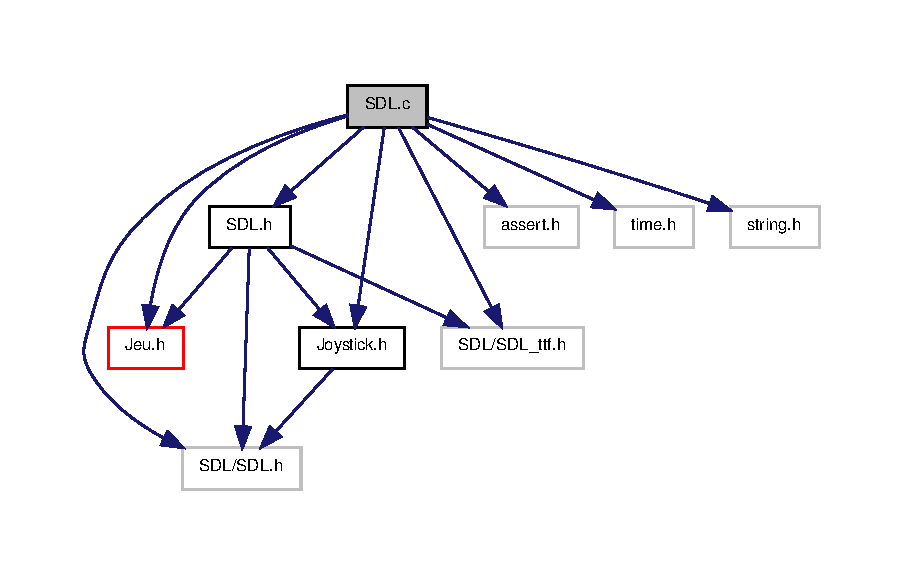
\includegraphics[width=350pt]{_s_d_l_8c__incl}
\end{center}
\end{figure}
\subsection*{Fonctions}
\begin{DoxyCompactItemize}
\item 
\hyperlink{struct_jeu}{Jeu} $\ast$ \hyperlink{_s_d_l_8c_aa7223cb3ce4fe6f4c83d6a01adc66cbd}{S\-D\-L\-Get\-Jeu} (\hyperlink{struct_s_d_l}{S\-D\-L} $\ast$sdl)
\item 
S\-D\-L\-\_\-\-Surface $\ast$ \hyperlink{_s_d_l_8c_acca01b95fb78179e3051d8d411b8a9cd}{S\-D\-L\-Get\-Ieme\-Texture} (const \hyperlink{struct_s_d_l}{S\-D\-L} $\ast$sdl, unsigned int i)
\item 
\hyperlink{struct_manette}{Manette} $\ast$ \hyperlink{_s_d_l_8c_a0739253f7d24014416204f6d64c565b6}{S\-D\-L\-Get\-Ieme\-Manette} (const \hyperlink{struct_s_d_l}{S\-D\-L} $\ast$sdl, unsigned int i)
\item 
S\-D\-L\-\_\-\-Surface $\ast$ \hyperlink{_s_d_l_8c_a7596bb1c6890b99a64e59f6b732a2fe1}{S\-D\-L\-Get\-Textures} (const \hyperlink{struct_s_d_l}{S\-D\-L} $\ast$sdl)
\item 
void \hyperlink{_s_d_l_8c_a29faea1dc4bb87f4538e14d944b55a5e}{S\-D\-L\-Set\-Jeu} (\hyperlink{struct_s_d_l}{S\-D\-L} $\ast$sdl, \hyperlink{struct_jeu}{Jeu} $\ast$jeu)
\item 
void \hyperlink{_s_d_l_8c_ad7897b59aff5363840beb85766e25e47}{S\-D\-L\-Set\-Ieme\-Texture} (\hyperlink{struct_s_d_l}{S\-D\-L} $\ast$sdl, unsigned int i, S\-D\-L\-\_\-\-Surface $\ast$texture)
\item 
S\-D\-L\-\_\-\-Surface $\ast$ \hyperlink{_s_d_l_8c_a36684beb5e5ec3f9397a2976415141b7}{S\-D\-L\-Charge\-Image} (const char $\ast$nomfichier)
\item 
void \hyperlink{_s_d_l_8c_a99f60fc0c0adee46a2703d3829ecb472}{S\-D\-L\-Applique\-Surface} (S\-D\-L\-\_\-\-Surface $\ast$surface\-A, S\-D\-L\-\_\-\-Surface $\ast$surface\-B, const int position\-X, const int position\-Y)
\item 
void \hyperlink{_s_d_l_8c_a2a26b97bd3b8195da9e8ac79bad18896}{S\-D\-L\-Constructeur} (\hyperlink{struct_s_d_l}{S\-D\-L} $\ast$sdl, S\-D\-L\-\_\-\-Surface $\ast$ecran, \hyperlink{struct_jeu}{Jeu} $\ast$jeu, \hyperlink{struct_manette}{Manette} $\ast$manettes)
\item 
void \hyperlink{_s_d_l_8c_a18f1617d8034417cd2f06cc9c4dbedf2}{S\-D\-L\-Destructeur} (\hyperlink{struct_s_d_l}{S\-D\-L} $\ast$sdl)
\item 
void \hyperlink{_s_d_l_8c_a7167f5c196fc5e167bfabde1a730e81d}{pause} ()
\item 
void \hyperlink{_s_d_l_8c_acee5e34159940dd36ec30124193530df}{S\-D\-L\-Intro} (short int $\ast$jeu\-Re\-Init, S\-D\-L\-\_\-\-Surface $\ast$ecran)
\item 
void \hyperlink{_s_d_l_8c_aa01afa367fb926561efefd9ee28941c5}{S\-D\-L\-Jeu\-Init\-N} (\hyperlink{struct_s_d_l}{S\-D\-L} $\ast$sdl, int $\ast$scores, S\-D\-L\-\_\-\-Surface $\ast$ecran)
\item 
void \hyperlink{_s_d_l_8c_ae4216fdeea2ef708146cfba234e0a0ff}{S\-D\-L\-Boucle\-Jeu} (\hyperlink{struct_s_d_l}{S\-D\-L} $\ast$sdl, short int $\ast$jeu\-Re\-Init)
\item 
void \hyperlink{_s_d_l_8c_a5307e0546a65557e28218096444fe16e}{S\-D\-L\-Action\-Manette} (\hyperlink{struct_joueur}{Joueur} $\ast$joueur, \hyperlink{_moto_8h_a224b9163917ac32fc95a60d8c1eec3aa}{Direction} direction, \hyperlink{struct_grid}{Grid} $\ast$grille)
\item 
void \hyperlink{_s_d_l_8c_a0a164a520a75c594cf10cd3cfdca3814}{S\-D\-L\-Affiche\-Motos} (\hyperlink{struct_s_d_l}{S\-D\-L} $\ast$sdl)
\item 
void \hyperlink{_s_d_l_8c_a511761d608b92801c934aad221f762ce}{S\-D\-L\-Affiche\-Murs} (\hyperlink{struct_s_d_l}{S\-D\-L} $\ast$sdl)
\item 
void \hyperlink{_s_d_l_8c_ac27595c16fe8fbd8ee635cb6c8d9ec40}{S\-D\-L\-Affiche\-Bonus} (\hyperlink{struct_s_d_l}{S\-D\-L} $\ast$sdl)
\item 
void \hyperlink{_s_d_l_8c_a87530d8f5fdcb529d517fb86bc927e63}{S\-D\-L\-Affiche\-Interface} (\hyperlink{struct_s_d_l}{S\-D\-L} $\ast$sdl)
\item 
void \hyperlink{_s_d_l_8c_ab2b2544e3bfaa5cce134a84429e8dbd6}{S\-D\-L\-Affiche\-Textes} (\hyperlink{struct_s_d_l}{S\-D\-L} $\ast$sdl, char $\ast$chaine\-De\-Caractere, \hyperlink{_couleur_8h_aa304d0ca681f782b1d7735da33037dd7}{Couleur} une\-Couleur)
\item 
void \hyperlink{_s_d_l_8c_a0583e9dfa2d7caa1c39a34b2adf6e9e5}{S\-D\-L\-Affiche\-Scores} (\hyperlink{struct_s_d_l}{S\-D\-L} $\ast$sdl)
\item 
void \hyperlink{_s_d_l_8c_abcc23c44c3c837b312d055a71e1c93d5}{S\-D\-L\-Affiche\-Jeu} (\hyperlink{struct_s_d_l}{S\-D\-L} $\ast$sdl)
\item 
void \hyperlink{_s_d_l_8c_a240e53a13bc5d885bfd85530fa798e4a}{S\-D\-L\-Test\-Regression} ()
\end{DoxyCompactItemize}


\subsection{Description détaillée}
\mbox{]} Module qui gère les affichage du jeu,ainsi que les manettes \begin{DoxyAuthor}{Auteur}
\{Antoine.\-C,Matthieu.\-B\} 
\end{DoxyAuthor}
\begin{DoxyVersion}{Version}
0.\-1 
\end{DoxyVersion}
\begin{DoxyDate}{Date}
19 mars 2013 
\end{DoxyDate}


Définition dans le fichier \hyperlink{_s_d_l_8c_source}{S\-D\-L.\-c}.



\subsection{Documentation des fonctions}
\hypertarget{_s_d_l_8c_a7167f5c196fc5e167bfabde1a730e81d}{\index{S\-D\-L.\-c@{S\-D\-L.\-c}!pause@{pause}}
\index{pause@{pause}!SDL.c@{S\-D\-L.\-c}}
\subsubsection[{pause}]{\setlength{\rightskip}{0pt plus 5cm}void pause (
\begin{DoxyParamCaption}
{}
\end{DoxyParamCaption}
)}}\label{_s_d_l_8c_a7167f5c196fc5e167bfabde1a730e81d}


Définition à la ligne 148 du fichier S\-D\-L.\-c.

\hypertarget{_s_d_l_8c_a5307e0546a65557e28218096444fe16e}{\index{S\-D\-L.\-c@{S\-D\-L.\-c}!S\-D\-L\-Action\-Manette@{S\-D\-L\-Action\-Manette}}
\index{S\-D\-L\-Action\-Manette@{S\-D\-L\-Action\-Manette}!SDL.c@{S\-D\-L.\-c}}
\subsubsection[{S\-D\-L\-Action\-Manette}]{\setlength{\rightskip}{0pt plus 5cm}void S\-D\-L\-Action\-Manette (
\begin{DoxyParamCaption}
\item[{{\bf Joueur} $\ast$}]{joueur, }
\item[{{\bf Direction}}]{direction, }
\item[{{\bf Grid} $\ast$}]{grille}
\end{DoxyParamCaption}
)}}\label{_s_d_l_8c_a5307e0546a65557e28218096444fe16e}


Définition à la ligne 584 du fichier S\-D\-L.\-c.

\hypertarget{_s_d_l_8c_ac27595c16fe8fbd8ee635cb6c8d9ec40}{\index{S\-D\-L.\-c@{S\-D\-L.\-c}!S\-D\-L\-Affiche\-Bonus@{S\-D\-L\-Affiche\-Bonus}}
\index{S\-D\-L\-Affiche\-Bonus@{S\-D\-L\-Affiche\-Bonus}!SDL.c@{S\-D\-L.\-c}}
\subsubsection[{S\-D\-L\-Affiche\-Bonus}]{\setlength{\rightskip}{0pt plus 5cm}void S\-D\-L\-Affiche\-Bonus (
\begin{DoxyParamCaption}
\item[{{\bf S\-D\-L} $\ast$}]{sdl}
\end{DoxyParamCaption}
)}}\label{_s_d_l_8c_ac27595c16fe8fbd8ee635cb6c8d9ec40}


Définition à la ligne 721 du fichier S\-D\-L.\-c.

\hypertarget{_s_d_l_8c_a87530d8f5fdcb529d517fb86bc927e63}{\index{S\-D\-L.\-c@{S\-D\-L.\-c}!S\-D\-L\-Affiche\-Interface@{S\-D\-L\-Affiche\-Interface}}
\index{S\-D\-L\-Affiche\-Interface@{S\-D\-L\-Affiche\-Interface}!SDL.c@{S\-D\-L.\-c}}
\subsubsection[{S\-D\-L\-Affiche\-Interface}]{\setlength{\rightskip}{0pt plus 5cm}void S\-D\-L\-Affiche\-Interface (
\begin{DoxyParamCaption}
\item[{{\bf S\-D\-L} $\ast$}]{sdl}
\end{DoxyParamCaption}
)}}\label{_s_d_l_8c_a87530d8f5fdcb529d517fb86bc927e63}


Définition à la ligne 741 du fichier S\-D\-L.\-c.

\hypertarget{_s_d_l_8c_abcc23c44c3c837b312d055a71e1c93d5}{\index{S\-D\-L.\-c@{S\-D\-L.\-c}!S\-D\-L\-Affiche\-Jeu@{S\-D\-L\-Affiche\-Jeu}}
\index{S\-D\-L\-Affiche\-Jeu@{S\-D\-L\-Affiche\-Jeu}!SDL.c@{S\-D\-L.\-c}}
\subsubsection[{S\-D\-L\-Affiche\-Jeu}]{\setlength{\rightskip}{0pt plus 5cm}void S\-D\-L\-Affiche\-Jeu (
\begin{DoxyParamCaption}
\item[{{\bf S\-D\-L} $\ast$}]{sdl}
\end{DoxyParamCaption}
)}}\label{_s_d_l_8c_abcc23c44c3c837b312d055a71e1c93d5}


Définition à la ligne 888 du fichier S\-D\-L.\-c.

\hypertarget{_s_d_l_8c_a0a164a520a75c594cf10cd3cfdca3814}{\index{S\-D\-L.\-c@{S\-D\-L.\-c}!S\-D\-L\-Affiche\-Motos@{S\-D\-L\-Affiche\-Motos}}
\index{S\-D\-L\-Affiche\-Motos@{S\-D\-L\-Affiche\-Motos}!SDL.c@{S\-D\-L.\-c}}
\subsubsection[{S\-D\-L\-Affiche\-Motos}]{\setlength{\rightskip}{0pt plus 5cm}void S\-D\-L\-Affiche\-Motos (
\begin{DoxyParamCaption}
\item[{{\bf S\-D\-L} $\ast$}]{sdl}
\end{DoxyParamCaption}
)}}\label{_s_d_l_8c_a0a164a520a75c594cf10cd3cfdca3814}


Définition à la ligne 660 du fichier S\-D\-L.\-c.

\hypertarget{_s_d_l_8c_a511761d608b92801c934aad221f762ce}{\index{S\-D\-L.\-c@{S\-D\-L.\-c}!S\-D\-L\-Affiche\-Murs@{S\-D\-L\-Affiche\-Murs}}
\index{S\-D\-L\-Affiche\-Murs@{S\-D\-L\-Affiche\-Murs}!SDL.c@{S\-D\-L.\-c}}
\subsubsection[{S\-D\-L\-Affiche\-Murs}]{\setlength{\rightskip}{0pt plus 5cm}void S\-D\-L\-Affiche\-Murs (
\begin{DoxyParamCaption}
\item[{{\bf S\-D\-L} $\ast$}]{sdl}
\end{DoxyParamCaption}
)}}\label{_s_d_l_8c_a511761d608b92801c934aad221f762ce}


Définition à la ligne 685 du fichier S\-D\-L.\-c.

\hypertarget{_s_d_l_8c_a0583e9dfa2d7caa1c39a34b2adf6e9e5}{\index{S\-D\-L.\-c@{S\-D\-L.\-c}!S\-D\-L\-Affiche\-Scores@{S\-D\-L\-Affiche\-Scores}}
\index{S\-D\-L\-Affiche\-Scores@{S\-D\-L\-Affiche\-Scores}!SDL.c@{S\-D\-L.\-c}}
\subsubsection[{S\-D\-L\-Affiche\-Scores}]{\setlength{\rightskip}{0pt plus 5cm}void S\-D\-L\-Affiche\-Scores (
\begin{DoxyParamCaption}
\item[{{\bf S\-D\-L} $\ast$}]{sdl}
\end{DoxyParamCaption}
)}}\label{_s_d_l_8c_a0583e9dfa2d7caa1c39a34b2adf6e9e5}
$<$affichage de la ligne supérieure

$<$affichage de la ligne inférieure 

Définition à la ligne 834 du fichier S\-D\-L.\-c.

\hypertarget{_s_d_l_8c_ab2b2544e3bfaa5cce134a84429e8dbd6}{\index{S\-D\-L.\-c@{S\-D\-L.\-c}!S\-D\-L\-Affiche\-Textes@{S\-D\-L\-Affiche\-Textes}}
\index{S\-D\-L\-Affiche\-Textes@{S\-D\-L\-Affiche\-Textes}!SDL.c@{S\-D\-L.\-c}}
\subsubsection[{S\-D\-L\-Affiche\-Textes}]{\setlength{\rightskip}{0pt plus 5cm}void S\-D\-L\-Affiche\-Textes (
\begin{DoxyParamCaption}
\item[{{\bf S\-D\-L} $\ast$}]{sdl, }
\item[{char $\ast$}]{chaine\-De\-Caractere, }
\item[{{\bf Couleur}}]{une\-Couleur}
\end{DoxyParamCaption}
)}}\label{_s_d_l_8c_ab2b2544e3bfaa5cce134a84429e8dbd6}


Définition à la ligne 761 du fichier S\-D\-L.\-c.

\hypertarget{_s_d_l_8c_a99f60fc0c0adee46a2703d3829ecb472}{\index{S\-D\-L.\-c@{S\-D\-L.\-c}!S\-D\-L\-Applique\-Surface@{S\-D\-L\-Applique\-Surface}}
\index{S\-D\-L\-Applique\-Surface@{S\-D\-L\-Applique\-Surface}!SDL.c@{S\-D\-L.\-c}}
\subsubsection[{S\-D\-L\-Applique\-Surface}]{\setlength{\rightskip}{0pt plus 5cm}void S\-D\-L\-Applique\-Surface (
\begin{DoxyParamCaption}
\item[{S\-D\-L\-\_\-\-Surface $\ast$}]{surface\-A, }
\item[{S\-D\-L\-\_\-\-Surface $\ast$}]{surface\-B, }
\item[{const int}]{position\-X, }
\item[{const int}]{position\-Y}
\end{DoxyParamCaption}
)}}\label{_s_d_l_8c_a99f60fc0c0adee46a2703d3829ecb472}
!$<$ Make a temporary rectangle to hold the offsets

!$<$ Give the offsets to the rectangle

!$<$ Blit the surface 

Définition à la ligne 56 du fichier S\-D\-L.\-c.

\hypertarget{_s_d_l_8c_ae4216fdeea2ef708146cfba234e0a0ff}{\index{S\-D\-L.\-c@{S\-D\-L.\-c}!S\-D\-L\-Boucle\-Jeu@{S\-D\-L\-Boucle\-Jeu}}
\index{S\-D\-L\-Boucle\-Jeu@{S\-D\-L\-Boucle\-Jeu}!SDL.c@{S\-D\-L.\-c}}
\subsubsection[{S\-D\-L\-Boucle\-Jeu}]{\setlength{\rightskip}{0pt plus 5cm}void S\-D\-L\-Boucle\-Jeu (
\begin{DoxyParamCaption}
\item[{{\bf S\-D\-L} $\ast$}]{sdl, }
\item[{short int $\ast$}]{jeu\-Re\-Init}
\end{DoxyParamCaption}
)}}\label{_s_d_l_8c_ae4216fdeea2ef708146cfba234e0a0ff}
!$<$Si le jeu a renvoyé un nouveau commentaire 

Définition à la ligne 406 du fichier S\-D\-L.\-c.

\hypertarget{_s_d_l_8c_a36684beb5e5ec3f9397a2976415141b7}{\index{S\-D\-L.\-c@{S\-D\-L.\-c}!S\-D\-L\-Charge\-Image@{S\-D\-L\-Charge\-Image}}
\index{S\-D\-L\-Charge\-Image@{S\-D\-L\-Charge\-Image}!SDL.c@{S\-D\-L.\-c}}
\subsubsection[{S\-D\-L\-Charge\-Image}]{\setlength{\rightskip}{0pt plus 5cm}S\-D\-L\-\_\-\-Surface$\ast$ S\-D\-L\-Charge\-Image (
\begin{DoxyParamCaption}
\item[{const char $\ast$}]{nomfichier}
\end{DoxyParamCaption}
)}}\label{_s_d_l_8c_a36684beb5e5ec3f9397a2976415141b7}
!$<$ Temporary storage for the image that's loaded

!$<$ Load the image

!$<$ If nothing went wrong in loading the image

!$<$ Return the optimized image 

Définition à la ligne 41 du fichier S\-D\-L.\-c.

\hypertarget{_s_d_l_8c_a2a26b97bd3b8195da9e8ac79bad18896}{\index{S\-D\-L.\-c@{S\-D\-L.\-c}!S\-D\-L\-Constructeur@{S\-D\-L\-Constructeur}}
\index{S\-D\-L\-Constructeur@{S\-D\-L\-Constructeur}!SDL.c@{S\-D\-L.\-c}}
\subsubsection[{S\-D\-L\-Constructeur}]{\setlength{\rightskip}{0pt plus 5cm}void S\-D\-L\-Constructeur (
\begin{DoxyParamCaption}
\item[{{\bf S\-D\-L} $\ast$}]{sdl, }
\item[{S\-D\-L\-\_\-\-Surface $\ast$}]{ecran, }
\item[{{\bf Jeu} $\ast$}]{jeu, }
\item[{{\bf Manette} $\ast$}]{manettes}
\end{DoxyParamCaption}
)}}\label{_s_d_l_8c_a2a26b97bd3b8195da9e8ac79bad18896}


Définition à la ligne 70 du fichier S\-D\-L.\-c.

\hypertarget{_s_d_l_8c_a18f1617d8034417cd2f06cc9c4dbedf2}{\index{S\-D\-L.\-c@{S\-D\-L.\-c}!S\-D\-L\-Destructeur@{S\-D\-L\-Destructeur}}
\index{S\-D\-L\-Destructeur@{S\-D\-L\-Destructeur}!SDL.c@{S\-D\-L.\-c}}
\subsubsection[{S\-D\-L\-Destructeur}]{\setlength{\rightskip}{0pt plus 5cm}void S\-D\-L\-Destructeur (
\begin{DoxyParamCaption}
\item[{{\bf S\-D\-L} $\ast$}]{sdl}
\end{DoxyParamCaption}
)}}\label{_s_d_l_8c_a18f1617d8034417cd2f06cc9c4dbedf2}


Définition à la ligne 132 du fichier S\-D\-L.\-c.

\hypertarget{_s_d_l_8c_a0739253f7d24014416204f6d64c565b6}{\index{S\-D\-L.\-c@{S\-D\-L.\-c}!S\-D\-L\-Get\-Ieme\-Manette@{S\-D\-L\-Get\-Ieme\-Manette}}
\index{S\-D\-L\-Get\-Ieme\-Manette@{S\-D\-L\-Get\-Ieme\-Manette}!SDL.c@{S\-D\-L.\-c}}
\subsubsection[{S\-D\-L\-Get\-Ieme\-Manette}]{\setlength{\rightskip}{0pt plus 5cm}{\bf Manette}$\ast$ S\-D\-L\-Get\-Ieme\-Manette (
\begin{DoxyParamCaption}
\item[{const {\bf S\-D\-L} $\ast$}]{sdl, }
\item[{unsigned int}]{i}
\end{DoxyParamCaption}
)}}\label{_s_d_l_8c_a0739253f7d24014416204f6d64c565b6}


Définition à la ligne 24 du fichier S\-D\-L.\-c.

\hypertarget{_s_d_l_8c_acca01b95fb78179e3051d8d411b8a9cd}{\index{S\-D\-L.\-c@{S\-D\-L.\-c}!S\-D\-L\-Get\-Ieme\-Texture@{S\-D\-L\-Get\-Ieme\-Texture}}
\index{S\-D\-L\-Get\-Ieme\-Texture@{S\-D\-L\-Get\-Ieme\-Texture}!SDL.c@{S\-D\-L.\-c}}
\subsubsection[{S\-D\-L\-Get\-Ieme\-Texture}]{\setlength{\rightskip}{0pt plus 5cm}S\-D\-L\-\_\-\-Surface$\ast$ S\-D\-L\-Get\-Ieme\-Texture (
\begin{DoxyParamCaption}
\item[{const {\bf S\-D\-L} $\ast$}]{sdl, }
\item[{unsigned int}]{i}
\end{DoxyParamCaption}
)}}\label{_s_d_l_8c_acca01b95fb78179e3051d8d411b8a9cd}


Définition à la ligne 21 du fichier S\-D\-L.\-c.

\hypertarget{_s_d_l_8c_aa7223cb3ce4fe6f4c83d6a01adc66cbd}{\index{S\-D\-L.\-c@{S\-D\-L.\-c}!S\-D\-L\-Get\-Jeu@{S\-D\-L\-Get\-Jeu}}
\index{S\-D\-L\-Get\-Jeu@{S\-D\-L\-Get\-Jeu}!SDL.c@{S\-D\-L.\-c}}
\subsubsection[{S\-D\-L\-Get\-Jeu}]{\setlength{\rightskip}{0pt plus 5cm}{\bf Jeu}$\ast$ S\-D\-L\-Get\-Jeu (
\begin{DoxyParamCaption}
\item[{{\bf S\-D\-L} $\ast$}]{sdl}
\end{DoxyParamCaption}
)}}\label{_s_d_l_8c_aa7223cb3ce4fe6f4c83d6a01adc66cbd}


Définition à la ligne 18 du fichier S\-D\-L.\-c.

\hypertarget{_s_d_l_8c_a7596bb1c6890b99a64e59f6b732a2fe1}{\index{S\-D\-L.\-c@{S\-D\-L.\-c}!S\-D\-L\-Get\-Textures@{S\-D\-L\-Get\-Textures}}
\index{S\-D\-L\-Get\-Textures@{S\-D\-L\-Get\-Textures}!SDL.c@{S\-D\-L.\-c}}
\subsubsection[{S\-D\-L\-Get\-Textures}]{\setlength{\rightskip}{0pt plus 5cm}S\-D\-L\-\_\-\-Surface$\ast$ S\-D\-L\-Get\-Textures (
\begin{DoxyParamCaption}
\item[{const {\bf S\-D\-L} $\ast$}]{sdl}
\end{DoxyParamCaption}
)}}\label{_s_d_l_8c_a7596bb1c6890b99a64e59f6b732a2fe1}


Définition à la ligne 27 du fichier S\-D\-L.\-c.

\hypertarget{_s_d_l_8c_acee5e34159940dd36ec30124193530df}{\index{S\-D\-L.\-c@{S\-D\-L.\-c}!S\-D\-L\-Intro@{S\-D\-L\-Intro}}
\index{S\-D\-L\-Intro@{S\-D\-L\-Intro}!SDL.c@{S\-D\-L.\-c}}
\subsubsection[{S\-D\-L\-Intro}]{\setlength{\rightskip}{0pt plus 5cm}void S\-D\-L\-Intro (
\begin{DoxyParamCaption}
\item[{short int $\ast$}]{jeu\-Re\-Init, }
\item[{S\-D\-L\-\_\-\-Surface $\ast$}]{ecran}
\end{DoxyParamCaption}
)}}\label{_s_d_l_8c_acee5e34159940dd36ec30124193530df}


Définition à la ligne 164 du fichier S\-D\-L.\-c.

\hypertarget{_s_d_l_8c_aa01afa367fb926561efefd9ee28941c5}{\index{S\-D\-L.\-c@{S\-D\-L.\-c}!S\-D\-L\-Jeu\-Init\-N@{S\-D\-L\-Jeu\-Init\-N}}
\index{S\-D\-L\-Jeu\-Init\-N@{S\-D\-L\-Jeu\-Init\-N}!SDL.c@{S\-D\-L.\-c}}
\subsubsection[{S\-D\-L\-Jeu\-Init\-N}]{\setlength{\rightskip}{0pt plus 5cm}void S\-D\-L\-Jeu\-Init\-N (
\begin{DoxyParamCaption}
\item[{{\bf S\-D\-L} $\ast$}]{sdl, }
\item[{int $\ast$}]{scores, }
\item[{S\-D\-L\-\_\-\-Surface $\ast$}]{ecran}
\end{DoxyParamCaption}
)}}\label{_s_d_l_8c_aa01afa367fb926561efefd9ee28941c5}


Définition à la ligne 183 du fichier S\-D\-L.\-c.

\hypertarget{_s_d_l_8c_ad7897b59aff5363840beb85766e25e47}{\index{S\-D\-L.\-c@{S\-D\-L.\-c}!S\-D\-L\-Set\-Ieme\-Texture@{S\-D\-L\-Set\-Ieme\-Texture}}
\index{S\-D\-L\-Set\-Ieme\-Texture@{S\-D\-L\-Set\-Ieme\-Texture}!SDL.c@{S\-D\-L.\-c}}
\subsubsection[{S\-D\-L\-Set\-Ieme\-Texture}]{\setlength{\rightskip}{0pt plus 5cm}void S\-D\-L\-Set\-Ieme\-Texture (
\begin{DoxyParamCaption}
\item[{{\bf S\-D\-L} $\ast$}]{sdl, }
\item[{unsigned int}]{i, }
\item[{S\-D\-L\-\_\-\-Surface $\ast$}]{texture}
\end{DoxyParamCaption}
)}}\label{_s_d_l_8c_ad7897b59aff5363840beb85766e25e47}


Définition à la ligne 34 du fichier S\-D\-L.\-c.

\hypertarget{_s_d_l_8c_a29faea1dc4bb87f4538e14d944b55a5e}{\index{S\-D\-L.\-c@{S\-D\-L.\-c}!S\-D\-L\-Set\-Jeu@{S\-D\-L\-Set\-Jeu}}
\index{S\-D\-L\-Set\-Jeu@{S\-D\-L\-Set\-Jeu}!SDL.c@{S\-D\-L.\-c}}
\subsubsection[{S\-D\-L\-Set\-Jeu}]{\setlength{\rightskip}{0pt plus 5cm}void S\-D\-L\-Set\-Jeu (
\begin{DoxyParamCaption}
\item[{{\bf S\-D\-L} $\ast$}]{sdl, }
\item[{{\bf Jeu} $\ast$}]{jeu}
\end{DoxyParamCaption}
)}}\label{_s_d_l_8c_a29faea1dc4bb87f4538e14d944b55a5e}


Définition à la ligne 31 du fichier S\-D\-L.\-c.

\hypertarget{_s_d_l_8c_a240e53a13bc5d885bfd85530fa798e4a}{\index{S\-D\-L.\-c@{S\-D\-L.\-c}!S\-D\-L\-Test\-Regression@{S\-D\-L\-Test\-Regression}}
\index{S\-D\-L\-Test\-Regression@{S\-D\-L\-Test\-Regression}!SDL.c@{S\-D\-L.\-c}}
\subsubsection[{S\-D\-L\-Test\-Regression}]{\setlength{\rightskip}{0pt plus 5cm}S\-D\-L\-Test\-Regression (
\begin{DoxyParamCaption}
{}
\end{DoxyParamCaption}
)}}\label{_s_d_l_8c_a240e53a13bc5d885bfd85530fa798e4a}
procédure qui teste le Module 

Définition à la ligne 899 du fichier S\-D\-L.\-c.


\hypertarget{_s_d_l_8h}{\section{Référence du fichier S\-D\-L.\-h}
\label{_s_d_l_8h}\index{S\-D\-L.\-h@{S\-D\-L.\-h}}
}
{\ttfamily \#include \char`\"{}Jeu.\-h\char`\"{}}\\*
{\ttfamily \#include $<$S\-D\-L/\-S\-D\-L.\-h$>$}\\*
{\ttfamily \#include \char`\"{}Joystick.\-h\char`\"{}}\\*
{\ttfamily \#include $<$S\-D\-L/\-S\-D\-L\-\_\-ttf.\-h$>$}\\*
Graphe des dépendances par inclusion de S\-D\-L.\-h\-:\nopagebreak
\begin{figure}[H]
\begin{center}
\leavevmode
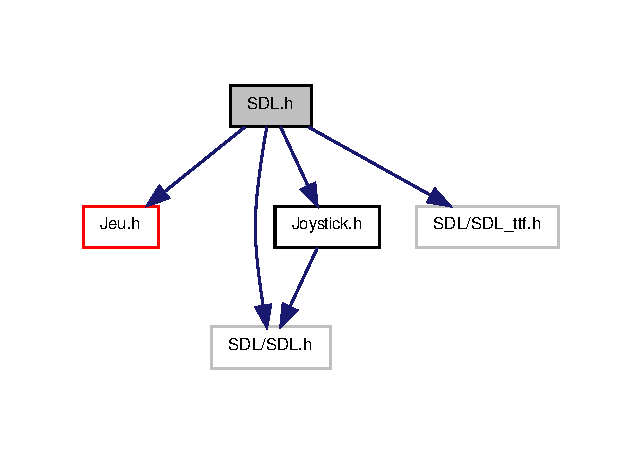
\includegraphics[width=308pt]{_s_d_l_8h__incl}
\end{center}
\end{figure}
Ce graphe montre quels fichiers incluent directement ou indirectement ce fichier \-:\nopagebreak
\begin{figure}[H]
\begin{center}
\leavevmode
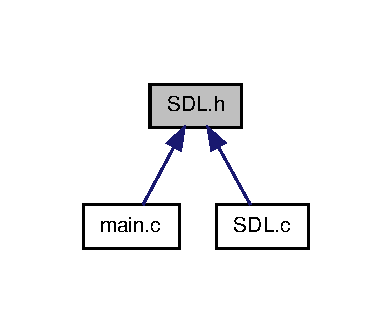
\includegraphics[width=176pt]{_s_d_l_8h__dep__incl}
\end{center}
\end{figure}
\subsection*{Structures de données}
\begin{DoxyCompactItemize}
\item 
struct \hyperlink{struct_s_d_l}{S\-D\-L}
\end{DoxyCompactItemize}
\subsection*{Fonctions}
\begin{DoxyCompactItemize}
\item 
\hyperlink{struct_jeu}{Jeu} $\ast$ \hyperlink{_s_d_l_8h_aa7223cb3ce4fe6f4c83d6a01adc66cbd}{S\-D\-L\-Get\-Jeu} (\hyperlink{struct_s_d_l}{S\-D\-L} $\ast$sdl)
\item 
S\-D\-L\-\_\-\-Surface $\ast$ \hyperlink{_s_d_l_8h_acca01b95fb78179e3051d8d411b8a9cd}{S\-D\-L\-Get\-Ieme\-Texture} (const \hyperlink{struct_s_d_l}{S\-D\-L} $\ast$sdl, unsigned int i)
\item 
\hyperlink{struct_manette}{Manette} $\ast$ \hyperlink{_s_d_l_8h_a0739253f7d24014416204f6d64c565b6}{S\-D\-L\-Get\-Ieme\-Manette} (const \hyperlink{struct_s_d_l}{S\-D\-L} $\ast$sdl, unsigned int i)
\item 
S\-D\-L\-\_\-\-Surface $\ast$ \hyperlink{_s_d_l_8h_a7596bb1c6890b99a64e59f6b732a2fe1}{S\-D\-L\-Get\-Textures} (const \hyperlink{struct_s_d_l}{S\-D\-L} $\ast$sdl)
\item 
void \hyperlink{_s_d_l_8h_a29faea1dc4bb87f4538e14d944b55a5e}{S\-D\-L\-Set\-Jeu} (\hyperlink{struct_s_d_l}{S\-D\-L} $\ast$sdl, \hyperlink{struct_jeu}{Jeu} $\ast$jeu)
\item 
void \hyperlink{_s_d_l_8h_ad7897b59aff5363840beb85766e25e47}{S\-D\-L\-Set\-Ieme\-Texture} (\hyperlink{struct_s_d_l}{S\-D\-L} $\ast$sdl, unsigned int i, S\-D\-L\-\_\-\-Surface $\ast$texture)
\item 
void \hyperlink{_s_d_l_8h_a7167f5c196fc5e167bfabde1a730e81d}{pause} ()
\item 
void \hyperlink{_s_d_l_8h_ab3ab37e752c937a11356bbe991509786}{S\-D\-L\-Constructeur} (\hyperlink{struct_s_d_l}{S\-D\-L} $\ast$sdl, \hyperlink{struct_jeu}{Jeu} $\ast$jeu, \hyperlink{struct_manette}{Manette} $\ast$mes\-Manettes)
\item 
void \hyperlink{_s_d_l_8h_a18f1617d8034417cd2f06cc9c4dbedf2}{S\-D\-L\-Destructeur} (\hyperlink{struct_s_d_l}{S\-D\-L} $\ast$sdl)
\item 
void \hyperlink{_s_d_l_8h_a894918515b5365e162d1c5e1214f97eb}{S\-D\-L\-Applique\-Surface} (S\-D\-L\-\_\-\-Surface $\ast$surface\-A, S\-D\-L\-\_\-\-Surface $\ast$surface\-B, int position\-X, int position\-Y)
\item 
void \hyperlink{_s_d_l_8h_a942e816249ca9bef39f4bbaada8d3daf}{S\-D\-L\-Affiche\-Jeu} (\hyperlink{struct_s_d_l}{S\-D\-L} $\ast$sdl, int $\ast$scores)
\item 
void \hyperlink{_s_d_l_8h_a0a164a520a75c594cf10cd3cfdca3814}{S\-D\-L\-Affiche\-Motos} (\hyperlink{struct_s_d_l}{S\-D\-L} $\ast$sdl)
\item 
void \hyperlink{_s_d_l_8h_a511761d608b92801c934aad221f762ce}{S\-D\-L\-Affiche\-Murs} (\hyperlink{struct_s_d_l}{S\-D\-L} $\ast$sdl)
\item 
void \hyperlink{_s_d_l_8h_a87530d8f5fdcb529d517fb86bc927e63}{S\-D\-L\-Affiche\-Interface} (\hyperlink{struct_s_d_l}{S\-D\-L} $\ast$sdl)
\item 
void \hyperlink{_s_d_l_8h_ac27595c16fe8fbd8ee635cb6c8d9ec40}{S\-D\-L\-Affiche\-Bonus} (\hyperlink{struct_s_d_l}{S\-D\-L} $\ast$sdl)
\item 
void \hyperlink{_s_d_l_8h_ad6a2da8e854839a096da5db6178b1356}{S\-D\-L\-Jeu\-Init\-N} (\hyperlink{struct_s_d_l}{S\-D\-L} $\ast$sdl, int $\ast$scores)
\item 
void \hyperlink{_s_d_l_8h_ab2b2544e3bfaa5cce134a84429e8dbd6}{S\-D\-L\-Affiche\-Textes} (\hyperlink{struct_s_d_l}{S\-D\-L} $\ast$sdl, char $\ast$chaine\-De\-Caractere, \hyperlink{_couleur_8h_aa304d0ca681f782b1d7735da33037dd7}{Couleur} une\-Couleur)
\item 
void \hyperlink{_s_d_l_8h_a1d801e3ea653b113f1868b6c8b1309f8}{S\-D\-L\-Affiche\-Scores} (\hyperlink{struct_s_d_l}{S\-D\-L} $\ast$sdl, int $\ast$scores)
\item 
void \hyperlink{_s_d_l_8h_a57b034bb0fbfd35900ad79a98b2be4bd}{S\-D\-L\-Boucle\-Jeu} (\hyperlink{struct_s_d_l}{S\-D\-L} $\ast$sdl, short int $\ast$jeu\-Re\-Init, int $\ast$scores)
\item 
S\-D\-L\-\_\-\-Surface $\ast$ \hyperlink{_s_d_l_8h_a36684beb5e5ec3f9397a2976415141b7}{S\-D\-L\-Charge\-Image} (const char $\ast$nomfichier)
\item 
void \hyperlink{_s_d_l_8h_a5307e0546a65557e28218096444fe16e}{S\-D\-L\-Action\-Manette} (\hyperlink{struct_joueur}{Joueur} $\ast$joueur, \hyperlink{_moto_8h_a224b9163917ac32fc95a60d8c1eec3aa}{Direction} direction, \hyperlink{struct_grid}{Grid} $\ast$grille)
\item 
void \hyperlink{_s_d_l_8h_a0de41957ce76d79bc06145340f5d2766}{S\-D\-L\-Test\-Regression} ()
\end{DoxyCompactItemize}


\subsection{Description détaillée}
\mbox{]} Module qui gère les affichage du jeu,ainsi que les manettes \begin{DoxyAuthor}{Auteur}
\{Antoine.\-C,Matthieu.\-B\} 
\end{DoxyAuthor}
\begin{DoxyVersion}{Version}
0.\-1 
\end{DoxyVersion}
\begin{DoxyDate}{Date}
19 mars 2013 
\end{DoxyDate}


Définition dans le fichier \hyperlink{_s_d_l_8h_source}{S\-D\-L.\-h}.



\subsection{Documentation des fonctions}
\hypertarget{_s_d_l_8h_a7167f5c196fc5e167bfabde1a730e81d}{\index{S\-D\-L.\-h@{S\-D\-L.\-h}!pause@{pause}}
\index{pause@{pause}!SDL.h@{S\-D\-L.\-h}}
\subsubsection[{pause}]{\setlength{\rightskip}{0pt plus 5cm}void pause (
\begin{DoxyParamCaption}
{}
\end{DoxyParamCaption}
)}}\label{_s_d_l_8h_a7167f5c196fc5e167bfabde1a730e81d}


Définition à la ligne 148 du fichier S\-D\-L.\-c.

\hypertarget{_s_d_l_8h_a5307e0546a65557e28218096444fe16e}{\index{S\-D\-L.\-h@{S\-D\-L.\-h}!S\-D\-L\-Action\-Manette@{S\-D\-L\-Action\-Manette}}
\index{S\-D\-L\-Action\-Manette@{S\-D\-L\-Action\-Manette}!SDL.h@{S\-D\-L.\-h}}
\subsubsection[{S\-D\-L\-Action\-Manette}]{\setlength{\rightskip}{0pt plus 5cm}void S\-D\-L\-Action\-Manette (
\begin{DoxyParamCaption}
\item[{{\bf Joueur} $\ast$}]{joueur, }
\item[{{\bf Direction}}]{direction, }
\item[{{\bf Grid} $\ast$}]{grille}
\end{DoxyParamCaption}
)}}\label{_s_d_l_8h_a5307e0546a65557e28218096444fe16e}


Définition à la ligne 566 du fichier S\-D\-L.\-c.

\hypertarget{_s_d_l_8h_ac27595c16fe8fbd8ee635cb6c8d9ec40}{\index{S\-D\-L.\-h@{S\-D\-L.\-h}!S\-D\-L\-Affiche\-Bonus@{S\-D\-L\-Affiche\-Bonus}}
\index{S\-D\-L\-Affiche\-Bonus@{S\-D\-L\-Affiche\-Bonus}!SDL.h@{S\-D\-L.\-h}}
\subsubsection[{S\-D\-L\-Affiche\-Bonus}]{\setlength{\rightskip}{0pt plus 5cm}void S\-D\-L\-Affiche\-Bonus (
\begin{DoxyParamCaption}
\item[{{\bf S\-D\-L} $\ast$}]{sdl}
\end{DoxyParamCaption}
)}}\label{_s_d_l_8h_ac27595c16fe8fbd8ee635cb6c8d9ec40}


Définition à la ligne 703 du fichier S\-D\-L.\-c.

\hypertarget{_s_d_l_8h_a87530d8f5fdcb529d517fb86bc927e63}{\index{S\-D\-L.\-h@{S\-D\-L.\-h}!S\-D\-L\-Affiche\-Interface@{S\-D\-L\-Affiche\-Interface}}
\index{S\-D\-L\-Affiche\-Interface@{S\-D\-L\-Affiche\-Interface}!SDL.h@{S\-D\-L.\-h}}
\subsubsection[{S\-D\-L\-Affiche\-Interface}]{\setlength{\rightskip}{0pt plus 5cm}void S\-D\-L\-Affiche\-Interface (
\begin{DoxyParamCaption}
\item[{{\bf S\-D\-L} $\ast$}]{sdl}
\end{DoxyParamCaption}
)}}\label{_s_d_l_8h_a87530d8f5fdcb529d517fb86bc927e63}


Définition à la ligne 723 du fichier S\-D\-L.\-c.

\hypertarget{_s_d_l_8h_a942e816249ca9bef39f4bbaada8d3daf}{\index{S\-D\-L.\-h@{S\-D\-L.\-h}!S\-D\-L\-Affiche\-Jeu@{S\-D\-L\-Affiche\-Jeu}}
\index{S\-D\-L\-Affiche\-Jeu@{S\-D\-L\-Affiche\-Jeu}!SDL.h@{S\-D\-L.\-h}}
\subsubsection[{S\-D\-L\-Affiche\-Jeu}]{\setlength{\rightskip}{0pt plus 5cm}void S\-D\-L\-Affiche\-Jeu (
\begin{DoxyParamCaption}
\item[{{\bf S\-D\-L} $\ast$}]{sdl, }
\item[{int $\ast$}]{scores}
\end{DoxyParamCaption}
)}}\label{_s_d_l_8h_a942e816249ca9bef39f4bbaada8d3daf}


Définition à la ligne 869 du fichier S\-D\-L.\-c.

\hypertarget{_s_d_l_8h_a0a164a520a75c594cf10cd3cfdca3814}{\index{S\-D\-L.\-h@{S\-D\-L.\-h}!S\-D\-L\-Affiche\-Motos@{S\-D\-L\-Affiche\-Motos}}
\index{S\-D\-L\-Affiche\-Motos@{S\-D\-L\-Affiche\-Motos}!SDL.h@{S\-D\-L.\-h}}
\subsubsection[{S\-D\-L\-Affiche\-Motos}]{\setlength{\rightskip}{0pt plus 5cm}void S\-D\-L\-Affiche\-Motos (
\begin{DoxyParamCaption}
\item[{{\bf S\-D\-L} $\ast$}]{sdl}
\end{DoxyParamCaption}
)}}\label{_s_d_l_8h_a0a164a520a75c594cf10cd3cfdca3814}


Définition à la ligne 642 du fichier S\-D\-L.\-c.

\hypertarget{_s_d_l_8h_a511761d608b92801c934aad221f762ce}{\index{S\-D\-L.\-h@{S\-D\-L.\-h}!S\-D\-L\-Affiche\-Murs@{S\-D\-L\-Affiche\-Murs}}
\index{S\-D\-L\-Affiche\-Murs@{S\-D\-L\-Affiche\-Murs}!SDL.h@{S\-D\-L.\-h}}
\subsubsection[{S\-D\-L\-Affiche\-Murs}]{\setlength{\rightskip}{0pt plus 5cm}void S\-D\-L\-Affiche\-Murs (
\begin{DoxyParamCaption}
\item[{{\bf S\-D\-L} $\ast$}]{sdl}
\end{DoxyParamCaption}
)}}\label{_s_d_l_8h_a511761d608b92801c934aad221f762ce}


Définition à la ligne 667 du fichier S\-D\-L.\-c.

\hypertarget{_s_d_l_8h_a1d801e3ea653b113f1868b6c8b1309f8}{\index{S\-D\-L.\-h@{S\-D\-L.\-h}!S\-D\-L\-Affiche\-Scores@{S\-D\-L\-Affiche\-Scores}}
\index{S\-D\-L\-Affiche\-Scores@{S\-D\-L\-Affiche\-Scores}!SDL.h@{S\-D\-L.\-h}}
\subsubsection[{S\-D\-L\-Affiche\-Scores}]{\setlength{\rightskip}{0pt plus 5cm}void S\-D\-L\-Affiche\-Scores (
\begin{DoxyParamCaption}
\item[{{\bf S\-D\-L} $\ast$}]{sdl, }
\item[{int $\ast$}]{scores}
\end{DoxyParamCaption}
)}}\label{_s_d_l_8h_a1d801e3ea653b113f1868b6c8b1309f8}
$<$affichage de la ligne supérieure

$<$affichage de la ligne inférieure 

Définition à la ligne 816 du fichier S\-D\-L.\-c.

\hypertarget{_s_d_l_8h_ab2b2544e3bfaa5cce134a84429e8dbd6}{\index{S\-D\-L.\-h@{S\-D\-L.\-h}!S\-D\-L\-Affiche\-Textes@{S\-D\-L\-Affiche\-Textes}}
\index{S\-D\-L\-Affiche\-Textes@{S\-D\-L\-Affiche\-Textes}!SDL.h@{S\-D\-L.\-h}}
\subsubsection[{S\-D\-L\-Affiche\-Textes}]{\setlength{\rightskip}{0pt plus 5cm}void S\-D\-L\-Affiche\-Textes (
\begin{DoxyParamCaption}
\item[{{\bf S\-D\-L} $\ast$}]{sdl, }
\item[{char $\ast$}]{chaine\-De\-Caractere, }
\item[{{\bf Couleur}}]{une\-Couleur}
\end{DoxyParamCaption}
)}}\label{_s_d_l_8h_ab2b2544e3bfaa5cce134a84429e8dbd6}


Définition à la ligne 743 du fichier S\-D\-L.\-c.

\hypertarget{_s_d_l_8h_a894918515b5365e162d1c5e1214f97eb}{\index{S\-D\-L.\-h@{S\-D\-L.\-h}!S\-D\-L\-Applique\-Surface@{S\-D\-L\-Applique\-Surface}}
\index{S\-D\-L\-Applique\-Surface@{S\-D\-L\-Applique\-Surface}!SDL.h@{S\-D\-L.\-h}}
\subsubsection[{S\-D\-L\-Applique\-Surface}]{\setlength{\rightskip}{0pt plus 5cm}void S\-D\-L\-Applique\-Surface (
\begin{DoxyParamCaption}
\item[{S\-D\-L\-\_\-\-Surface $\ast$}]{surface\-A, }
\item[{S\-D\-L\-\_\-\-Surface $\ast$}]{surface\-B, }
\item[{int}]{position\-X, }
\item[{int}]{position\-Y}
\end{DoxyParamCaption}
)}}\label{_s_d_l_8h_a894918515b5365e162d1c5e1214f97eb}
!$<$ Make a temporary rectangle to hold the offsets

!$<$ Give the offsets to the rectangle

!$<$ Blit the surface 

Définition à la ligne 56 du fichier S\-D\-L.\-c.

\hypertarget{_s_d_l_8h_a57b034bb0fbfd35900ad79a98b2be4bd}{\index{S\-D\-L.\-h@{S\-D\-L.\-h}!S\-D\-L\-Boucle\-Jeu@{S\-D\-L\-Boucle\-Jeu}}
\index{S\-D\-L\-Boucle\-Jeu@{S\-D\-L\-Boucle\-Jeu}!SDL.h@{S\-D\-L.\-h}}
\subsubsection[{S\-D\-L\-Boucle\-Jeu}]{\setlength{\rightskip}{0pt plus 5cm}void S\-D\-L\-Boucle\-Jeu (
\begin{DoxyParamCaption}
\item[{{\bf S\-D\-L} $\ast$}]{sdl, }
\item[{short int $\ast$}]{jeu\-Re\-Init, }
\item[{int $\ast$}]{scores}
\end{DoxyParamCaption}
)}}\label{_s_d_l_8h_a57b034bb0fbfd35900ad79a98b2be4bd}
!$<$Si le jeu a renvoyé un nouveau commentaire 

Définition à la ligne 389 du fichier S\-D\-L.\-c.

\hypertarget{_s_d_l_8h_a36684beb5e5ec3f9397a2976415141b7}{\index{S\-D\-L.\-h@{S\-D\-L.\-h}!S\-D\-L\-Charge\-Image@{S\-D\-L\-Charge\-Image}}
\index{S\-D\-L\-Charge\-Image@{S\-D\-L\-Charge\-Image}!SDL.h@{S\-D\-L.\-h}}
\subsubsection[{S\-D\-L\-Charge\-Image}]{\setlength{\rightskip}{0pt plus 5cm}S\-D\-L\-\_\-\-Surface$\ast$ S\-D\-L\-Charge\-Image (
\begin{DoxyParamCaption}
\item[{const char $\ast$}]{nomfichier}
\end{DoxyParamCaption}
)}}\label{_s_d_l_8h_a36684beb5e5ec3f9397a2976415141b7}
!$<$ Temporary storage for the image that's loaded

!$<$ Load the image

!$<$ If nothing went wrong in loading the image

!$<$ Return the optimized image 

Définition à la ligne 41 du fichier S\-D\-L.\-c.

\hypertarget{_s_d_l_8h_ab3ab37e752c937a11356bbe991509786}{\index{S\-D\-L.\-h@{S\-D\-L.\-h}!S\-D\-L\-Constructeur@{S\-D\-L\-Constructeur}}
\index{S\-D\-L\-Constructeur@{S\-D\-L\-Constructeur}!SDL.h@{S\-D\-L.\-h}}
\subsubsection[{S\-D\-L\-Constructeur}]{\setlength{\rightskip}{0pt plus 5cm}void S\-D\-L\-Constructeur (
\begin{DoxyParamCaption}
\item[{{\bf S\-D\-L} $\ast$}]{sdl, }
\item[{{\bf Jeu} $\ast$}]{jeu, }
\item[{{\bf Manette} $\ast$}]{mes\-Manettes}
\end{DoxyParamCaption}
)}}\label{_s_d_l_8h_ab3ab37e752c937a11356bbe991509786}


Définition à la ligne 70 du fichier S\-D\-L.\-c.

\hypertarget{_s_d_l_8h_a18f1617d8034417cd2f06cc9c4dbedf2}{\index{S\-D\-L.\-h@{S\-D\-L.\-h}!S\-D\-L\-Destructeur@{S\-D\-L\-Destructeur}}
\index{S\-D\-L\-Destructeur@{S\-D\-L\-Destructeur}!SDL.h@{S\-D\-L.\-h}}
\subsubsection[{S\-D\-L\-Destructeur}]{\setlength{\rightskip}{0pt plus 5cm}void S\-D\-L\-Destructeur (
\begin{DoxyParamCaption}
\item[{{\bf S\-D\-L} $\ast$}]{sdl}
\end{DoxyParamCaption}
)}}\label{_s_d_l_8h_a18f1617d8034417cd2f06cc9c4dbedf2}


Définition à la ligne 132 du fichier S\-D\-L.\-c.

\hypertarget{_s_d_l_8h_a0739253f7d24014416204f6d64c565b6}{\index{S\-D\-L.\-h@{S\-D\-L.\-h}!S\-D\-L\-Get\-Ieme\-Manette@{S\-D\-L\-Get\-Ieme\-Manette}}
\index{S\-D\-L\-Get\-Ieme\-Manette@{S\-D\-L\-Get\-Ieme\-Manette}!SDL.h@{S\-D\-L.\-h}}
\subsubsection[{S\-D\-L\-Get\-Ieme\-Manette}]{\setlength{\rightskip}{0pt plus 5cm}{\bf Manette}$\ast$ S\-D\-L\-Get\-Ieme\-Manette (
\begin{DoxyParamCaption}
\item[{const {\bf S\-D\-L} $\ast$}]{sdl, }
\item[{unsigned int}]{i}
\end{DoxyParamCaption}
)}}\label{_s_d_l_8h_a0739253f7d24014416204f6d64c565b6}


Définition à la ligne 24 du fichier S\-D\-L.\-c.

\hypertarget{_s_d_l_8h_acca01b95fb78179e3051d8d411b8a9cd}{\index{S\-D\-L.\-h@{S\-D\-L.\-h}!S\-D\-L\-Get\-Ieme\-Texture@{S\-D\-L\-Get\-Ieme\-Texture}}
\index{S\-D\-L\-Get\-Ieme\-Texture@{S\-D\-L\-Get\-Ieme\-Texture}!SDL.h@{S\-D\-L.\-h}}
\subsubsection[{S\-D\-L\-Get\-Ieme\-Texture}]{\setlength{\rightskip}{0pt plus 5cm}S\-D\-L\-\_\-\-Surface$\ast$ S\-D\-L\-Get\-Ieme\-Texture (
\begin{DoxyParamCaption}
\item[{const {\bf S\-D\-L} $\ast$}]{sdl, }
\item[{unsigned int}]{i}
\end{DoxyParamCaption}
)}}\label{_s_d_l_8h_acca01b95fb78179e3051d8d411b8a9cd}


Définition à la ligne 21 du fichier S\-D\-L.\-c.

\hypertarget{_s_d_l_8h_aa7223cb3ce4fe6f4c83d6a01adc66cbd}{\index{S\-D\-L.\-h@{S\-D\-L.\-h}!S\-D\-L\-Get\-Jeu@{S\-D\-L\-Get\-Jeu}}
\index{S\-D\-L\-Get\-Jeu@{S\-D\-L\-Get\-Jeu}!SDL.h@{S\-D\-L.\-h}}
\subsubsection[{S\-D\-L\-Get\-Jeu}]{\setlength{\rightskip}{0pt plus 5cm}{\bf Jeu}$\ast$ S\-D\-L\-Get\-Jeu (
\begin{DoxyParamCaption}
\item[{{\bf S\-D\-L} $\ast$}]{sdl}
\end{DoxyParamCaption}
)}}\label{_s_d_l_8h_aa7223cb3ce4fe6f4c83d6a01adc66cbd}


Définition à la ligne 18 du fichier S\-D\-L.\-c.

\hypertarget{_s_d_l_8h_a7596bb1c6890b99a64e59f6b732a2fe1}{\index{S\-D\-L.\-h@{S\-D\-L.\-h}!S\-D\-L\-Get\-Textures@{S\-D\-L\-Get\-Textures}}
\index{S\-D\-L\-Get\-Textures@{S\-D\-L\-Get\-Textures}!SDL.h@{S\-D\-L.\-h}}
\subsubsection[{S\-D\-L\-Get\-Textures}]{\setlength{\rightskip}{0pt plus 5cm}S\-D\-L\-\_\-\-Surface$\ast$ S\-D\-L\-Get\-Textures (
\begin{DoxyParamCaption}
\item[{const {\bf S\-D\-L} $\ast$}]{sdl}
\end{DoxyParamCaption}
)}}\label{_s_d_l_8h_a7596bb1c6890b99a64e59f6b732a2fe1}


Définition à la ligne 27 du fichier S\-D\-L.\-c.

\hypertarget{_s_d_l_8h_ad6a2da8e854839a096da5db6178b1356}{\index{S\-D\-L.\-h@{S\-D\-L.\-h}!S\-D\-L\-Jeu\-Init\-N@{S\-D\-L\-Jeu\-Init\-N}}
\index{S\-D\-L\-Jeu\-Init\-N@{S\-D\-L\-Jeu\-Init\-N}!SDL.h@{S\-D\-L.\-h}}
\subsubsection[{S\-D\-L\-Jeu\-Init\-N}]{\setlength{\rightskip}{0pt plus 5cm}void S\-D\-L\-Jeu\-Init\-N (
\begin{DoxyParamCaption}
\item[{{\bf S\-D\-L} $\ast$}]{sdl, }
\item[{int $\ast$}]{scores}
\end{DoxyParamCaption}
)}}\label{_s_d_l_8h_ad6a2da8e854839a096da5db6178b1356}


Définition à la ligne 164 du fichier S\-D\-L.\-c.

\hypertarget{_s_d_l_8h_ad7897b59aff5363840beb85766e25e47}{\index{S\-D\-L.\-h@{S\-D\-L.\-h}!S\-D\-L\-Set\-Ieme\-Texture@{S\-D\-L\-Set\-Ieme\-Texture}}
\index{S\-D\-L\-Set\-Ieme\-Texture@{S\-D\-L\-Set\-Ieme\-Texture}!SDL.h@{S\-D\-L.\-h}}
\subsubsection[{S\-D\-L\-Set\-Ieme\-Texture}]{\setlength{\rightskip}{0pt plus 5cm}void S\-D\-L\-Set\-Ieme\-Texture (
\begin{DoxyParamCaption}
\item[{{\bf S\-D\-L} $\ast$}]{sdl, }
\item[{unsigned int}]{i, }
\item[{S\-D\-L\-\_\-\-Surface $\ast$}]{texture}
\end{DoxyParamCaption}
)}}\label{_s_d_l_8h_ad7897b59aff5363840beb85766e25e47}


Définition à la ligne 34 du fichier S\-D\-L.\-c.

\hypertarget{_s_d_l_8h_a29faea1dc4bb87f4538e14d944b55a5e}{\index{S\-D\-L.\-h@{S\-D\-L.\-h}!S\-D\-L\-Set\-Jeu@{S\-D\-L\-Set\-Jeu}}
\index{S\-D\-L\-Set\-Jeu@{S\-D\-L\-Set\-Jeu}!SDL.h@{S\-D\-L.\-h}}
\subsubsection[{S\-D\-L\-Set\-Jeu}]{\setlength{\rightskip}{0pt plus 5cm}void S\-D\-L\-Set\-Jeu (
\begin{DoxyParamCaption}
\item[{{\bf S\-D\-L} $\ast$}]{sdl, }
\item[{{\bf Jeu} $\ast$}]{jeu}
\end{DoxyParamCaption}
)}}\label{_s_d_l_8h_a29faea1dc4bb87f4538e14d944b55a5e}


Définition à la ligne 31 du fichier S\-D\-L.\-c.

\hypertarget{_s_d_l_8h_a0de41957ce76d79bc06145340f5d2766}{\index{S\-D\-L.\-h@{S\-D\-L.\-h}!S\-D\-L\-Test\-Regression@{S\-D\-L\-Test\-Regression}}
\index{S\-D\-L\-Test\-Regression@{S\-D\-L\-Test\-Regression}!SDL.h@{S\-D\-L.\-h}}
\subsubsection[{S\-D\-L\-Test\-Regression}]{\setlength{\rightskip}{0pt plus 5cm}void S\-D\-L\-Test\-Regression (
\begin{DoxyParamCaption}
{}
\end{DoxyParamCaption}
)}}\label{_s_d_l_8h_a0de41957ce76d79bc06145340f5d2766}
procédure qui teste le Module 

Définition à la ligne 880 du fichier S\-D\-L.\-c.


\hypertarget{_tableau_dynamique_entier_8c}{\section{Référence du fichier Tableau\-Dynamique\-Entier.\-c}
\label{_tableau_dynamique_entier_8c}\index{Tableau\-Dynamique\-Entier.\-c@{Tableau\-Dynamique\-Entier.\-c}}
}
{\ttfamily \#include \char`\"{}Tableau\-Dynamique\-Entier.\-h\char`\"{}}\\*
{\ttfamily \#include $<$stdlib.\-h$>$}\\*
Graphe des dépendances par inclusion de Tableau\-Dynamique\-Entier.\-c\-:\nopagebreak
\begin{figure}[H]
\begin{center}
\leavevmode
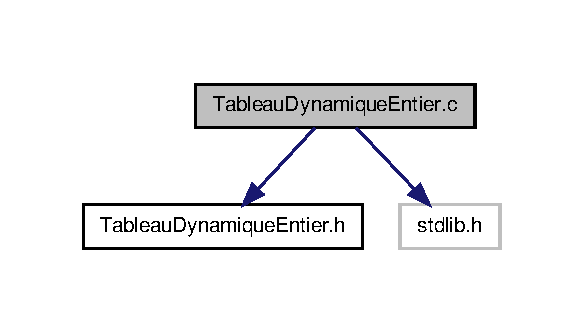
\includegraphics[width=252pt]{_tableau_dynamique_entier_8c__incl}
\end{center}
\end{figure}
\subsection*{Fonctions}
\begin{DoxyCompactItemize}
\item 
unsigned int \hyperlink{_tableau_dynamique_entier_8c_ab6a8726196a5f20917c43d82c7023b20}{Tab\-Dyn\-Entier\-Get\-Capacite} (const \hyperlink{struct_tableau_dynamique_entier}{Tableau\-Dynamique\-Entier} $\ast$Tab\-Dyn\-Entier)
\item 
unsigned int \hyperlink{_tableau_dynamique_entier_8c_a136e17ac632e98e56b37ec94cd375eac}{Tab\-Dyn\-Entier\-Get\-Taille\-\_\-utilisee} (const \hyperlink{struct_tableau_dynamique_entier}{Tableau\-Dynamique\-Entier} $\ast$Tab\-Dyn\-Entier)
\item 
int $\ast$ \hyperlink{_tableau_dynamique_entier_8c_a6eaf357a41e8d4fd4b4ea4ff62a6f6ed}{Tab\-Dyn\-Entier\-Get\-Ad} (const \hyperlink{struct_tableau_dynamique_entier}{Tableau\-Dynamique\-Entier} $\ast$Tab\-Dyn\-Entier)
\item 
void \hyperlink{_tableau_dynamique_entier_8c_ad954cdcf51e383884837bf7da3f46ab0}{Tab\-Dyn\-Entier\-Set\-Capacite} (\hyperlink{struct_tableau_dynamique_entier}{Tableau\-Dynamique\-Entier} $\ast$Tab\-Dyn\-Entier, unsigned int capacite)
\item 
void \hyperlink{_tableau_dynamique_entier_8c_a72608244b7a6a4af534abe48f3b7fbe2}{Tab\-Dyn\-Entier\-Set\-Taille\-\_\-utilisee} (\hyperlink{struct_tableau_dynamique_entier}{Tableau\-Dynamique\-Entier} $\ast$Tab\-Dyn\-Entier, unsigned int taille)
\item 
void \hyperlink{_tableau_dynamique_entier_8c_a943ad435f0921f55fad1004b7201819f}{Tab\-Dyn\-Entier\-Set\-Ad} (\hyperlink{struct_tableau_dynamique_entier}{Tableau\-Dynamique\-Entier} $\ast$Tab\-Dyn\-Entier, int $\ast$ad)
\item 
void \hyperlink{_tableau_dynamique_entier_8c_afe49c3b20d8e7e9075c163b5e4c6e9dc}{initialiser\-Tab\-Dyn\-Entier} (\hyperlink{struct_tableau_dynamique_entier}{Tableau\-Dynamique\-Entier} $\ast$t)
\item 
void \hyperlink{_tableau_dynamique_entier_8c_ac301681c4b3f4bce74fd9773f1da9ef6}{testament\-Tab\-Dyn\-Entier} (\hyperlink{struct_tableau_dynamique_entier}{Tableau\-Dynamique\-Entier} $\ast$t)
\item 
void \hyperlink{_tableau_dynamique_entier_8c_afe79a1dd09df3d0119679d87f20aec6f}{ajouter\-Element\-Tab\-Dyn\-Entier} (\hyperlink{struct_tableau_dynamique_entier}{Tableau\-Dynamique\-Entier} $\ast$t, int e)
\item 
int \hyperlink{_tableau_dynamique_entier_8c_ad273850f79af1e74ecd32971b08fe7d8}{valeur\-Ieme\-Element\-Tab\-Dyn\-Entier} (const \hyperlink{struct_tableau_dynamique_entier}{Tableau\-Dynamique\-Entier} $\ast$t, unsigned int i)
\item 
int $\ast$ \hyperlink{_tableau_dynamique_entier_8c_ad0efdf4c23b94918071fca8711446c98}{adresse\-Ieme\-Element\-Tab\-Dyn\-Entier} (const \hyperlink{struct_tableau_dynamique_entier}{Tableau\-Dynamique\-Entier} $\ast$t, unsigned int i)
\item 
void \hyperlink{_tableau_dynamique_entier_8c_a6b328364f2565029828b234d44d0bd4b}{modifier\-Valeur\-Ieme\-Element\-Tab\-Dyn\-Entier} (\hyperlink{struct_tableau_dynamique_entier}{Tableau\-Dynamique\-Entier} $\ast$t, int e, unsigned int i)
\item 
void \hyperlink{_tableau_dynamique_entier_8c_aebe791fb2f38ce5909b196ee1f1788e1}{supprimer\-Element\-Tab\-Dyn\-Entier} (\hyperlink{struct_tableau_dynamique_entier}{Tableau\-Dynamique\-Entier} $\ast$t, int position)
\end{DoxyCompactItemize}


\subsection{Description détaillée}
\mbox{]} Module qui gère les tableaux dynamiques d'entier \begin{DoxyAuthor}{Auteur}
\{Antoine.\-C,Matthieu.\-B\} 
\end{DoxyAuthor}
\begin{DoxyVersion}{Version}
1.\-0 
\end{DoxyVersion}
\begin{DoxyDate}{Date}
19 mars 2013 
\end{DoxyDate}


Définition dans le fichier \hyperlink{_tableau_dynamique_entier_8c_source}{Tableau\-Dynamique\-Entier.\-c}.



\subsection{Documentation des fonctions}
\hypertarget{_tableau_dynamique_entier_8c_ad0efdf4c23b94918071fca8711446c98}{\index{Tableau\-Dynamique\-Entier.\-c@{Tableau\-Dynamique\-Entier.\-c}!adresse\-Ieme\-Element\-Tab\-Dyn\-Entier@{adresse\-Ieme\-Element\-Tab\-Dyn\-Entier}}
\index{adresse\-Ieme\-Element\-Tab\-Dyn\-Entier@{adresse\-Ieme\-Element\-Tab\-Dyn\-Entier}!TableauDynamiqueEntier.c@{Tableau\-Dynamique\-Entier.\-c}}
\subsubsection[{adresse\-Ieme\-Element\-Tab\-Dyn\-Entier}]{\setlength{\rightskip}{0pt plus 5cm}int$\ast$ adresse\-Ieme\-Element\-Tab\-Dyn\-Entier (
\begin{DoxyParamCaption}
\item[{const {\bf Tableau\-Dynamique\-Entier} $\ast$}]{t, }
\item[{unsigned int}]{i}
\end{DoxyParamCaption}
)}}\label{_tableau_dynamique_entier_8c_ad0efdf4c23b94918071fca8711446c98}
Precondition \-: t prealablement initialise, 0 $<$= i $<$ taille\-Utilisee(t) Resultat \-: retourne l'adresse du i+1eme Element\-T\-D de t 

Définition à la ligne 80 du fichier Tableau\-Dynamique\-Entier.\-c.

\hypertarget{_tableau_dynamique_entier_8c_afe79a1dd09df3d0119679d87f20aec6f}{\index{Tableau\-Dynamique\-Entier.\-c@{Tableau\-Dynamique\-Entier.\-c}!ajouter\-Element\-Tab\-Dyn\-Entier@{ajouter\-Element\-Tab\-Dyn\-Entier}}
\index{ajouter\-Element\-Tab\-Dyn\-Entier@{ajouter\-Element\-Tab\-Dyn\-Entier}!TableauDynamiqueEntier.c@{Tableau\-Dynamique\-Entier.\-c}}
\subsubsection[{ajouter\-Element\-Tab\-Dyn\-Entier}]{\setlength{\rightskip}{0pt plus 5cm}void ajouter\-Element\-Tab\-Dyn\-Entier (
\begin{DoxyParamCaption}
\item[{{\bf Tableau\-Dynamique\-Entier} $\ast$}]{t, }
\item[{int}]{e}
\end{DoxyParamCaption}
)}}\label{_tableau_dynamique_entier_8c_afe79a1dd09df3d0119679d87f20aec6f}
Precondition \-: t prealablement initialise Postcondition \-: L'element e est ajoute dans la premiere alveole inutilisee du tableau, la taille utilisee est incrementee de 1. Doublement de la capacite de t, si necessaire. 

Définition à la ligne 55 du fichier Tableau\-Dynamique\-Entier.\-c.

\hypertarget{_tableau_dynamique_entier_8c_afe49c3b20d8e7e9075c163b5e4c6e9dc}{\index{Tableau\-Dynamique\-Entier.\-c@{Tableau\-Dynamique\-Entier.\-c}!initialiser\-Tab\-Dyn\-Entier@{initialiser\-Tab\-Dyn\-Entier}}
\index{initialiser\-Tab\-Dyn\-Entier@{initialiser\-Tab\-Dyn\-Entier}!TableauDynamiqueEntier.c@{Tableau\-Dynamique\-Entier.\-c}}
\subsubsection[{initialiser\-Tab\-Dyn\-Entier}]{\setlength{\rightskip}{0pt plus 5cm}void initialiser\-Tab\-Dyn\-Entier (
\begin{DoxyParamCaption}
\item[{{\bf Tableau\-Dynamique\-Entier} $\ast$}]{t}
\end{DoxyParamCaption}
)}}\label{_tableau_dynamique_entier_8c_afe49c3b20d8e7e9075c163b5e4c6e9dc}
Precondition \-: t non prealablement initialise Postcondition \-: t initialise a une alveole vide (taille utilisee nulle) 

Définition à la ligne 35 du fichier Tableau\-Dynamique\-Entier.\-c.

\hypertarget{_tableau_dynamique_entier_8c_a6b328364f2565029828b234d44d0bd4b}{\index{Tableau\-Dynamique\-Entier.\-c@{Tableau\-Dynamique\-Entier.\-c}!modifier\-Valeur\-Ieme\-Element\-Tab\-Dyn\-Entier@{modifier\-Valeur\-Ieme\-Element\-Tab\-Dyn\-Entier}}
\index{modifier\-Valeur\-Ieme\-Element\-Tab\-Dyn\-Entier@{modifier\-Valeur\-Ieme\-Element\-Tab\-Dyn\-Entier}!TableauDynamiqueEntier.c@{Tableau\-Dynamique\-Entier.\-c}}
\subsubsection[{modifier\-Valeur\-Ieme\-Element\-Tab\-Dyn\-Entier}]{\setlength{\rightskip}{0pt plus 5cm}void modifier\-Valeur\-Ieme\-Element\-Tab\-Dyn\-Entier (
\begin{DoxyParamCaption}
\item[{{\bf Tableau\-Dynamique\-Entier} $\ast$}]{t, }
\item[{int}]{e, }
\item[{unsigned int}]{i}
\end{DoxyParamCaption}
)}}\label{_tableau_dynamique_entier_8c_a6b328364f2565029828b234d44d0bd4b}
Precondition \-: t prealablement initialise et 0 $<$= i $<$ taille\-Utilisee(t) Postcondition \-: le i+1eme Element\-T\-D de t vaut e 

Définition à la ligne 87 du fichier Tableau\-Dynamique\-Entier.\-c.

\hypertarget{_tableau_dynamique_entier_8c_aebe791fb2f38ce5909b196ee1f1788e1}{\index{Tableau\-Dynamique\-Entier.\-c@{Tableau\-Dynamique\-Entier.\-c}!supprimer\-Element\-Tab\-Dyn\-Entier@{supprimer\-Element\-Tab\-Dyn\-Entier}}
\index{supprimer\-Element\-Tab\-Dyn\-Entier@{supprimer\-Element\-Tab\-Dyn\-Entier}!TableauDynamiqueEntier.c@{Tableau\-Dynamique\-Entier.\-c}}
\subsubsection[{supprimer\-Element\-Tab\-Dyn\-Entier}]{\setlength{\rightskip}{0pt plus 5cm}void supprimer\-Element\-Tab\-Dyn\-Entier (
\begin{DoxyParamCaption}
\item[{{\bf Tableau\-Dynamique\-Entier} $\ast$}]{t, }
\item[{int}]{position}
\end{DoxyParamCaption}
)}}\label{_tableau_dynamique_entier_8c_aebe791fb2f38ce5909b196ee1f1788e1}
Precondition \-: t prealablement initialise et non vide Postcondition \-: la taille utilisee du tableau est decrementee de 1. Si taille\-Utilisee $<$ capacite/3, alors on divise la capacité par 2. 

Définition à la ligne 97 du fichier Tableau\-Dynamique\-Entier.\-c.

\hypertarget{_tableau_dynamique_entier_8c_a6eaf357a41e8d4fd4b4ea4ff62a6f6ed}{\index{Tableau\-Dynamique\-Entier.\-c@{Tableau\-Dynamique\-Entier.\-c}!Tab\-Dyn\-Entier\-Get\-Ad@{Tab\-Dyn\-Entier\-Get\-Ad}}
\index{Tab\-Dyn\-Entier\-Get\-Ad@{Tab\-Dyn\-Entier\-Get\-Ad}!TableauDynamiqueEntier.c@{Tableau\-Dynamique\-Entier.\-c}}
\subsubsection[{Tab\-Dyn\-Entier\-Get\-Ad}]{\setlength{\rightskip}{0pt plus 5cm}int$\ast$ Tab\-Dyn\-Entier\-Get\-Ad (
\begin{DoxyParamCaption}
\item[{const {\bf Tableau\-Dynamique\-Entier} $\ast$}]{Tab\-Dyn\-Entier}
\end{DoxyParamCaption}
)}}\label{_tableau_dynamique_entier_8c_a6eaf357a41e8d4fd4b4ea4ff62a6f6ed}
assesseur de ad 

Définition à la ligne 18 du fichier Tableau\-Dynamique\-Entier.\-c.

\hypertarget{_tableau_dynamique_entier_8c_ab6a8726196a5f20917c43d82c7023b20}{\index{Tableau\-Dynamique\-Entier.\-c@{Tableau\-Dynamique\-Entier.\-c}!Tab\-Dyn\-Entier\-Get\-Capacite@{Tab\-Dyn\-Entier\-Get\-Capacite}}
\index{Tab\-Dyn\-Entier\-Get\-Capacite@{Tab\-Dyn\-Entier\-Get\-Capacite}!TableauDynamiqueEntier.c@{Tableau\-Dynamique\-Entier.\-c}}
\subsubsection[{Tab\-Dyn\-Entier\-Get\-Capacite}]{\setlength{\rightskip}{0pt plus 5cm}unsigned int Tab\-Dyn\-Entier\-Get\-Capacite (
\begin{DoxyParamCaption}
\item[{const {\bf Tableau\-Dynamique\-Entier} $\ast$}]{Tab\-Dyn\-Entier}
\end{DoxyParamCaption}
)}}\label{_tableau_dynamique_entier_8c_ab6a8726196a5f20917c43d82c7023b20}
assesseur de capacite 

Définition à la ligne 12 du fichier Tableau\-Dynamique\-Entier.\-c.

\hypertarget{_tableau_dynamique_entier_8c_a136e17ac632e98e56b37ec94cd375eac}{\index{Tableau\-Dynamique\-Entier.\-c@{Tableau\-Dynamique\-Entier.\-c}!Tab\-Dyn\-Entier\-Get\-Taille\-\_\-utilisee@{Tab\-Dyn\-Entier\-Get\-Taille\-\_\-utilisee}}
\index{Tab\-Dyn\-Entier\-Get\-Taille\-\_\-utilisee@{Tab\-Dyn\-Entier\-Get\-Taille\-\_\-utilisee}!TableauDynamiqueEntier.c@{Tableau\-Dynamique\-Entier.\-c}}
\subsubsection[{Tab\-Dyn\-Entier\-Get\-Taille\-\_\-utilisee}]{\setlength{\rightskip}{0pt plus 5cm}unsigned int Tab\-Dyn\-Entier\-Get\-Taille\-\_\-utilisee (
\begin{DoxyParamCaption}
\item[{const {\bf Tableau\-Dynamique\-Entier} $\ast$}]{Tab\-Dyn\-Entier}
\end{DoxyParamCaption}
)}}\label{_tableau_dynamique_entier_8c_a136e17ac632e98e56b37ec94cd375eac}
assesseur de taille\-\_\-utilisee 

Définition à la ligne 15 du fichier Tableau\-Dynamique\-Entier.\-c.

\hypertarget{_tableau_dynamique_entier_8c_a943ad435f0921f55fad1004b7201819f}{\index{Tableau\-Dynamique\-Entier.\-c@{Tableau\-Dynamique\-Entier.\-c}!Tab\-Dyn\-Entier\-Set\-Ad@{Tab\-Dyn\-Entier\-Set\-Ad}}
\index{Tab\-Dyn\-Entier\-Set\-Ad@{Tab\-Dyn\-Entier\-Set\-Ad}!TableauDynamiqueEntier.c@{Tableau\-Dynamique\-Entier.\-c}}
\subsubsection[{Tab\-Dyn\-Entier\-Set\-Ad}]{\setlength{\rightskip}{0pt plus 5cm}void Tab\-Dyn\-Entier\-Set\-Ad (
\begin{DoxyParamCaption}
\item[{{\bf Tableau\-Dynamique\-Entier} $\ast$}]{Tab\-Dyn\-Entier, }
\item[{int $\ast$}]{ad}
\end{DoxyParamCaption}
)}}\label{_tableau_dynamique_entier_8c_a943ad435f0921f55fad1004b7201819f}
mutateur de ad 

Définition à la ligne 28 du fichier Tableau\-Dynamique\-Entier.\-c.

\hypertarget{_tableau_dynamique_entier_8c_ad954cdcf51e383884837bf7da3f46ab0}{\index{Tableau\-Dynamique\-Entier.\-c@{Tableau\-Dynamique\-Entier.\-c}!Tab\-Dyn\-Entier\-Set\-Capacite@{Tab\-Dyn\-Entier\-Set\-Capacite}}
\index{Tab\-Dyn\-Entier\-Set\-Capacite@{Tab\-Dyn\-Entier\-Set\-Capacite}!TableauDynamiqueEntier.c@{Tableau\-Dynamique\-Entier.\-c}}
\subsubsection[{Tab\-Dyn\-Entier\-Set\-Capacite}]{\setlength{\rightskip}{0pt plus 5cm}void Tab\-Dyn\-Entier\-Set\-Capacite (
\begin{DoxyParamCaption}
\item[{{\bf Tableau\-Dynamique\-Entier} $\ast$}]{Tab\-Dyn\-Entier, }
\item[{unsigned int}]{capacite}
\end{DoxyParamCaption}
)}}\label{_tableau_dynamique_entier_8c_ad954cdcf51e383884837bf7da3f46ab0}
mutateur de capacite 

Définition à la ligne 22 du fichier Tableau\-Dynamique\-Entier.\-c.

\hypertarget{_tableau_dynamique_entier_8c_a72608244b7a6a4af534abe48f3b7fbe2}{\index{Tableau\-Dynamique\-Entier.\-c@{Tableau\-Dynamique\-Entier.\-c}!Tab\-Dyn\-Entier\-Set\-Taille\-\_\-utilisee@{Tab\-Dyn\-Entier\-Set\-Taille\-\_\-utilisee}}
\index{Tab\-Dyn\-Entier\-Set\-Taille\-\_\-utilisee@{Tab\-Dyn\-Entier\-Set\-Taille\-\_\-utilisee}!TableauDynamiqueEntier.c@{Tableau\-Dynamique\-Entier.\-c}}
\subsubsection[{Tab\-Dyn\-Entier\-Set\-Taille\-\_\-utilisee}]{\setlength{\rightskip}{0pt plus 5cm}void Tab\-Dyn\-Entier\-Set\-Taille\-\_\-utilisee (
\begin{DoxyParamCaption}
\item[{{\bf Tableau\-Dynamique\-Entier} $\ast$}]{Tab\-Dyn\-Entier, }
\item[{unsigned int}]{taille}
\end{DoxyParamCaption}
)}}\label{_tableau_dynamique_entier_8c_a72608244b7a6a4af534abe48f3b7fbe2}
mutateur de taille\-\_\-utilisee 

Définition à la ligne 25 du fichier Tableau\-Dynamique\-Entier.\-c.

\hypertarget{_tableau_dynamique_entier_8c_ac301681c4b3f4bce74fd9773f1da9ef6}{\index{Tableau\-Dynamique\-Entier.\-c@{Tableau\-Dynamique\-Entier.\-c}!testament\-Tab\-Dyn\-Entier@{testament\-Tab\-Dyn\-Entier}}
\index{testament\-Tab\-Dyn\-Entier@{testament\-Tab\-Dyn\-Entier}!TableauDynamiqueEntier.c@{Tableau\-Dynamique\-Entier.\-c}}
\subsubsection[{testament\-Tab\-Dyn\-Entier}]{\setlength{\rightskip}{0pt plus 5cm}void testament\-Tab\-Dyn\-Entier (
\begin{DoxyParamCaption}
\item[{{\bf Tableau\-Dynamique\-Entier} $\ast$}]{t}
\end{DoxyParamCaption}
)}}\label{_tableau_dynamique_entier_8c_ac301681c4b3f4bce74fd9773f1da9ef6}
\begin{DoxyVerb}Precondition : t prealablement initialise
\end{DoxyVerb}
 Postcondition \-: t pret a disparaitre. La memoire allouee dynamiquement est liberee. On ne pourra plus appeler les sous-\/programmes qui necessitent que t soit initialise. 

Définition à la ligne 43 du fichier Tableau\-Dynamique\-Entier.\-c.

\hypertarget{_tableau_dynamique_entier_8c_ad273850f79af1e74ecd32971b08fe7d8}{\index{Tableau\-Dynamique\-Entier.\-c@{Tableau\-Dynamique\-Entier.\-c}!valeur\-Ieme\-Element\-Tab\-Dyn\-Entier@{valeur\-Ieme\-Element\-Tab\-Dyn\-Entier}}
\index{valeur\-Ieme\-Element\-Tab\-Dyn\-Entier@{valeur\-Ieme\-Element\-Tab\-Dyn\-Entier}!TableauDynamiqueEntier.c@{Tableau\-Dynamique\-Entier.\-c}}
\subsubsection[{valeur\-Ieme\-Element\-Tab\-Dyn\-Entier}]{\setlength{\rightskip}{0pt plus 5cm}int valeur\-Ieme\-Element\-Tab\-Dyn\-Entier (
\begin{DoxyParamCaption}
\item[{const {\bf Tableau\-Dynamique\-Entier} $\ast$}]{t, }
\item[{unsigned int}]{i}
\end{DoxyParamCaption}
)}}\label{_tableau_dynamique_entier_8c_ad273850f79af1e74ecd32971b08fe7d8}
Precondition \-: t prealablement initialise, 0 $<$= i $<$ taille\-Utilisee(t) Resultat \-: retourne le i+1eme Element\-T\-D de t 

Définition à la ligne 75 du fichier Tableau\-Dynamique\-Entier.\-c.


\hypertarget{_tableau_dynamique_entier_8h}{\section{Référence du fichier Tableau\-Dynamique\-Entier.\-h}
\label{_tableau_dynamique_entier_8h}\index{Tableau\-Dynamique\-Entier.\-h@{Tableau\-Dynamique\-Entier.\-h}}
}
Ce graphe montre quels fichiers incluent directement ou indirectement ce fichier \-:\nopagebreak
\begin{figure}[H]
\begin{center}
\leavevmode
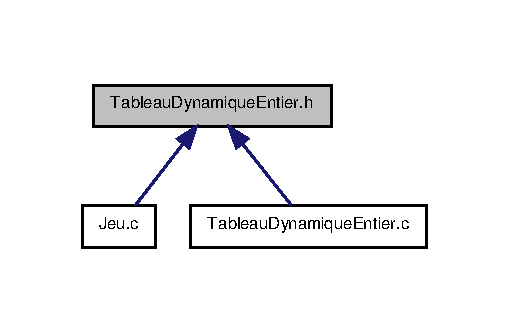
\includegraphics[width=272pt]{_tableau_dynamique_entier_8h__dep__incl}
\end{center}
\end{figure}
\subsection*{Structures de données}
\begin{DoxyCompactItemize}
\item 
struct \hyperlink{struct_tableau_dynamique_entier}{Tableau\-Dynamique\-Entier}
\end{DoxyCompactItemize}
\subsection*{Fonctions}
\begin{DoxyCompactItemize}
\item 
unsigned int \hyperlink{_tableau_dynamique_entier_8h_ab6a8726196a5f20917c43d82c7023b20}{Tab\-Dyn\-Entier\-Get\-Capacite} (const \hyperlink{struct_tableau_dynamique_entier}{Tableau\-Dynamique\-Entier} $\ast$Tab\-Dyn\-Entier)
\item 
unsigned int \hyperlink{_tableau_dynamique_entier_8h_a136e17ac632e98e56b37ec94cd375eac}{Tab\-Dyn\-Entier\-Get\-Taille\-\_\-utilisee} (const \hyperlink{struct_tableau_dynamique_entier}{Tableau\-Dynamique\-Entier} $\ast$Tab\-Dyn\-Entier)
\item 
int $\ast$ \hyperlink{_tableau_dynamique_entier_8h_a6eaf357a41e8d4fd4b4ea4ff62a6f6ed}{Tab\-Dyn\-Entier\-Get\-Ad} (const \hyperlink{struct_tableau_dynamique_entier}{Tableau\-Dynamique\-Entier} $\ast$Tab\-Dyn\-Entier)
\item 
void \hyperlink{_tableau_dynamique_entier_8h_ad954cdcf51e383884837bf7da3f46ab0}{Tab\-Dyn\-Entier\-Set\-Capacite} (\hyperlink{struct_tableau_dynamique_entier}{Tableau\-Dynamique\-Entier} $\ast$Tab\-Dyn\-Entier, unsigned int capacite)
\item 
void \hyperlink{_tableau_dynamique_entier_8h_a72608244b7a6a4af534abe48f3b7fbe2}{Tab\-Dyn\-Entier\-Set\-Taille\-\_\-utilisee} (\hyperlink{struct_tableau_dynamique_entier}{Tableau\-Dynamique\-Entier} $\ast$Tab\-Dyn\-Entier, unsigned int taille)
\item 
void \hyperlink{_tableau_dynamique_entier_8h_a943ad435f0921f55fad1004b7201819f}{Tab\-Dyn\-Entier\-Set\-Ad} (\hyperlink{struct_tableau_dynamique_entier}{Tableau\-Dynamique\-Entier} $\ast$Tab\-Dyn\-Entier, int $\ast$ad)
\item 
void \hyperlink{_tableau_dynamique_entier_8h_afe49c3b20d8e7e9075c163b5e4c6e9dc}{initialiser\-Tab\-Dyn\-Entier} (\hyperlink{struct_tableau_dynamique_entier}{Tableau\-Dynamique\-Entier} $\ast$t)
\item 
void \hyperlink{_tableau_dynamique_entier_8h_ac301681c4b3f4bce74fd9773f1da9ef6}{testament\-Tab\-Dyn\-Entier} (\hyperlink{struct_tableau_dynamique_entier}{Tableau\-Dynamique\-Entier} $\ast$t)
\item 
void \hyperlink{_tableau_dynamique_entier_8h_a0a78d0baec0923c18bd3bf611d1a0245}{affecter\-Tab\-Dyn\-Entier} (\hyperlink{struct_tableau_dynamique_entier}{Tableau\-Dynamique\-Entier} $\ast$t1, const \hyperlink{struct_tableau_dynamique_entier}{Tableau\-Dynamique\-Entier} $\ast$t2)
\item 
unsigned int \hyperlink{_tableau_dynamique_entier_8h_aff49101aadb3645be3a8abb5bfa2829c}{taille\-Utilisee\-Tab\-Dyn\-Entier} (const \hyperlink{struct_tableau_dynamique_entier}{Tableau\-Dynamique\-Entier} $\ast$t)
\item 
int \hyperlink{_tableau_dynamique_entier_8h_ad273850f79af1e74ecd32971b08fe7d8}{valeur\-Ieme\-Element\-Tab\-Dyn\-Entier} (const \hyperlink{struct_tableau_dynamique_entier}{Tableau\-Dynamique\-Entier} $\ast$t, unsigned int i)
\item 
int $\ast$ \hyperlink{_tableau_dynamique_entier_8h_ad0efdf4c23b94918071fca8711446c98}{adresse\-Ieme\-Element\-Tab\-Dyn\-Entier} (const \hyperlink{struct_tableau_dynamique_entier}{Tableau\-Dynamique\-Entier} $\ast$t, unsigned int i)
\item 
void \hyperlink{_tableau_dynamique_entier_8h_afe79a1dd09df3d0119679d87f20aec6f}{ajouter\-Element\-Tab\-Dyn\-Entier} (\hyperlink{struct_tableau_dynamique_entier}{Tableau\-Dynamique\-Entier} $\ast$t, int e)
\item 
void \hyperlink{_tableau_dynamique_entier_8h_aebe791fb2f38ce5909b196ee1f1788e1}{supprimer\-Element\-Tab\-Dyn\-Entier} (\hyperlink{struct_tableau_dynamique_entier}{Tableau\-Dynamique\-Entier} $\ast$t, int position)
\item 
void \hyperlink{_tableau_dynamique_entier_8h_a6b328364f2565029828b234d44d0bd4b}{modifier\-Valeur\-Ieme\-Element\-Tab\-Dyn\-Entier} (\hyperlink{struct_tableau_dynamique_entier}{Tableau\-Dynamique\-Entier} $\ast$t, int e, unsigned int i)
\item 
void \hyperlink{_tableau_dynamique_entier_8h_a7b813a25b809973abd95284b935b5553}{inserer\-Element\-Tab\-Dyn\-Entier} (\hyperlink{struct_tableau_dynamique_entier}{Tableau\-Dynamique\-Entier} $\ast$t, int e, unsigned int i)
\end{DoxyCompactItemize}


\subsection{Description détaillée}
\mbox{]} Module qui gère les tableaux dynamiques d'entier \begin{DoxyAuthor}{Auteur}
\{Antoine.\-C,Matthieu.\-B\} 
\end{DoxyAuthor}
\begin{DoxyVersion}{Version}
1.\-0 
\end{DoxyVersion}
\begin{DoxyDate}{Date}
19 mars 2013 
\end{DoxyDate}


Définition dans le fichier \hyperlink{_tableau_dynamique_entier_8h_source}{Tableau\-Dynamique\-Entier.\-h}.



\subsection{Documentation des fonctions}
\hypertarget{_tableau_dynamique_entier_8h_ad0efdf4c23b94918071fca8711446c98}{\index{Tableau\-Dynamique\-Entier.\-h@{Tableau\-Dynamique\-Entier.\-h}!adresse\-Ieme\-Element\-Tab\-Dyn\-Entier@{adresse\-Ieme\-Element\-Tab\-Dyn\-Entier}}
\index{adresse\-Ieme\-Element\-Tab\-Dyn\-Entier@{adresse\-Ieme\-Element\-Tab\-Dyn\-Entier}!TableauDynamiqueEntier.h@{Tableau\-Dynamique\-Entier.\-h}}
\subsubsection[{adresse\-Ieme\-Element\-Tab\-Dyn\-Entier}]{\setlength{\rightskip}{0pt plus 5cm}int$\ast$ adresse\-Ieme\-Element\-Tab\-Dyn\-Entier (
\begin{DoxyParamCaption}
\item[{const {\bf Tableau\-Dynamique\-Entier} $\ast$}]{t, }
\item[{unsigned int}]{i}
\end{DoxyParamCaption}
)}}\label{_tableau_dynamique_entier_8h_ad0efdf4c23b94918071fca8711446c98}
Precondition \-: t prealablement initialise, 0 $<$= i $<$ taille\-Utilisee(t) Resultat \-: retourne l'adresse du i+1eme Element\-T\-D de t 

Définition à la ligne 80 du fichier Tableau\-Dynamique\-Entier.\-c.

\hypertarget{_tableau_dynamique_entier_8h_a0a78d0baec0923c18bd3bf611d1a0245}{\index{Tableau\-Dynamique\-Entier.\-h@{Tableau\-Dynamique\-Entier.\-h}!affecter\-Tab\-Dyn\-Entier@{affecter\-Tab\-Dyn\-Entier}}
\index{affecter\-Tab\-Dyn\-Entier@{affecter\-Tab\-Dyn\-Entier}!TableauDynamiqueEntier.h@{Tableau\-Dynamique\-Entier.\-h}}
\subsubsection[{affecter\-Tab\-Dyn\-Entier}]{\setlength{\rightskip}{0pt plus 5cm}void affecter\-Tab\-Dyn\-Entier (
\begin{DoxyParamCaption}
\item[{{\bf Tableau\-Dynamique\-Entier} $\ast$}]{t1, }
\item[{const {\bf Tableau\-Dynamique\-Entier} $\ast$}]{t2}
\end{DoxyParamCaption}
)}}\label{_tableau_dynamique_entier_8h_a0a78d0baec0923c18bd3bf611d1a0245}
Precondition \-: t1 et t2 initialises Postcondition \-: l'ancien contenu de t1 est perdu. t1 et t2 contiennent des sequences d'Element\-T\-D identiques t1 correspond a une copie de t2, les 2 tableaux ont meme capacite, meme taille utilisee, mais sont independants) \hypertarget{_tableau_dynamique_entier_8h_afe79a1dd09df3d0119679d87f20aec6f}{\index{Tableau\-Dynamique\-Entier.\-h@{Tableau\-Dynamique\-Entier.\-h}!ajouter\-Element\-Tab\-Dyn\-Entier@{ajouter\-Element\-Tab\-Dyn\-Entier}}
\index{ajouter\-Element\-Tab\-Dyn\-Entier@{ajouter\-Element\-Tab\-Dyn\-Entier}!TableauDynamiqueEntier.h@{Tableau\-Dynamique\-Entier.\-h}}
\subsubsection[{ajouter\-Element\-Tab\-Dyn\-Entier}]{\setlength{\rightskip}{0pt plus 5cm}void ajouter\-Element\-Tab\-Dyn\-Entier (
\begin{DoxyParamCaption}
\item[{{\bf Tableau\-Dynamique\-Entier} $\ast$}]{t, }
\item[{int}]{e}
\end{DoxyParamCaption}
)}}\label{_tableau_dynamique_entier_8h_afe79a1dd09df3d0119679d87f20aec6f}
Precondition \-: t prealablement initialise Postcondition \-: L'element e est ajoute dans la premiere alveole inutilisee du tableau, la taille utilisee est incrementee de 1. Doublement de la capacite de t, si necessaire. 

Définition à la ligne 55 du fichier Tableau\-Dynamique\-Entier.\-c.

\hypertarget{_tableau_dynamique_entier_8h_afe49c3b20d8e7e9075c163b5e4c6e9dc}{\index{Tableau\-Dynamique\-Entier.\-h@{Tableau\-Dynamique\-Entier.\-h}!initialiser\-Tab\-Dyn\-Entier@{initialiser\-Tab\-Dyn\-Entier}}
\index{initialiser\-Tab\-Dyn\-Entier@{initialiser\-Tab\-Dyn\-Entier}!TableauDynamiqueEntier.h@{Tableau\-Dynamique\-Entier.\-h}}
\subsubsection[{initialiser\-Tab\-Dyn\-Entier}]{\setlength{\rightskip}{0pt plus 5cm}void initialiser\-Tab\-Dyn\-Entier (
\begin{DoxyParamCaption}
\item[{{\bf Tableau\-Dynamique\-Entier} $\ast$}]{t}
\end{DoxyParamCaption}
)}}\label{_tableau_dynamique_entier_8h_afe49c3b20d8e7e9075c163b5e4c6e9dc}
Precondition \-: t non prealablement initialise Postcondition \-: t initialise a une alveole vide (taille utilisee nulle) 

Définition à la ligne 35 du fichier Tableau\-Dynamique\-Entier.\-c.

\hypertarget{_tableau_dynamique_entier_8h_a7b813a25b809973abd95284b935b5553}{\index{Tableau\-Dynamique\-Entier.\-h@{Tableau\-Dynamique\-Entier.\-h}!inserer\-Element\-Tab\-Dyn\-Entier@{inserer\-Element\-Tab\-Dyn\-Entier}}
\index{inserer\-Element\-Tab\-Dyn\-Entier@{inserer\-Element\-Tab\-Dyn\-Entier}!TableauDynamiqueEntier.h@{Tableau\-Dynamique\-Entier.\-h}}
\subsubsection[{inserer\-Element\-Tab\-Dyn\-Entier}]{\setlength{\rightskip}{0pt plus 5cm}void inserer\-Element\-Tab\-Dyn\-Entier (
\begin{DoxyParamCaption}
\item[{{\bf Tableau\-Dynamique\-Entier} $\ast$}]{t, }
\item[{int}]{e, }
\item[{unsigned int}]{i}
\end{DoxyParamCaption}
)}}\label{_tableau_dynamique_entier_8h_a7b813a25b809973abd95284b935b5553}
Precondition \-: t prealablement initialise et 0 $<$= i $<$ taille\-Utilisee(t) Postcondition \-: e est insere en i+1eme position et taille\-Utilisee est incrementee de 1 \hypertarget{_tableau_dynamique_entier_8h_a6b328364f2565029828b234d44d0bd4b}{\index{Tableau\-Dynamique\-Entier.\-h@{Tableau\-Dynamique\-Entier.\-h}!modifier\-Valeur\-Ieme\-Element\-Tab\-Dyn\-Entier@{modifier\-Valeur\-Ieme\-Element\-Tab\-Dyn\-Entier}}
\index{modifier\-Valeur\-Ieme\-Element\-Tab\-Dyn\-Entier@{modifier\-Valeur\-Ieme\-Element\-Tab\-Dyn\-Entier}!TableauDynamiqueEntier.h@{Tableau\-Dynamique\-Entier.\-h}}
\subsubsection[{modifier\-Valeur\-Ieme\-Element\-Tab\-Dyn\-Entier}]{\setlength{\rightskip}{0pt plus 5cm}void modifier\-Valeur\-Ieme\-Element\-Tab\-Dyn\-Entier (
\begin{DoxyParamCaption}
\item[{{\bf Tableau\-Dynamique\-Entier} $\ast$}]{t, }
\item[{int}]{e, }
\item[{unsigned int}]{i}
\end{DoxyParamCaption}
)}}\label{_tableau_dynamique_entier_8h_a6b328364f2565029828b234d44d0bd4b}
Precondition \-: t prealablement initialise et 0 $<$= i $<$ taille\-Utilisee(t) Postcondition \-: le i+1eme Element\-T\-D de t vaut e 

Définition à la ligne 87 du fichier Tableau\-Dynamique\-Entier.\-c.

\hypertarget{_tableau_dynamique_entier_8h_aebe791fb2f38ce5909b196ee1f1788e1}{\index{Tableau\-Dynamique\-Entier.\-h@{Tableau\-Dynamique\-Entier.\-h}!supprimer\-Element\-Tab\-Dyn\-Entier@{supprimer\-Element\-Tab\-Dyn\-Entier}}
\index{supprimer\-Element\-Tab\-Dyn\-Entier@{supprimer\-Element\-Tab\-Dyn\-Entier}!TableauDynamiqueEntier.h@{Tableau\-Dynamique\-Entier.\-h}}
\subsubsection[{supprimer\-Element\-Tab\-Dyn\-Entier}]{\setlength{\rightskip}{0pt plus 5cm}void supprimer\-Element\-Tab\-Dyn\-Entier (
\begin{DoxyParamCaption}
\item[{{\bf Tableau\-Dynamique\-Entier} $\ast$}]{t, }
\item[{int}]{position}
\end{DoxyParamCaption}
)}}\label{_tableau_dynamique_entier_8h_aebe791fb2f38ce5909b196ee1f1788e1}
Precondition \-: t prealablement initialise et non vide Postcondition \-: la taille utilisee du tableau est decrementee de 1. Si taille\-Utilisee $<$ capacite/3, alors on divise la capacité par 2. 

Définition à la ligne 97 du fichier Tableau\-Dynamique\-Entier.\-c.

\hypertarget{_tableau_dynamique_entier_8h_a6eaf357a41e8d4fd4b4ea4ff62a6f6ed}{\index{Tableau\-Dynamique\-Entier.\-h@{Tableau\-Dynamique\-Entier.\-h}!Tab\-Dyn\-Entier\-Get\-Ad@{Tab\-Dyn\-Entier\-Get\-Ad}}
\index{Tab\-Dyn\-Entier\-Get\-Ad@{Tab\-Dyn\-Entier\-Get\-Ad}!TableauDynamiqueEntier.h@{Tableau\-Dynamique\-Entier.\-h}}
\subsubsection[{Tab\-Dyn\-Entier\-Get\-Ad}]{\setlength{\rightskip}{0pt plus 5cm}int$\ast$ Tab\-Dyn\-Entier\-Get\-Ad (
\begin{DoxyParamCaption}
\item[{const {\bf Tableau\-Dynamique\-Entier} $\ast$}]{Tab\-Dyn\-Entier}
\end{DoxyParamCaption}
)}}\label{_tableau_dynamique_entier_8h_a6eaf357a41e8d4fd4b4ea4ff62a6f6ed}
assesseur de ad 

Définition à la ligne 18 du fichier Tableau\-Dynamique\-Entier.\-c.

\hypertarget{_tableau_dynamique_entier_8h_ab6a8726196a5f20917c43d82c7023b20}{\index{Tableau\-Dynamique\-Entier.\-h@{Tableau\-Dynamique\-Entier.\-h}!Tab\-Dyn\-Entier\-Get\-Capacite@{Tab\-Dyn\-Entier\-Get\-Capacite}}
\index{Tab\-Dyn\-Entier\-Get\-Capacite@{Tab\-Dyn\-Entier\-Get\-Capacite}!TableauDynamiqueEntier.h@{Tableau\-Dynamique\-Entier.\-h}}
\subsubsection[{Tab\-Dyn\-Entier\-Get\-Capacite}]{\setlength{\rightskip}{0pt plus 5cm}unsigned int Tab\-Dyn\-Entier\-Get\-Capacite (
\begin{DoxyParamCaption}
\item[{const {\bf Tableau\-Dynamique\-Entier} $\ast$}]{Tab\-Dyn\-Entier}
\end{DoxyParamCaption}
)}}\label{_tableau_dynamique_entier_8h_ab6a8726196a5f20917c43d82c7023b20}
assesseur de capacite 

Définition à la ligne 12 du fichier Tableau\-Dynamique\-Entier.\-c.

\hypertarget{_tableau_dynamique_entier_8h_a136e17ac632e98e56b37ec94cd375eac}{\index{Tableau\-Dynamique\-Entier.\-h@{Tableau\-Dynamique\-Entier.\-h}!Tab\-Dyn\-Entier\-Get\-Taille\-\_\-utilisee@{Tab\-Dyn\-Entier\-Get\-Taille\-\_\-utilisee}}
\index{Tab\-Dyn\-Entier\-Get\-Taille\-\_\-utilisee@{Tab\-Dyn\-Entier\-Get\-Taille\-\_\-utilisee}!TableauDynamiqueEntier.h@{Tableau\-Dynamique\-Entier.\-h}}
\subsubsection[{Tab\-Dyn\-Entier\-Get\-Taille\-\_\-utilisee}]{\setlength{\rightskip}{0pt plus 5cm}unsigned int Tab\-Dyn\-Entier\-Get\-Taille\-\_\-utilisee (
\begin{DoxyParamCaption}
\item[{const {\bf Tableau\-Dynamique\-Entier} $\ast$}]{Tab\-Dyn\-Entier}
\end{DoxyParamCaption}
)}}\label{_tableau_dynamique_entier_8h_a136e17ac632e98e56b37ec94cd375eac}
assesseur de taille\-\_\-utilisee 

Définition à la ligne 15 du fichier Tableau\-Dynamique\-Entier.\-c.

\hypertarget{_tableau_dynamique_entier_8h_a943ad435f0921f55fad1004b7201819f}{\index{Tableau\-Dynamique\-Entier.\-h@{Tableau\-Dynamique\-Entier.\-h}!Tab\-Dyn\-Entier\-Set\-Ad@{Tab\-Dyn\-Entier\-Set\-Ad}}
\index{Tab\-Dyn\-Entier\-Set\-Ad@{Tab\-Dyn\-Entier\-Set\-Ad}!TableauDynamiqueEntier.h@{Tableau\-Dynamique\-Entier.\-h}}
\subsubsection[{Tab\-Dyn\-Entier\-Set\-Ad}]{\setlength{\rightskip}{0pt plus 5cm}void Tab\-Dyn\-Entier\-Set\-Ad (
\begin{DoxyParamCaption}
\item[{{\bf Tableau\-Dynamique\-Entier} $\ast$}]{Tab\-Dyn\-Entier, }
\item[{int $\ast$}]{ad}
\end{DoxyParamCaption}
)}}\label{_tableau_dynamique_entier_8h_a943ad435f0921f55fad1004b7201819f}
mutateur de ad 

Définition à la ligne 28 du fichier Tableau\-Dynamique\-Entier.\-c.

\hypertarget{_tableau_dynamique_entier_8h_ad954cdcf51e383884837bf7da3f46ab0}{\index{Tableau\-Dynamique\-Entier.\-h@{Tableau\-Dynamique\-Entier.\-h}!Tab\-Dyn\-Entier\-Set\-Capacite@{Tab\-Dyn\-Entier\-Set\-Capacite}}
\index{Tab\-Dyn\-Entier\-Set\-Capacite@{Tab\-Dyn\-Entier\-Set\-Capacite}!TableauDynamiqueEntier.h@{Tableau\-Dynamique\-Entier.\-h}}
\subsubsection[{Tab\-Dyn\-Entier\-Set\-Capacite}]{\setlength{\rightskip}{0pt plus 5cm}void Tab\-Dyn\-Entier\-Set\-Capacite (
\begin{DoxyParamCaption}
\item[{{\bf Tableau\-Dynamique\-Entier} $\ast$}]{Tab\-Dyn\-Entier, }
\item[{unsigned int}]{capacite}
\end{DoxyParamCaption}
)}}\label{_tableau_dynamique_entier_8h_ad954cdcf51e383884837bf7da3f46ab0}
mutateur de capacite 

Définition à la ligne 22 du fichier Tableau\-Dynamique\-Entier.\-c.

\hypertarget{_tableau_dynamique_entier_8h_a72608244b7a6a4af534abe48f3b7fbe2}{\index{Tableau\-Dynamique\-Entier.\-h@{Tableau\-Dynamique\-Entier.\-h}!Tab\-Dyn\-Entier\-Set\-Taille\-\_\-utilisee@{Tab\-Dyn\-Entier\-Set\-Taille\-\_\-utilisee}}
\index{Tab\-Dyn\-Entier\-Set\-Taille\-\_\-utilisee@{Tab\-Dyn\-Entier\-Set\-Taille\-\_\-utilisee}!TableauDynamiqueEntier.h@{Tableau\-Dynamique\-Entier.\-h}}
\subsubsection[{Tab\-Dyn\-Entier\-Set\-Taille\-\_\-utilisee}]{\setlength{\rightskip}{0pt plus 5cm}void Tab\-Dyn\-Entier\-Set\-Taille\-\_\-utilisee (
\begin{DoxyParamCaption}
\item[{{\bf Tableau\-Dynamique\-Entier} $\ast$}]{Tab\-Dyn\-Entier, }
\item[{unsigned int}]{taille}
\end{DoxyParamCaption}
)}}\label{_tableau_dynamique_entier_8h_a72608244b7a6a4af534abe48f3b7fbe2}
mutateur de taille\-\_\-utilisee 

Définition à la ligne 25 du fichier Tableau\-Dynamique\-Entier.\-c.

\hypertarget{_tableau_dynamique_entier_8h_aff49101aadb3645be3a8abb5bfa2829c}{\index{Tableau\-Dynamique\-Entier.\-h@{Tableau\-Dynamique\-Entier.\-h}!taille\-Utilisee\-Tab\-Dyn\-Entier@{taille\-Utilisee\-Tab\-Dyn\-Entier}}
\index{taille\-Utilisee\-Tab\-Dyn\-Entier@{taille\-Utilisee\-Tab\-Dyn\-Entier}!TableauDynamiqueEntier.h@{Tableau\-Dynamique\-Entier.\-h}}
\subsubsection[{taille\-Utilisee\-Tab\-Dyn\-Entier}]{\setlength{\rightskip}{0pt plus 5cm}unsigned int taille\-Utilisee\-Tab\-Dyn\-Entier (
\begin{DoxyParamCaption}
\item[{const {\bf Tableau\-Dynamique\-Entier} $\ast$}]{t}
\end{DoxyParamCaption}
)}}\label{_tableau_dynamique_entier_8h_aff49101aadb3645be3a8abb5bfa2829c}
Precondition \-: t prealablement initialise Resultat \-: nombre d'Element\-T\-Ds stockes dans t \hypertarget{_tableau_dynamique_entier_8h_ac301681c4b3f4bce74fd9773f1da9ef6}{\index{Tableau\-Dynamique\-Entier.\-h@{Tableau\-Dynamique\-Entier.\-h}!testament\-Tab\-Dyn\-Entier@{testament\-Tab\-Dyn\-Entier}}
\index{testament\-Tab\-Dyn\-Entier@{testament\-Tab\-Dyn\-Entier}!TableauDynamiqueEntier.h@{Tableau\-Dynamique\-Entier.\-h}}
\subsubsection[{testament\-Tab\-Dyn\-Entier}]{\setlength{\rightskip}{0pt plus 5cm}void testament\-Tab\-Dyn\-Entier (
\begin{DoxyParamCaption}
\item[{{\bf Tableau\-Dynamique\-Entier} $\ast$}]{t}
\end{DoxyParamCaption}
)}}\label{_tableau_dynamique_entier_8h_ac301681c4b3f4bce74fd9773f1da9ef6}
\begin{DoxyVerb}Precondition : t prealablement initialise
\end{DoxyVerb}
 Postcondition \-: t pret a disparaitre. La memoire allouee dynamiquement est liberee. On ne pourra plus appeler les sous-\/programmes qui necessitent que t soit initialise. 

Définition à la ligne 43 du fichier Tableau\-Dynamique\-Entier.\-c.

\hypertarget{_tableau_dynamique_entier_8h_ad273850f79af1e74ecd32971b08fe7d8}{\index{Tableau\-Dynamique\-Entier.\-h@{Tableau\-Dynamique\-Entier.\-h}!valeur\-Ieme\-Element\-Tab\-Dyn\-Entier@{valeur\-Ieme\-Element\-Tab\-Dyn\-Entier}}
\index{valeur\-Ieme\-Element\-Tab\-Dyn\-Entier@{valeur\-Ieme\-Element\-Tab\-Dyn\-Entier}!TableauDynamiqueEntier.h@{Tableau\-Dynamique\-Entier.\-h}}
\subsubsection[{valeur\-Ieme\-Element\-Tab\-Dyn\-Entier}]{\setlength{\rightskip}{0pt plus 5cm}int valeur\-Ieme\-Element\-Tab\-Dyn\-Entier (
\begin{DoxyParamCaption}
\item[{const {\bf Tableau\-Dynamique\-Entier} $\ast$}]{t, }
\item[{unsigned int}]{i}
\end{DoxyParamCaption}
)}}\label{_tableau_dynamique_entier_8h_ad273850f79af1e74ecd32971b08fe7d8}
Precondition \-: t prealablement initialise, 0 $<$= i $<$ taille\-Utilisee(t) Resultat \-: retourne le i+1eme Element\-T\-D de t 

Définition à la ligne 75 du fichier Tableau\-Dynamique\-Entier.\-c.


\hypertarget{_tableau_dynamique_mur_8c}{\section{Référence du fichier Tableau\-Dynamique\-Mur.\-c}
\label{_tableau_dynamique_mur_8c}\index{Tableau\-Dynamique\-Mur.\-c@{Tableau\-Dynamique\-Mur.\-c}}
}
{\ttfamily \#include \char`\"{}Tableau\-Dynamique\-Mur.\-h\char`\"{}}\\*
{\ttfamily \#include $<$stdio.\-h$>$}\\*
{\ttfamily \#include \char`\"{}Mur.\-h\char`\"{}}\\*
{\ttfamily \#include $<$stdlib.\-h$>$}\\*
Graphe des dépendances par inclusion de Tableau\-Dynamique\-Mur.\-c\-:\nopagebreak
\begin{figure}[H]
\begin{center}
\leavevmode
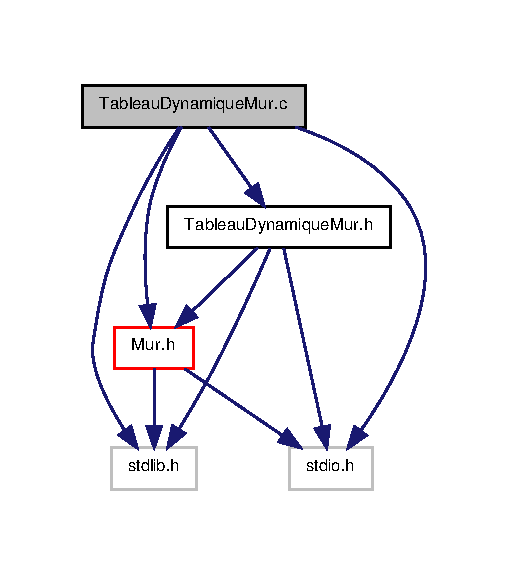
\includegraphics[width=275pt]{_tableau_dynamique_mur_8c__incl}
\end{center}
\end{figure}
\subsection*{Fonctions}
\begin{DoxyCompactItemize}
\item 
unsigned int \hyperlink{_tableau_dynamique_mur_8c_a9d8993673abb44cb220526fc555b97e6}{Tab\-Dyn\-Mur\-Get\-Capacite} (const \hyperlink{struct_tableau_dynamique_mur}{Tableau\-Dynamique\-Mur} $\ast$Tab\-Dyn\-Mur)
\item 
unsigned int \hyperlink{_tableau_dynamique_mur_8c_aa4cccc53a5d36a7df78f86d878a89d96}{Tab\-Dyn\-Mur\-Get\-Taille\-\_\-utilisee} (const \hyperlink{struct_tableau_dynamique_mur}{Tableau\-Dynamique\-Mur} $\ast$Tab\-Dyn\-Mur)
\item 
\hyperlink{struct_mur}{Mur} $\ast$ \hyperlink{_tableau_dynamique_mur_8c_adcadf52764b8e0f32e4844495e3a6724}{Tab\-Dyn\-Mur\-Get\-Ad} (const \hyperlink{struct_tableau_dynamique_mur}{Tableau\-Dynamique\-Mur} $\ast$Tab\-Dyn\-Mur)
\item 
void \hyperlink{_tableau_dynamique_mur_8c_ac0e544e5c2190470f1c888403dd5e75b}{Tab\-Dyn\-Mur\-Set\-Capacite} (\hyperlink{struct_tableau_dynamique_mur}{Tableau\-Dynamique\-Mur} $\ast$Tab\-Dyn\-Mur, unsigned int capacite)
\item 
void \hyperlink{_tableau_dynamique_mur_8c_a8cab81dcce42531992bc233a0a0c91d1}{Tab\-Dyn\-Mur\-Set\-Taille\-\_\-utilisee} (\hyperlink{struct_tableau_dynamique_mur}{Tableau\-Dynamique\-Mur} $\ast$Tab\-Dyn\-Mur, unsigned int taille)
\item 
void \hyperlink{_tableau_dynamique_mur_8c_a247f1e88f472662f5a794384760ca2bc}{Tab\-Dyn\-Mur\-Set\-Ad} (\hyperlink{struct_tableau_dynamique_mur}{Tableau\-Dynamique\-Mur} $\ast$Tab\-Dyn\-Mur, \hyperlink{struct_mur}{Mur} $\ast$ad)
\item 
void \hyperlink{_tableau_dynamique_mur_8c_a677de455353d6c7d8e49e9d8b765f085}{initialiser\-Tab\-Dyn\-Mur} (\hyperlink{struct_tableau_dynamique_mur}{Tableau\-Dynamique\-Mur} $\ast$t)
\item 
void \hyperlink{_tableau_dynamique_mur_8c_ad33a7af085e713d488c62e232464c025}{testament\-Tab\-Dyn\-Mur} (\hyperlink{struct_tableau_dynamique_mur}{Tableau\-Dynamique\-Mur} $\ast$t)
\item 
void \hyperlink{_tableau_dynamique_mur_8c_a76e95156313a16c5956402a00faac297}{ajouter\-Element\-Tab\-Dyn\-Mur} (\hyperlink{struct_tableau_dynamique_mur}{Tableau\-Dynamique\-Mur} $\ast$t, \hyperlink{struct_mur}{Mur} e)
\item 
\hyperlink{struct_mur}{Mur} \hyperlink{_tableau_dynamique_mur_8c_a4b1cf99f3ab429c58cc4f87134dfb146}{valeur\-Ieme\-Element\-Tab\-Dyn\-Mur} (const \hyperlink{struct_tableau_dynamique_mur}{Tableau\-Dynamique\-Mur} $\ast$t, unsigned int i)
\item 
\hyperlink{struct_mur}{Mur} $\ast$ \hyperlink{_tableau_dynamique_mur_8c_a91faee7eb572734cef6f3b81b9793352}{adresse\-Ieme\-Element\-Tab\-Dyn\-Mur} (const \hyperlink{struct_tableau_dynamique_mur}{Tableau\-Dynamique\-Mur} $\ast$t, unsigned int i)
\item 
void \hyperlink{_tableau_dynamique_mur_8c_ac9e49d24407d337a101c5186534ab0d0}{modifier\-Valeur\-Ieme\-Element\-Tab\-Dyn\-Mur} (\hyperlink{struct_tableau_dynamique_mur}{Tableau\-Dynamique\-Mur} $\ast$t, \hyperlink{struct_mur}{Mur} e, unsigned int i)
\item 
void \hyperlink{_tableau_dynamique_mur_8c_ac1f6eb509e569f5887171ec6add66d30}{supprimer\-Element\-Tab\-Dyn\-Mur} (\hyperlink{struct_tableau_dynamique_mur}{Tableau\-Dynamique\-Mur} $\ast$t, int position)
\end{DoxyCompactItemize}


\subsection{Description détaillée}
\mbox{]} Module qui gère les tableaux dynamiques des Murs \begin{DoxyAuthor}{Auteur}
\{Antoine.\-C,Matthieu.\-B\} 
\end{DoxyAuthor}
\begin{DoxyVersion}{Version}
1.\-0 
\end{DoxyVersion}
\begin{DoxyDate}{Date}
19 mars 2013 
\end{DoxyDate}


Définition dans le fichier \hyperlink{_tableau_dynamique_mur_8c_source}{Tableau\-Dynamique\-Mur.\-c}.



\subsection{Documentation des fonctions}
\hypertarget{_tableau_dynamique_mur_8c_a91faee7eb572734cef6f3b81b9793352}{\index{Tableau\-Dynamique\-Mur.\-c@{Tableau\-Dynamique\-Mur.\-c}!adresse\-Ieme\-Element\-Tab\-Dyn\-Mur@{adresse\-Ieme\-Element\-Tab\-Dyn\-Mur}}
\index{adresse\-Ieme\-Element\-Tab\-Dyn\-Mur@{adresse\-Ieme\-Element\-Tab\-Dyn\-Mur}!TableauDynamiqueMur.c@{Tableau\-Dynamique\-Mur.\-c}}
\subsubsection[{adresse\-Ieme\-Element\-Tab\-Dyn\-Mur}]{\setlength{\rightskip}{0pt plus 5cm}{\bf Mur}$\ast$ adresse\-Ieme\-Element\-Tab\-Dyn\-Mur (
\begin{DoxyParamCaption}
\item[{const {\bf Tableau\-Dynamique\-Mur} $\ast$}]{t, }
\item[{unsigned int}]{i}
\end{DoxyParamCaption}
)}}\label{_tableau_dynamique_mur_8c_a91faee7eb572734cef6f3b81b9793352}
Precondition \-: t prealablement initialise, 0 $<$= i $<$ taille\-Utilisee(t) Resultat \-: retourne l'adresse du i+1eme Element\-T\-D de t 

Définition à la ligne 82 du fichier Tableau\-Dynamique\-Mur.\-c.

\hypertarget{_tableau_dynamique_mur_8c_a76e95156313a16c5956402a00faac297}{\index{Tableau\-Dynamique\-Mur.\-c@{Tableau\-Dynamique\-Mur.\-c}!ajouter\-Element\-Tab\-Dyn\-Mur@{ajouter\-Element\-Tab\-Dyn\-Mur}}
\index{ajouter\-Element\-Tab\-Dyn\-Mur@{ajouter\-Element\-Tab\-Dyn\-Mur}!TableauDynamiqueMur.c@{Tableau\-Dynamique\-Mur.\-c}}
\subsubsection[{ajouter\-Element\-Tab\-Dyn\-Mur}]{\setlength{\rightskip}{0pt plus 5cm}void ajouter\-Element\-Tab\-Dyn\-Mur (
\begin{DoxyParamCaption}
\item[{{\bf Tableau\-Dynamique\-Mur} $\ast$}]{t, }
\item[{{\bf Mur}}]{e}
\end{DoxyParamCaption}
)}}\label{_tableau_dynamique_mur_8c_a76e95156313a16c5956402a00faac297}
Precondition \-: t prealablement initialise Postcondition \-: L'element e est ajoute dans la premiere alveole inutilisee du tableau, la taille utilisee est incrementee de 1. Doublement de la capacite de t, si necessaire. 

Définition à la ligne 57 du fichier Tableau\-Dynamique\-Mur.\-c.

\hypertarget{_tableau_dynamique_mur_8c_a677de455353d6c7d8e49e9d8b765f085}{\index{Tableau\-Dynamique\-Mur.\-c@{Tableau\-Dynamique\-Mur.\-c}!initialiser\-Tab\-Dyn\-Mur@{initialiser\-Tab\-Dyn\-Mur}}
\index{initialiser\-Tab\-Dyn\-Mur@{initialiser\-Tab\-Dyn\-Mur}!TableauDynamiqueMur.c@{Tableau\-Dynamique\-Mur.\-c}}
\subsubsection[{initialiser\-Tab\-Dyn\-Mur}]{\setlength{\rightskip}{0pt plus 5cm}void initialiser\-Tab\-Dyn\-Mur (
\begin{DoxyParamCaption}
\item[{{\bf Tableau\-Dynamique\-Mur} $\ast$}]{t}
\end{DoxyParamCaption}
)}}\label{_tableau_dynamique_mur_8c_a677de455353d6c7d8e49e9d8b765f085}
Precondition \-: t non prealablement initialise Postcondition \-: t initialise a une alveole vide (taille utilisee nulle) 

Définition à la ligne 37 du fichier Tableau\-Dynamique\-Mur.\-c.

\hypertarget{_tableau_dynamique_mur_8c_ac9e49d24407d337a101c5186534ab0d0}{\index{Tableau\-Dynamique\-Mur.\-c@{Tableau\-Dynamique\-Mur.\-c}!modifier\-Valeur\-Ieme\-Element\-Tab\-Dyn\-Mur@{modifier\-Valeur\-Ieme\-Element\-Tab\-Dyn\-Mur}}
\index{modifier\-Valeur\-Ieme\-Element\-Tab\-Dyn\-Mur@{modifier\-Valeur\-Ieme\-Element\-Tab\-Dyn\-Mur}!TableauDynamiqueMur.c@{Tableau\-Dynamique\-Mur.\-c}}
\subsubsection[{modifier\-Valeur\-Ieme\-Element\-Tab\-Dyn\-Mur}]{\setlength{\rightskip}{0pt plus 5cm}void modifier\-Valeur\-Ieme\-Element\-Tab\-Dyn\-Mur (
\begin{DoxyParamCaption}
\item[{{\bf Tableau\-Dynamique\-Mur} $\ast$}]{t, }
\item[{{\bf Mur}}]{e, }
\item[{unsigned int}]{i}
\end{DoxyParamCaption}
)}}\label{_tableau_dynamique_mur_8c_ac9e49d24407d337a101c5186534ab0d0}
Precondition \-: t prealablement initialise et 0 $<$= i $<$ taille\-Utilisee(t) Postcondition \-: le i+1eme Element\-T\-D de t vaut e 

Définition à la ligne 89 du fichier Tableau\-Dynamique\-Mur.\-c.

\hypertarget{_tableau_dynamique_mur_8c_ac1f6eb509e569f5887171ec6add66d30}{\index{Tableau\-Dynamique\-Mur.\-c@{Tableau\-Dynamique\-Mur.\-c}!supprimer\-Element\-Tab\-Dyn\-Mur@{supprimer\-Element\-Tab\-Dyn\-Mur}}
\index{supprimer\-Element\-Tab\-Dyn\-Mur@{supprimer\-Element\-Tab\-Dyn\-Mur}!TableauDynamiqueMur.c@{Tableau\-Dynamique\-Mur.\-c}}
\subsubsection[{supprimer\-Element\-Tab\-Dyn\-Mur}]{\setlength{\rightskip}{0pt plus 5cm}void supprimer\-Element\-Tab\-Dyn\-Mur (
\begin{DoxyParamCaption}
\item[{{\bf Tableau\-Dynamique\-Mur} $\ast$}]{t, }
\item[{int}]{position}
\end{DoxyParamCaption}
)}}\label{_tableau_dynamique_mur_8c_ac1f6eb509e569f5887171ec6add66d30}
Precondition \-: t prealablement initialise et non vide Postcondition \-: la taille utilisee du tableau est decrementee de 1. Si taille\-Utilisee $<$ capacite/3, alors on divise la capacité par 2. 

Définition à la ligne 99 du fichier Tableau\-Dynamique\-Mur.\-c.

\hypertarget{_tableau_dynamique_mur_8c_adcadf52764b8e0f32e4844495e3a6724}{\index{Tableau\-Dynamique\-Mur.\-c@{Tableau\-Dynamique\-Mur.\-c}!Tab\-Dyn\-Mur\-Get\-Ad@{Tab\-Dyn\-Mur\-Get\-Ad}}
\index{Tab\-Dyn\-Mur\-Get\-Ad@{Tab\-Dyn\-Mur\-Get\-Ad}!TableauDynamiqueMur.c@{Tableau\-Dynamique\-Mur.\-c}}
\subsubsection[{Tab\-Dyn\-Mur\-Get\-Ad}]{\setlength{\rightskip}{0pt plus 5cm}{\bf Mur}$\ast$ Tab\-Dyn\-Mur\-Get\-Ad (
\begin{DoxyParamCaption}
\item[{const {\bf Tableau\-Dynamique\-Mur} $\ast$}]{Tab\-Dyn\-Mur}
\end{DoxyParamCaption}
)}}\label{_tableau_dynamique_mur_8c_adcadf52764b8e0f32e4844495e3a6724}
assesseur de ad 

Définition à la ligne 20 du fichier Tableau\-Dynamique\-Mur.\-c.

\hypertarget{_tableau_dynamique_mur_8c_a9d8993673abb44cb220526fc555b97e6}{\index{Tableau\-Dynamique\-Mur.\-c@{Tableau\-Dynamique\-Mur.\-c}!Tab\-Dyn\-Mur\-Get\-Capacite@{Tab\-Dyn\-Mur\-Get\-Capacite}}
\index{Tab\-Dyn\-Mur\-Get\-Capacite@{Tab\-Dyn\-Mur\-Get\-Capacite}!TableauDynamiqueMur.c@{Tableau\-Dynamique\-Mur.\-c}}
\subsubsection[{Tab\-Dyn\-Mur\-Get\-Capacite}]{\setlength{\rightskip}{0pt plus 5cm}unsigned int Tab\-Dyn\-Mur\-Get\-Capacite (
\begin{DoxyParamCaption}
\item[{const {\bf Tableau\-Dynamique\-Mur} $\ast$}]{Tab\-Dyn\-Mur}
\end{DoxyParamCaption}
)}}\label{_tableau_dynamique_mur_8c_a9d8993673abb44cb220526fc555b97e6}
assesseur de capacite 

Définition à la ligne 14 du fichier Tableau\-Dynamique\-Mur.\-c.

\hypertarget{_tableau_dynamique_mur_8c_aa4cccc53a5d36a7df78f86d878a89d96}{\index{Tableau\-Dynamique\-Mur.\-c@{Tableau\-Dynamique\-Mur.\-c}!Tab\-Dyn\-Mur\-Get\-Taille\-\_\-utilisee@{Tab\-Dyn\-Mur\-Get\-Taille\-\_\-utilisee}}
\index{Tab\-Dyn\-Mur\-Get\-Taille\-\_\-utilisee@{Tab\-Dyn\-Mur\-Get\-Taille\-\_\-utilisee}!TableauDynamiqueMur.c@{Tableau\-Dynamique\-Mur.\-c}}
\subsubsection[{Tab\-Dyn\-Mur\-Get\-Taille\-\_\-utilisee}]{\setlength{\rightskip}{0pt plus 5cm}unsigned int Tab\-Dyn\-Mur\-Get\-Taille\-\_\-utilisee (
\begin{DoxyParamCaption}
\item[{const {\bf Tableau\-Dynamique\-Mur} $\ast$}]{Tab\-Dyn\-Mur}
\end{DoxyParamCaption}
)}}\label{_tableau_dynamique_mur_8c_aa4cccc53a5d36a7df78f86d878a89d96}
assesseur de taille\-\_\-utilisee 

Définition à la ligne 17 du fichier Tableau\-Dynamique\-Mur.\-c.

\hypertarget{_tableau_dynamique_mur_8c_a247f1e88f472662f5a794384760ca2bc}{\index{Tableau\-Dynamique\-Mur.\-c@{Tableau\-Dynamique\-Mur.\-c}!Tab\-Dyn\-Mur\-Set\-Ad@{Tab\-Dyn\-Mur\-Set\-Ad}}
\index{Tab\-Dyn\-Mur\-Set\-Ad@{Tab\-Dyn\-Mur\-Set\-Ad}!TableauDynamiqueMur.c@{Tableau\-Dynamique\-Mur.\-c}}
\subsubsection[{Tab\-Dyn\-Mur\-Set\-Ad}]{\setlength{\rightskip}{0pt plus 5cm}void Tab\-Dyn\-Mur\-Set\-Ad (
\begin{DoxyParamCaption}
\item[{{\bf Tableau\-Dynamique\-Mur} $\ast$}]{Tab\-Dyn\-Mur, }
\item[{{\bf Mur} $\ast$}]{ad}
\end{DoxyParamCaption}
)}}\label{_tableau_dynamique_mur_8c_a247f1e88f472662f5a794384760ca2bc}
mutateur de ad 

Définition à la ligne 30 du fichier Tableau\-Dynamique\-Mur.\-c.

\hypertarget{_tableau_dynamique_mur_8c_ac0e544e5c2190470f1c888403dd5e75b}{\index{Tableau\-Dynamique\-Mur.\-c@{Tableau\-Dynamique\-Mur.\-c}!Tab\-Dyn\-Mur\-Set\-Capacite@{Tab\-Dyn\-Mur\-Set\-Capacite}}
\index{Tab\-Dyn\-Mur\-Set\-Capacite@{Tab\-Dyn\-Mur\-Set\-Capacite}!TableauDynamiqueMur.c@{Tableau\-Dynamique\-Mur.\-c}}
\subsubsection[{Tab\-Dyn\-Mur\-Set\-Capacite}]{\setlength{\rightskip}{0pt plus 5cm}void Tab\-Dyn\-Mur\-Set\-Capacite (
\begin{DoxyParamCaption}
\item[{{\bf Tableau\-Dynamique\-Mur} $\ast$}]{Tab\-Dyn\-Mur, }
\item[{unsigned int}]{capacite}
\end{DoxyParamCaption}
)}}\label{_tableau_dynamique_mur_8c_ac0e544e5c2190470f1c888403dd5e75b}
mutateur de capacite 

Définition à la ligne 24 du fichier Tableau\-Dynamique\-Mur.\-c.

\hypertarget{_tableau_dynamique_mur_8c_a8cab81dcce42531992bc233a0a0c91d1}{\index{Tableau\-Dynamique\-Mur.\-c@{Tableau\-Dynamique\-Mur.\-c}!Tab\-Dyn\-Mur\-Set\-Taille\-\_\-utilisee@{Tab\-Dyn\-Mur\-Set\-Taille\-\_\-utilisee}}
\index{Tab\-Dyn\-Mur\-Set\-Taille\-\_\-utilisee@{Tab\-Dyn\-Mur\-Set\-Taille\-\_\-utilisee}!TableauDynamiqueMur.c@{Tableau\-Dynamique\-Mur.\-c}}
\subsubsection[{Tab\-Dyn\-Mur\-Set\-Taille\-\_\-utilisee}]{\setlength{\rightskip}{0pt plus 5cm}void Tab\-Dyn\-Mur\-Set\-Taille\-\_\-utilisee (
\begin{DoxyParamCaption}
\item[{{\bf Tableau\-Dynamique\-Mur} $\ast$}]{Tab\-Dyn\-Mur, }
\item[{unsigned int}]{taille}
\end{DoxyParamCaption}
)}}\label{_tableau_dynamique_mur_8c_a8cab81dcce42531992bc233a0a0c91d1}
mutateur de taille\-\_\-utilisee 

Définition à la ligne 27 du fichier Tableau\-Dynamique\-Mur.\-c.

\hypertarget{_tableau_dynamique_mur_8c_ad33a7af085e713d488c62e232464c025}{\index{Tableau\-Dynamique\-Mur.\-c@{Tableau\-Dynamique\-Mur.\-c}!testament\-Tab\-Dyn\-Mur@{testament\-Tab\-Dyn\-Mur}}
\index{testament\-Tab\-Dyn\-Mur@{testament\-Tab\-Dyn\-Mur}!TableauDynamiqueMur.c@{Tableau\-Dynamique\-Mur.\-c}}
\subsubsection[{testament\-Tab\-Dyn\-Mur}]{\setlength{\rightskip}{0pt plus 5cm}void testament\-Tab\-Dyn\-Mur (
\begin{DoxyParamCaption}
\item[{{\bf Tableau\-Dynamique\-Mur} $\ast$}]{t}
\end{DoxyParamCaption}
)}}\label{_tableau_dynamique_mur_8c_ad33a7af085e713d488c62e232464c025}
\begin{DoxyVerb}Precondition : t prealablement initialise
\end{DoxyVerb}
 Postcondition \-: t pret a disparaitre. La memoire allouee dynamiquement est liberee. On ne pourra plus appeler les sous-\/programmes qui necessitent que t soit initialise. 

Définition à la ligne 45 du fichier Tableau\-Dynamique\-Mur.\-c.

\hypertarget{_tableau_dynamique_mur_8c_a4b1cf99f3ab429c58cc4f87134dfb146}{\index{Tableau\-Dynamique\-Mur.\-c@{Tableau\-Dynamique\-Mur.\-c}!valeur\-Ieme\-Element\-Tab\-Dyn\-Mur@{valeur\-Ieme\-Element\-Tab\-Dyn\-Mur}}
\index{valeur\-Ieme\-Element\-Tab\-Dyn\-Mur@{valeur\-Ieme\-Element\-Tab\-Dyn\-Mur}!TableauDynamiqueMur.c@{Tableau\-Dynamique\-Mur.\-c}}
\subsubsection[{valeur\-Ieme\-Element\-Tab\-Dyn\-Mur}]{\setlength{\rightskip}{0pt plus 5cm}{\bf Mur} valeur\-Ieme\-Element\-Tab\-Dyn\-Mur (
\begin{DoxyParamCaption}
\item[{const {\bf Tableau\-Dynamique\-Mur} $\ast$}]{t, }
\item[{unsigned int}]{i}
\end{DoxyParamCaption}
)}}\label{_tableau_dynamique_mur_8c_a4b1cf99f3ab429c58cc4f87134dfb146}
Precondition \-: t prealablement initialise, 0 $<$= i $<$ taille\-Utilisee(t) Resultat \-: retourne le i+1eme Element\-T\-D de t 

Définition à la ligne 77 du fichier Tableau\-Dynamique\-Mur.\-c.


\hypertarget{_tableau_dynamique_mur_8h}{\section{Référence du fichier Tableau\-Dynamique\-Mur.\-h}
\label{_tableau_dynamique_mur_8h}\index{Tableau\-Dynamique\-Mur.\-h@{Tableau\-Dynamique\-Mur.\-h}}
}
{\ttfamily \#include \char`\"{}Mur.\-h\char`\"{}}\\*
{\ttfamily \#include $<$stdio.\-h$>$}\\*
{\ttfamily \#include $<$stdlib.\-h$>$}\\*
Graphe des dépendances par inclusion de Tableau\-Dynamique\-Mur.\-h\-:\nopagebreak
\begin{figure}[H]
\begin{center}
\leavevmode
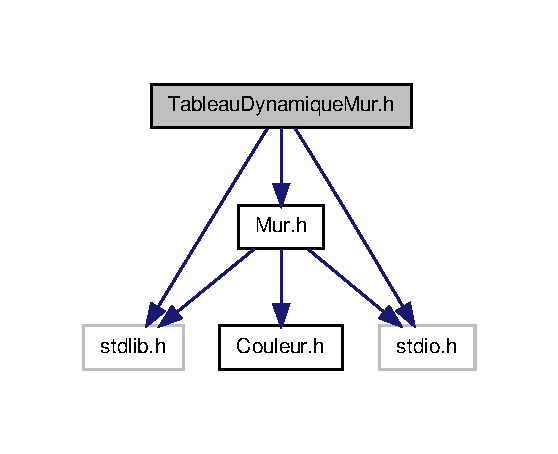
\includegraphics[width=268pt]{_tableau_dynamique_mur_8h__incl}
\end{center}
\end{figure}
Ce graphe montre quels fichiers incluent directement ou indirectement ce fichier \-:\nopagebreak
\begin{figure}[H]
\begin{center}
\leavevmode
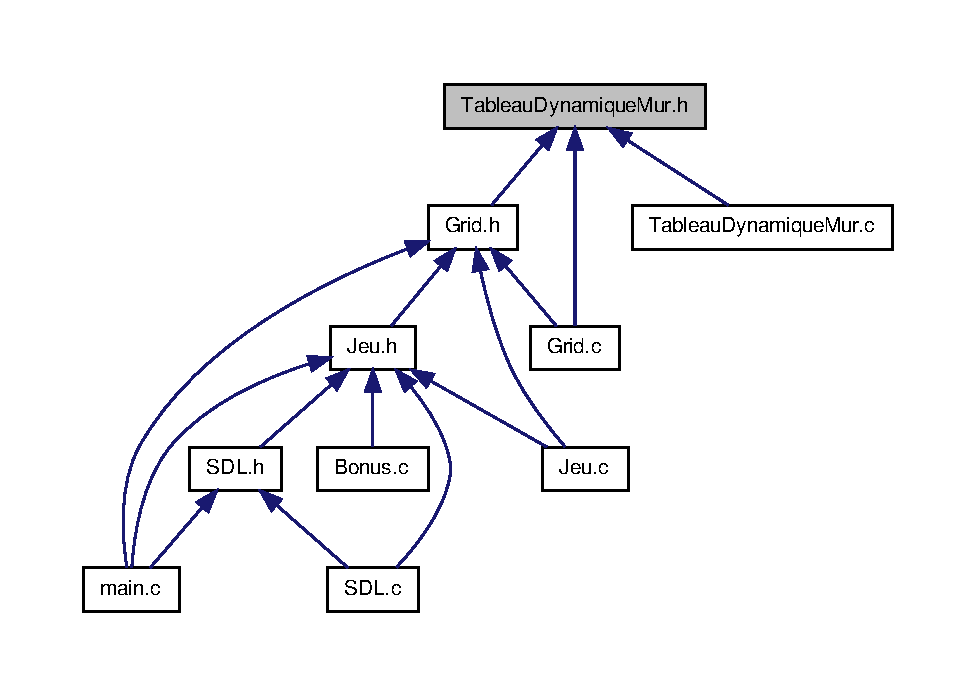
\includegraphics[width=350pt]{_tableau_dynamique_mur_8h__dep__incl}
\end{center}
\end{figure}
\subsection*{Structures de données}
\begin{DoxyCompactItemize}
\item 
struct \hyperlink{struct_tableau_dynamique_mur}{Tableau\-Dynamique\-Mur}
\end{DoxyCompactItemize}
\subsection*{Fonctions}
\begin{DoxyCompactItemize}
\item 
unsigned int \hyperlink{_tableau_dynamique_mur_8h_a9d8993673abb44cb220526fc555b97e6}{Tab\-Dyn\-Mur\-Get\-Capacite} (const \hyperlink{struct_tableau_dynamique_mur}{Tableau\-Dynamique\-Mur} $\ast$Tab\-Dyn\-Mur)
\item 
unsigned int \hyperlink{_tableau_dynamique_mur_8h_aa4cccc53a5d36a7df78f86d878a89d96}{Tab\-Dyn\-Mur\-Get\-Taille\-\_\-utilisee} (const \hyperlink{struct_tableau_dynamique_mur}{Tableau\-Dynamique\-Mur} $\ast$Tab\-Dyn\-Mur)
\item 
\hyperlink{struct_mur}{Mur} $\ast$ \hyperlink{_tableau_dynamique_mur_8h_adcadf52764b8e0f32e4844495e3a6724}{Tab\-Dyn\-Mur\-Get\-Ad} (const \hyperlink{struct_tableau_dynamique_mur}{Tableau\-Dynamique\-Mur} $\ast$Tab\-Dyn\-Mur)
\item 
void \hyperlink{_tableau_dynamique_mur_8h_ac0e544e5c2190470f1c888403dd5e75b}{Tab\-Dyn\-Mur\-Set\-Capacite} (\hyperlink{struct_tableau_dynamique_mur}{Tableau\-Dynamique\-Mur} $\ast$Tab\-Dyn\-Mur, unsigned int capacite)
\item 
void \hyperlink{_tableau_dynamique_mur_8h_a8cab81dcce42531992bc233a0a0c91d1}{Tab\-Dyn\-Mur\-Set\-Taille\-\_\-utilisee} (\hyperlink{struct_tableau_dynamique_mur}{Tableau\-Dynamique\-Mur} $\ast$Tab\-Dyn\-Mur, unsigned int taille)
\item 
void \hyperlink{_tableau_dynamique_mur_8h_a247f1e88f472662f5a794384760ca2bc}{Tab\-Dyn\-Mur\-Set\-Ad} (\hyperlink{struct_tableau_dynamique_mur}{Tableau\-Dynamique\-Mur} $\ast$Tab\-Dyn\-Mur, \hyperlink{struct_mur}{Mur} $\ast$ad)
\item 
void \hyperlink{_tableau_dynamique_mur_8h_a677de455353d6c7d8e49e9d8b765f085}{initialiser\-Tab\-Dyn\-Mur} (\hyperlink{struct_tableau_dynamique_mur}{Tableau\-Dynamique\-Mur} $\ast$t)
\item 
void \hyperlink{_tableau_dynamique_mur_8h_ad33a7af085e713d488c62e232464c025}{testament\-Tab\-Dyn\-Mur} (\hyperlink{struct_tableau_dynamique_mur}{Tableau\-Dynamique\-Mur} $\ast$t)
\item 
void \hyperlink{_tableau_dynamique_mur_8h_a31473231236cf3230f7d6f23dedf2ae9}{affecter\-Tab\-Dyn\-Mur} (\hyperlink{struct_tableau_dynamique_mur}{Tableau\-Dynamique\-Mur} $\ast$t1, const \hyperlink{struct_tableau_dynamique_mur}{Tableau\-Dynamique\-Mur} $\ast$t2)
\item 
unsigned int \hyperlink{_tableau_dynamique_mur_8h_a4385563f59ebc05529139926b3cb642b}{taille\-Utilisee\-Tab\-Dyn\-Mur} (const \hyperlink{struct_tableau_dynamique_mur}{Tableau\-Dynamique\-Mur} $\ast$t)
\item 
\hyperlink{struct_mur}{Mur} \hyperlink{_tableau_dynamique_mur_8h_a4b1cf99f3ab429c58cc4f87134dfb146}{valeur\-Ieme\-Element\-Tab\-Dyn\-Mur} (const \hyperlink{struct_tableau_dynamique_mur}{Tableau\-Dynamique\-Mur} $\ast$t, unsigned int i)
\item 
\hyperlink{struct_mur}{Mur} $\ast$ \hyperlink{_tableau_dynamique_mur_8h_a91faee7eb572734cef6f3b81b9793352}{adresse\-Ieme\-Element\-Tab\-Dyn\-Mur} (const \hyperlink{struct_tableau_dynamique_mur}{Tableau\-Dynamique\-Mur} $\ast$t, unsigned int i)
\item 
void \hyperlink{_tableau_dynamique_mur_8h_a76e95156313a16c5956402a00faac297}{ajouter\-Element\-Tab\-Dyn\-Mur} (\hyperlink{struct_tableau_dynamique_mur}{Tableau\-Dynamique\-Mur} $\ast$t, \hyperlink{struct_mur}{Mur} e)
\item 
void \hyperlink{_tableau_dynamique_mur_8h_ac1f6eb509e569f5887171ec6add66d30}{supprimer\-Element\-Tab\-Dyn\-Mur} (\hyperlink{struct_tableau_dynamique_mur}{Tableau\-Dynamique\-Mur} $\ast$t, int position)
\item 
void \hyperlink{_tableau_dynamique_mur_8h_ac9e49d24407d337a101c5186534ab0d0}{modifier\-Valeur\-Ieme\-Element\-Tab\-Dyn\-Mur} (\hyperlink{struct_tableau_dynamique_mur}{Tableau\-Dynamique\-Mur} $\ast$t, \hyperlink{struct_mur}{Mur} e, unsigned int i)
\item 
void \hyperlink{_tableau_dynamique_mur_8h_a3fcc63bda1a34e187a7a3f3acd420fb2}{inserer\-Element\-Tab\-Dyn\-Mur} (\hyperlink{struct_tableau_dynamique_mur}{Tableau\-Dynamique\-Mur} $\ast$t, \hyperlink{struct_mur}{Mur} e, unsigned int i)
\end{DoxyCompactItemize}


\subsection{Description détaillée}
\mbox{]} Module qui gère les tableaux dynamiques des Murs \begin{DoxyAuthor}{Auteur}
\{Antoine.\-C,Matthieu.\-B\} 
\end{DoxyAuthor}
\begin{DoxyVersion}{Version}
1.\-0 
\end{DoxyVersion}
\begin{DoxyDate}{Date}
19 mars 2013 
\end{DoxyDate}


Définition dans le fichier \hyperlink{_tableau_dynamique_mur_8h_source}{Tableau\-Dynamique\-Mur.\-h}.



\subsection{Documentation des fonctions}
\hypertarget{_tableau_dynamique_mur_8h_a91faee7eb572734cef6f3b81b9793352}{\index{Tableau\-Dynamique\-Mur.\-h@{Tableau\-Dynamique\-Mur.\-h}!adresse\-Ieme\-Element\-Tab\-Dyn\-Mur@{adresse\-Ieme\-Element\-Tab\-Dyn\-Mur}}
\index{adresse\-Ieme\-Element\-Tab\-Dyn\-Mur@{adresse\-Ieme\-Element\-Tab\-Dyn\-Mur}!TableauDynamiqueMur.h@{Tableau\-Dynamique\-Mur.\-h}}
\subsubsection[{adresse\-Ieme\-Element\-Tab\-Dyn\-Mur}]{\setlength{\rightskip}{0pt plus 5cm}{\bf Mur}$\ast$ adresse\-Ieme\-Element\-Tab\-Dyn\-Mur (
\begin{DoxyParamCaption}
\item[{const {\bf Tableau\-Dynamique\-Mur} $\ast$}]{t, }
\item[{unsigned int}]{i}
\end{DoxyParamCaption}
)}}\label{_tableau_dynamique_mur_8h_a91faee7eb572734cef6f3b81b9793352}
Precondition \-: t prealablement initialise, 0 $<$= i $<$ taille\-Utilisee(t) Resultat \-: retourne l'adresse du i+1eme Element\-T\-D de t 

Définition à la ligne 82 du fichier Tableau\-Dynamique\-Mur.\-c.

\hypertarget{_tableau_dynamique_mur_8h_a31473231236cf3230f7d6f23dedf2ae9}{\index{Tableau\-Dynamique\-Mur.\-h@{Tableau\-Dynamique\-Mur.\-h}!affecter\-Tab\-Dyn\-Mur@{affecter\-Tab\-Dyn\-Mur}}
\index{affecter\-Tab\-Dyn\-Mur@{affecter\-Tab\-Dyn\-Mur}!TableauDynamiqueMur.h@{Tableau\-Dynamique\-Mur.\-h}}
\subsubsection[{affecter\-Tab\-Dyn\-Mur}]{\setlength{\rightskip}{0pt plus 5cm}void affecter\-Tab\-Dyn\-Mur (
\begin{DoxyParamCaption}
\item[{{\bf Tableau\-Dynamique\-Mur} $\ast$}]{t1, }
\item[{const {\bf Tableau\-Dynamique\-Mur} $\ast$}]{t2}
\end{DoxyParamCaption}
)}}\label{_tableau_dynamique_mur_8h_a31473231236cf3230f7d6f23dedf2ae9}
Precondition \-: t1 et t2 initialises Postcondition \-: l'ancien contenu de t1 est perdu. t1 et t2 contiennent des sequences d'Element\-T\-D identiques t1 correspond a une copie de t2, les 2 tableaux ont meme capacite, meme taille utilisee, mais sont independants) \hypertarget{_tableau_dynamique_mur_8h_a76e95156313a16c5956402a00faac297}{\index{Tableau\-Dynamique\-Mur.\-h@{Tableau\-Dynamique\-Mur.\-h}!ajouter\-Element\-Tab\-Dyn\-Mur@{ajouter\-Element\-Tab\-Dyn\-Mur}}
\index{ajouter\-Element\-Tab\-Dyn\-Mur@{ajouter\-Element\-Tab\-Dyn\-Mur}!TableauDynamiqueMur.h@{Tableau\-Dynamique\-Mur.\-h}}
\subsubsection[{ajouter\-Element\-Tab\-Dyn\-Mur}]{\setlength{\rightskip}{0pt plus 5cm}void ajouter\-Element\-Tab\-Dyn\-Mur (
\begin{DoxyParamCaption}
\item[{{\bf Tableau\-Dynamique\-Mur} $\ast$}]{t, }
\item[{{\bf Mur}}]{e}
\end{DoxyParamCaption}
)}}\label{_tableau_dynamique_mur_8h_a76e95156313a16c5956402a00faac297}
Precondition \-: t prealablement initialise Postcondition \-: L'element e est ajoute dans la premiere alveole inutilisee du tableau, la taille utilisee est incrementee de 1. Doublement de la capacite de t, si necessaire. 

Définition à la ligne 57 du fichier Tableau\-Dynamique\-Mur.\-c.

\hypertarget{_tableau_dynamique_mur_8h_a677de455353d6c7d8e49e9d8b765f085}{\index{Tableau\-Dynamique\-Mur.\-h@{Tableau\-Dynamique\-Mur.\-h}!initialiser\-Tab\-Dyn\-Mur@{initialiser\-Tab\-Dyn\-Mur}}
\index{initialiser\-Tab\-Dyn\-Mur@{initialiser\-Tab\-Dyn\-Mur}!TableauDynamiqueMur.h@{Tableau\-Dynamique\-Mur.\-h}}
\subsubsection[{initialiser\-Tab\-Dyn\-Mur}]{\setlength{\rightskip}{0pt plus 5cm}void initialiser\-Tab\-Dyn\-Mur (
\begin{DoxyParamCaption}
\item[{{\bf Tableau\-Dynamique\-Mur} $\ast$}]{t}
\end{DoxyParamCaption}
)}}\label{_tableau_dynamique_mur_8h_a677de455353d6c7d8e49e9d8b765f085}
Precondition \-: t non prealablement initialise Postcondition \-: t initialise a une alveole vide (taille utilisee nulle) 

Définition à la ligne 37 du fichier Tableau\-Dynamique\-Mur.\-c.

\hypertarget{_tableau_dynamique_mur_8h_a3fcc63bda1a34e187a7a3f3acd420fb2}{\index{Tableau\-Dynamique\-Mur.\-h@{Tableau\-Dynamique\-Mur.\-h}!inserer\-Element\-Tab\-Dyn\-Mur@{inserer\-Element\-Tab\-Dyn\-Mur}}
\index{inserer\-Element\-Tab\-Dyn\-Mur@{inserer\-Element\-Tab\-Dyn\-Mur}!TableauDynamiqueMur.h@{Tableau\-Dynamique\-Mur.\-h}}
\subsubsection[{inserer\-Element\-Tab\-Dyn\-Mur}]{\setlength{\rightskip}{0pt plus 5cm}void inserer\-Element\-Tab\-Dyn\-Mur (
\begin{DoxyParamCaption}
\item[{{\bf Tableau\-Dynamique\-Mur} $\ast$}]{t, }
\item[{{\bf Mur}}]{e, }
\item[{unsigned int}]{i}
\end{DoxyParamCaption}
)}}\label{_tableau_dynamique_mur_8h_a3fcc63bda1a34e187a7a3f3acd420fb2}
Precondition \-: t prealablement initialise et 0 $<$= i $<$ taille\-Utilisee(t) Postcondition \-: e est insere en i+1eme position et taille\-Utilisee est incrementee de 1 \hypertarget{_tableau_dynamique_mur_8h_ac9e49d24407d337a101c5186534ab0d0}{\index{Tableau\-Dynamique\-Mur.\-h@{Tableau\-Dynamique\-Mur.\-h}!modifier\-Valeur\-Ieme\-Element\-Tab\-Dyn\-Mur@{modifier\-Valeur\-Ieme\-Element\-Tab\-Dyn\-Mur}}
\index{modifier\-Valeur\-Ieme\-Element\-Tab\-Dyn\-Mur@{modifier\-Valeur\-Ieme\-Element\-Tab\-Dyn\-Mur}!TableauDynamiqueMur.h@{Tableau\-Dynamique\-Mur.\-h}}
\subsubsection[{modifier\-Valeur\-Ieme\-Element\-Tab\-Dyn\-Mur}]{\setlength{\rightskip}{0pt plus 5cm}void modifier\-Valeur\-Ieme\-Element\-Tab\-Dyn\-Mur (
\begin{DoxyParamCaption}
\item[{{\bf Tableau\-Dynamique\-Mur} $\ast$}]{t, }
\item[{{\bf Mur}}]{e, }
\item[{unsigned int}]{i}
\end{DoxyParamCaption}
)}}\label{_tableau_dynamique_mur_8h_ac9e49d24407d337a101c5186534ab0d0}
Precondition \-: t prealablement initialise et 0 $<$= i $<$ taille\-Utilisee(t) Postcondition \-: le i+1eme Element\-T\-D de t vaut e 

Définition à la ligne 89 du fichier Tableau\-Dynamique\-Mur.\-c.

\hypertarget{_tableau_dynamique_mur_8h_ac1f6eb509e569f5887171ec6add66d30}{\index{Tableau\-Dynamique\-Mur.\-h@{Tableau\-Dynamique\-Mur.\-h}!supprimer\-Element\-Tab\-Dyn\-Mur@{supprimer\-Element\-Tab\-Dyn\-Mur}}
\index{supprimer\-Element\-Tab\-Dyn\-Mur@{supprimer\-Element\-Tab\-Dyn\-Mur}!TableauDynamiqueMur.h@{Tableau\-Dynamique\-Mur.\-h}}
\subsubsection[{supprimer\-Element\-Tab\-Dyn\-Mur}]{\setlength{\rightskip}{0pt plus 5cm}void supprimer\-Element\-Tab\-Dyn\-Mur (
\begin{DoxyParamCaption}
\item[{{\bf Tableau\-Dynamique\-Mur} $\ast$}]{t, }
\item[{int}]{position}
\end{DoxyParamCaption}
)}}\label{_tableau_dynamique_mur_8h_ac1f6eb509e569f5887171ec6add66d30}
Precondition \-: t prealablement initialise et non vide Postcondition \-: la taille utilisee du tableau est decrementee de 1. Si taille\-Utilisee $<$ capacite/3, alors on divise la capacité par 2. 

Définition à la ligne 99 du fichier Tableau\-Dynamique\-Mur.\-c.

\hypertarget{_tableau_dynamique_mur_8h_adcadf52764b8e0f32e4844495e3a6724}{\index{Tableau\-Dynamique\-Mur.\-h@{Tableau\-Dynamique\-Mur.\-h}!Tab\-Dyn\-Mur\-Get\-Ad@{Tab\-Dyn\-Mur\-Get\-Ad}}
\index{Tab\-Dyn\-Mur\-Get\-Ad@{Tab\-Dyn\-Mur\-Get\-Ad}!TableauDynamiqueMur.h@{Tableau\-Dynamique\-Mur.\-h}}
\subsubsection[{Tab\-Dyn\-Mur\-Get\-Ad}]{\setlength{\rightskip}{0pt plus 5cm}{\bf Mur}$\ast$ Tab\-Dyn\-Mur\-Get\-Ad (
\begin{DoxyParamCaption}
\item[{const {\bf Tableau\-Dynamique\-Mur} $\ast$}]{Tab\-Dyn\-Mur}
\end{DoxyParamCaption}
)}}\label{_tableau_dynamique_mur_8h_adcadf52764b8e0f32e4844495e3a6724}
assesseur de ad 

Définition à la ligne 20 du fichier Tableau\-Dynamique\-Mur.\-c.

\hypertarget{_tableau_dynamique_mur_8h_a9d8993673abb44cb220526fc555b97e6}{\index{Tableau\-Dynamique\-Mur.\-h@{Tableau\-Dynamique\-Mur.\-h}!Tab\-Dyn\-Mur\-Get\-Capacite@{Tab\-Dyn\-Mur\-Get\-Capacite}}
\index{Tab\-Dyn\-Mur\-Get\-Capacite@{Tab\-Dyn\-Mur\-Get\-Capacite}!TableauDynamiqueMur.h@{Tableau\-Dynamique\-Mur.\-h}}
\subsubsection[{Tab\-Dyn\-Mur\-Get\-Capacite}]{\setlength{\rightskip}{0pt plus 5cm}unsigned int Tab\-Dyn\-Mur\-Get\-Capacite (
\begin{DoxyParamCaption}
\item[{const {\bf Tableau\-Dynamique\-Mur} $\ast$}]{Tab\-Dyn\-Mur}
\end{DoxyParamCaption}
)}}\label{_tableau_dynamique_mur_8h_a9d8993673abb44cb220526fc555b97e6}
assesseur de capacite 

Définition à la ligne 14 du fichier Tableau\-Dynamique\-Mur.\-c.

\hypertarget{_tableau_dynamique_mur_8h_aa4cccc53a5d36a7df78f86d878a89d96}{\index{Tableau\-Dynamique\-Mur.\-h@{Tableau\-Dynamique\-Mur.\-h}!Tab\-Dyn\-Mur\-Get\-Taille\-\_\-utilisee@{Tab\-Dyn\-Mur\-Get\-Taille\-\_\-utilisee}}
\index{Tab\-Dyn\-Mur\-Get\-Taille\-\_\-utilisee@{Tab\-Dyn\-Mur\-Get\-Taille\-\_\-utilisee}!TableauDynamiqueMur.h@{Tableau\-Dynamique\-Mur.\-h}}
\subsubsection[{Tab\-Dyn\-Mur\-Get\-Taille\-\_\-utilisee}]{\setlength{\rightskip}{0pt plus 5cm}unsigned int Tab\-Dyn\-Mur\-Get\-Taille\-\_\-utilisee (
\begin{DoxyParamCaption}
\item[{const {\bf Tableau\-Dynamique\-Mur} $\ast$}]{Tab\-Dyn\-Mur}
\end{DoxyParamCaption}
)}}\label{_tableau_dynamique_mur_8h_aa4cccc53a5d36a7df78f86d878a89d96}
assesseur de taille\-\_\-utilisee 

Définition à la ligne 17 du fichier Tableau\-Dynamique\-Mur.\-c.

\hypertarget{_tableau_dynamique_mur_8h_a247f1e88f472662f5a794384760ca2bc}{\index{Tableau\-Dynamique\-Mur.\-h@{Tableau\-Dynamique\-Mur.\-h}!Tab\-Dyn\-Mur\-Set\-Ad@{Tab\-Dyn\-Mur\-Set\-Ad}}
\index{Tab\-Dyn\-Mur\-Set\-Ad@{Tab\-Dyn\-Mur\-Set\-Ad}!TableauDynamiqueMur.h@{Tableau\-Dynamique\-Mur.\-h}}
\subsubsection[{Tab\-Dyn\-Mur\-Set\-Ad}]{\setlength{\rightskip}{0pt plus 5cm}void Tab\-Dyn\-Mur\-Set\-Ad (
\begin{DoxyParamCaption}
\item[{{\bf Tableau\-Dynamique\-Mur} $\ast$}]{Tab\-Dyn\-Mur, }
\item[{{\bf Mur} $\ast$}]{ad}
\end{DoxyParamCaption}
)}}\label{_tableau_dynamique_mur_8h_a247f1e88f472662f5a794384760ca2bc}
mutateur de ad 

Définition à la ligne 30 du fichier Tableau\-Dynamique\-Mur.\-c.

\hypertarget{_tableau_dynamique_mur_8h_ac0e544e5c2190470f1c888403dd5e75b}{\index{Tableau\-Dynamique\-Mur.\-h@{Tableau\-Dynamique\-Mur.\-h}!Tab\-Dyn\-Mur\-Set\-Capacite@{Tab\-Dyn\-Mur\-Set\-Capacite}}
\index{Tab\-Dyn\-Mur\-Set\-Capacite@{Tab\-Dyn\-Mur\-Set\-Capacite}!TableauDynamiqueMur.h@{Tableau\-Dynamique\-Mur.\-h}}
\subsubsection[{Tab\-Dyn\-Mur\-Set\-Capacite}]{\setlength{\rightskip}{0pt plus 5cm}void Tab\-Dyn\-Mur\-Set\-Capacite (
\begin{DoxyParamCaption}
\item[{{\bf Tableau\-Dynamique\-Mur} $\ast$}]{Tab\-Dyn\-Mur, }
\item[{unsigned int}]{capacite}
\end{DoxyParamCaption}
)}}\label{_tableau_dynamique_mur_8h_ac0e544e5c2190470f1c888403dd5e75b}
mutateur de capacite 

Définition à la ligne 24 du fichier Tableau\-Dynamique\-Mur.\-c.

\hypertarget{_tableau_dynamique_mur_8h_a8cab81dcce42531992bc233a0a0c91d1}{\index{Tableau\-Dynamique\-Mur.\-h@{Tableau\-Dynamique\-Mur.\-h}!Tab\-Dyn\-Mur\-Set\-Taille\-\_\-utilisee@{Tab\-Dyn\-Mur\-Set\-Taille\-\_\-utilisee}}
\index{Tab\-Dyn\-Mur\-Set\-Taille\-\_\-utilisee@{Tab\-Dyn\-Mur\-Set\-Taille\-\_\-utilisee}!TableauDynamiqueMur.h@{Tableau\-Dynamique\-Mur.\-h}}
\subsubsection[{Tab\-Dyn\-Mur\-Set\-Taille\-\_\-utilisee}]{\setlength{\rightskip}{0pt plus 5cm}void Tab\-Dyn\-Mur\-Set\-Taille\-\_\-utilisee (
\begin{DoxyParamCaption}
\item[{{\bf Tableau\-Dynamique\-Mur} $\ast$}]{Tab\-Dyn\-Mur, }
\item[{unsigned int}]{taille}
\end{DoxyParamCaption}
)}}\label{_tableau_dynamique_mur_8h_a8cab81dcce42531992bc233a0a0c91d1}
mutateur de taille\-\_\-utilisee 

Définition à la ligne 27 du fichier Tableau\-Dynamique\-Mur.\-c.

\hypertarget{_tableau_dynamique_mur_8h_a4385563f59ebc05529139926b3cb642b}{\index{Tableau\-Dynamique\-Mur.\-h@{Tableau\-Dynamique\-Mur.\-h}!taille\-Utilisee\-Tab\-Dyn\-Mur@{taille\-Utilisee\-Tab\-Dyn\-Mur}}
\index{taille\-Utilisee\-Tab\-Dyn\-Mur@{taille\-Utilisee\-Tab\-Dyn\-Mur}!TableauDynamiqueMur.h@{Tableau\-Dynamique\-Mur.\-h}}
\subsubsection[{taille\-Utilisee\-Tab\-Dyn\-Mur}]{\setlength{\rightskip}{0pt plus 5cm}unsigned int taille\-Utilisee\-Tab\-Dyn\-Mur (
\begin{DoxyParamCaption}
\item[{const {\bf Tableau\-Dynamique\-Mur} $\ast$}]{t}
\end{DoxyParamCaption}
)}}\label{_tableau_dynamique_mur_8h_a4385563f59ebc05529139926b3cb642b}
Precondition \-: t prealablement initialise Resultat \-: nombre d'Element\-T\-Ds stockes dans t \hypertarget{_tableau_dynamique_mur_8h_ad33a7af085e713d488c62e232464c025}{\index{Tableau\-Dynamique\-Mur.\-h@{Tableau\-Dynamique\-Mur.\-h}!testament\-Tab\-Dyn\-Mur@{testament\-Tab\-Dyn\-Mur}}
\index{testament\-Tab\-Dyn\-Mur@{testament\-Tab\-Dyn\-Mur}!TableauDynamiqueMur.h@{Tableau\-Dynamique\-Mur.\-h}}
\subsubsection[{testament\-Tab\-Dyn\-Mur}]{\setlength{\rightskip}{0pt plus 5cm}void testament\-Tab\-Dyn\-Mur (
\begin{DoxyParamCaption}
\item[{{\bf Tableau\-Dynamique\-Mur} $\ast$}]{t}
\end{DoxyParamCaption}
)}}\label{_tableau_dynamique_mur_8h_ad33a7af085e713d488c62e232464c025}
\begin{DoxyVerb}Precondition : t prealablement initialise
\end{DoxyVerb}
 Postcondition \-: t pret a disparaitre. La memoire allouee dynamiquement est liberee. On ne pourra plus appeler les sous-\/programmes qui necessitent que t soit initialise. 

Définition à la ligne 45 du fichier Tableau\-Dynamique\-Mur.\-c.

\hypertarget{_tableau_dynamique_mur_8h_a4b1cf99f3ab429c58cc4f87134dfb146}{\index{Tableau\-Dynamique\-Mur.\-h@{Tableau\-Dynamique\-Mur.\-h}!valeur\-Ieme\-Element\-Tab\-Dyn\-Mur@{valeur\-Ieme\-Element\-Tab\-Dyn\-Mur}}
\index{valeur\-Ieme\-Element\-Tab\-Dyn\-Mur@{valeur\-Ieme\-Element\-Tab\-Dyn\-Mur}!TableauDynamiqueMur.h@{Tableau\-Dynamique\-Mur.\-h}}
\subsubsection[{valeur\-Ieme\-Element\-Tab\-Dyn\-Mur}]{\setlength{\rightskip}{0pt plus 5cm}{\bf Mur} valeur\-Ieme\-Element\-Tab\-Dyn\-Mur (
\begin{DoxyParamCaption}
\item[{const {\bf Tableau\-Dynamique\-Mur} $\ast$}]{t, }
\item[{unsigned int}]{i}
\end{DoxyParamCaption}
)}}\label{_tableau_dynamique_mur_8h_a4b1cf99f3ab429c58cc4f87134dfb146}
Precondition \-: t prealablement initialise, 0 $<$= i $<$ taille\-Utilisee(t) Resultat \-: retourne le i+1eme Element\-T\-D de t 

Définition à la ligne 77 du fichier Tableau\-Dynamique\-Mur.\-c.


\addcontentsline{toc}{part}{Index}
\printindex
\end{document}
